\documentclass{book}
\usepackage[letterpaper,top=2.5cm,bottom=2.5cm,left=2.5cm,right=2.5cm]{geometry}
\usepackage{makeidx}
\usepackage{natbib}
\usepackage{graphicx}
\usepackage{multicol}
\usepackage{float}
\usepackage{listings}
\usepackage{color}
\usepackage{ifthen}
\usepackage[table]{xcolor}
\usepackage{textcomp}
\usepackage{alltt}
\usepackage{ifpdf}
\ifpdf
\usepackage[pdftex,
            pagebackref=true,
            colorlinks=true,
            linkcolor=blue,
            unicode
           ]{hyperref}
\else
\usepackage[ps2pdf,
            pagebackref=true,
            colorlinks=true,
            linkcolor=blue,
            unicode
           ]{hyperref}
\usepackage{pspicture}
\fi
\usepackage[utf8]{inputenc}
\usepackage{mathptmx}
\usepackage[scaled=.90]{helvet}
\usepackage{courier}
\usepackage{sectsty}
\usepackage{amssymb}
\usepackage[titles]{tocloft}
\usepackage{doxygen}
\lstset{language=C++,inputencoding=utf8,basicstyle=\footnotesize,breaklines=true,breakatwhitespace=true,tabsize=4,numbers=left }
\makeindex
\setcounter{tocdepth}{3}
\renewcommand{\footrulewidth}{0.4pt}
\renewcommand{\familydefault}{\sfdefault}
\hfuzz=15pt
\setlength{\emergencystretch}{15pt}
\hbadness=750
\tolerance=750
\begin{document}
\hypersetup{pageanchor=false,citecolor=blue}
\begin{titlepage}
\vspace*{7cm}
\begin{center}
{\Large Sneaky\-F\-S \\[1ex]\large 1.\-0 }\\
\vspace*{1.0cm}
{\large Jonathan Gillett \\ Joseph Heron \\[0.10cm] Daniel Smullen}\\
\vspace*{0.5cm}
{\small Document Revision 1.1}\\
\end{center}
\end{titlepage}
\clearemptydoublepage
\pagenumbering{roman}
\tableofcontents
\clearemptydoublepage
\pagenumbering{arabic}
\hypersetup{pageanchor=true,citecolor=blue}
\chapter{Deprecated List}
\label{deprecated}
\hypertarget{deprecated}{}

\begin{DoxyRefList}
\item[\label{deprecated__deprecated000001}%
\hypertarget{deprecated__deprecated000001}{}%
Global \hyperlink{glob__data_8h_a3178042a14309a5af3336234b7b0a9d1}{U\-N\-I\-T\-\_\-\-T\-E\-S\-T\-I\-N\-G} ]This definition is no longer used since the unit test suite was no longer used and deprecated once the high-\/level file system functions were implemented. 
\end{DoxyRefList}
\chapter{Data Structure Index}
\section{Data Structures}
Here are the data structures with brief descriptions\-:\begin{DoxyCompactList}
\item\contentsline{section}{\hyperlink{structcwd}{cwd} \\*Holds the current working directory data }{\pageref{structcwd}}{}
\item\contentsline{section}{\hyperlink{structdata__index}{data\-\_\-index} }{\pageref{structdata__index}}{}
\item\contentsline{section}{\hyperlink{structfree__block__list}{free\-\_\-block\-\_\-list} \\*The \hyperlink{structfree__block__list}{free\-\_\-block\-\_\-list} is an array containing the free blocks on disk. Elements are marked as free (false), or used (true). The super block always points to the first index block of the \hyperlink{structfree__block__list}{free\-\_\-block\-\_\-list} }{\pageref{structfree__block__list}}{}
\item\contentsline{section}{\hyperlink{structinode}{inode} \\*Contains the data stored in inodes }{\pageref{structinode}}{}
\item\contentsline{section}{\hyperlink{struct_superblock}{Superblock} \\*The superblock contains information pertainent to the disk }{\pageref{struct_superblock}}{}
\item\contentsline{section}{\hyperlink{structsuperblock}{superblock} }{\pageref{structsuperblock}}{}
\item\contentsline{section}{\hyperlink{structswoft}{swoft} \\*Pseudo-\/object containing the array of open file descriptors }{\pageref{structswoft}}{}
\end{DoxyCompactList}

\chapter{File Index}
\section{File List}
Here is a list of all files with brief descriptions\-:\begin{DoxyCompactList}
\item\contentsline{section}{\hyperlink{block__func_8c}{block\-\_\-func.\-c} }{\pageref{block__func_8c}}{}
\item\contentsline{section}{\hyperlink{block__func_8h}{block\-\_\-func.\-h} }{\pageref{block__func_8h}}{}
\item\contentsline{section}{\hyperlink{blockio_8c}{blockio.\-c} }{\pageref{blockio_8c}}{}
\item\contentsline{section}{\hyperlink{blockio_8h}{blockio.\-h} }{\pageref{blockio_8h}}{}
\item\contentsline{section}{\hyperlink{close__file_8c}{close\-\_\-file.\-c} }{\pageref{close__file_8c}}{}
\item\contentsline{section}{\hyperlink{close__file_8h}{close\-\_\-file.\-h} }{\pageref{close__file_8h}}{}
\item\contentsline{section}{\hyperlink{create__file_8c}{create\-\_\-file.\-c} }{\pageref{create__file_8c}}{}
\item\contentsline{section}{\hyperlink{create__file_8h}{create\-\_\-file.\-h} }{\pageref{create__file_8h}}{}
\item\contentsline{section}{\hyperlink{delete__file_8c}{delete\-\_\-file.\-c} }{\pageref{delete__file_8c}}{}
\item\contentsline{section}{\hyperlink{delete__file_8h}{delete\-\_\-file.\-h} }{\pageref{delete__file_8h}}{}
\item\contentsline{section}{\hyperlink{error_8c}{error.\-c} }{\pageref{error_8c}}{}
\item\contentsline{section}{\hyperlink{error_8h}{error.\-h} }{\pageref{error_8h}}{}
\item\contentsline{section}{\hyperlink{free__block__list_8c}{free\-\_\-block\-\_\-list.\-c} }{\pageref{free__block__list_8c}}{}
\item\contentsline{section}{\hyperlink{free__block__list_8h}{free\-\_\-block\-\_\-list.\-h} }{\pageref{free__block__list_8h}}{}
\item\contentsline{section}{\hyperlink{get__size_8c}{get\-\_\-size.\-c} }{\pageref{get__size_8c}}{}
\item\contentsline{section}{\hyperlink{get__size_8h}{get\-\_\-size.\-h} }{\pageref{get__size_8h}}{}
\item\contentsline{section}{\hyperlink{get__type_8c}{get\-\_\-type.\-c} }{\pageref{get__type_8c}}{}
\item\contentsline{section}{\hyperlink{get__type_8h}{get\-\_\-type.\-h} }{\pageref{get__type_8h}}{}
\item\contentsline{section}{\hyperlink{glob__data_8h}{glob\-\_\-data.\-h} }{\pageref{glob__data_8h}}{}
\item\contentsline{section}{\hyperlink{glob__func_8c}{glob\-\_\-func.\-c} }{\pageref{glob__func_8c}}{}
\item\contentsline{section}{\hyperlink{glob__func_8h}{glob\-\_\-func.\-h} }{\pageref{glob__func_8h}}{}
\item\contentsline{section}{\hyperlink{_i__node_8c}{I\-\_\-node.\-c} }{\pageref{_i__node_8c}}{}
\item\contentsline{section}{\hyperlink{_i__node_8h}{I\-\_\-node.\-h} }{\pageref{_i__node_8h}}{}
\item\contentsline{section}{\hyperlink{index__block_8c}{index\-\_\-block.\-c} }{\pageref{index__block_8c}}{}
\item\contentsline{section}{\hyperlink{index__block_8h}{index\-\_\-block.\-h} }{\pageref{index__block_8h}}{}
\item\contentsline{section}{\hyperlink{initialize_8c}{initialize.\-c} }{\pageref{initialize_8c}}{}
\item\contentsline{section}{\hyperlink{initialize_8h}{initialize.\-h} }{\pageref{initialize_8h}}{}
\item\contentsline{section}{\hyperlink{mount_8c}{mount.\-c} }{\pageref{mount_8c}}{}
\item\contentsline{section}{\hyperlink{mount_8h}{mount.\-h} }{\pageref{mount_8h}}{}
\item\contentsline{section}{\hyperlink{open__file_8c}{open\-\_\-file.\-c} }{\pageref{open__file_8c}}{}
\item\contentsline{section}{\hyperlink{open__file_8h}{open\-\_\-file.\-h} }{\pageref{open__file_8h}}{}
\item\contentsline{section}{\hyperlink{read__dir_8c}{read\-\_\-dir.\-c} }{\pageref{read__dir_8c}}{}
\item\contentsline{section}{\hyperlink{read__dir_8h}{read\-\_\-dir.\-h} }{\pageref{read__dir_8h}}{}
\item\contentsline{section}{\hyperlink{read__file_8c}{read\-\_\-file.\-c} }{\pageref{read__file_8c}}{}
\item\contentsline{section}{\hyperlink{read__file_8h}{read\-\_\-file.\-h} }{\pageref{read__file_8h}}{}
\item\contentsline{section}{\hyperlink{sfstest_8c}{sfstest.\-c} }{\pageref{sfstest_8c}}{}
\item\contentsline{section}{\hyperlink{super__block_8c}{super\-\_\-block.\-c} }{\pageref{super__block_8c}}{}
\item\contentsline{section}{\hyperlink{super__block_8h}{super\-\_\-block.\-h} }{\pageref{super__block_8h}}{}
\item\contentsline{section}{\hyperlink{system__open__file__table_8c}{system\-\_\-open\-\_\-file\-\_\-table.\-c} }{\pageref{system__open__file__table_8c}}{}
\item\contentsline{section}{\hyperlink{system__open__file__table_8h}{system\-\_\-open\-\_\-file\-\_\-table.\-h} }{\pageref{system__open__file__table_8h}}{}
\item\contentsline{section}{\hyperlink{traverse__tree_8c}{traverse\-\_\-tree.\-c} }{\pageref{traverse__tree_8c}}{}
\item\contentsline{section}{\hyperlink{traverse__tree_8h}{traverse\-\_\-tree.\-h} }{\pageref{traverse__tree_8h}}{}
\item\contentsline{section}{\hyperlink{write__file_8c}{write\-\_\-file.\-c} }{\pageref{write__file_8c}}{}
\item\contentsline{section}{\hyperlink{write__file_8h}{write\-\_\-file.\-h} }{\pageref{write__file_8h}}{}
\end{DoxyCompactList}

\chapter{Data Structure Documentation}
\hypertarget{structcwd}{\section{cwd Struct Reference}
\label{structcwd}\index{cwd@{cwd}}
}


Holds the current working directory data.  




{\ttfamily \#include $<$I\-\_\-node.\-h$>$}



Collaboration diagram for cwd\-:
\nopagebreak
\begin{figure}[H]
\begin{center}
\leavevmode
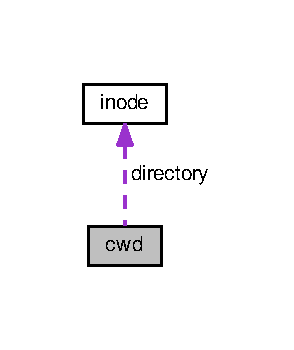
\includegraphics[width=141pt]{structcwd__coll__graph}
\end{center}
\end{figure}
\subsection*{Data Fields}
\begin{DoxyCompactItemize}
\item 
\hyperlink{structinode}{inode} \hyperlink{structcwd_a09a79f07c0f19843fbe3e5277106c8db}{directory}
\item 
uint32\-\_\-t \hyperlink{structcwd_af9f19a44a251a4b45c3e949b698b9294}{cur\-\_\-index}
\end{DoxyCompactItemize}


\subsection{Detailed Description}
Holds the current working directory data. 

This struct holds the current working directory in memory. It is used in a pseudo-\/object oriented fashion in order to encapsulate the data pertaining to the contents of the current working directory and the last directory element that was retrieved from reading the directory contents.

\begin{DoxyAuthor}{Author}
Daniel Smullen

Jonathan Gillett

Joseph Heron
\end{DoxyAuthor}
\begin{DoxyCopyright}{Copyright}
G\-N\-U General Public License V3 
\end{DoxyCopyright}


\subsection{Field Documentation}
\hypertarget{structcwd_af9f19a44a251a4b45c3e949b698b9294}{\index{cwd@{cwd}!cur\-\_\-index@{cur\-\_\-index}}
\index{cur\-\_\-index@{cur\-\_\-index}!cwd@{cwd}}
\subsubsection[{cur\-\_\-index}]{\setlength{\rightskip}{0pt plus 5cm}uint32\-\_\-t cur\-\_\-index}}\label{structcwd_af9f19a44a251a4b45c3e949b698b9294}
This contains the inode for the current working directory. \hypertarget{structcwd_a09a79f07c0f19843fbe3e5277106c8db}{\index{cwd@{cwd}!directory@{directory}}
\index{directory@{directory}!cwd@{cwd}}
\subsubsection[{directory}]{\setlength{\rightskip}{0pt plus 5cm}{\bf inode} directory}}\label{structcwd_a09a79f07c0f19843fbe3e5277106c8db}


The documentation for this struct was generated from the following file\-:\begin{DoxyCompactItemize}
\item 
\hyperlink{_i__node_8h}{I\-\_\-node.\-h}\end{DoxyCompactItemize}

\hypertarget{structdata__index}{\section{data\-\_\-index Struct Reference}
\label{structdata__index}\index{data\-\_\-index@{data\-\_\-index}}
}


{\ttfamily \#include $<$index\-\_\-block.\-h$>$}

\subsection*{Data Fields}
\begin{DoxyCompactItemize}
\item 
uint32\-\_\-t \hyperlink{structdata__index_a9f7ac2c27413909a97f1ba11bfd7ff98}{index\-\_\-location}
\item 
\hyperlink{glob__data_8h_a9d4937e46b9fac69334d5fc7ea3f37a6}{locations} \hyperlink{structdata__index_ae3cb32a3d2f9b47cbd3909eb7aec6a9b}{data\-\_\-locations}
\end{DoxyCompactItemize}


\subsection{Field Documentation}
\hypertarget{structdata__index_ae3cb32a3d2f9b47cbd3909eb7aec6a9b}{\index{data\-\_\-index@{data\-\_\-index}!data\-\_\-locations@{data\-\_\-locations}}
\index{data\-\_\-locations@{data\-\_\-locations}!data_index@{data\-\_\-index}}
\subsubsection[{data\-\_\-locations}]{\setlength{\rightskip}{0pt plus 5cm}{\bf locations} data\-\_\-locations}}\label{structdata__index_ae3cb32a3d2f9b47cbd3909eb7aec6a9b}
\hypertarget{structdata__index_a9f7ac2c27413909a97f1ba11bfd7ff98}{\index{data\-\_\-index@{data\-\_\-index}!index\-\_\-location@{index\-\_\-location}}
\index{index\-\_\-location@{index\-\_\-location}!data_index@{data\-\_\-index}}
\subsubsection[{index\-\_\-location}]{\setlength{\rightskip}{0pt plus 5cm}uint32\-\_\-t index\-\_\-location}}\label{structdata__index_a9f7ac2c27413909a97f1ba11bfd7ff98}


The documentation for this struct was generated from the following file\-:\begin{DoxyCompactItemize}
\item 
\hyperlink{index__block_8h}{index\-\_\-block.\-h}\end{DoxyCompactItemize}

\hypertarget{structfree__block__list}{\section{free\-\_\-block\-\_\-list Struct Reference}
\label{structfree__block__list}\index{free\-\_\-block\-\_\-list@{free\-\_\-block\-\_\-list}}
}


The \hyperlink{structfree__block__list}{free\-\_\-block\-\_\-list} is an array containing the free blocks on disk. Elements are marked as free (false), or used (true). The super block always points to the first index block of the \hyperlink{structfree__block__list}{free\-\_\-block\-\_\-list}.  




{\ttfamily \#include $<$free\-\_\-block\-\_\-list.\-h$>$}

\subsection*{Data Fields}
\begin{DoxyCompactItemize}
\item 
bool \hyperlink{structfree__block__list_afc18ca7178c4649e347e2bc5d69eb89c}{free\-\_\-blocks} \mbox{[}\hyperlink{glob__data_8h_a1a26eed02f4dee88f68eb825c8ace393}{N\-U\-M\-B\-L\-K\-S}\mbox{]}
\end{DoxyCompactItemize}


\subsection{Detailed Description}
The \hyperlink{structfree__block__list}{free\-\_\-block\-\_\-list} is an array containing the free blocks on disk. Elements are marked as free (false), or used (true). The super block always points to the first index block of the \hyperlink{structfree__block__list}{free\-\_\-block\-\_\-list}. 

\subsection{Field Documentation}
\hypertarget{structfree__block__list_afc18ca7178c4649e347e2bc5d69eb89c}{\index{free\-\_\-block\-\_\-list@{free\-\_\-block\-\_\-list}!free\-\_\-blocks@{free\-\_\-blocks}}
\index{free\-\_\-blocks@{free\-\_\-blocks}!free_block_list@{free\-\_\-block\-\_\-list}}
\subsubsection[{free\-\_\-blocks}]{\setlength{\rightskip}{0pt plus 5cm}bool free\-\_\-blocks\mbox{[}{\bf N\-U\-M\-B\-L\-K\-S}\mbox{]}}}\label{structfree__block__list_afc18ca7178c4649e347e2bc5d69eb89c}


The documentation for this struct was generated from the following file\-:\begin{DoxyCompactItemize}
\item 
\hyperlink{free__block__list_8h}{free\-\_\-block\-\_\-list.\-h}\end{DoxyCompactItemize}

\hypertarget{structinode}{\section{inode Struct Reference}
\label{structinode}\index{inode@{inode}}
}


Contains the data stored in inodes.  




{\ttfamily \#include $<$I\-\_\-node.\-h$>$}

\subsection*{Data Fields}
\begin{DoxyCompactItemize}
\item 
char \hyperlink{structinode_af869a309a32425813b56b839f9659b24}{name} \mbox{[}\hyperlink{glob__data_8h_afd709f201d7643c3909621f620ea648a}{M\-A\-X\-\_\-\-N\-A\-M\-E\-\_\-\-L\-E\-N}\mbox{]}
\item 
bool \hyperlink{structinode_a565421f589059ae13581e05b505cf5f0}{type}
\item 
bool \hyperlink{structinode_af49a80be54293d8b153cd2a3dfd4e068}{read}
\item 
bool \hyperlink{structinode_ab4d8d1259f524270d625ab8933700d27}{write}
\item 
bool \hyperlink{structinode_a253e08d8b620206d485babf8a40d53db}{execute}
\item 
time\-\_\-t \hyperlink{structinode_a6fcc067af656e07c0d52cb7890be4a1f}{date\-\_\-of\-\_\-create}
\item 
time\-\_\-t \hyperlink{structinode_a3b1b10b96addbc06de562360c44d44c2}{date\-\_\-last\-\_\-accessed}
\item 
time\-\_\-t \hyperlink{structinode_a6c79d9f7a8c07080347292608eff8cbd}{date\-\_\-last\-\_\-modified}
\item 
uint32\-\_\-t \hyperlink{structinode_a3f405dba01154bed631df46b0a27d593}{file\-\_\-owner}
\item 
uint32\-\_\-t \hyperlink{structinode_a735957d2fe21c7a191634c86079317d0}{last\-\_\-user\-\_\-modified}
\item 
uint32\-\_\-t \hyperlink{structinode_acfc905fb689f590842c0152e3b8cd92e}{file\-\_\-size}
\item 
uint32\-\_\-t \hyperlink{structinode_a8f37ff59738c23420be43a6b1ba69769}{location}
\item 
bool \hyperlink{structinode_a8a32018f1892e247f08ea9a91f5505e6}{encrypted}
\item 
uint32\-\_\-t \hyperlink{structinode_a609a9abb9ba167b63027aad986198118}{check\-\_\-sum}
\item 
uuid\-\_\-t \hyperlink{structinode_a0c9cfc131b27ae3b98b1533bba4c58ef}{uuid}
\end{DoxyCompactItemize}


\subsection{Detailed Description}
Contains the data stored in inodes. 

This struct defines the data which will be stored inside blocks designated as inodes on the disk. In particular, inodes store data pertaining to the attributes of they files they represent, as well as linkages to the index block structure that allows the file system to track their associated data blocks. Since files can be either a directory or a data file, inodes provide all the data required to track both types of data structures.

\begin{DoxyAuthor}{Author}
Daniel Smullen

Jonathan Gillett

Joseph Heron
\end{DoxyAuthor}
\begin{DoxyCopyright}{Copyright}
G\-N\-U General Public License V3 
\end{DoxyCopyright}


\subsection{Field Documentation}
\hypertarget{structinode_a609a9abb9ba167b63027aad986198118}{\index{inode@{inode}!check\-\_\-sum@{check\-\_\-sum}}
\index{check\-\_\-sum@{check\-\_\-sum}!inode@{inode}}
\subsubsection[{check\-\_\-sum}]{\setlength{\rightskip}{0pt plus 5cm}uint32\-\_\-t check\-\_\-sum}}\label{structinode_a609a9abb9ba167b63027aad986198118}
This flags whether the file's data contents are encrypted. \hypertarget{structinode_a3b1b10b96addbc06de562360c44d44c2}{\index{inode@{inode}!date\-\_\-last\-\_\-accessed@{date\-\_\-last\-\_\-accessed}}
\index{date\-\_\-last\-\_\-accessed@{date\-\_\-last\-\_\-accessed}!inode@{inode}}
\subsubsection[{date\-\_\-last\-\_\-accessed}]{\setlength{\rightskip}{0pt plus 5cm}time\-\_\-t date\-\_\-last\-\_\-accessed}}\label{structinode_a3b1b10b96addbc06de562360c44d44c2}
This stores what the date of creation is for the file in P\-O\-S\-I\-X time format. \hypertarget{structinode_a6c79d9f7a8c07080347292608eff8cbd}{\index{inode@{inode}!date\-\_\-last\-\_\-modified@{date\-\_\-last\-\_\-modified}}
\index{date\-\_\-last\-\_\-modified@{date\-\_\-last\-\_\-modified}!inode@{inode}}
\subsubsection[{date\-\_\-last\-\_\-modified}]{\setlength{\rightskip}{0pt plus 5cm}time\-\_\-t date\-\_\-last\-\_\-modified}}\label{structinode_a6c79d9f7a8c07080347292608eff8cbd}
This stores the date that the file was last accessed by the file system in P\-O\-S\-I\-X time format. \hypertarget{structinode_a6fcc067af656e07c0d52cb7890be4a1f}{\index{inode@{inode}!date\-\_\-of\-\_\-create@{date\-\_\-of\-\_\-create}}
\index{date\-\_\-of\-\_\-create@{date\-\_\-of\-\_\-create}!inode@{inode}}
\subsubsection[{date\-\_\-of\-\_\-create}]{\setlength{\rightskip}{0pt plus 5cm}time\-\_\-t date\-\_\-of\-\_\-create}}\label{structinode_a6fcc067af656e07c0d52cb7890be4a1f}
This flags whether the file is marked as executable or not. \hypertarget{structinode_a8a32018f1892e247f08ea9a91f5505e6}{\index{inode@{inode}!encrypted@{encrypted}}
\index{encrypted@{encrypted}!inode@{inode}}
\subsubsection[{encrypted}]{\setlength{\rightskip}{0pt plus 5cm}bool encrypted}}\label{structinode_a8a32018f1892e247f08ea9a91f5505e6}
This stores the location of the file's first index block on disk. \hypertarget{structinode_a253e08d8b620206d485babf8a40d53db}{\index{inode@{inode}!execute@{execute}}
\index{execute@{execute}!inode@{inode}}
\subsubsection[{execute}]{\setlength{\rightskip}{0pt plus 5cm}bool execute}}\label{structinode_a253e08d8b620206d485babf8a40d53db}
This flags whether the file is marked as writable or not. \hypertarget{structinode_a3f405dba01154bed631df46b0a27d593}{\index{inode@{inode}!file\-\_\-owner@{file\-\_\-owner}}
\index{file\-\_\-owner@{file\-\_\-owner}!inode@{inode}}
\subsubsection[{file\-\_\-owner}]{\setlength{\rightskip}{0pt plus 5cm}uint32\-\_\-t file\-\_\-owner}}\label{structinode_a3f405dba01154bed631df46b0a27d593}
This stores the date that the file was last modified by the file system in P\-O\-S\-I\-X time format. \hypertarget{structinode_acfc905fb689f590842c0152e3b8cd92e}{\index{inode@{inode}!file\-\_\-size@{file\-\_\-size}}
\index{file\-\_\-size@{file\-\_\-size}!inode@{inode}}
\subsubsection[{file\-\_\-size}]{\setlength{\rightskip}{0pt plus 5cm}uint32\-\_\-t file\-\_\-size}}\label{structinode_acfc905fb689f590842c0152e3b8cd92e}
This stores the name of the last user who modified the file. \hypertarget{structinode_a735957d2fe21c7a191634c86079317d0}{\index{inode@{inode}!last\-\_\-user\-\_\-modified@{last\-\_\-user\-\_\-modified}}
\index{last\-\_\-user\-\_\-modified@{last\-\_\-user\-\_\-modified}!inode@{inode}}
\subsubsection[{last\-\_\-user\-\_\-modified}]{\setlength{\rightskip}{0pt plus 5cm}uint32\-\_\-t last\-\_\-user\-\_\-modified}}\label{structinode_a735957d2fe21c7a191634c86079317d0}
This stores the name of the owner of the file. \hypertarget{structinode_a8f37ff59738c23420be43a6b1ba69769}{\index{inode@{inode}!location@{location}}
\index{location@{location}!inode@{inode}}
\subsubsection[{location}]{\setlength{\rightskip}{0pt plus 5cm}uint32\-\_\-t location}}\label{structinode_a8f37ff59738c23420be43a6b1ba69769}
This stores the size of the file in bytes. \hypertarget{structinode_af869a309a32425813b56b839f9659b24}{\index{inode@{inode}!name@{name}}
\index{name@{name}!inode@{inode}}
\subsubsection[{name}]{\setlength{\rightskip}{0pt plus 5cm}char name\mbox{[}{\bf M\-A\-X\-\_\-\-N\-A\-M\-E\-\_\-\-L\-E\-N}\mbox{]}}}\label{structinode_af869a309a32425813b56b839f9659b24}
\hypertarget{structinode_af49a80be54293d8b153cd2a3dfd4e068}{\index{inode@{inode}!read@{read}}
\index{read@{read}!inode@{inode}}
\subsubsection[{read}]{\setlength{\rightskip}{0pt plus 5cm}bool read}}\label{structinode_af49a80be54293d8b153cd2a3dfd4e068}
The type of file. Files can be either data files, or directories. \hypertarget{structinode_a565421f589059ae13581e05b505cf5f0}{\index{inode@{inode}!type@{type}}
\index{type@{type}!inode@{inode}}
\subsubsection[{type}]{\setlength{\rightskip}{0pt plus 5cm}bool type}}\label{structinode_a565421f589059ae13581e05b505cf5f0}
The human-\/readable name of the file. \hypertarget{structinode_a0c9cfc131b27ae3b98b1533bba4c58ef}{\index{inode@{inode}!uuid@{uuid}}
\index{uuid@{uuid}!inode@{inode}}
\subsubsection[{uuid}]{\setlength{\rightskip}{0pt plus 5cm}uuid\-\_\-t uuid}}\label{structinode_a0c9cfc131b27ae3b98b1533bba4c58ef}
This stores the encryption checksum for the file, to determine whether it has been encrypted or unencrypted correctly. \hypertarget{structinode_ab4d8d1259f524270d625ab8933700d27}{\index{inode@{inode}!write@{write}}
\index{write@{write}!inode@{inode}}
\subsubsection[{write}]{\setlength{\rightskip}{0pt plus 5cm}bool write}}\label{structinode_ab4d8d1259f524270d625ab8933700d27}
This flags whether the file is marked as readable or not. 

The documentation for this struct was generated from the following file\-:\begin{DoxyCompactItemize}
\item 
\hyperlink{_i__node_8h}{I\-\_\-node.\-h}\end{DoxyCompactItemize}

\hypertarget{struct_superblock}{\section{Superblock Struct Reference}
\label{struct_superblock}\index{Superblock@{Superblock}}
}


The superblock contains information pertainent to the disk.  




{\ttfamily \#include $<$super\-\_\-block.\-h$>$}



\subsection{Detailed Description}
The superblock contains information pertainent to the disk. 

This struct defines the data which will be stored inside the super block. In particular, the super block contains information pertaining to disk attributes, and links to critical file system data structures.

\begin{DoxyAuthor}{Author}
Daniel Smullen

Jonathan Gillett

Joseph Heron
\end{DoxyAuthor}
\begin{DoxyCopyright}{Copyright}
G\-N\-U General Public License V3 
\end{DoxyCopyright}


The documentation for this struct was generated from the following file\-:\begin{DoxyCompactItemize}
\item 
\hyperlink{super__block_8h}{super\-\_\-block.\-h}\end{DoxyCompactItemize}

\hypertarget{structsuperblock}{\section{superblock Struct Reference}
\label{structsuperblock}\index{superblock@{superblock}}
}


{\ttfamily \#include $<$super\-\_\-block.\-h$>$}

\subsection*{Data Fields}
\begin{DoxyCompactItemize}
\item 
uint32\-\_\-t \hyperlink{structsuperblock_a42dadb3b15d8f871bf1bc132b1ede650}{size\-\_\-of\-\_\-disk}
\item 
uint32\-\_\-t \hyperlink{structsuperblock_a9e3fb1e50a1c71b2337df296222d9553}{block\-\_\-size}
\item 
uint32\-\_\-t \hyperlink{structsuperblock_a1ca5e6fd54241f9c2f848530a51bf66c}{free\-\_\-block\-\_\-list}
\item 
uint32\-\_\-t \hyperlink{structsuperblock_aec71d39272df61eb33d94a4675d349be}{root\-\_\-dir}
\item 
uint32\-\_\-t \hyperlink{structsuperblock_a658c495cd1900eadce3b800e3ebdac7a}{device\-\_\-id}
\item 
uuid\-\_\-t \hyperlink{structsuperblock_a0c9cfc131b27ae3b98b1533bba4c58ef}{uuid}
\end{DoxyCompactItemize}


\subsection{Field Documentation}
\hypertarget{structsuperblock_a9e3fb1e50a1c71b2337df296222d9553}{\index{superblock@{superblock}!block\-\_\-size@{block\-\_\-size}}
\index{block\-\_\-size@{block\-\_\-size}!superblock@{superblock}}
\subsubsection[{block\-\_\-size}]{\setlength{\rightskip}{0pt plus 5cm}uint32\-\_\-t block\-\_\-size}}\label{structsuperblock_a9e3fb1e50a1c71b2337df296222d9553}
Total number of blocks on the disk. \hypertarget{structsuperblock_a658c495cd1900eadce3b800e3ebdac7a}{\index{superblock@{superblock}!device\-\_\-id@{device\-\_\-id}}
\index{device\-\_\-id@{device\-\_\-id}!superblock@{superblock}}
\subsubsection[{device\-\_\-id}]{\setlength{\rightskip}{0pt plus 5cm}uint32\-\_\-t device\-\_\-id}}\label{structsuperblock_a658c495cd1900eadce3b800e3ebdac7a}
Location of the root directory's inode on disk. \hypertarget{structsuperblock_a1ca5e6fd54241f9c2f848530a51bf66c}{\index{superblock@{superblock}!free\-\_\-block\-\_\-list@{free\-\_\-block\-\_\-list}}
\index{free\-\_\-block\-\_\-list@{free\-\_\-block\-\_\-list}!superblock@{superblock}}
\subsubsection[{free\-\_\-block\-\_\-list}]{\setlength{\rightskip}{0pt plus 5cm}uint32\-\_\-t {\bf free\-\_\-block\-\_\-list}}}\label{structsuperblock_a1ca5e6fd54241f9c2f848530a51bf66c}
Block size of the disk, in bytes per block. \hypertarget{structsuperblock_aec71d39272df61eb33d94a4675d349be}{\index{superblock@{superblock}!root\-\_\-dir@{root\-\_\-dir}}
\index{root\-\_\-dir@{root\-\_\-dir}!superblock@{superblock}}
\subsubsection[{root\-\_\-dir}]{\setlength{\rightskip}{0pt plus 5cm}uint32\-\_\-t root\-\_\-dir}}\label{structsuperblock_aec71d39272df61eb33d94a4675d349be}
Location of the free block list data structure on disk. \hypertarget{structsuperblock_a42dadb3b15d8f871bf1bc132b1ede650}{\index{superblock@{superblock}!size\-\_\-of\-\_\-disk@{size\-\_\-of\-\_\-disk}}
\index{size\-\_\-of\-\_\-disk@{size\-\_\-of\-\_\-disk}!superblock@{superblock}}
\subsubsection[{size\-\_\-of\-\_\-disk}]{\setlength{\rightskip}{0pt plus 5cm}uint32\-\_\-t size\-\_\-of\-\_\-disk}}\label{structsuperblock_a42dadb3b15d8f871bf1bc132b1ede650}
\hypertarget{structsuperblock_a0c9cfc131b27ae3b98b1533bba4c58ef}{\index{superblock@{superblock}!uuid@{uuid}}
\index{uuid@{uuid}!superblock@{superblock}}
\subsubsection[{uuid}]{\setlength{\rightskip}{0pt plus 5cm}uuid\-\_\-t uuid}}\label{structsuperblock_a0c9cfc131b27ae3b98b1533bba4c58ef}
Device identifier for the disk. No longer required since U\-U\-I\-D was implemented. 

The documentation for this struct was generated from the following file\-:\begin{DoxyCompactItemize}
\item 
\hyperlink{super__block_8h}{super\-\_\-block.\-h}\end{DoxyCompactItemize}

\hypertarget{structswoft}{\section{swoft Struct Reference}
\label{structswoft}\index{swoft@{swoft}}
}


Pseudo-\/object containing the array of open file descriptors.  




{\ttfamily \#include $<$system\-\_\-open\-\_\-file\-\_\-table.\-h$>$}

\subsection*{Data Fields}
\begin{DoxyCompactItemize}
\item 
uint32\-\_\-t \hyperlink{structswoft_a9d67be2cf79bebabe7084963238d6340}{fd} \mbox{[}\hyperlink{glob__data_8h_a8cb920b3b277c4d76122688e1177883d}{N\-U\-M\-O\-F\-L}\mbox{]}
\item 
bool \hyperlink{structswoft_a7d989b9d4ff7182b0fe7b396fd704a46}{taken} \mbox{[}\hyperlink{glob__data_8h_a8cb920b3b277c4d76122688e1177883d}{N\-U\-M\-O\-F\-L}\mbox{]}
\end{DoxyCompactItemize}


\subsection{Detailed Description}
Pseudo-\/object containing the array of open file descriptors. 

The system wide open file table contains an array of file descriptors, which are locations of inodes that have been read from the disk into memory. These are used as handles to the files which exist on disk, and are synchronized with the data on disk upon modification. One instance needs to exist per file.

\begin{DoxyAuthor}{Author}
Daniel Smullen

Jonathan Gillett

Joseph Heron
\end{DoxyAuthor}
\begin{DoxyCopyright}{Copyright}
G\-N\-U General Public License V3 
\end{DoxyCopyright}


\subsection{Field Documentation}
\hypertarget{structswoft_a9d67be2cf79bebabe7084963238d6340}{\index{swoft@{swoft}!fd@{fd}}
\index{fd@{fd}!swoft@{swoft}}
\subsubsection[{fd}]{\setlength{\rightskip}{0pt plus 5cm}uint32\-\_\-t fd\mbox{[}{\bf N\-U\-M\-O\-F\-L}\mbox{]}}}\label{structswoft_a9d67be2cf79bebabe7084963238d6340}
\hypertarget{structswoft_a7d989b9d4ff7182b0fe7b396fd704a46}{\index{swoft@{swoft}!taken@{taken}}
\index{taken@{taken}!swoft@{swoft}}
\subsubsection[{taken}]{\setlength{\rightskip}{0pt plus 5cm}bool taken\mbox{[}{\bf N\-U\-M\-O\-F\-L}\mbox{]}}}\label{structswoft_a7d989b9d4ff7182b0fe7b396fd704a46}


The documentation for this struct was generated from the following file\-:\begin{DoxyCompactItemize}
\item 
\hyperlink{system__open__file__table_8h}{system\-\_\-open\-\_\-file\-\_\-table.\-h}\end{DoxyCompactItemize}

\chapter{File Documentation}
\hypertarget{block__func_8c}{\section{block\-\_\-func.\-c File Reference}
\label{block__func_8c}\index{block\-\_\-func.\-c@{block\-\_\-func.\-c}}
}
{\ttfamily \#include \char`\"{}block\-\_\-func.\-h\char`\"{}}\\*
Include dependency graph for block\-\_\-func.\-c\-:
\nopagebreak
\begin{figure}[H]
\begin{center}
\leavevmode
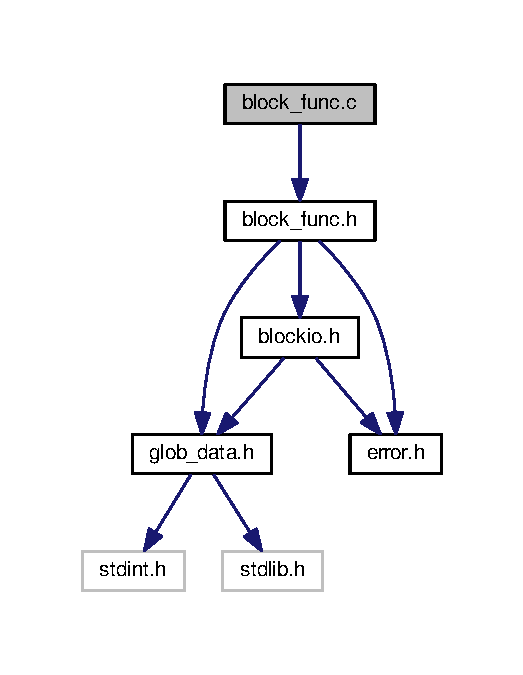
\includegraphics[width=251pt]{block__func_8c__incl}
\end{center}
\end{figure}
\subsection*{Functions}
\begin{DoxyCompactItemize}
\item 
int \hyperlink{block__func_8c_a8d2c516f00e918d009b5fbaf1cfa463b}{write\-\_\-block} (uint32\-\_\-t location, \hyperlink{glob__data_8h_a82b52bf2b45e214a8f2100ebfdf1aee4}{byte} $\ast$buf)
\begin{DoxyCompactList}\small\item\em A wrapper for the put\-\_\-block function. \end{DoxyCompactList}\item 
int \hyperlink{block__func_8c_a1dcadd38a012a1218ab2100bda116861}{read\-\_\-block} (uint32\-\_\-t location, \hyperlink{glob__data_8h_a82b52bf2b45e214a8f2100ebfdf1aee4}{byte} $\ast$buf)
\begin{DoxyCompactList}\small\item\em A wrapper for the get\-\_\-block function. \end{DoxyCompactList}\item 
\hyperlink{glob__data_8h_a82b52bf2b45e214a8f2100ebfdf1aee4}{byte} $\ast$ \hyperlink{block__func_8c_a758063a96fe0be00a4b59b9869a0af62}{get\-\_\-data} (\hyperlink{glob__data_8h_a9d4937e46b9fac69334d5fc7ea3f37a6}{locations} location)
\begin{DoxyCompactList}\small\item\em Get the data blocks and concatenate them into a large byte buffer. \end{DoxyCompactList}\end{DoxyCompactItemize}


\subsection{Function Documentation}
\hypertarget{block__func_8c_a758063a96fe0be00a4b59b9869a0af62}{\index{block\-\_\-func.\-c@{block\-\_\-func.\-c}!get\-\_\-data@{get\-\_\-data}}
\index{get\-\_\-data@{get\-\_\-data}!block_func.c@{block\-\_\-func.\-c}}
\subsubsection[{get\-\_\-data}]{\setlength{\rightskip}{0pt plus 5cm}{\bf byte}$\ast$ get\-\_\-data (
\begin{DoxyParamCaption}
\item[{{\bf locations}}]{location}
\end{DoxyParamCaption}
)}}\label{block__func_8c_a758063a96fe0be00a4b59b9869a0af62}


Get the data blocks and concatenate them into a large byte buffer. 


\begin{DoxyParams}{Parameters}
{\em location} & The locations of the data blocks on disk.\\
\hline
\end{DoxyParams}
\begin{DoxyReturn}{Returns}
Returns the data\-\_\-buffer containing all of the bytes of data.
\end{DoxyReturn}
\begin{DoxyAuthor}{Author}
Daniel Smullen

Jonathan Gillett

Joseph Heron
\end{DoxyAuthor}
\begin{DoxyCopyright}{Copyright}
G\-N\-U General Public License V3 
\end{DoxyCopyright}


Here is the call graph for this function\-:
\nopagebreak
\begin{figure}[H]
\begin{center}
\leavevmode
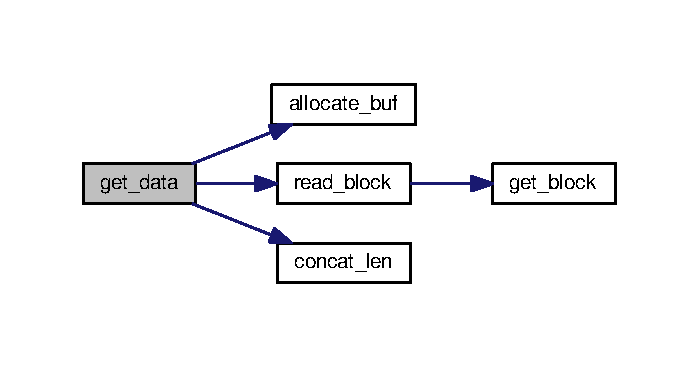
\includegraphics[width=336pt]{block__func_8c_a758063a96fe0be00a4b59b9869a0af62_cgraph}
\end{center}
\end{figure}




Here is the caller graph for this function\-:
\nopagebreak
\begin{figure}[H]
\begin{center}
\leavevmode
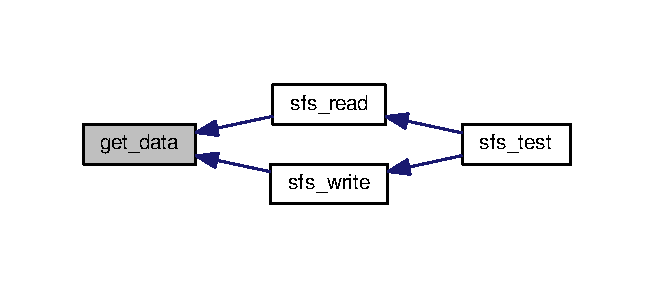
\includegraphics[width=314pt]{block__func_8c_a758063a96fe0be00a4b59b9869a0af62_icgraph}
\end{center}
\end{figure}


\hypertarget{block__func_8c_a1dcadd38a012a1218ab2100bda116861}{\index{block\-\_\-func.\-c@{block\-\_\-func.\-c}!read\-\_\-block@{read\-\_\-block}}
\index{read\-\_\-block@{read\-\_\-block}!block_func.c@{block\-\_\-func.\-c}}
\subsubsection[{read\-\_\-block}]{\setlength{\rightskip}{0pt plus 5cm}int read\-\_\-block (
\begin{DoxyParamCaption}
\item[{uint32\-\_\-t}]{location, }
\item[{{\bf byte} $\ast$}]{buf}
\end{DoxyParamCaption}
)}}\label{block__func_8c_a1dcadd38a012a1218ab2100bda116861}


A wrapper for the get\-\_\-block function. 


\begin{DoxyParams}{Parameters}
{\em location} & The location on disk for the buffer to be written to.\\
\hline
{\em The} & buffer to store on disk.\\
\hline
\end{DoxyParams}
\begin{DoxyReturn}{Returns}
Returns an integer value. If the value $>$= 0 the function was successful. Otherwise, the function was unsuccessful.
\end{DoxyReturn}
\begin{DoxyAuthor}{Author}
Daniel Smullen

Jonathan Gillett

Joseph Heron
\end{DoxyAuthor}
\begin{DoxyCopyright}{Copyright}
G\-N\-U General Public License V3 
\end{DoxyCopyright}


Here is the call graph for this function\-:
\nopagebreak
\begin{figure}[H]
\begin{center}
\leavevmode
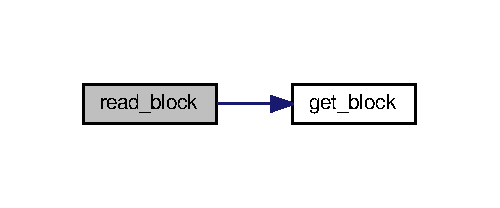
\includegraphics[width=240pt]{block__func_8c_a1dcadd38a012a1218ab2100bda116861_cgraph}
\end{center}
\end{figure}




Here is the caller graph for this function\-:
\nopagebreak
\begin{figure}[H]
\begin{center}
\leavevmode
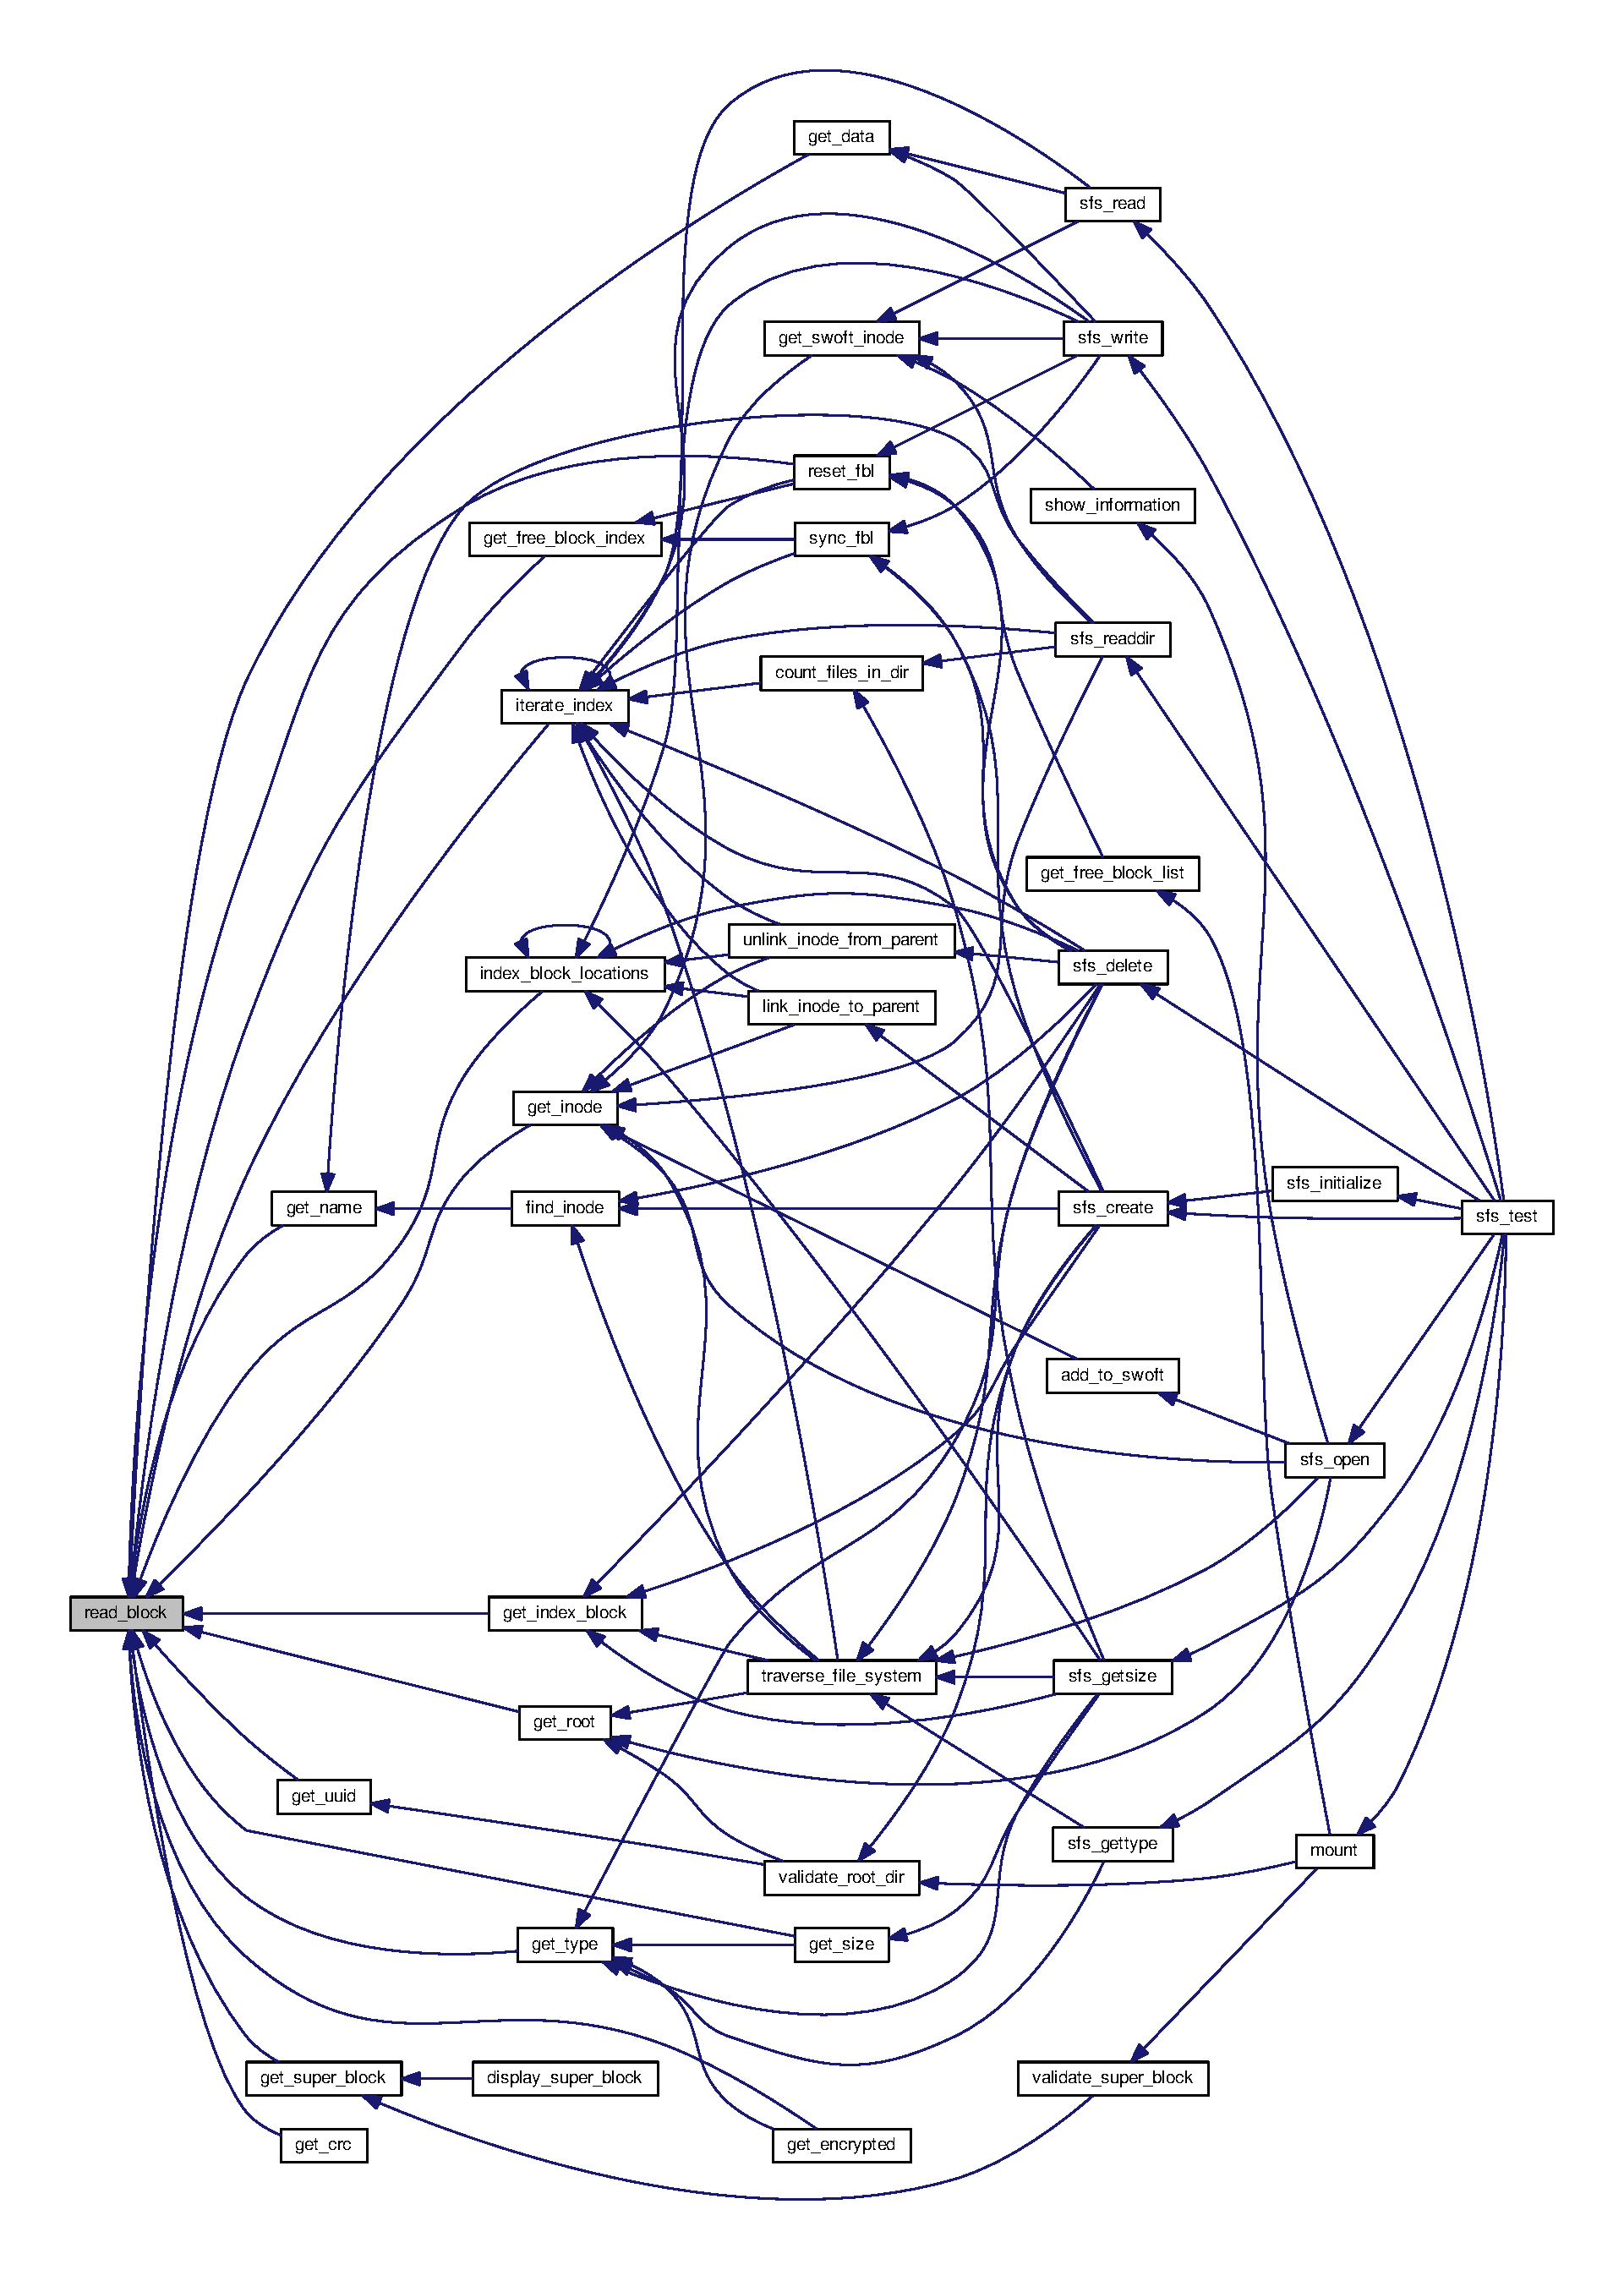
\includegraphics[width=350pt]{block__func_8c_a1dcadd38a012a1218ab2100bda116861_icgraph}
\end{center}
\end{figure}


\hypertarget{block__func_8c_a8d2c516f00e918d009b5fbaf1cfa463b}{\index{block\-\_\-func.\-c@{block\-\_\-func.\-c}!write\-\_\-block@{write\-\_\-block}}
\index{write\-\_\-block@{write\-\_\-block}!block_func.c@{block\-\_\-func.\-c}}
\subsubsection[{write\-\_\-block}]{\setlength{\rightskip}{0pt plus 5cm}int write\-\_\-block (
\begin{DoxyParamCaption}
\item[{uint32\-\_\-t}]{location, }
\item[{{\bf byte} $\ast$}]{buf}
\end{DoxyParamCaption}
)}}\label{block__func_8c_a8d2c516f00e918d009b5fbaf1cfa463b}


A wrapper for the put\-\_\-block function. 


\begin{DoxyParams}{Parameters}
{\em location} & The location on disk for the buffer to be written to.\\
\hline
{\em The} & buffer to store on disk.\\
\hline
\end{DoxyParams}
\begin{DoxyReturn}{Returns}
Returns an integer value. If the value $>$= 0, the function was successful. Otherwise, the function was unsuccessful.
\end{DoxyReturn}
\begin{DoxyAuthor}{Author}
Daniel Smullen

Jonathan Gillett

Joseph Heron
\end{DoxyAuthor}
\begin{DoxyCopyright}{Copyright}
G\-N\-U General Public License V3 
\end{DoxyCopyright}


Here is the call graph for this function\-:
\nopagebreak
\begin{figure}[H]
\begin{center}
\leavevmode
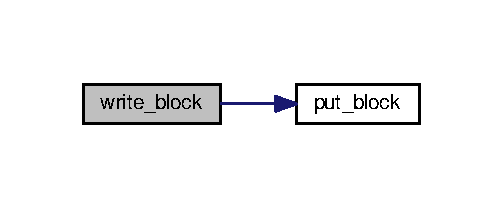
\includegraphics[width=242pt]{block__func_8c_a8d2c516f00e918d009b5fbaf1cfa463b_cgraph}
\end{center}
\end{figure}




Here is the caller graph for this function\-:
\nopagebreak
\begin{figure}[H]
\begin{center}
\leavevmode
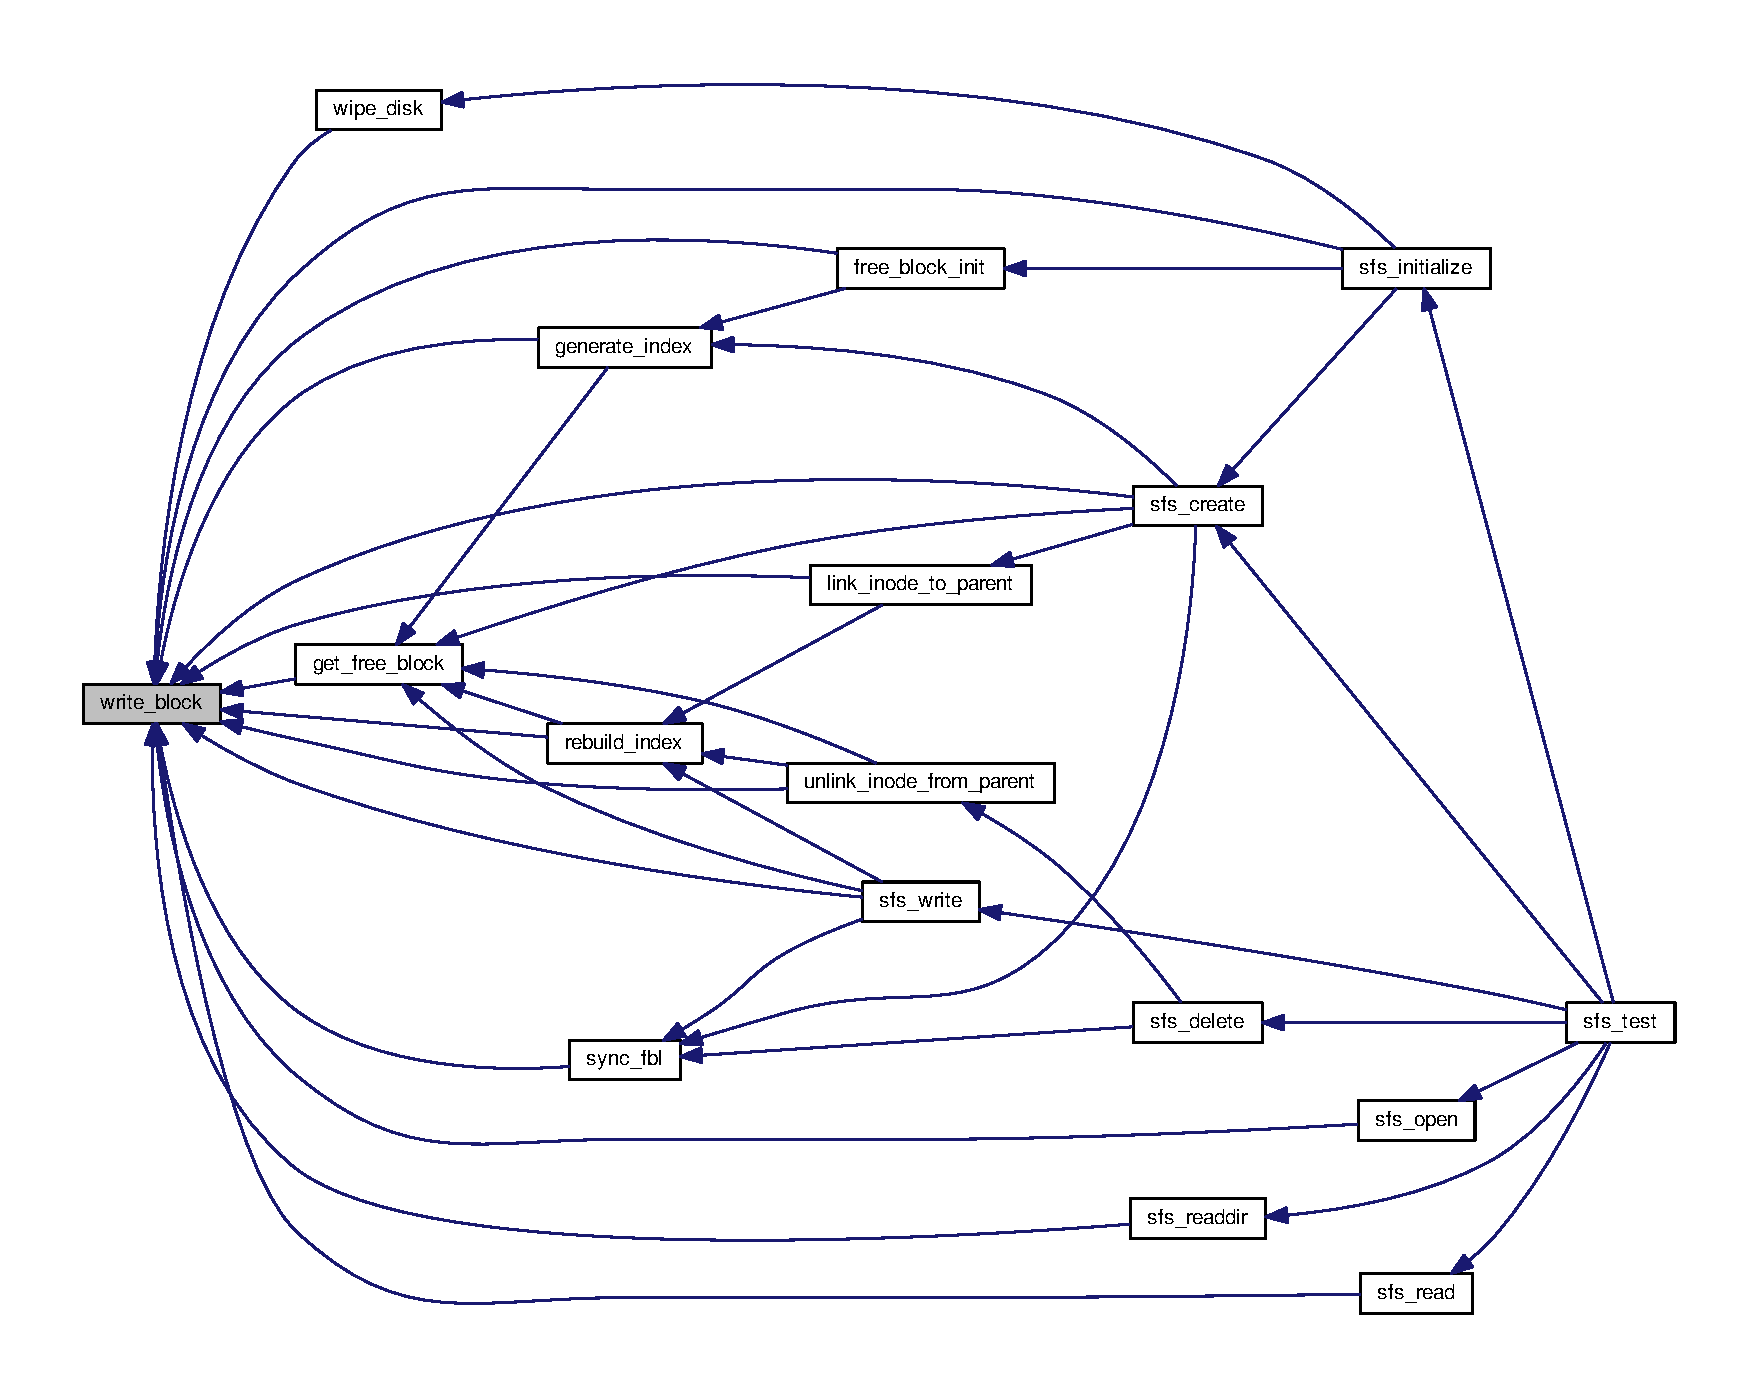
\includegraphics[width=350pt]{block__func_8c_a8d2c516f00e918d009b5fbaf1cfa463b_icgraph}
\end{center}
\end{figure}



\hypertarget{block__func_8h}{\section{block\-\_\-func.\-h File Reference}
\label{block__func_8h}\index{block\-\_\-func.\-h@{block\-\_\-func.\-h}}
}
{\ttfamily \#include \char`\"{}blockio.\-h\char`\"{}}\\*
{\ttfamily \#include \char`\"{}glob\-\_\-data.\-h\char`\"{}}\\*
{\ttfamily \#include \char`\"{}error.\-h\char`\"{}}\\*
Include dependency graph for block\-\_\-func.\-h\-:
\nopagebreak
\begin{figure}[H]
\begin{center}
\leavevmode
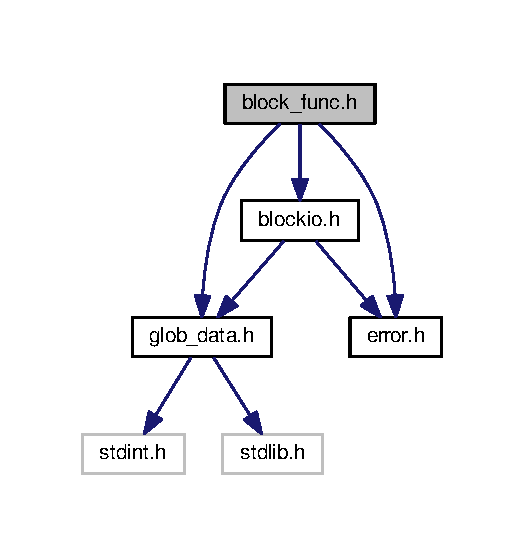
\includegraphics[width=251pt]{block__func_8h__incl}
\end{center}
\end{figure}
This graph shows which files directly or indirectly include this file\-:
\nopagebreak
\begin{figure}[H]
\begin{center}
\leavevmode
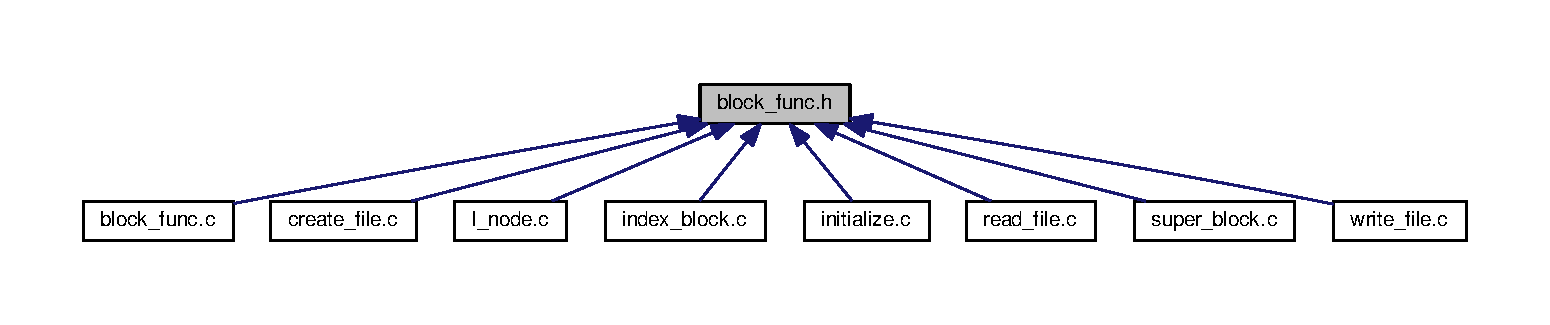
\includegraphics[width=350pt]{block__func_8h__dep__incl}
\end{center}
\end{figure}
\subsection*{Functions}
\begin{DoxyCompactItemize}
\item 
int \hyperlink{block__func_8h_a8d2c516f00e918d009b5fbaf1cfa463b}{write\-\_\-block} (uint32\-\_\-t location, \hyperlink{glob__data_8h_a82b52bf2b45e214a8f2100ebfdf1aee4}{byte} $\ast$buf)
\begin{DoxyCompactList}\small\item\em A wrapper for the put\-\_\-block function. \end{DoxyCompactList}\item 
int \hyperlink{block__func_8h_a1dcadd38a012a1218ab2100bda116861}{read\-\_\-block} (uint32\-\_\-t location, \hyperlink{glob__data_8h_a82b52bf2b45e214a8f2100ebfdf1aee4}{byte} $\ast$buf)
\begin{DoxyCompactList}\small\item\em A wrapper for the get\-\_\-block function. \end{DoxyCompactList}\item 
\hyperlink{glob__data_8h_a82b52bf2b45e214a8f2100ebfdf1aee4}{byte} $\ast$ \hyperlink{block__func_8h_a758063a96fe0be00a4b59b9869a0af62}{get\-\_\-data} (\hyperlink{glob__data_8h_a9d4937e46b9fac69334d5fc7ea3f37a6}{locations} location)
\begin{DoxyCompactList}\small\item\em Get the data blocks and concatenate them into a large byte buffer. \end{DoxyCompactList}\end{DoxyCompactItemize}


\subsection{Function Documentation}
\hypertarget{block__func_8h_a758063a96fe0be00a4b59b9869a0af62}{\index{block\-\_\-func.\-h@{block\-\_\-func.\-h}!get\-\_\-data@{get\-\_\-data}}
\index{get\-\_\-data@{get\-\_\-data}!block_func.h@{block\-\_\-func.\-h}}
\subsubsection[{get\-\_\-data}]{\setlength{\rightskip}{0pt plus 5cm}{\bf byte}$\ast$ get\-\_\-data (
\begin{DoxyParamCaption}
\item[{{\bf locations}}]{location}
\end{DoxyParamCaption}
)}}\label{block__func_8h_a758063a96fe0be00a4b59b9869a0af62}


Get the data blocks and concatenate them into a large byte buffer. 


\begin{DoxyParams}{Parameters}
{\em location} & The locations of the data blocks on disk.\\
\hline
\end{DoxyParams}
\begin{DoxyReturn}{Returns}
Returns the data\-\_\-buffer containing all of the bytes of data.
\end{DoxyReturn}
\begin{DoxyAuthor}{Author}
Daniel Smullen

Jonathan Gillett

Joseph Heron
\end{DoxyAuthor}
\begin{DoxyCopyright}{Copyright}
G\-N\-U General Public License V3 
\end{DoxyCopyright}


Here is the call graph for this function\-:
\nopagebreak
\begin{figure}[H]
\begin{center}
\leavevmode
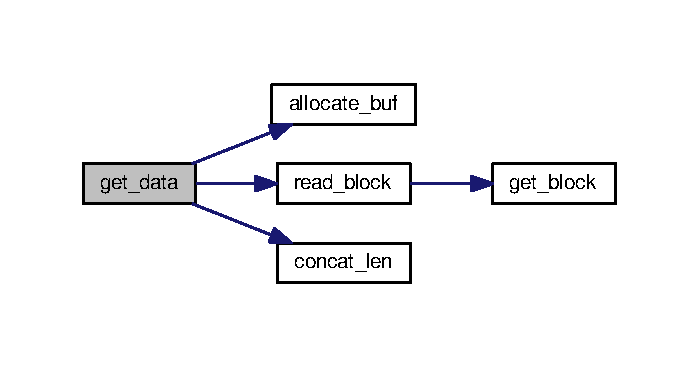
\includegraphics[width=336pt]{block__func_8h_a758063a96fe0be00a4b59b9869a0af62_cgraph}
\end{center}
\end{figure}




Here is the caller graph for this function\-:
\nopagebreak
\begin{figure}[H]
\begin{center}
\leavevmode
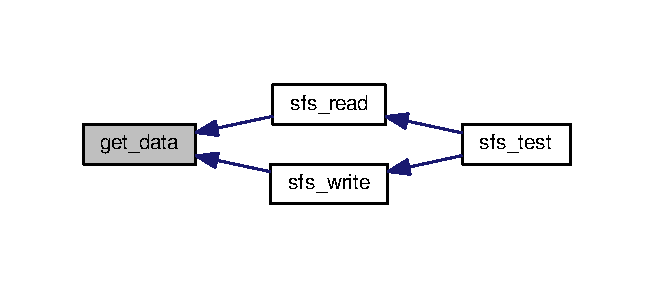
\includegraphics[width=314pt]{block__func_8h_a758063a96fe0be00a4b59b9869a0af62_icgraph}
\end{center}
\end{figure}


\hypertarget{block__func_8h_a1dcadd38a012a1218ab2100bda116861}{\index{block\-\_\-func.\-h@{block\-\_\-func.\-h}!read\-\_\-block@{read\-\_\-block}}
\index{read\-\_\-block@{read\-\_\-block}!block_func.h@{block\-\_\-func.\-h}}
\subsubsection[{read\-\_\-block}]{\setlength{\rightskip}{0pt plus 5cm}int read\-\_\-block (
\begin{DoxyParamCaption}
\item[{uint32\-\_\-t}]{location, }
\item[{{\bf byte} $\ast$}]{buf}
\end{DoxyParamCaption}
)}}\label{block__func_8h_a1dcadd38a012a1218ab2100bda116861}


A wrapper for the get\-\_\-block function. 


\begin{DoxyParams}{Parameters}
{\em location} & The location on disk for the buffer to be written to.\\
\hline
{\em The} & buffer to store on disk.\\
\hline
\end{DoxyParams}
\begin{DoxyReturn}{Returns}
Returns an integer value. If the value $>$= 0 the function was successful. Otherwise, the function was unsuccessful.
\end{DoxyReturn}
\begin{DoxyAuthor}{Author}
Daniel Smullen

Jonathan Gillett

Joseph Heron
\end{DoxyAuthor}
\begin{DoxyCopyright}{Copyright}
G\-N\-U General Public License V3 
\end{DoxyCopyright}


Here is the call graph for this function\-:
\nopagebreak
\begin{figure}[H]
\begin{center}
\leavevmode
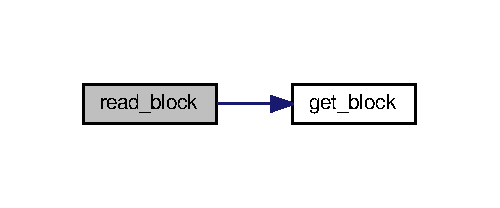
\includegraphics[width=240pt]{block__func_8h_a1dcadd38a012a1218ab2100bda116861_cgraph}
\end{center}
\end{figure}




Here is the caller graph for this function\-:
\nopagebreak
\begin{figure}[H]
\begin{center}
\leavevmode
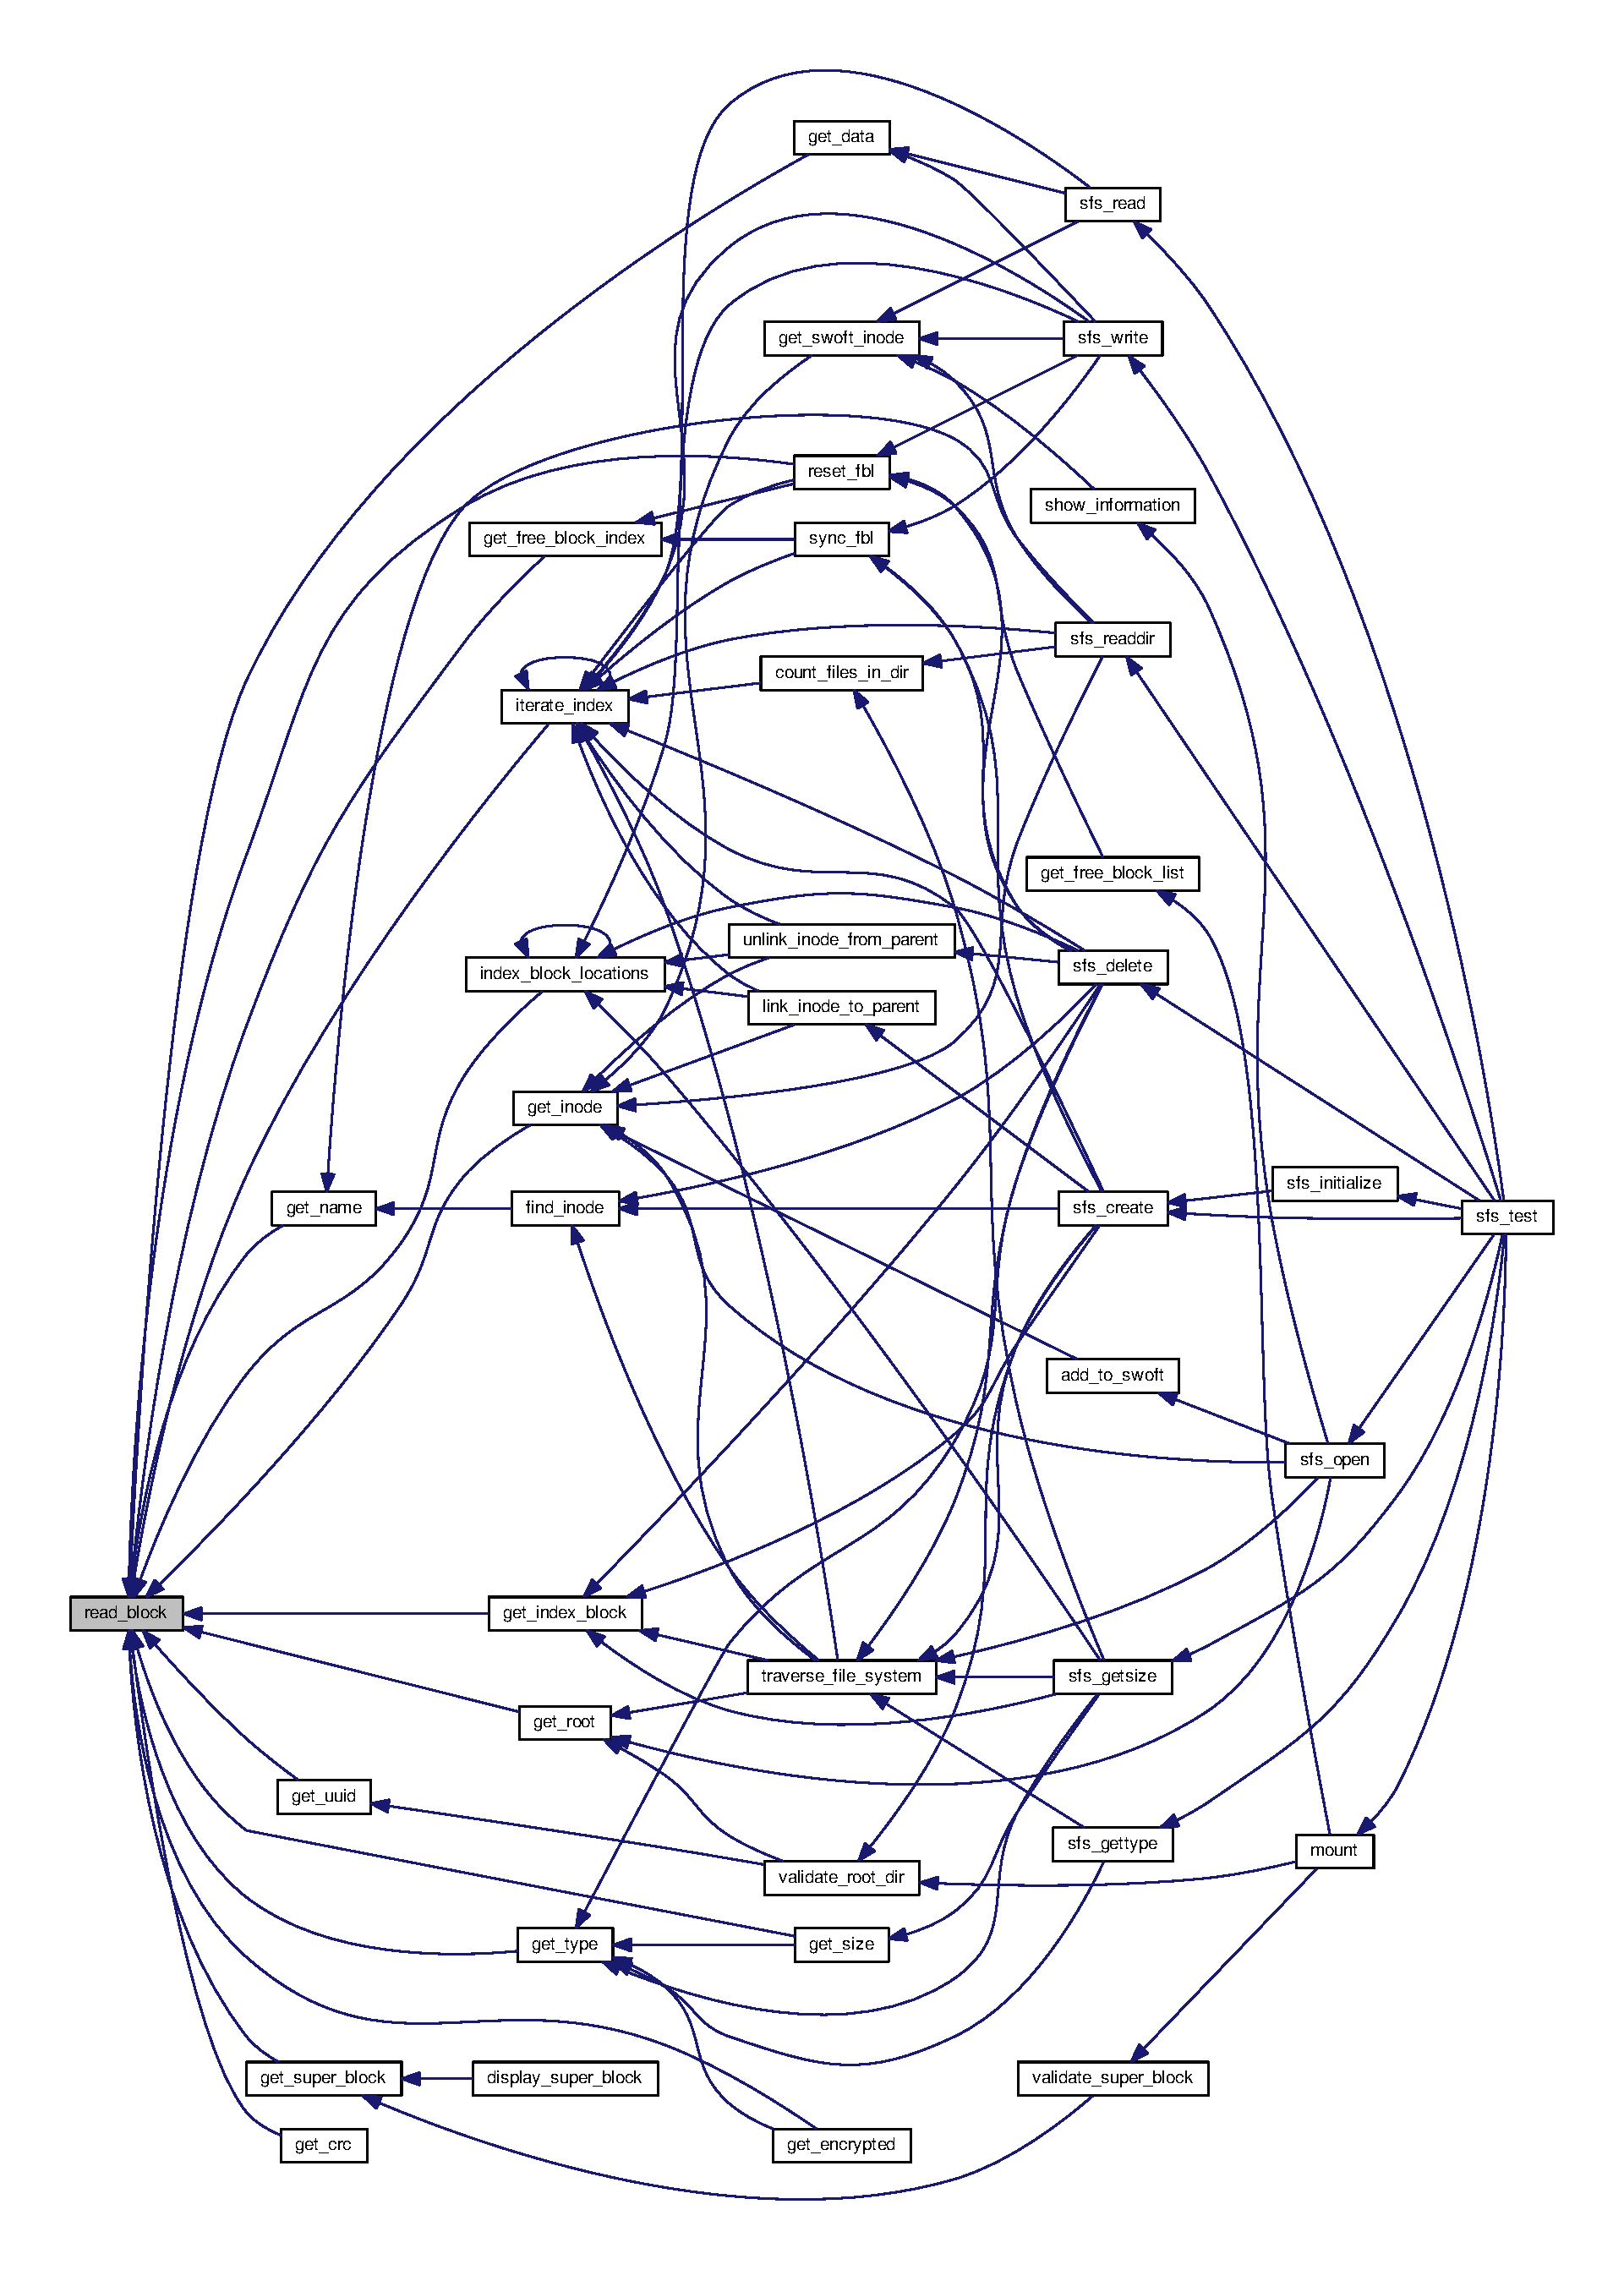
\includegraphics[width=350pt]{block__func_8h_a1dcadd38a012a1218ab2100bda116861_icgraph}
\end{center}
\end{figure}


\hypertarget{block__func_8h_a8d2c516f00e918d009b5fbaf1cfa463b}{\index{block\-\_\-func.\-h@{block\-\_\-func.\-h}!write\-\_\-block@{write\-\_\-block}}
\index{write\-\_\-block@{write\-\_\-block}!block_func.h@{block\-\_\-func.\-h}}
\subsubsection[{write\-\_\-block}]{\setlength{\rightskip}{0pt plus 5cm}int write\-\_\-block (
\begin{DoxyParamCaption}
\item[{uint32\-\_\-t}]{location, }
\item[{{\bf byte} $\ast$}]{buf}
\end{DoxyParamCaption}
)}}\label{block__func_8h_a8d2c516f00e918d009b5fbaf1cfa463b}


A wrapper for the put\-\_\-block function. 


\begin{DoxyParams}{Parameters}
{\em location} & The location on disk for the buffer to be written to.\\
\hline
{\em The} & buffer to store on disk.\\
\hline
\end{DoxyParams}
\begin{DoxyReturn}{Returns}
Returns an integer value. If the value $>$= 0, the function was successful. Otherwise, the function was unsuccessful.
\end{DoxyReturn}
\begin{DoxyAuthor}{Author}
Daniel Smullen

Jonathan Gillett

Joseph Heron
\end{DoxyAuthor}
\begin{DoxyCopyright}{Copyright}
G\-N\-U General Public License V3 
\end{DoxyCopyright}


Here is the call graph for this function\-:
\nopagebreak
\begin{figure}[H]
\begin{center}
\leavevmode
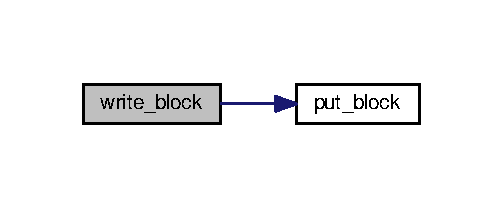
\includegraphics[width=242pt]{block__func_8h_a8d2c516f00e918d009b5fbaf1cfa463b_cgraph}
\end{center}
\end{figure}




Here is the caller graph for this function\-:
\nopagebreak
\begin{figure}[H]
\begin{center}
\leavevmode
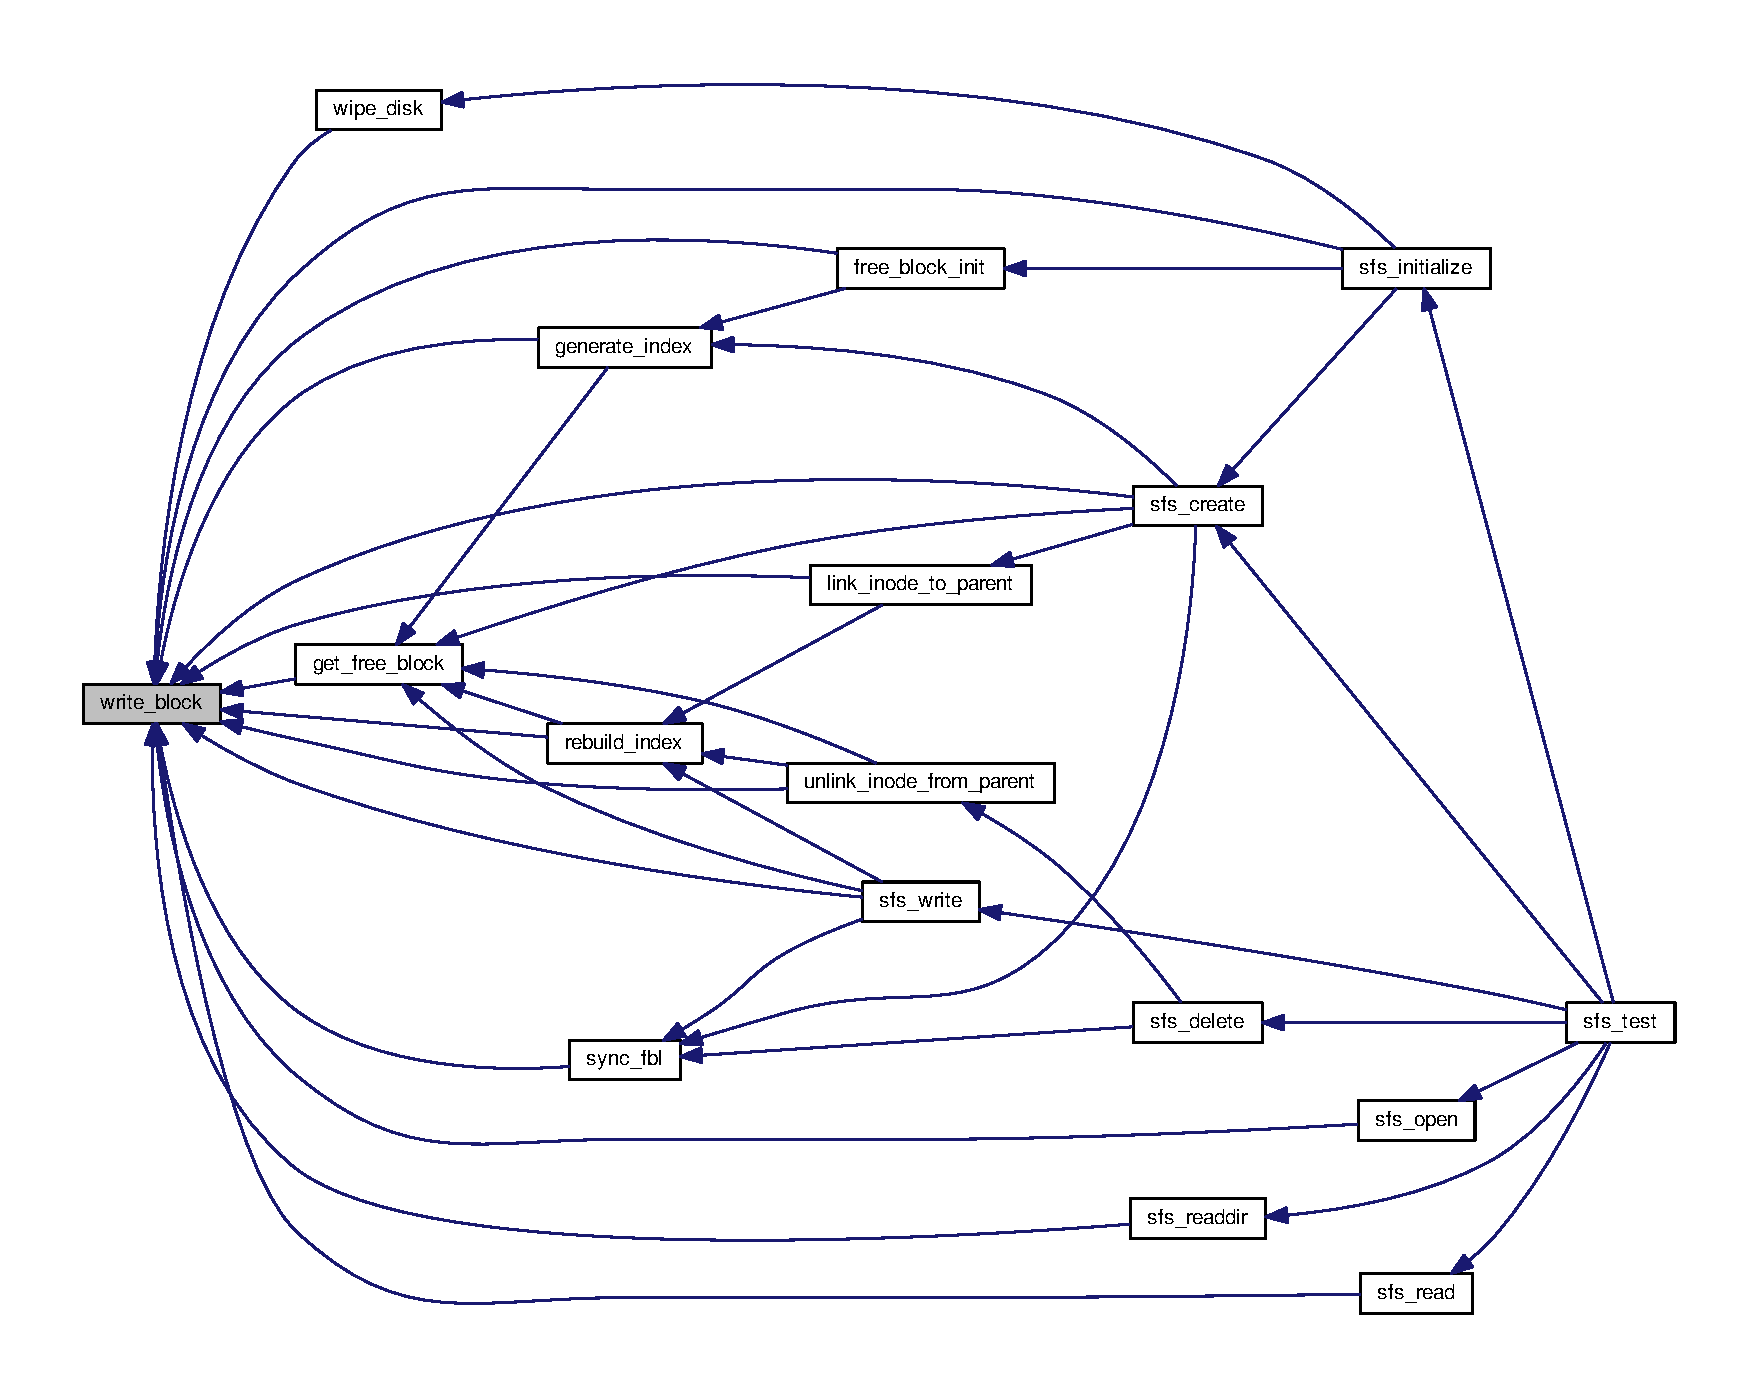
\includegraphics[width=350pt]{block__func_8h_a8d2c516f00e918d009b5fbaf1cfa463b_icgraph}
\end{center}
\end{figure}



\hypertarget{blockio_8c}{\section{blockio.\-c File Reference}
\label{blockio_8c}\index{blockio.\-c@{blockio.\-c}}
}
{\ttfamily \#include $<$sys/types.\-h$>$}\\*
{\ttfamily \#include $<$sys/stat.\-h$>$}\\*
{\ttfamily \#include $<$fcntl.\-h$>$}\\*
{\ttfamily \#include $<$limits.\-h$>$}\\*
{\ttfamily \#include $<$unistd.\-h$>$}\\*
{\ttfamily \#include $<$stdio.\-h$>$}\\*
{\ttfamily \#include \char`\"{}blockio.\-h\char`\"{}}\\*
{\ttfamily \#include \char`\"{}glob\-\_\-data.\-h\char`\"{}}\\*
Include dependency graph for blockio.\-c\-:
\nopagebreak
\begin{figure}[H]
\begin{center}
\leavevmode
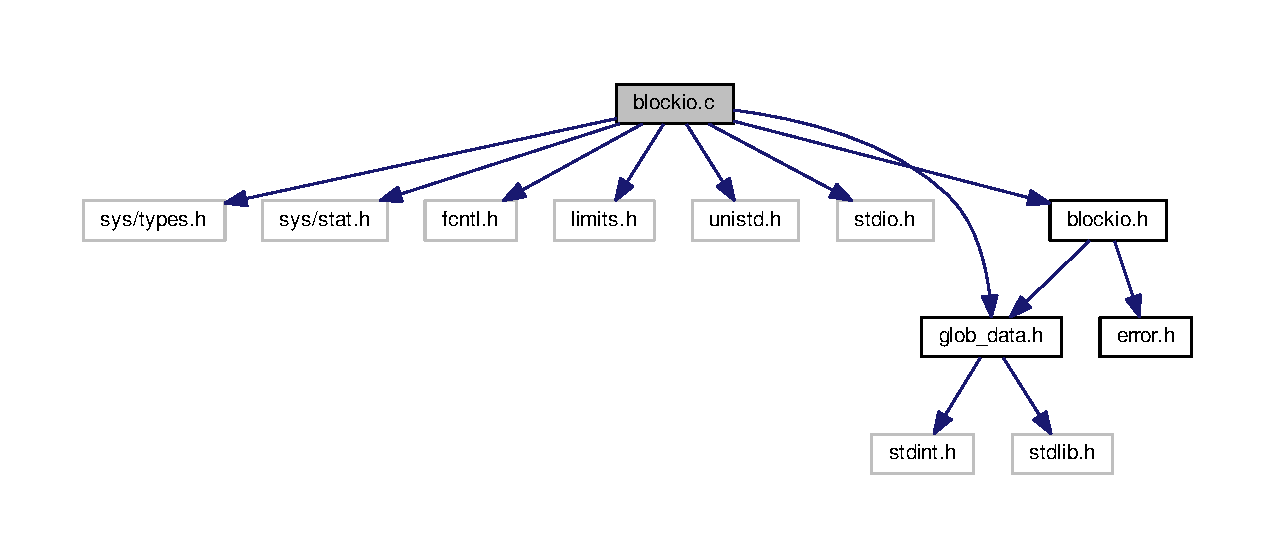
\includegraphics[width=350pt]{blockio_8c__incl}
\end{center}
\end{figure}
\subsection*{Macros}
\begin{DoxyCompactItemize}
\item 
\#define \hyperlink{blockio_8c_a314f278e51bde415c4c5963757cbdcde}{D\-I\-S\-K\-F\-I\-L\-E}~\char`\"{}simdisk.\-data\char`\"{}
\item 
\#define \hyperlink{blockio_8c_a385fbe043a6c0497273f7706486c642b}{D\-I\-S\-K\-F\-I\-L\-E\-M\-O\-D\-E}~S\-\_\-\-I\-R\-U\-S\-R$|$S\-\_\-\-I\-W\-U\-S\-R$|$S\-\_\-\-I\-R\-W\-X\-G
\end{DoxyCompactItemize}
\subsection*{Functions}
\begin{DoxyCompactItemize}
\item 
int \hyperlink{blockio_8c_aba494f8ba12c5888abc3991a9a1a4fa0}{get\-\_\-block} (uint32\-\_\-t blknum, \hyperlink{glob__data_8h_a82b52bf2b45e214a8f2100ebfdf1aee4}{byte} $\ast$buf)
\begin{DoxyCompactList}\small\item\em Retrieves a block from disk. \end{DoxyCompactList}\item 
int \hyperlink{blockio_8c_a800219862241422fe7dee4411b4b995e}{put\-\_\-block} (uint32\-\_\-t blknum, \hyperlink{glob__data_8h_a82b52bf2b45e214a8f2100ebfdf1aee4}{byte} $\ast$buf)
\begin{DoxyCompactList}\small\item\em Writes a block to disk. \end{DoxyCompactList}\end{DoxyCompactItemize}


\subsection{Macro Definition Documentation}
\hypertarget{blockio_8c_a314f278e51bde415c4c5963757cbdcde}{\index{blockio.\-c@{blockio.\-c}!D\-I\-S\-K\-F\-I\-L\-E@{D\-I\-S\-K\-F\-I\-L\-E}}
\index{D\-I\-S\-K\-F\-I\-L\-E@{D\-I\-S\-K\-F\-I\-L\-E}!blockio.c@{blockio.\-c}}
\subsubsection[{D\-I\-S\-K\-F\-I\-L\-E}]{\setlength{\rightskip}{0pt plus 5cm}\#define D\-I\-S\-K\-F\-I\-L\-E~\char`\"{}simdisk.\-data\char`\"{}}}\label{blockio_8c_a314f278e51bde415c4c5963757cbdcde}
\hypertarget{blockio_8c_a385fbe043a6c0497273f7706486c642b}{\index{blockio.\-c@{blockio.\-c}!D\-I\-S\-K\-F\-I\-L\-E\-M\-O\-D\-E@{D\-I\-S\-K\-F\-I\-L\-E\-M\-O\-D\-E}}
\index{D\-I\-S\-K\-F\-I\-L\-E\-M\-O\-D\-E@{D\-I\-S\-K\-F\-I\-L\-E\-M\-O\-D\-E}!blockio.c@{blockio.\-c}}
\subsubsection[{D\-I\-S\-K\-F\-I\-L\-E\-M\-O\-D\-E}]{\setlength{\rightskip}{0pt plus 5cm}\#define D\-I\-S\-K\-F\-I\-L\-E\-M\-O\-D\-E~S\-\_\-\-I\-R\-U\-S\-R$|$S\-\_\-\-I\-W\-U\-S\-R$|$S\-\_\-\-I\-R\-W\-X\-G}}\label{blockio_8c_a385fbe043a6c0497273f7706486c642b}


\subsection{Function Documentation}
\hypertarget{blockio_8c_aba494f8ba12c5888abc3991a9a1a4fa0}{\index{blockio.\-c@{blockio.\-c}!get\-\_\-block@{get\-\_\-block}}
\index{get\-\_\-block@{get\-\_\-block}!blockio.c@{blockio.\-c}}
\subsubsection[{get\-\_\-block}]{\setlength{\rightskip}{0pt plus 5cm}int get\-\_\-block (
\begin{DoxyParamCaption}
\item[{uint32\-\_\-t}]{blknum, }
\item[{{\bf byte} $\ast$}]{buf}
\end{DoxyParamCaption}
)}}\label{blockio_8c_aba494f8ba12c5888abc3991a9a1a4fa0}


Retrieves a block from disk. 


\begin{DoxyParams}{Parameters}
{\em blknum} & Which disk block to retrieve.\\
\hline
{\em buf} & Where in memory to put the retrieved data. \\
\hline
\end{DoxyParams}


Here is the caller graph for this function\-:
\nopagebreak
\begin{figure}[H]
\begin{center}
\leavevmode
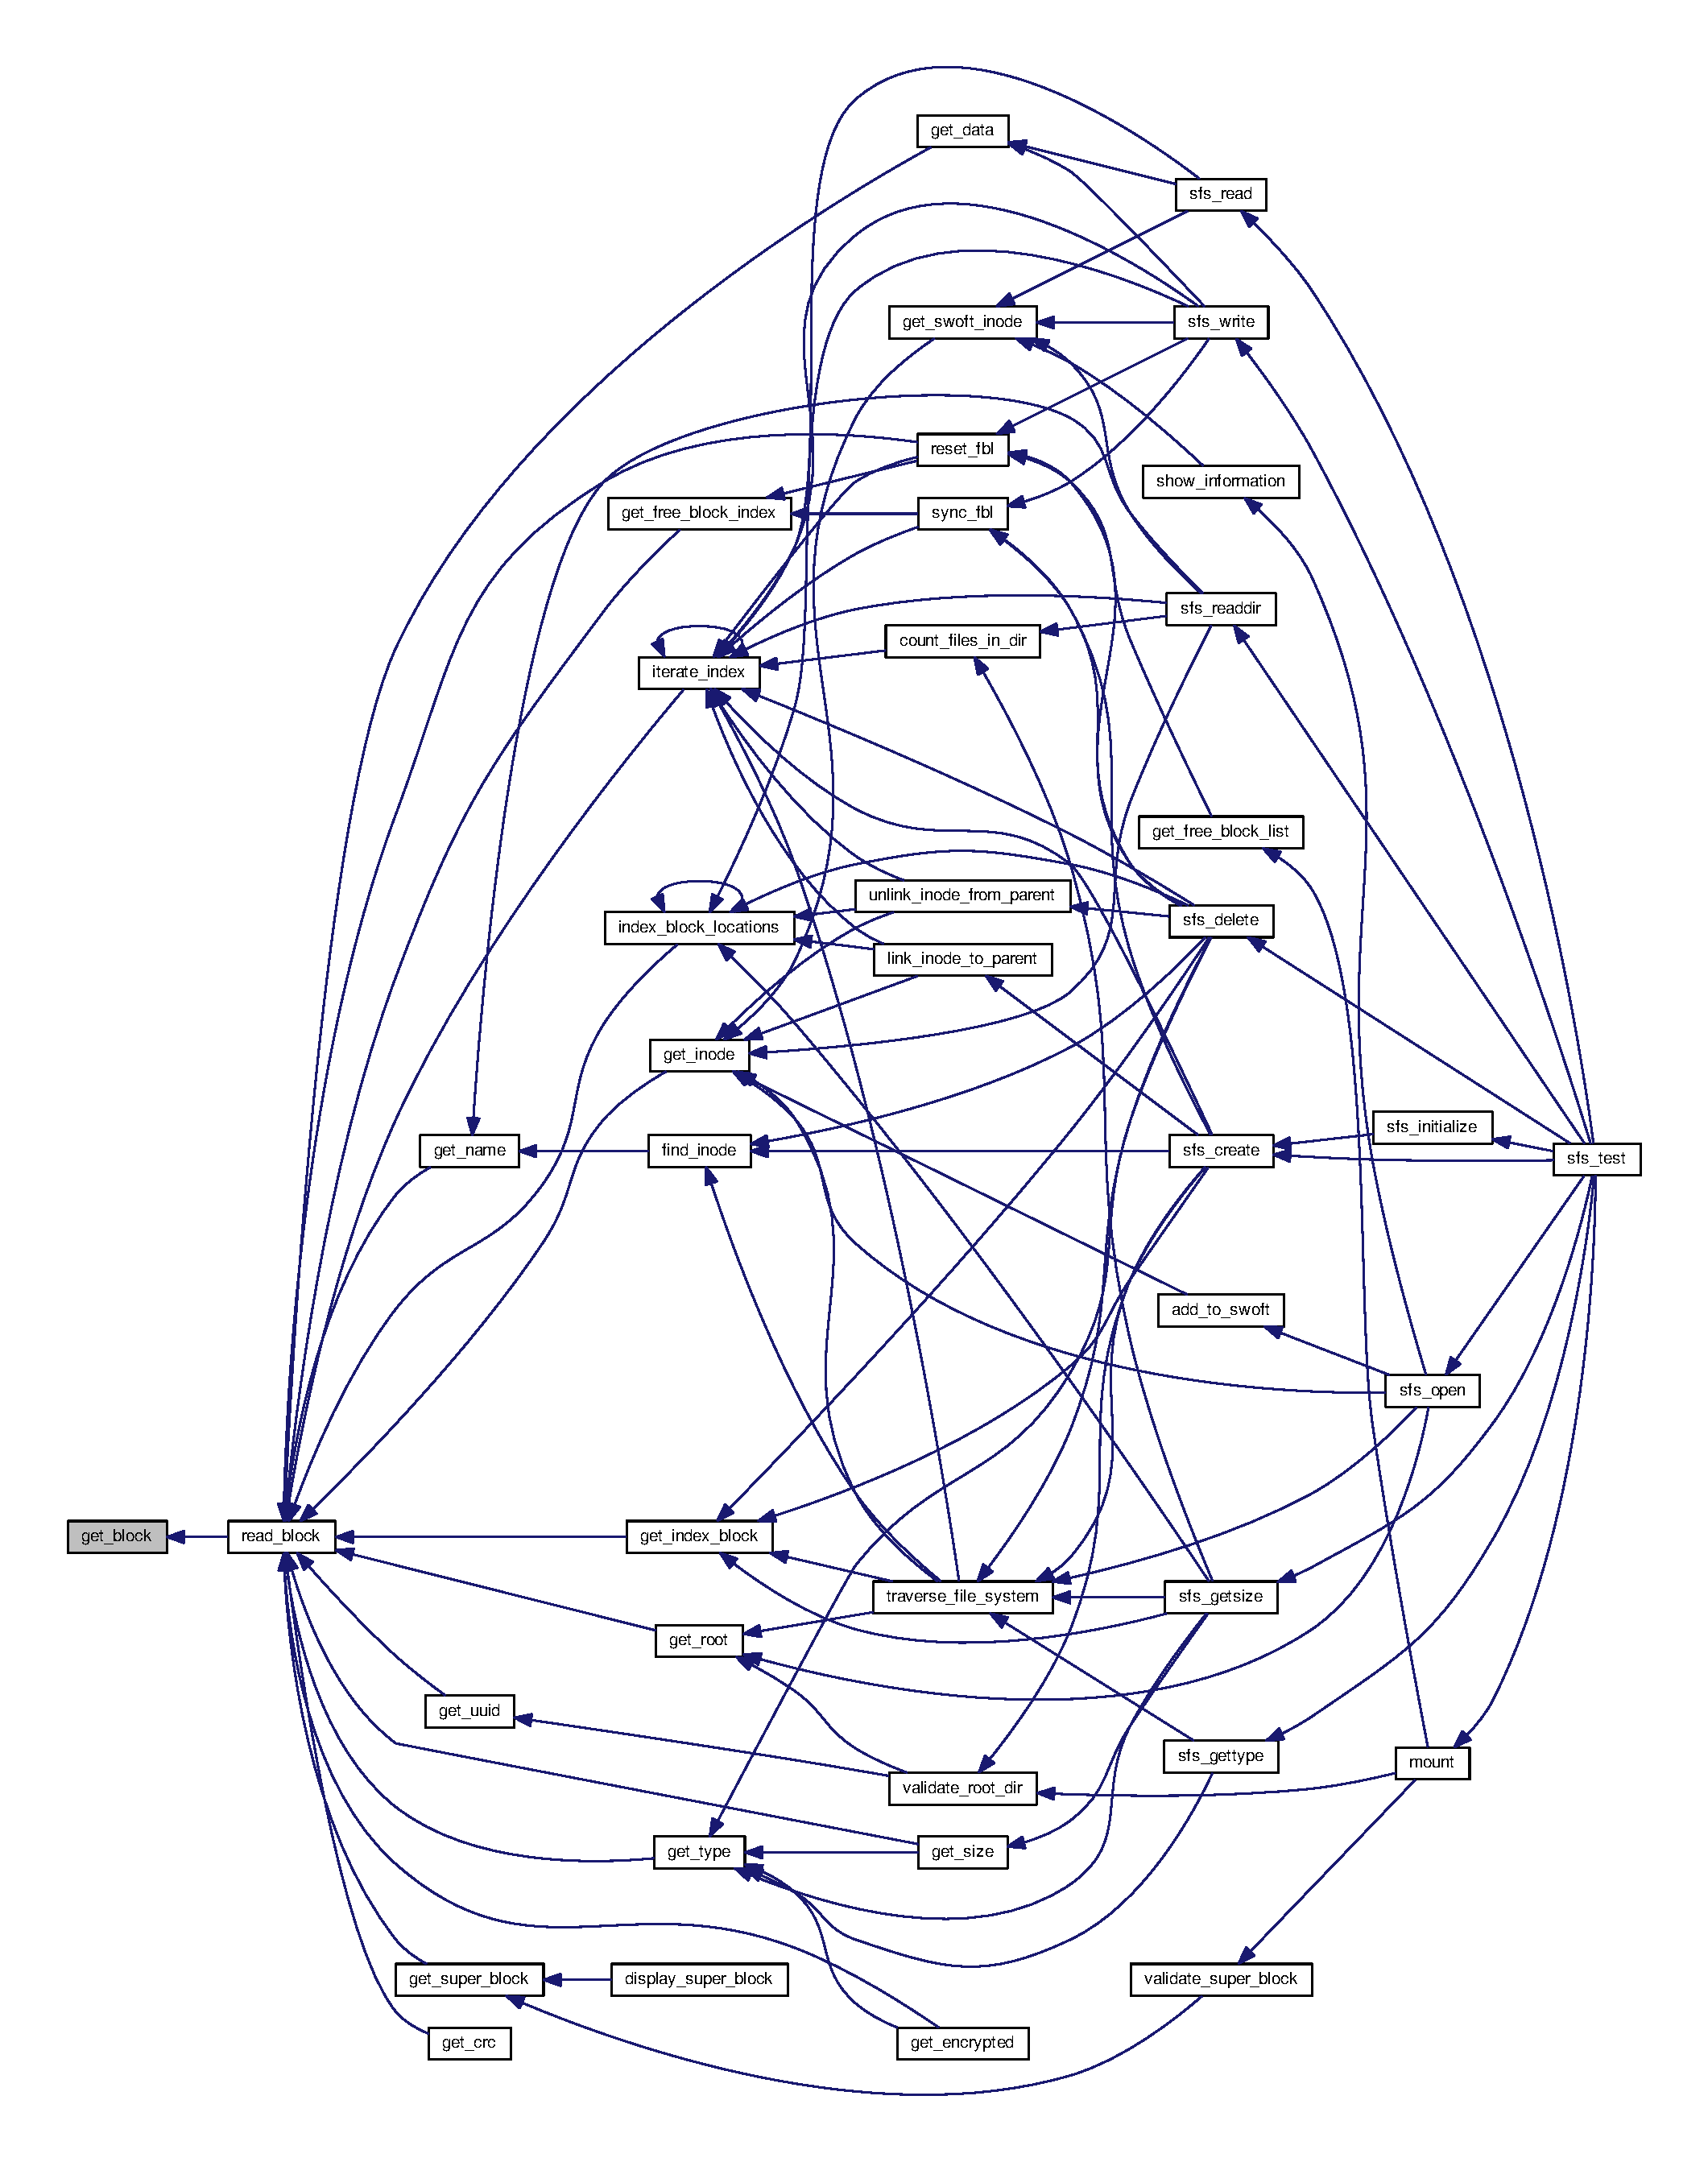
\includegraphics[width=350pt]{blockio_8c_aba494f8ba12c5888abc3991a9a1a4fa0_icgraph}
\end{center}
\end{figure}


\hypertarget{blockio_8c_a800219862241422fe7dee4411b4b995e}{\index{blockio.\-c@{blockio.\-c}!put\-\_\-block@{put\-\_\-block}}
\index{put\-\_\-block@{put\-\_\-block}!blockio.c@{blockio.\-c}}
\subsubsection[{put\-\_\-block}]{\setlength{\rightskip}{0pt plus 5cm}int put\-\_\-block (
\begin{DoxyParamCaption}
\item[{uint32\-\_\-t}]{blknum, }
\item[{{\bf byte} $\ast$}]{buf}
\end{DoxyParamCaption}
)}}\label{blockio_8c_a800219862241422fe7dee4411b4b995e}


Writes a block to disk. 


\begin{DoxyParams}{Parameters}
{\em blknum} & Which disk block to update.\\
\hline
{\em buf} & Where in memory to get new disk block contents. \\
\hline
\end{DoxyParams}


Here is the caller graph for this function\-:
\nopagebreak
\begin{figure}[H]
\begin{center}
\leavevmode
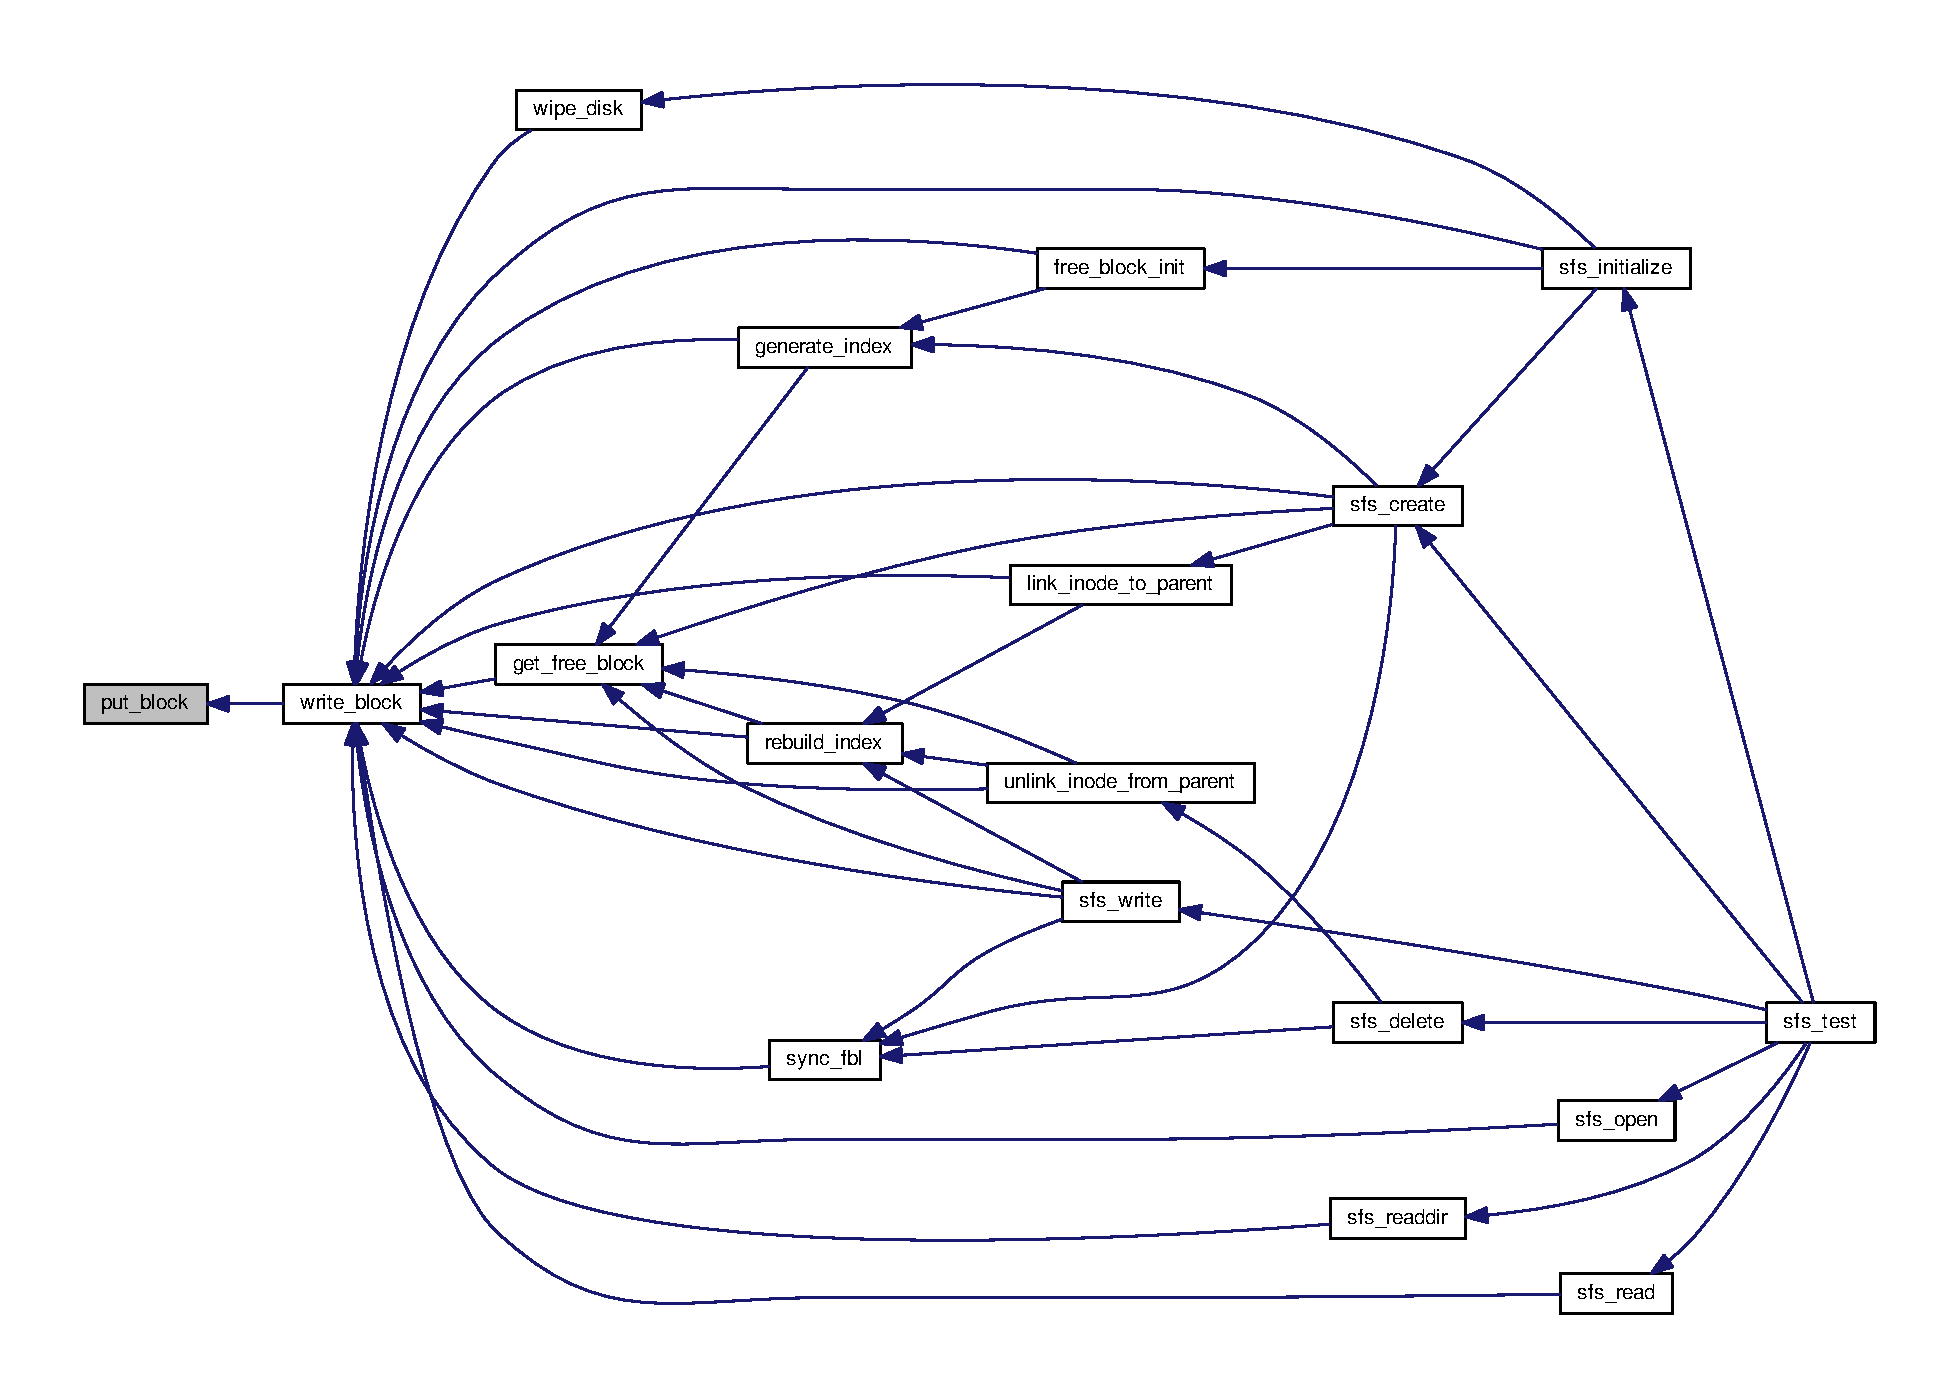
\includegraphics[width=350pt]{blockio_8c_a800219862241422fe7dee4411b4b995e_icgraph}
\end{center}
\end{figure}



\hypertarget{blockio_8h}{\section{blockio.\-h File Reference}
\label{blockio_8h}\index{blockio.\-h@{blockio.\-h}}
}
{\ttfamily \#include \char`\"{}glob\-\_\-data.\-h\char`\"{}}\\*
{\ttfamily \#include \char`\"{}error.\-h\char`\"{}}\\*
Include dependency graph for blockio.\-h\-:
\nopagebreak
\begin{figure}[H]
\begin{center}
\leavevmode
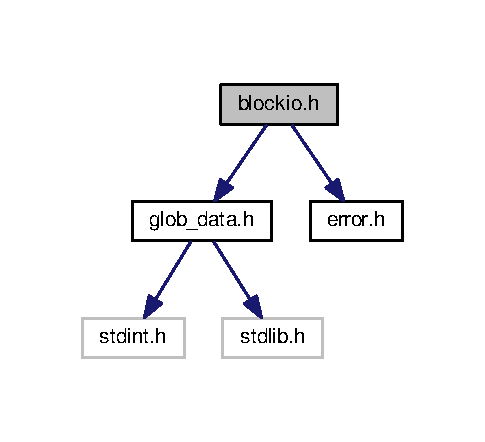
\includegraphics[width=233pt]{blockio_8h__incl}
\end{center}
\end{figure}
This graph shows which files directly or indirectly include this file\-:
\nopagebreak
\begin{figure}[H]
\begin{center}
\leavevmode
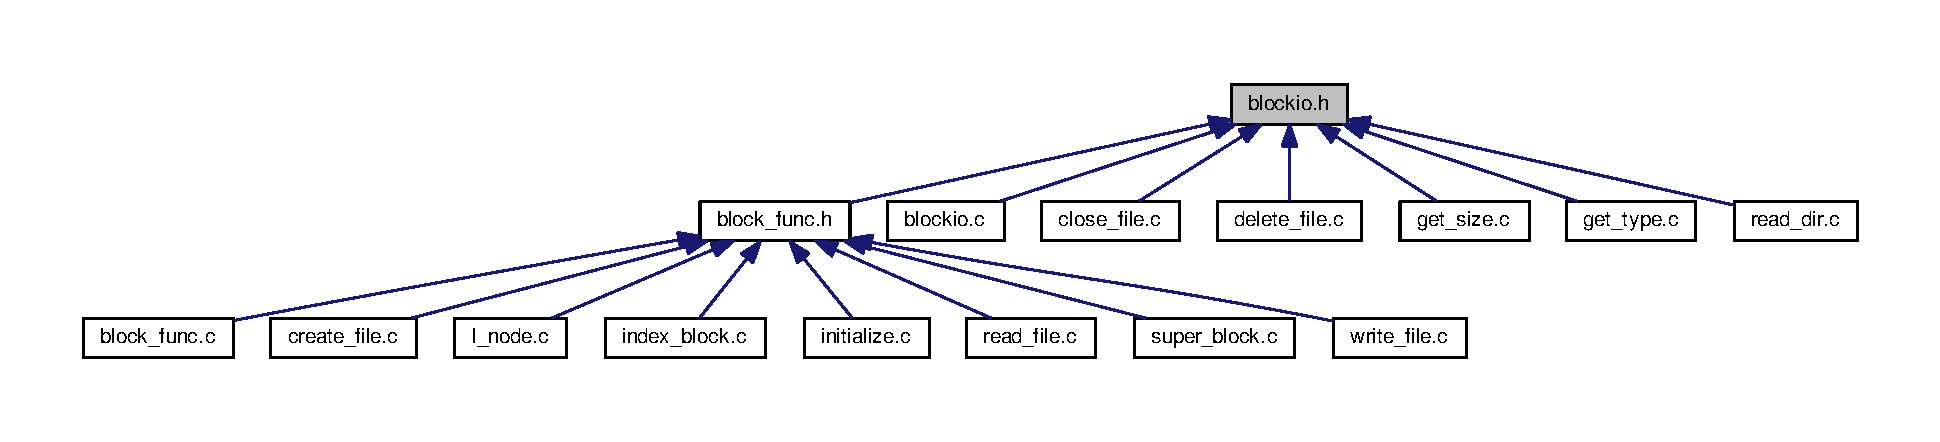
\includegraphics[width=350pt]{blockio_8h__dep__incl}
\end{center}
\end{figure}
\subsection*{Functions}
\begin{DoxyCompactItemize}
\item 
int \hyperlink{blockio_8h_aba494f8ba12c5888abc3991a9a1a4fa0}{get\-\_\-block} (uint32\-\_\-t blknum, \hyperlink{glob__data_8h_a82b52bf2b45e214a8f2100ebfdf1aee4}{byte} $\ast$buf)
\begin{DoxyCompactList}\small\item\em Retrieves a block from disk. \end{DoxyCompactList}\item 
int \hyperlink{blockio_8h_a800219862241422fe7dee4411b4b995e}{put\-\_\-block} (uint32\-\_\-t blknum, \hyperlink{glob__data_8h_a82b52bf2b45e214a8f2100ebfdf1aee4}{byte} $\ast$buf)
\begin{DoxyCompactList}\small\item\em Writes a block to disk. \end{DoxyCompactList}\end{DoxyCompactItemize}


\subsection{Function Documentation}
\hypertarget{blockio_8h_aba494f8ba12c5888abc3991a9a1a4fa0}{\index{blockio.\-h@{blockio.\-h}!get\-\_\-block@{get\-\_\-block}}
\index{get\-\_\-block@{get\-\_\-block}!blockio.h@{blockio.\-h}}
\subsubsection[{get\-\_\-block}]{\setlength{\rightskip}{0pt plus 5cm}int get\-\_\-block (
\begin{DoxyParamCaption}
\item[{uint32\-\_\-t}]{blknum, }
\item[{{\bf byte} $\ast$}]{buf}
\end{DoxyParamCaption}
)}}\label{blockio_8h_aba494f8ba12c5888abc3991a9a1a4fa0}


Retrieves a block from disk. 


\begin{DoxyParams}{Parameters}
{\em blknum} & Which disk block to retrieve.\\
\hline
{\em buf} & Where in memory to put the retrieved data. \\
\hline
\end{DoxyParams}


Here is the caller graph for this function\-:
\nopagebreak
\begin{figure}[H]
\begin{center}
\leavevmode
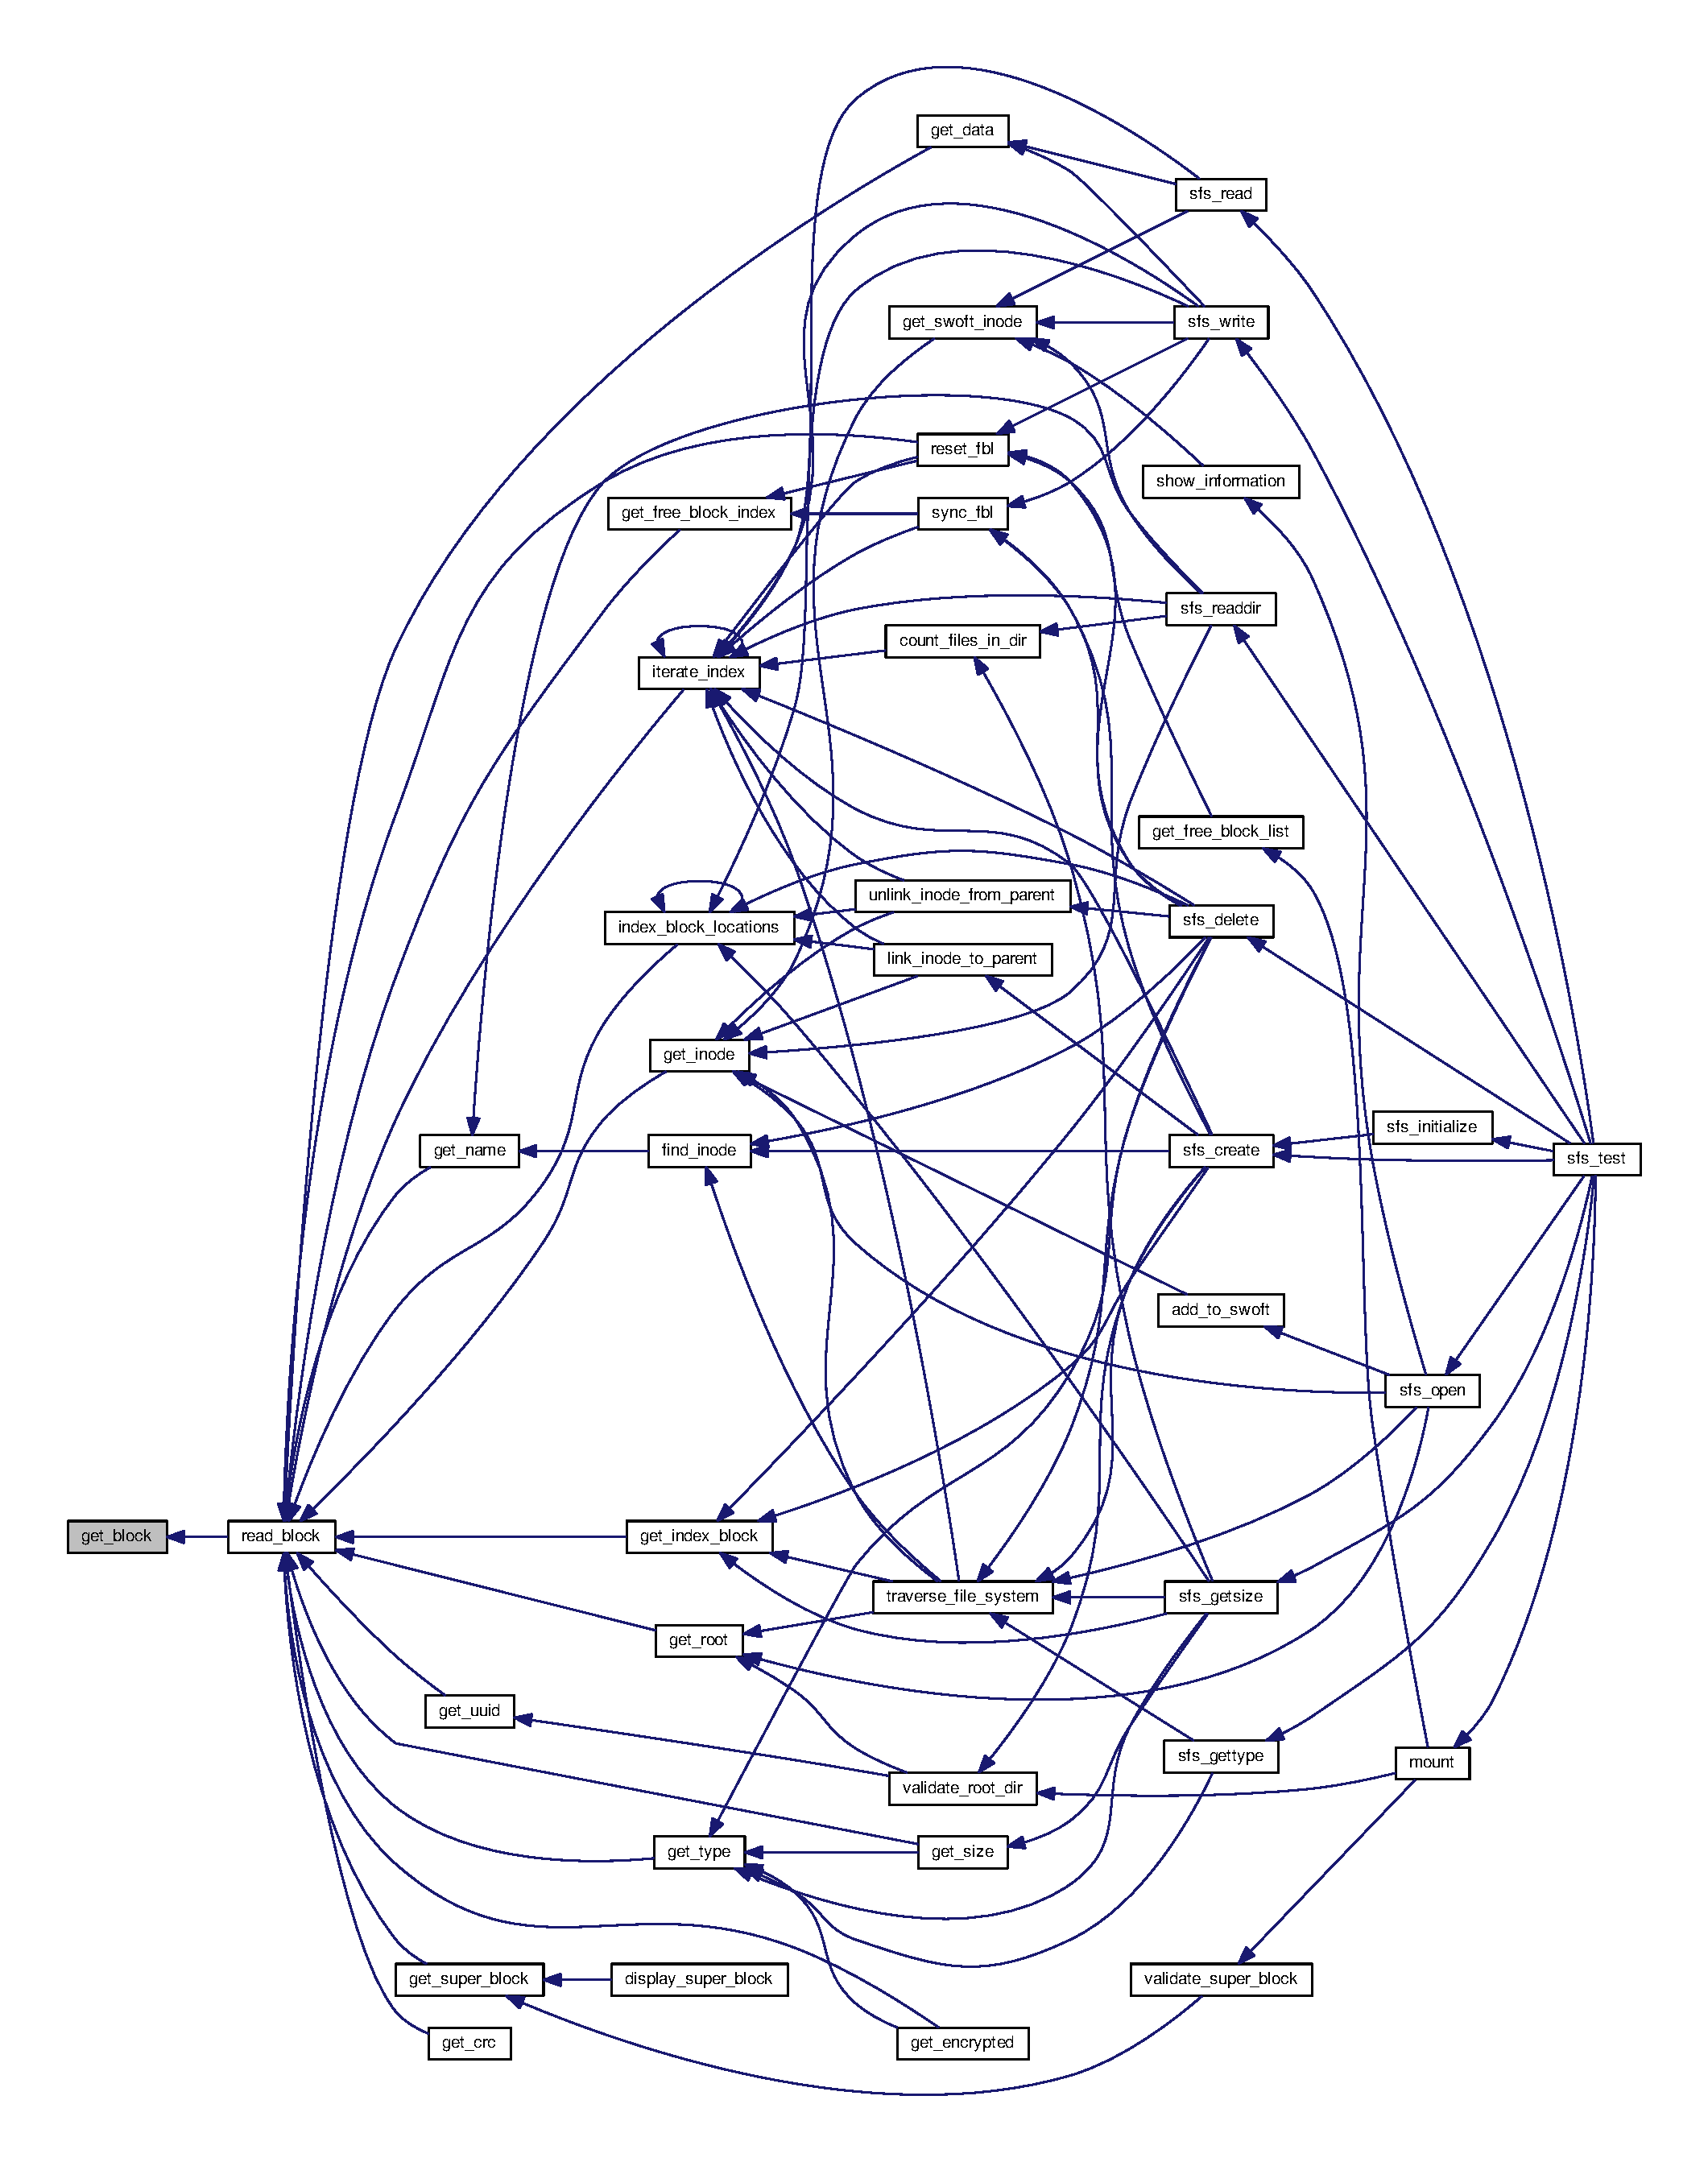
\includegraphics[width=350pt]{blockio_8h_aba494f8ba12c5888abc3991a9a1a4fa0_icgraph}
\end{center}
\end{figure}


\hypertarget{blockio_8h_a800219862241422fe7dee4411b4b995e}{\index{blockio.\-h@{blockio.\-h}!put\-\_\-block@{put\-\_\-block}}
\index{put\-\_\-block@{put\-\_\-block}!blockio.h@{blockio.\-h}}
\subsubsection[{put\-\_\-block}]{\setlength{\rightskip}{0pt plus 5cm}int put\-\_\-block (
\begin{DoxyParamCaption}
\item[{uint32\-\_\-t}]{blknum, }
\item[{{\bf byte} $\ast$}]{buf}
\end{DoxyParamCaption}
)}}\label{blockio_8h_a800219862241422fe7dee4411b4b995e}


Writes a block to disk. 


\begin{DoxyParams}{Parameters}
{\em blknum} & Which disk block to update.\\
\hline
{\em buf} & Where in memory to get new disk block contents. \\
\hline
\end{DoxyParams}


Here is the caller graph for this function\-:
\nopagebreak
\begin{figure}[H]
\begin{center}
\leavevmode
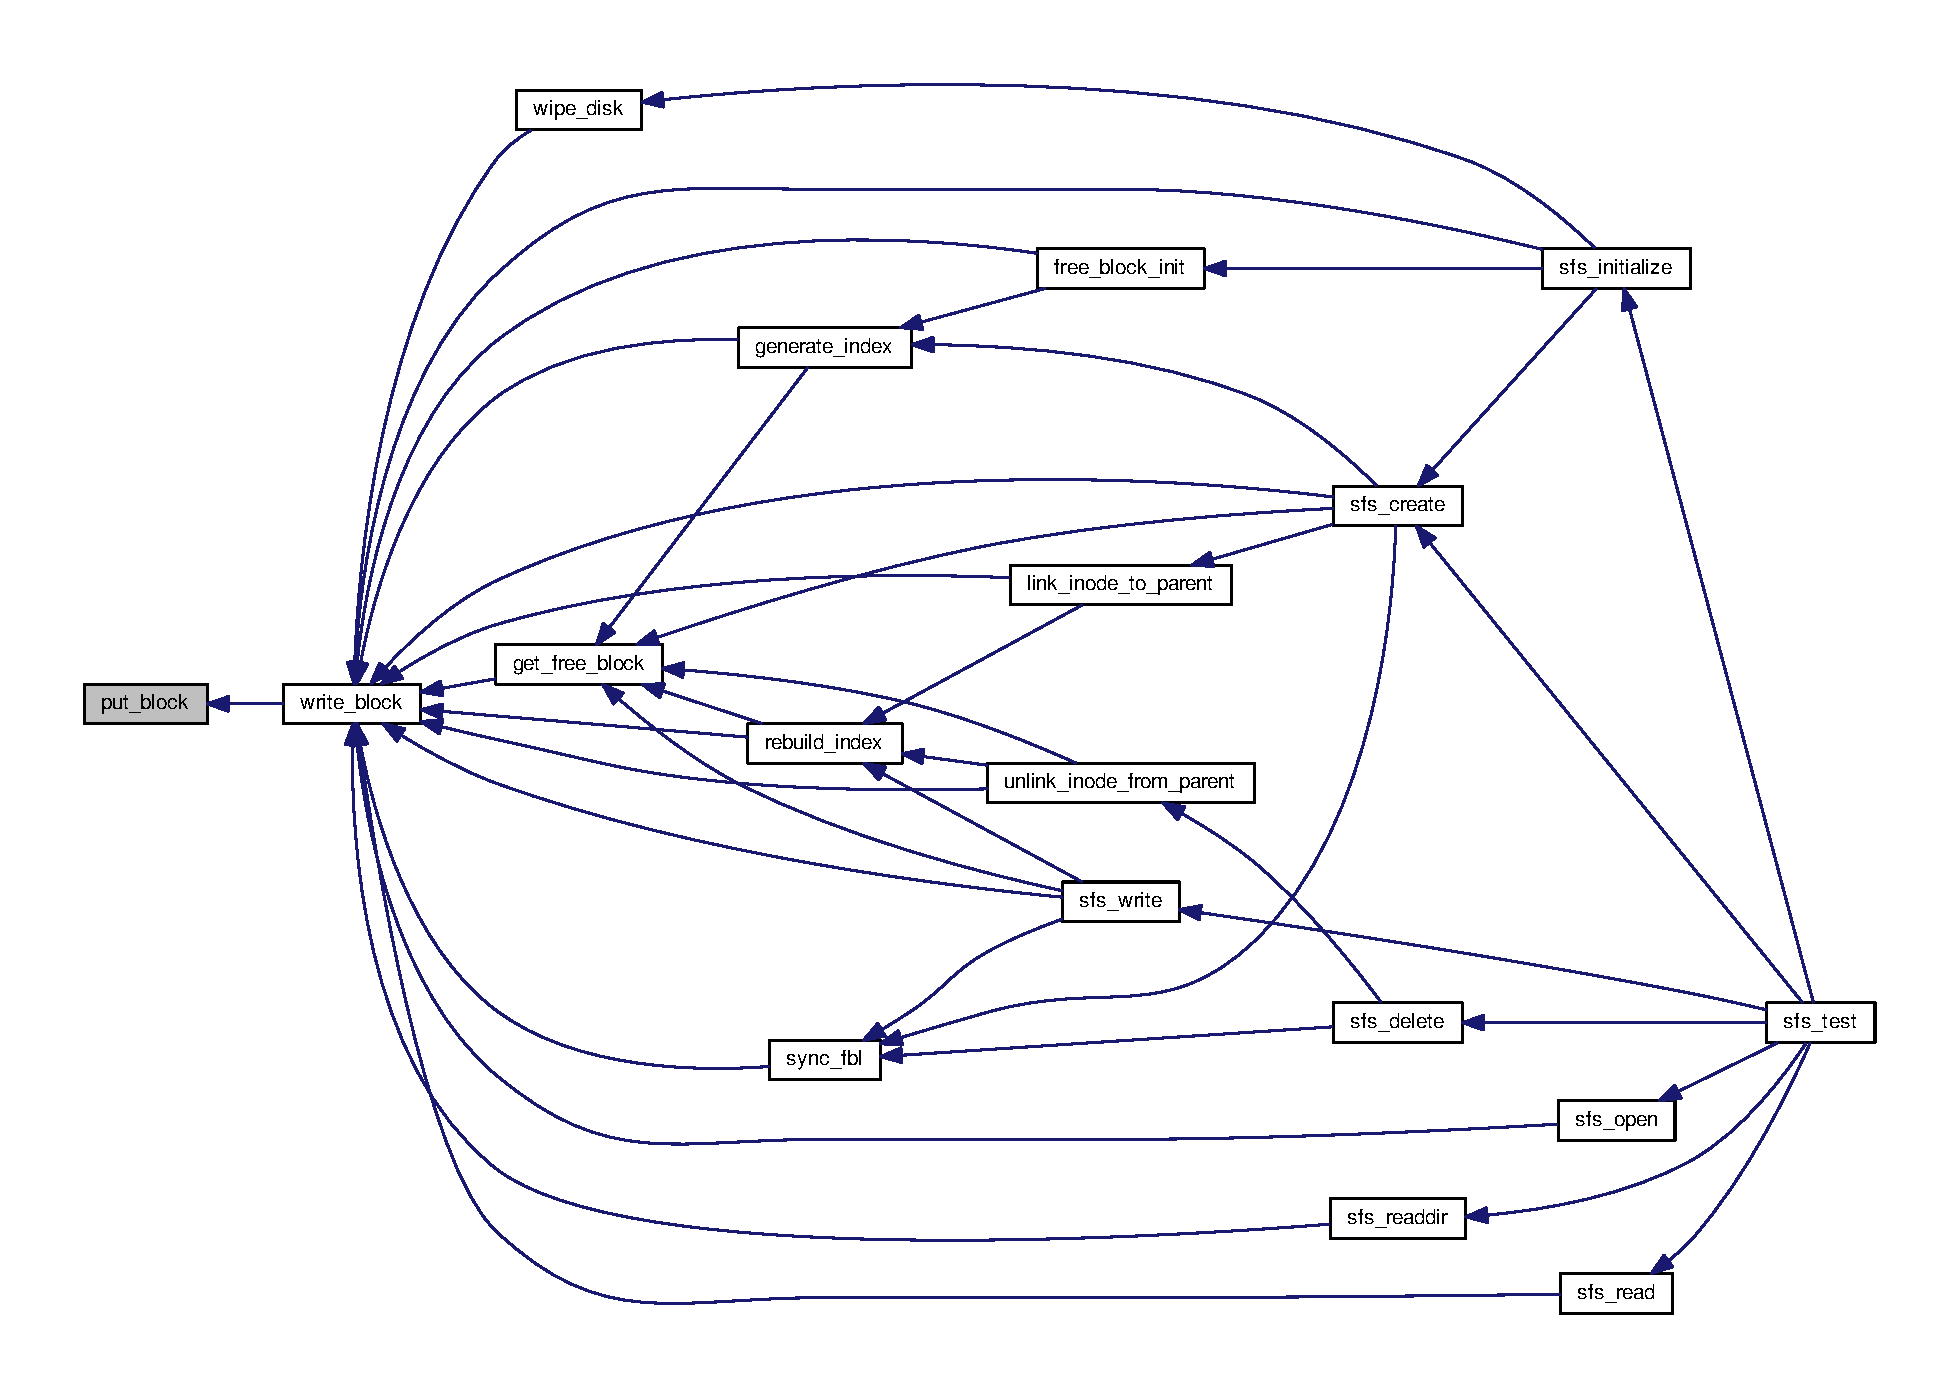
\includegraphics[width=350pt]{blockio_8h_a800219862241422fe7dee4411b4b995e_icgraph}
\end{center}
\end{figure}



\hypertarget{close__file_8c}{\section{close\-\_\-file.\-c File Reference}
\label{close__file_8c}\index{close\-\_\-file.\-c@{close\-\_\-file.\-c}}
}
{\ttfamily \#include \char`\"{}blockio.\-h\char`\"{}}\\*
{\ttfamily \#include \char`\"{}close\-\_\-file.\-h\char`\"{}}\\*
Include dependency graph for close\-\_\-file.\-c\-:
\nopagebreak
\begin{figure}[H]
\begin{center}
\leavevmode
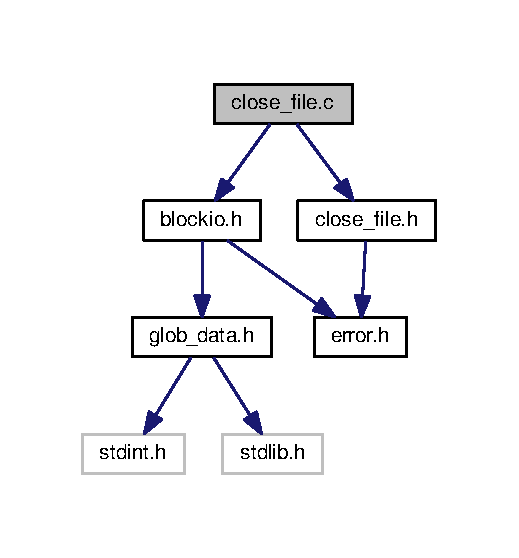
\includegraphics[width=249pt]{close__file_8c__incl}
\end{center}
\end{figure}
\subsection*{Functions}
\begin{DoxyCompactItemize}
\item 
int \hyperlink{close__file_8c_ab89c6dcbc639c5fb3348a6935c12912d}{sfs\-\_\-close} (int fd)
\begin{DoxyCompactList}\small\item\em Closes the file, which indicates that the file is no longer needed. \end{DoxyCompactList}\end{DoxyCompactItemize}


\subsection{Function Documentation}
\hypertarget{close__file_8c_ab89c6dcbc639c5fb3348a6935c12912d}{\index{close\-\_\-file.\-c@{close\-\_\-file.\-c}!sfs\-\_\-close@{sfs\-\_\-close}}
\index{sfs\-\_\-close@{sfs\-\_\-close}!close_file.c@{close\-\_\-file.\-c}}
\subsubsection[{sfs\-\_\-close}]{\setlength{\rightskip}{0pt plus 5cm}int sfs\-\_\-close (
\begin{DoxyParamCaption}
\item[{int}]{fd}
\end{DoxyParamCaption}
)}}\label{close__file_8c_ab89c6dcbc639c5fb3348a6935c12912d}


Closes the file, which indicates that the file is no longer needed. 


\begin{DoxyParams}{Parameters}
{\em fd} & A file descriptor for the file to close.\\
\hline
\end{DoxyParams}
\begin{DoxyReturn}{Returns}
Returns an integer value. If the value is $>$ 0 the file close was a success, if the value $<$= 0 the file close was unsuccessful.
\end{DoxyReturn}
\begin{DoxyAuthor}{Author}
Daniel Smullen

Jonathan Gillett

Joseph Heron
\end{DoxyAuthor}
\begin{DoxyCopyright}{Copyright}
G\-N\-U General Public License V3 
\end{DoxyCopyright}


Here is the call graph for this function\-:
\nopagebreak
\begin{figure}[H]
\begin{center}
\leavevmode
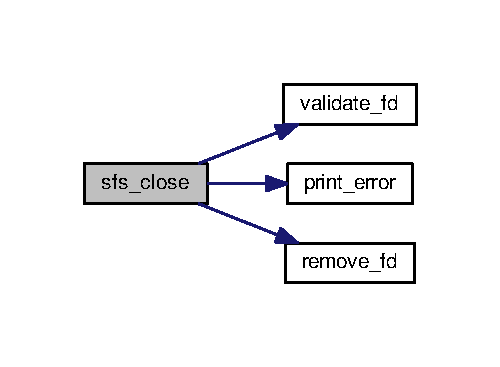
\includegraphics[width=240pt]{close__file_8c_ab89c6dcbc639c5fb3348a6935c12912d_cgraph}
\end{center}
\end{figure}




Here is the caller graph for this function\-:
\nopagebreak
\begin{figure}[H]
\begin{center}
\leavevmode
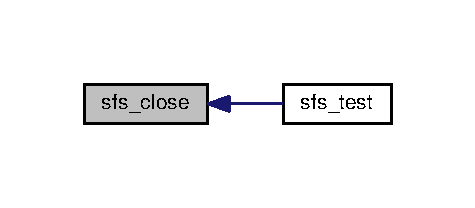
\includegraphics[width=228pt]{close__file_8c_ab89c6dcbc639c5fb3348a6935c12912d_icgraph}
\end{center}
\end{figure}



\hypertarget{close__file_8h}{\section{close\-\_\-file.\-h File Reference}
\label{close__file_8h}\index{close\-\_\-file.\-h@{close\-\_\-file.\-h}}
}
{\ttfamily \#include \char`\"{}error.\-h\char`\"{}}\\*
Include dependency graph for close\-\_\-file.\-h\-:
\nopagebreak
\begin{figure}[H]
\begin{center}
\leavevmode
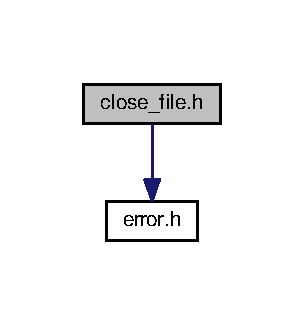
\includegraphics[width=146pt]{close__file_8h__incl}
\end{center}
\end{figure}
This graph shows which files directly or indirectly include this file\-:
\nopagebreak
\begin{figure}[H]
\begin{center}
\leavevmode
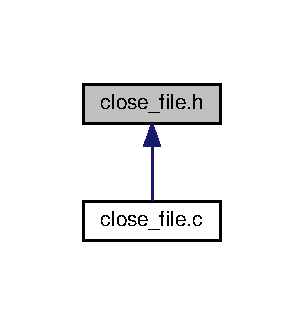
\includegraphics[width=146pt]{close__file_8h__dep__incl}
\end{center}
\end{figure}
\subsection*{Functions}
\begin{DoxyCompactItemize}
\item 
int \hyperlink{close__file_8h_ab89c6dcbc639c5fb3348a6935c12912d}{sfs\-\_\-close} (int fd)
\begin{DoxyCompactList}\small\item\em Closes the file, which indicates that the file is no longer needed. \end{DoxyCompactList}\end{DoxyCompactItemize}


\subsection{Function Documentation}
\hypertarget{close__file_8h_ab89c6dcbc639c5fb3348a6935c12912d}{\index{close\-\_\-file.\-h@{close\-\_\-file.\-h}!sfs\-\_\-close@{sfs\-\_\-close}}
\index{sfs\-\_\-close@{sfs\-\_\-close}!close_file.h@{close\-\_\-file.\-h}}
\subsubsection[{sfs\-\_\-close}]{\setlength{\rightskip}{0pt plus 5cm}int sfs\-\_\-close (
\begin{DoxyParamCaption}
\item[{int}]{fd}
\end{DoxyParamCaption}
)}}\label{close__file_8h_ab89c6dcbc639c5fb3348a6935c12912d}


Closes the file, which indicates that the file is no longer needed. 


\begin{DoxyParams}{Parameters}
{\em fd} & A file descriptor for the file to close.\\
\hline
\end{DoxyParams}
\begin{DoxyReturn}{Returns}
Returns an integer value. If the value is $>$ 0 the file close was a success, if the value $<$= 0 the file close was unsuccessful.
\end{DoxyReturn}
\begin{DoxyAuthor}{Author}
Daniel Smullen

Jonathan Gillett

Joseph Heron
\end{DoxyAuthor}
\begin{DoxyCopyright}{Copyright}
G\-N\-U General Public License V3 
\end{DoxyCopyright}


Here is the call graph for this function\-:
\nopagebreak
\begin{figure}[H]
\begin{center}
\leavevmode
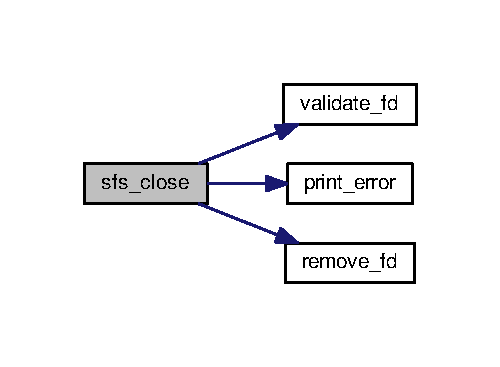
\includegraphics[width=240pt]{close__file_8h_ab89c6dcbc639c5fb3348a6935c12912d_cgraph}
\end{center}
\end{figure}




Here is the caller graph for this function\-:
\nopagebreak
\begin{figure}[H]
\begin{center}
\leavevmode
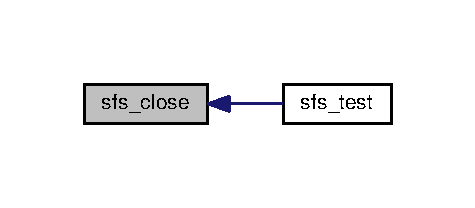
\includegraphics[width=228pt]{close__file_8h_ab89c6dcbc639c5fb3348a6935c12912d_icgraph}
\end{center}
\end{figure}



\hypertarget{create__file_8c}{\section{create\-\_\-file.\-c File Reference}
\label{create__file_8c}\index{create\-\_\-file.\-c@{create\-\_\-file.\-c}}
}
{\ttfamily \#include \char`\"{}glob\-\_\-data.\-h\char`\"{}}\\*
{\ttfamily \#include \char`\"{}super\-\_\-block.\-h\char`\"{}}\\*
{\ttfamily \#include \char`\"{}traverse\-\_\-tree.\-h\char`\"{}}\\*
{\ttfamily \#include \char`\"{}block\-\_\-func.\-h\char`\"{}}\\*
{\ttfamily \#include \char`\"{}create\-\_\-file.\-h\char`\"{}}\\*
{\ttfamily \#include \char`\"{}mount.\-h\char`\"{}}\\*
{\ttfamily \#include $<$string.\-h$>$}\\*
Include dependency graph for create\-\_\-file.\-c\-:
\nopagebreak
\begin{figure}[H]
\begin{center}
\leavevmode
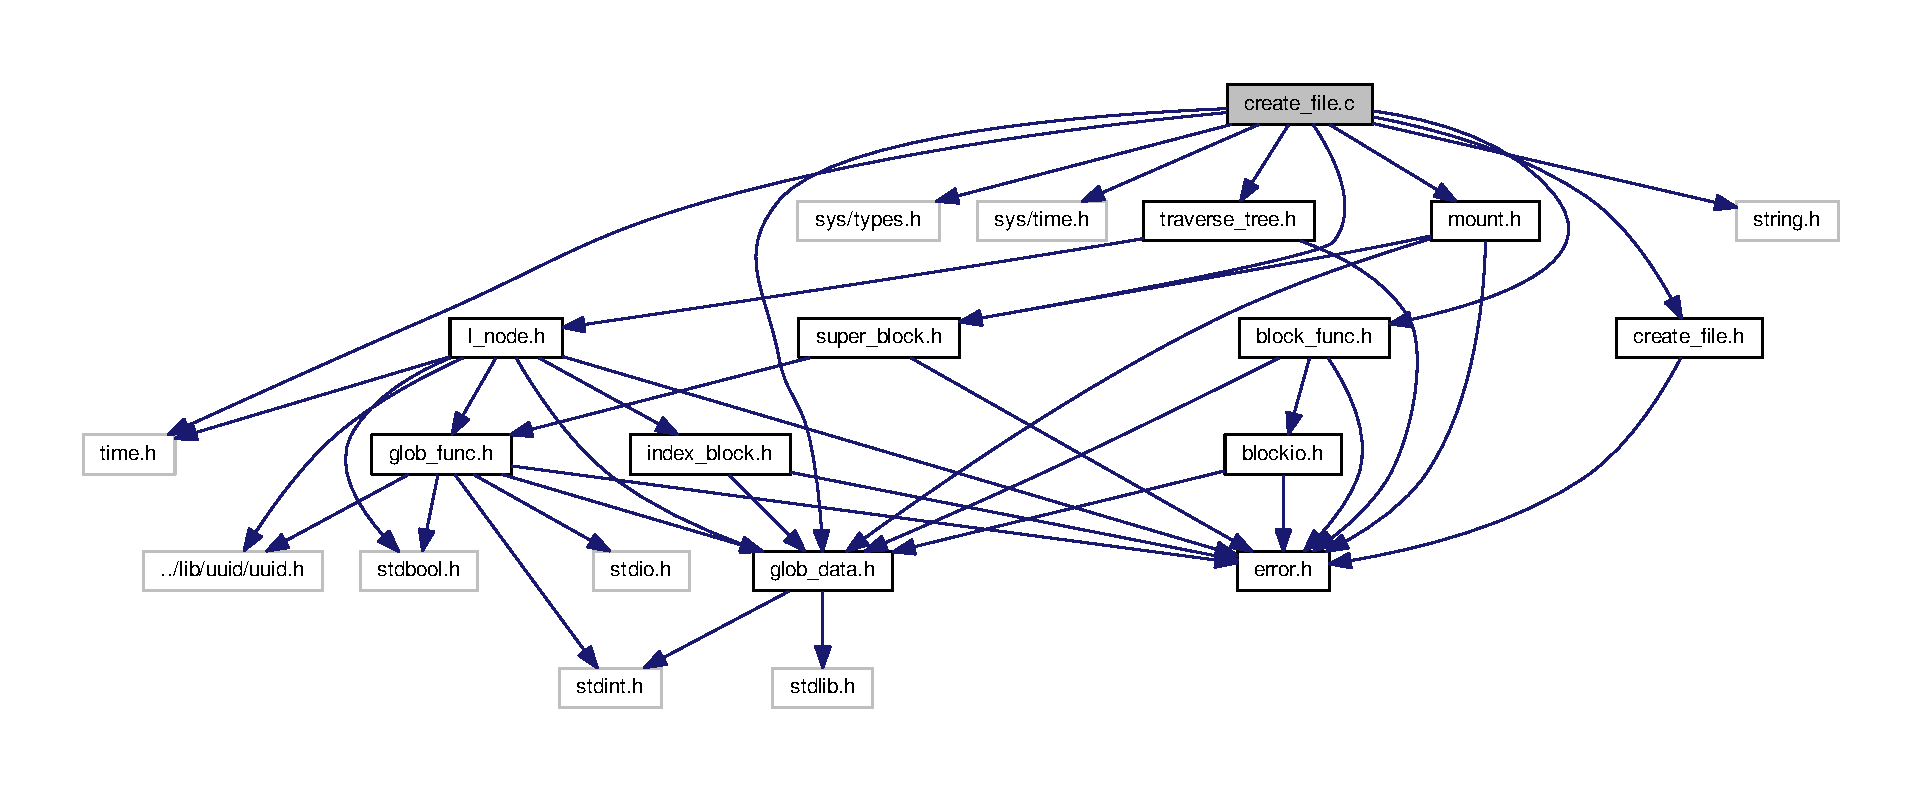
\includegraphics[width=350pt]{create__file_8c__incl}
\end{center}
\end{figure}
\subsection*{Functions}
\begin{DoxyCompactItemize}
\item 
int \hyperlink{create__file_8c_a10498692a07aacf1e88110005e3f2f3f}{sfs\-\_\-create} (char $\ast$pathname, int type)
\begin{DoxyCompactList}\small\item\em Creates a new file or directory at the path specified. \end{DoxyCompactList}\end{DoxyCompactItemize}


\subsection{Function Documentation}
\hypertarget{create__file_8c_a10498692a07aacf1e88110005e3f2f3f}{\index{create\-\_\-file.\-c@{create\-\_\-file.\-c}!sfs\-\_\-create@{sfs\-\_\-create}}
\index{sfs\-\_\-create@{sfs\-\_\-create}!create_file.c@{create\-\_\-file.\-c}}
\subsubsection[{sfs\-\_\-create}]{\setlength{\rightskip}{0pt plus 5cm}int sfs\-\_\-create (
\begin{DoxyParamCaption}
\item[{char $\ast$}]{pathname, }
\item[{int}]{type}
\end{DoxyParamCaption}
)}}\label{create__file_8c_a10498692a07aacf1e88110005e3f2f3f}


Creates a new file or directory at the path specified. 

Create a file with the pathname specified. If there is not already a file with the same pathname, the pathname must contain the full directory path. The parameter type specifies whether a regular file or a directory file should be created.


\begin{DoxyParams}{Parameters}
{\em pathname} & The pathname of file to create, it must be a full directory path.\\
\hline
{\em type} & The type of file to create, zero for a regular file, one for a directory.\\
\hline
\end{DoxyParams}
\begin{DoxyReturn}{Returns}
Returns an integer value. If the value $>$ 0 the file creation was a success, and if the value $<$= 0 the file createion was unsuccessful.
\end{DoxyReturn}

\begin{DoxyExceptions}{Exceptions}
{\em I\-N\-V\-A\-L\-I\-D\-\_\-\-F\-I\-L\-E\-\_\-\-N\-A\-M\-E} & If the specified file name is already in use.\\
\hline
{\em I\-N\-V\-A\-L\-I\-D\-\_\-\-F\-I\-L\-E\-\_\-\-T\-Y\-P\-E} & If the file type specified is not a regular file (0) or a directory file (1).\\
\hline
{\em I\-N\-V\-A\-L\-I\-D\-\_\-\-P\-A\-T\-H} & If the pathname specified does not already exist.\\
\hline
{\em I\-N\-S\-U\-F\-F\-I\-C\-I\-E\-N\-T\-\_\-\-D\-I\-S\-K\-\_\-\-S\-P\-A\-C\-E} & If the length of the blocks to be written is greater than the amount of available blocks on disk.\\
\hline
\end{DoxyExceptions}
\begin{DoxyAuthor}{Author}
Daniel Smullen

Jonathan Gillett

Joseph Heron
\end{DoxyAuthor}
\begin{DoxyCopyright}{Copyright}
G\-N\-U General Public License V3 
\end{DoxyCopyright}


Here is the call graph for this function\-:
\nopagebreak
\begin{figure}[H]
\begin{center}
\leavevmode
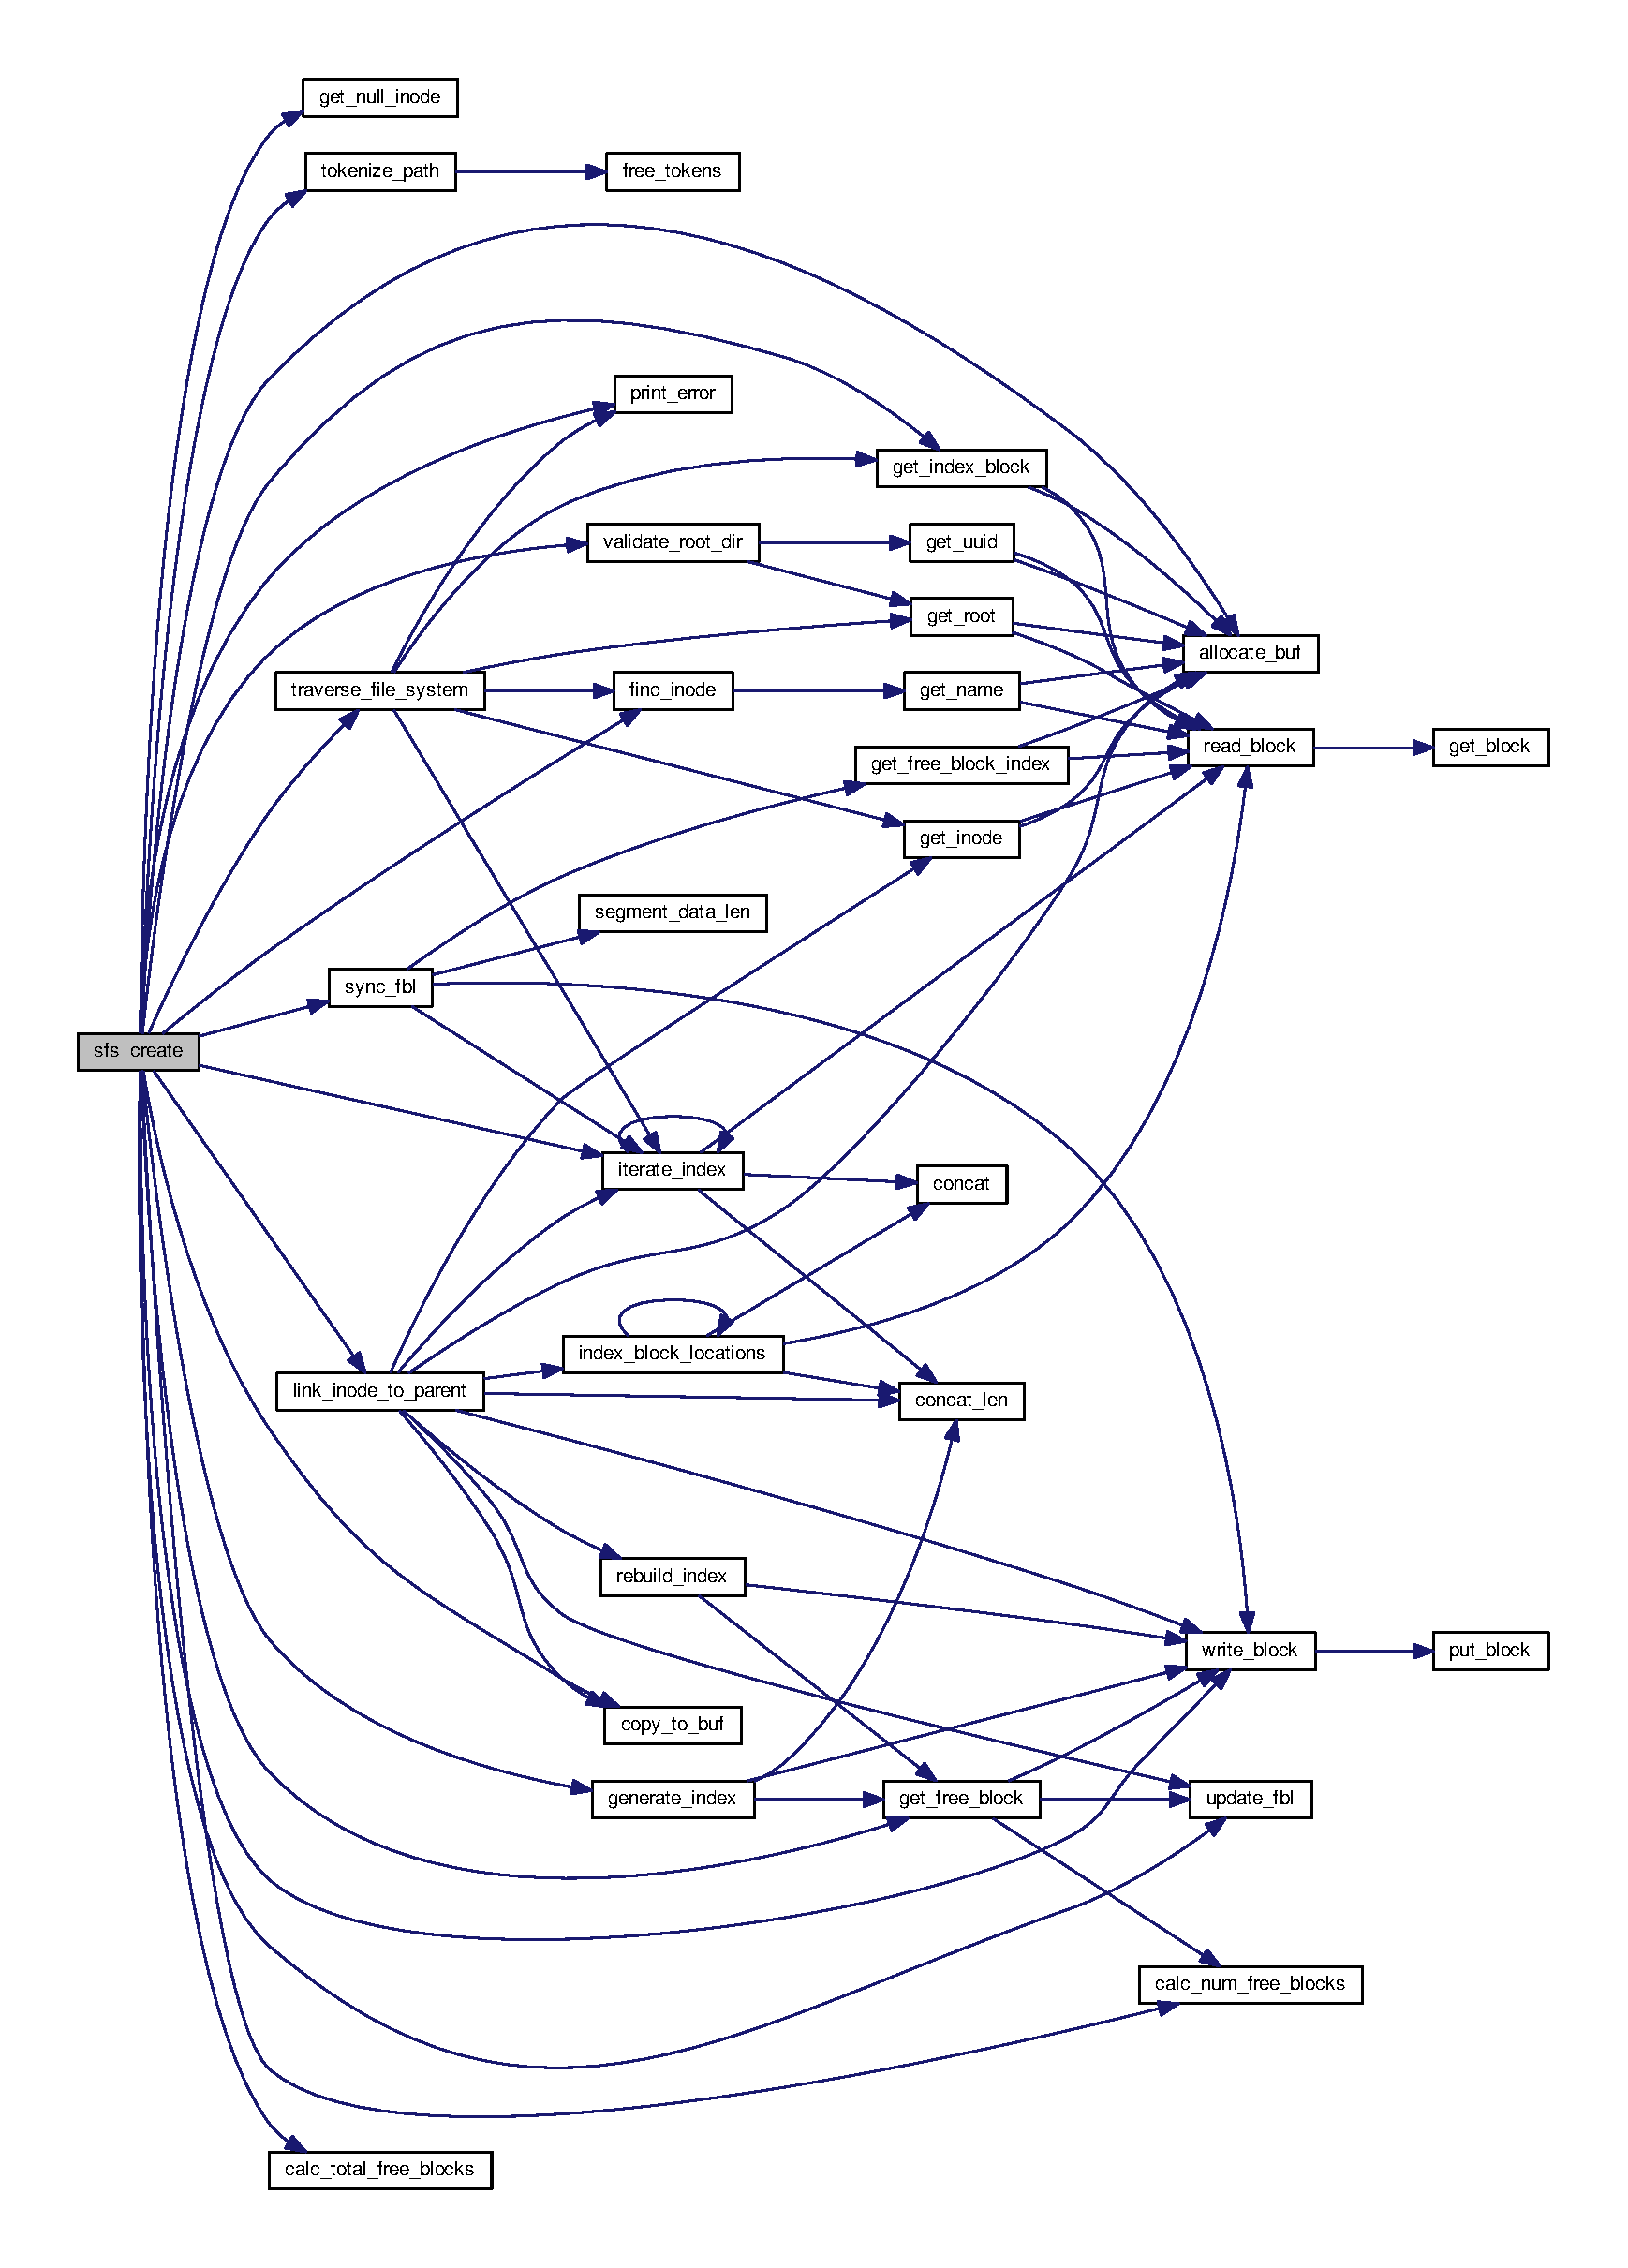
\includegraphics[width=350pt]{create__file_8c_a10498692a07aacf1e88110005e3f2f3f_cgraph}
\end{center}
\end{figure}




Here is the caller graph for this function\-:
\nopagebreak
\begin{figure}[H]
\begin{center}
\leavevmode
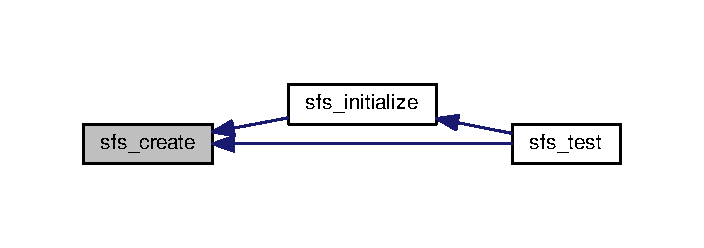
\includegraphics[width=338pt]{create__file_8c_a10498692a07aacf1e88110005e3f2f3f_icgraph}
\end{center}
\end{figure}



\hypertarget{create__file_8h}{\section{create\-\_\-file.\-h File Reference}
\label{create__file_8h}\index{create\-\_\-file.\-h@{create\-\_\-file.\-h}}
}
{\ttfamily \#include \char`\"{}error.\-h\char`\"{}}\\*
Include dependency graph for create\-\_\-file.\-h\-:
\nopagebreak
\begin{figure}[H]
\begin{center}
\leavevmode
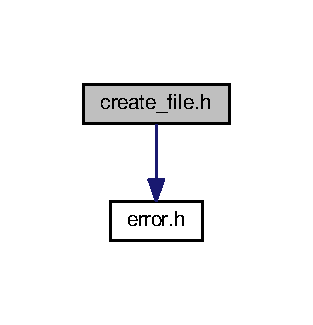
\includegraphics[width=150pt]{create__file_8h__incl}
\end{center}
\end{figure}
This graph shows which files directly or indirectly include this file\-:
\nopagebreak
\begin{figure}[H]
\begin{center}
\leavevmode
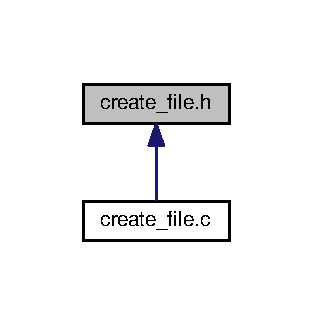
\includegraphics[width=150pt]{create__file_8h__dep__incl}
\end{center}
\end{figure}
\subsection*{Macros}
\begin{DoxyCompactItemize}
\item 
\#define \hyperlink{create__file_8h_a24b6ce12efa0d5ace6b2869080b3ea12}{C\-R\-E\-A\-T\-E\-\_\-\-S\-I\-Z\-E}~2
\end{DoxyCompactItemize}
\subsection*{Functions}
\begin{DoxyCompactItemize}
\item 
int \hyperlink{create__file_8h_a10498692a07aacf1e88110005e3f2f3f}{sfs\-\_\-create} (char $\ast$pathname, int type)
\begin{DoxyCompactList}\small\item\em Creates a new file or directory at the path specified. \end{DoxyCompactList}\end{DoxyCompactItemize}


\subsection{Macro Definition Documentation}
\hypertarget{create__file_8h_a24b6ce12efa0d5ace6b2869080b3ea12}{\index{create\-\_\-file.\-h@{create\-\_\-file.\-h}!C\-R\-E\-A\-T\-E\-\_\-\-S\-I\-Z\-E@{C\-R\-E\-A\-T\-E\-\_\-\-S\-I\-Z\-E}}
\index{C\-R\-E\-A\-T\-E\-\_\-\-S\-I\-Z\-E@{C\-R\-E\-A\-T\-E\-\_\-\-S\-I\-Z\-E}!create_file.h@{create\-\_\-file.\-h}}
\subsubsection[{C\-R\-E\-A\-T\-E\-\_\-\-S\-I\-Z\-E}]{\setlength{\rightskip}{0pt plus 5cm}\#define C\-R\-E\-A\-T\-E\-\_\-\-S\-I\-Z\-E~2}}\label{create__file_8h_a24b6ce12efa0d5ace6b2869080b3ea12}


\subsection{Function Documentation}
\hypertarget{create__file_8h_a10498692a07aacf1e88110005e3f2f3f}{\index{create\-\_\-file.\-h@{create\-\_\-file.\-h}!sfs\-\_\-create@{sfs\-\_\-create}}
\index{sfs\-\_\-create@{sfs\-\_\-create}!create_file.h@{create\-\_\-file.\-h}}
\subsubsection[{sfs\-\_\-create}]{\setlength{\rightskip}{0pt plus 5cm}int sfs\-\_\-create (
\begin{DoxyParamCaption}
\item[{char $\ast$}]{pathname, }
\item[{int}]{type}
\end{DoxyParamCaption}
)}}\label{create__file_8h_a10498692a07aacf1e88110005e3f2f3f}


Creates a new file or directory at the path specified. 

Create a file with the pathname specified. If there is not already a file with the same pathname, the pathname must contain the full directory path. The parameter type specifies whether a regular file or a directory file should be created.


\begin{DoxyParams}{Parameters}
{\em pathname} & The pathname of file to create, it must be a full directory path.\\
\hline
{\em type} & The type of file to create, zero for a regular file, one for a directory.\\
\hline
\end{DoxyParams}
\begin{DoxyReturn}{Returns}
Returns an integer value. If the value $>$ 0 the file creation was a success, and if the value $<$= 0 the file createion was unsuccessful.
\end{DoxyReturn}

\begin{DoxyExceptions}{Exceptions}
{\em I\-N\-V\-A\-L\-I\-D\-\_\-\-F\-I\-L\-E\-\_\-\-N\-A\-M\-E} & If the specified file name is already in use.\\
\hline
{\em I\-N\-V\-A\-L\-I\-D\-\_\-\-F\-I\-L\-E\-\_\-\-T\-Y\-P\-E} & If the file type specified is not a regular file (0) or a directory file (1).\\
\hline
{\em I\-N\-V\-A\-L\-I\-D\-\_\-\-P\-A\-T\-H} & If the pathname specified does not already exist.\\
\hline
{\em I\-N\-S\-U\-F\-F\-I\-C\-I\-E\-N\-T\-\_\-\-D\-I\-S\-K\-\_\-\-S\-P\-A\-C\-E} & If the length of the blocks to be written is greater than the amount of available blocks on disk.\\
\hline
\end{DoxyExceptions}
\begin{DoxyAuthor}{Author}
Daniel Smullen

Jonathan Gillett

Joseph Heron
\end{DoxyAuthor}
\begin{DoxyCopyright}{Copyright}
G\-N\-U General Public License V3 
\end{DoxyCopyright}


Here is the call graph for this function\-:
\nopagebreak
\begin{figure}[H]
\begin{center}
\leavevmode
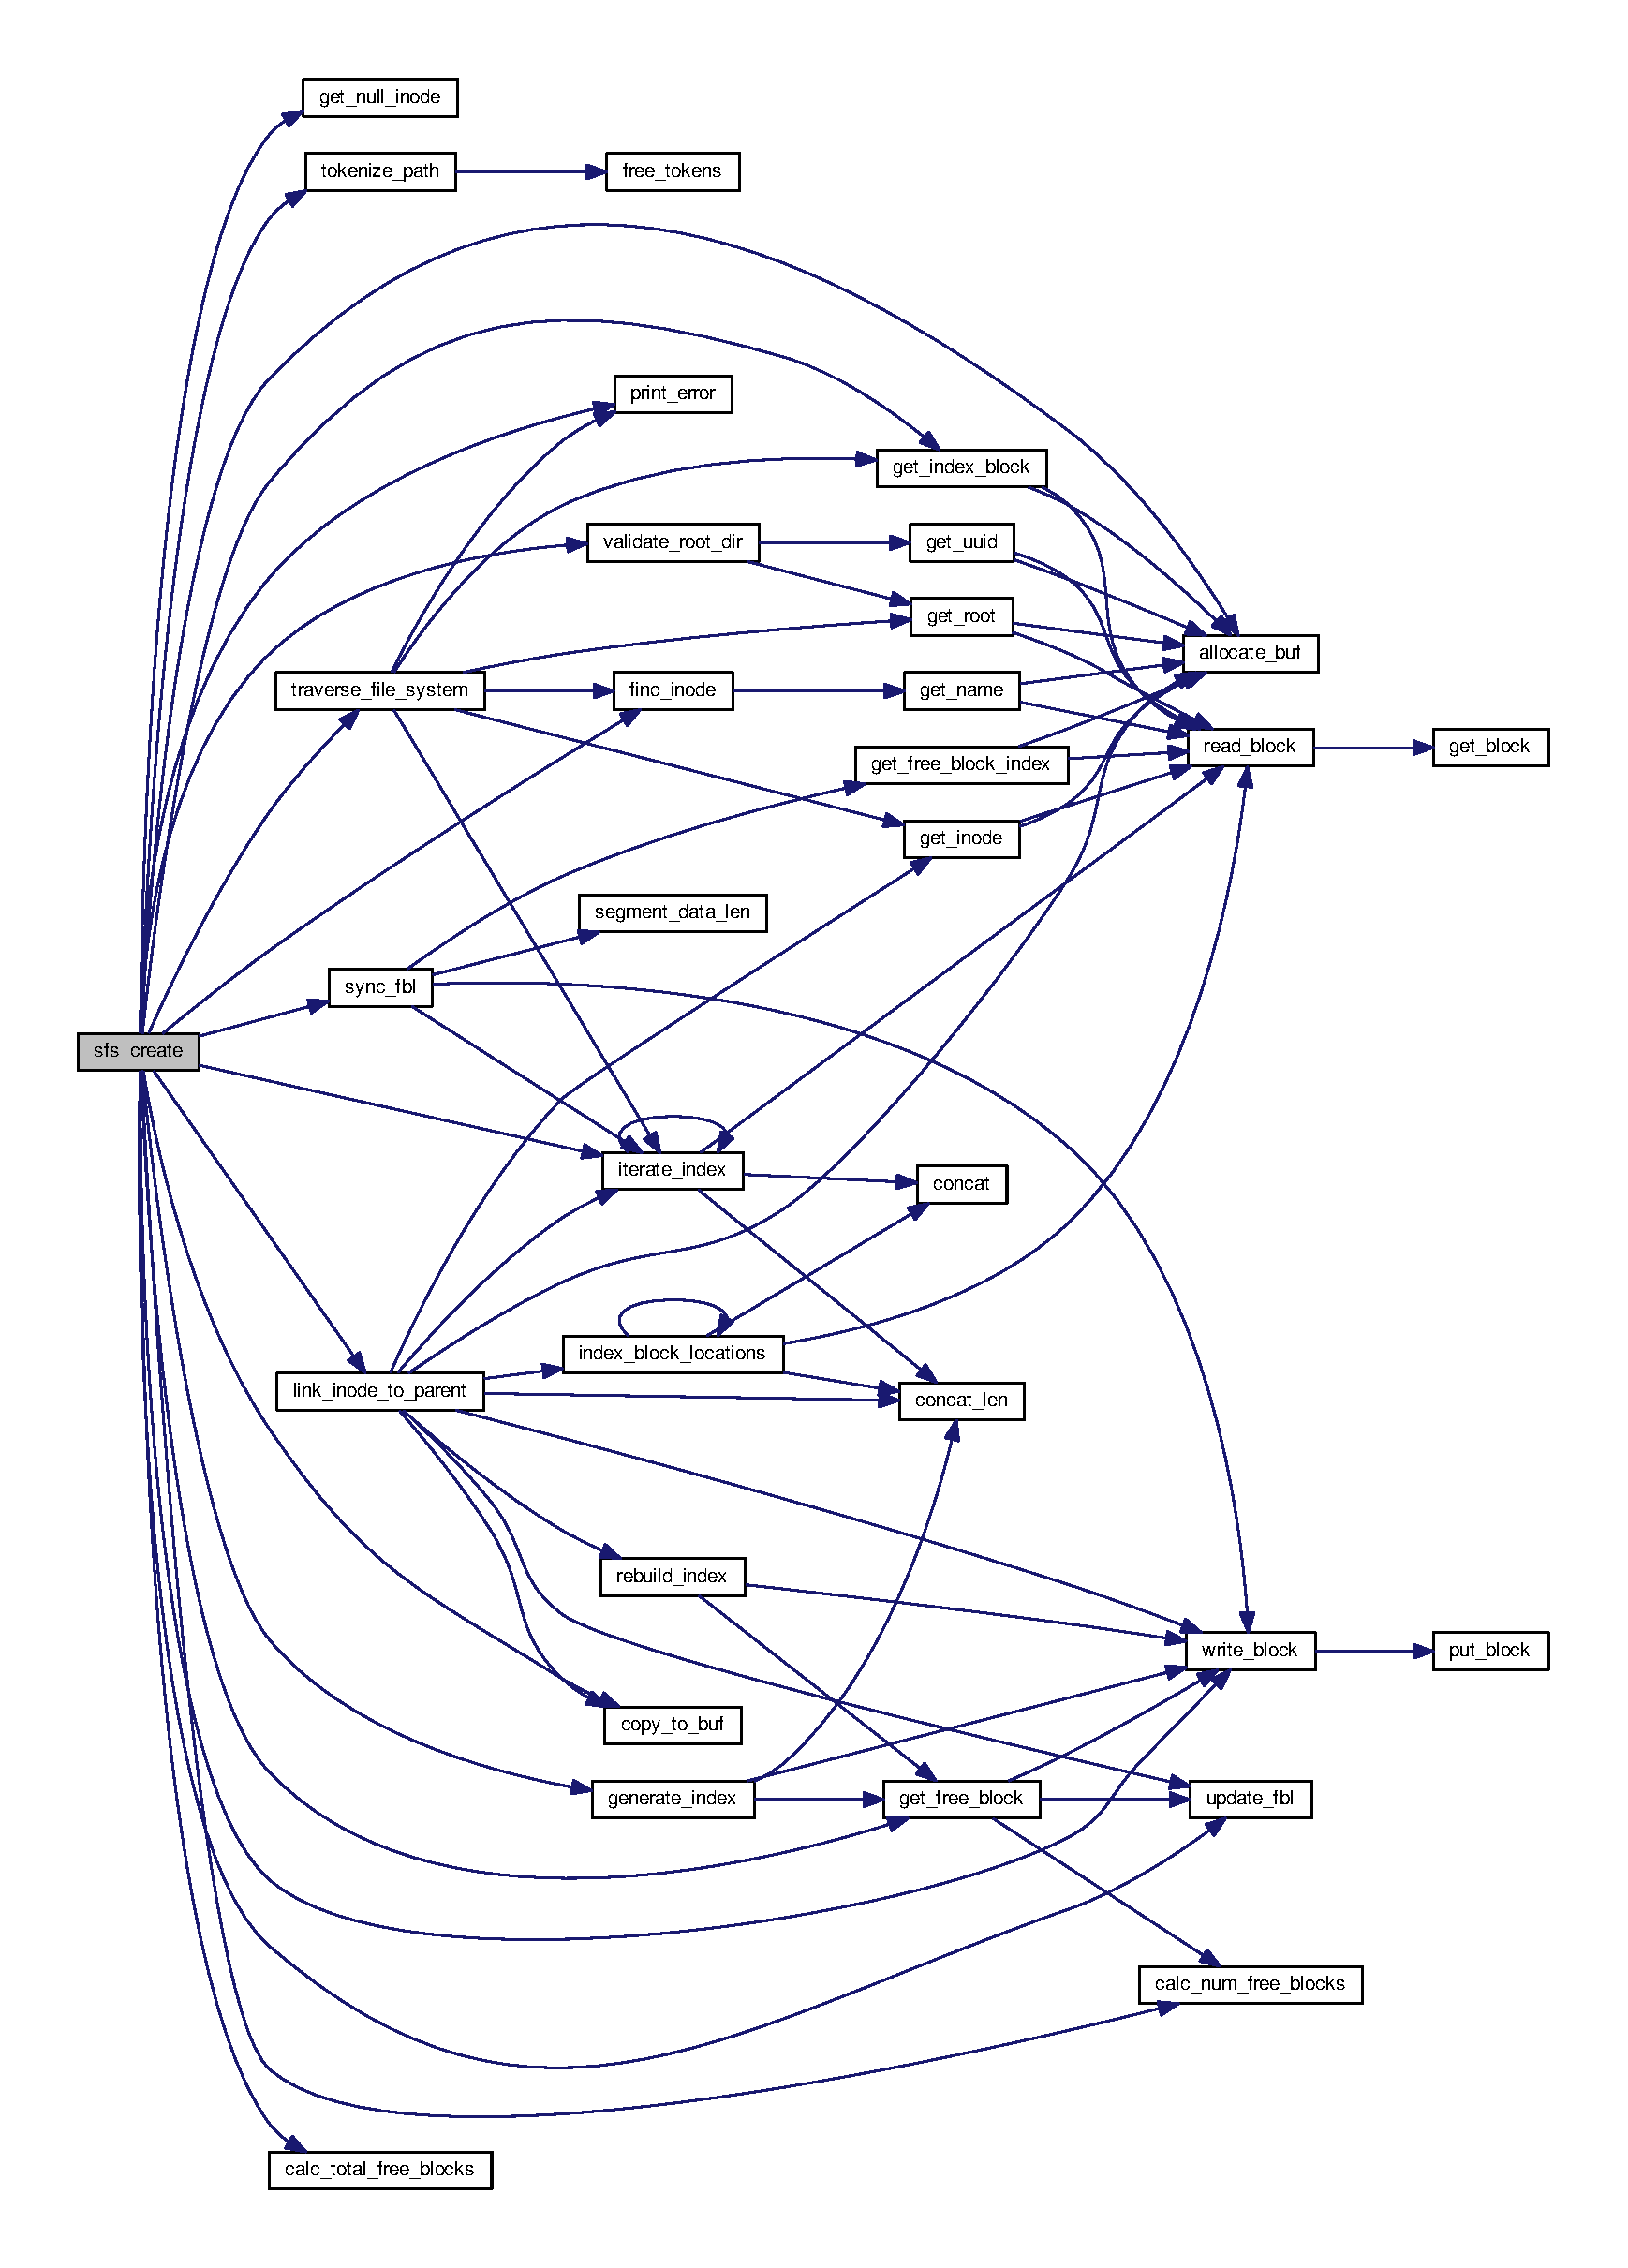
\includegraphics[width=350pt]{create__file_8h_a10498692a07aacf1e88110005e3f2f3f_cgraph}
\end{center}
\end{figure}




Here is the caller graph for this function\-:
\nopagebreak
\begin{figure}[H]
\begin{center}
\leavevmode
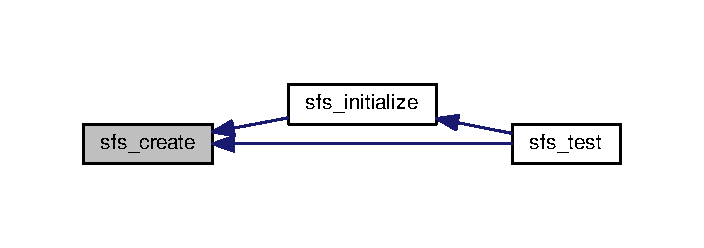
\includegraphics[width=338pt]{create__file_8h_a10498692a07aacf1e88110005e3f2f3f_icgraph}
\end{center}
\end{figure}



\hypertarget{delete__file_8c}{\section{delete\-\_\-file.\-c File Reference}
\label{delete__file_8c}\index{delete\-\_\-file.\-c@{delete\-\_\-file.\-c}}
}
{\ttfamily \#include \char`\"{}glob\-\_\-data.\-h\char`\"{}}\\*
{\ttfamily \#include \char`\"{}blockio.\-h\char`\"{}}\\*
{\ttfamily \#include \char`\"{}traverse\-\_\-tree.\-h\char`\"{}}\\*
{\ttfamily \#include \char`\"{}free\-\_\-block\-\_\-list.\-h\char`\"{}}\\*
{\ttfamily \#include \char`\"{}system\-\_\-open\-\_\-file\-\_\-table.\-h\char`\"{}}\\*
{\ttfamily \#include \char`\"{}delete\-\_\-file.\-h\char`\"{}}\\*
Include dependency graph for delete\-\_\-file.\-c\-:
\nopagebreak
\begin{figure}[H]
\begin{center}
\leavevmode
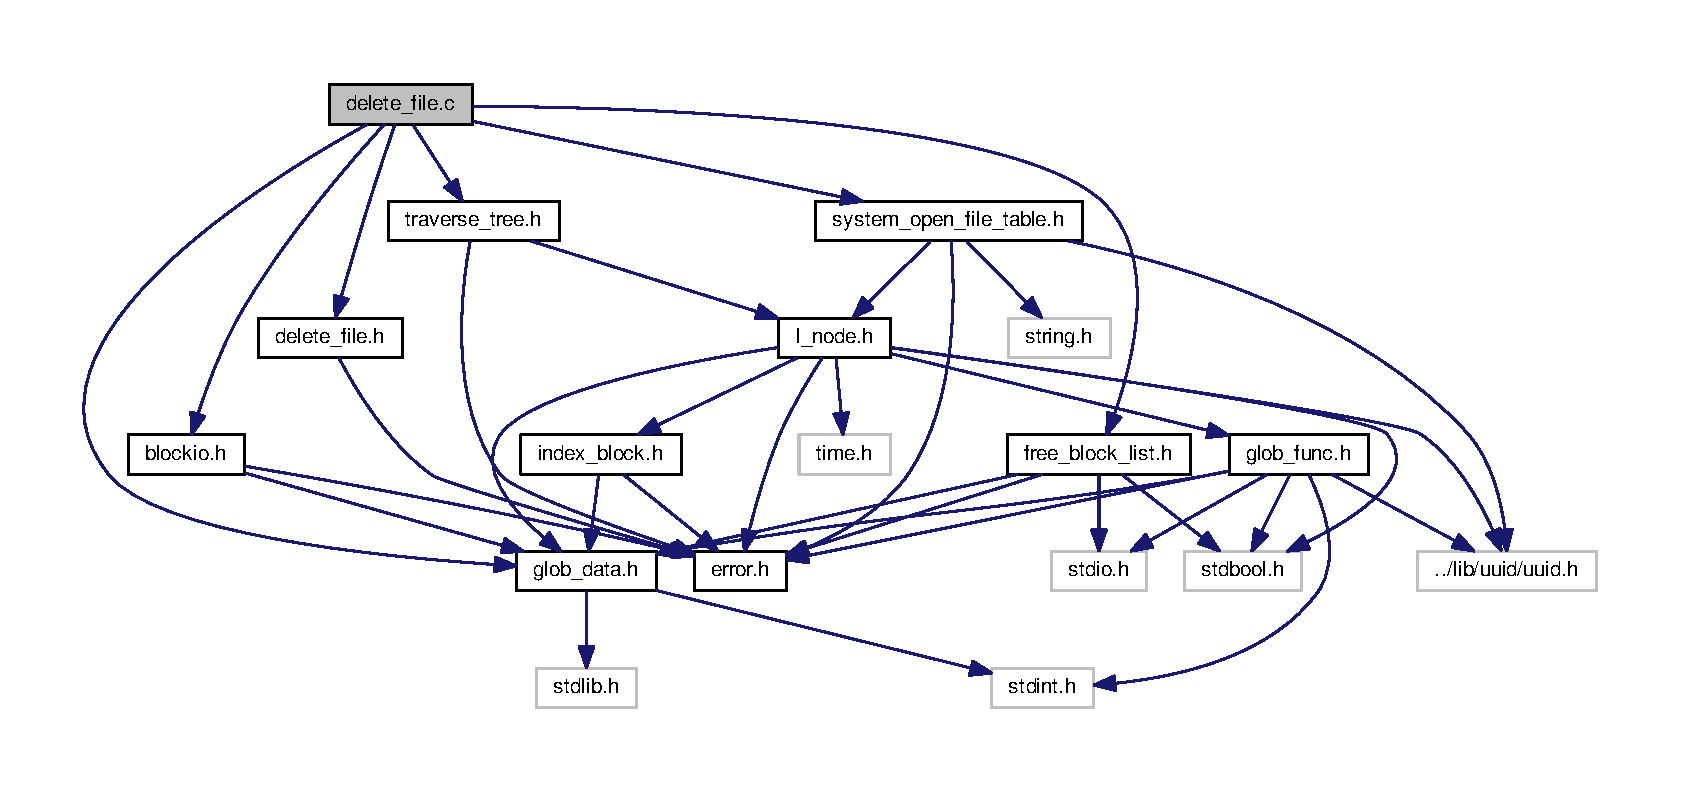
\includegraphics[width=350pt]{delete__file_8c__incl}
\end{center}
\end{figure}
\subsection*{Functions}
\begin{DoxyCompactItemize}
\item 
int \hyperlink{delete__file_8c_ad7cc263f6e467c2eb2f8f73a6eb9d1c3}{sfs\-\_\-delete} (char $\ast$pathname)
\begin{DoxyCompactList}\small\item\em Delete a file with the pathname specified. \end{DoxyCompactList}\end{DoxyCompactItemize}


\subsection{Function Documentation}
\hypertarget{delete__file_8c_ad7cc263f6e467c2eb2f8f73a6eb9d1c3}{\index{delete\-\_\-file.\-c@{delete\-\_\-file.\-c}!sfs\-\_\-delete@{sfs\-\_\-delete}}
\index{sfs\-\_\-delete@{sfs\-\_\-delete}!delete_file.c@{delete\-\_\-file.\-c}}
\subsubsection[{sfs\-\_\-delete}]{\setlength{\rightskip}{0pt plus 5cm}int sfs\-\_\-delete (
\begin{DoxyParamCaption}
\item[{char $\ast$}]{pathname}
\end{DoxyParamCaption}
)}}\label{delete__file_8c_ad7cc263f6e467c2eb2f8f73a6eb9d1c3}


Delete a file with the pathname specified. 


\begin{DoxyParams}{Parameters}
{\em pathname} & The pathname of file to create, must be full directory path\\
\hline
\end{DoxyParams}
\begin{DoxyReturn}{Returns}
Returns an integer value, if the value is $>$ 0 then the file was deleted successfully. If the value is $<$= 0 then the file failed to delete.
\end{DoxyReturn}

\begin{DoxyExceptions}{Exceptions}
{\em F\-I\-L\-E\-\_\-\-N\-O\-T\-\_\-\-F\-O\-U\-N\-D} & If the file at the specified path does not already exist.\\
\hline
\end{DoxyExceptions}
\begin{DoxyAuthor}{Author}
Daniel Smullen

Jonathan Gillett

Joseph Heron
\end{DoxyAuthor}
\begin{DoxyCopyright}{Copyright}
G\-N\-U General Public License V3 
\end{DoxyCopyright}


Here is the call graph for this function\-:
\nopagebreak
\begin{figure}[H]
\begin{center}
\leavevmode
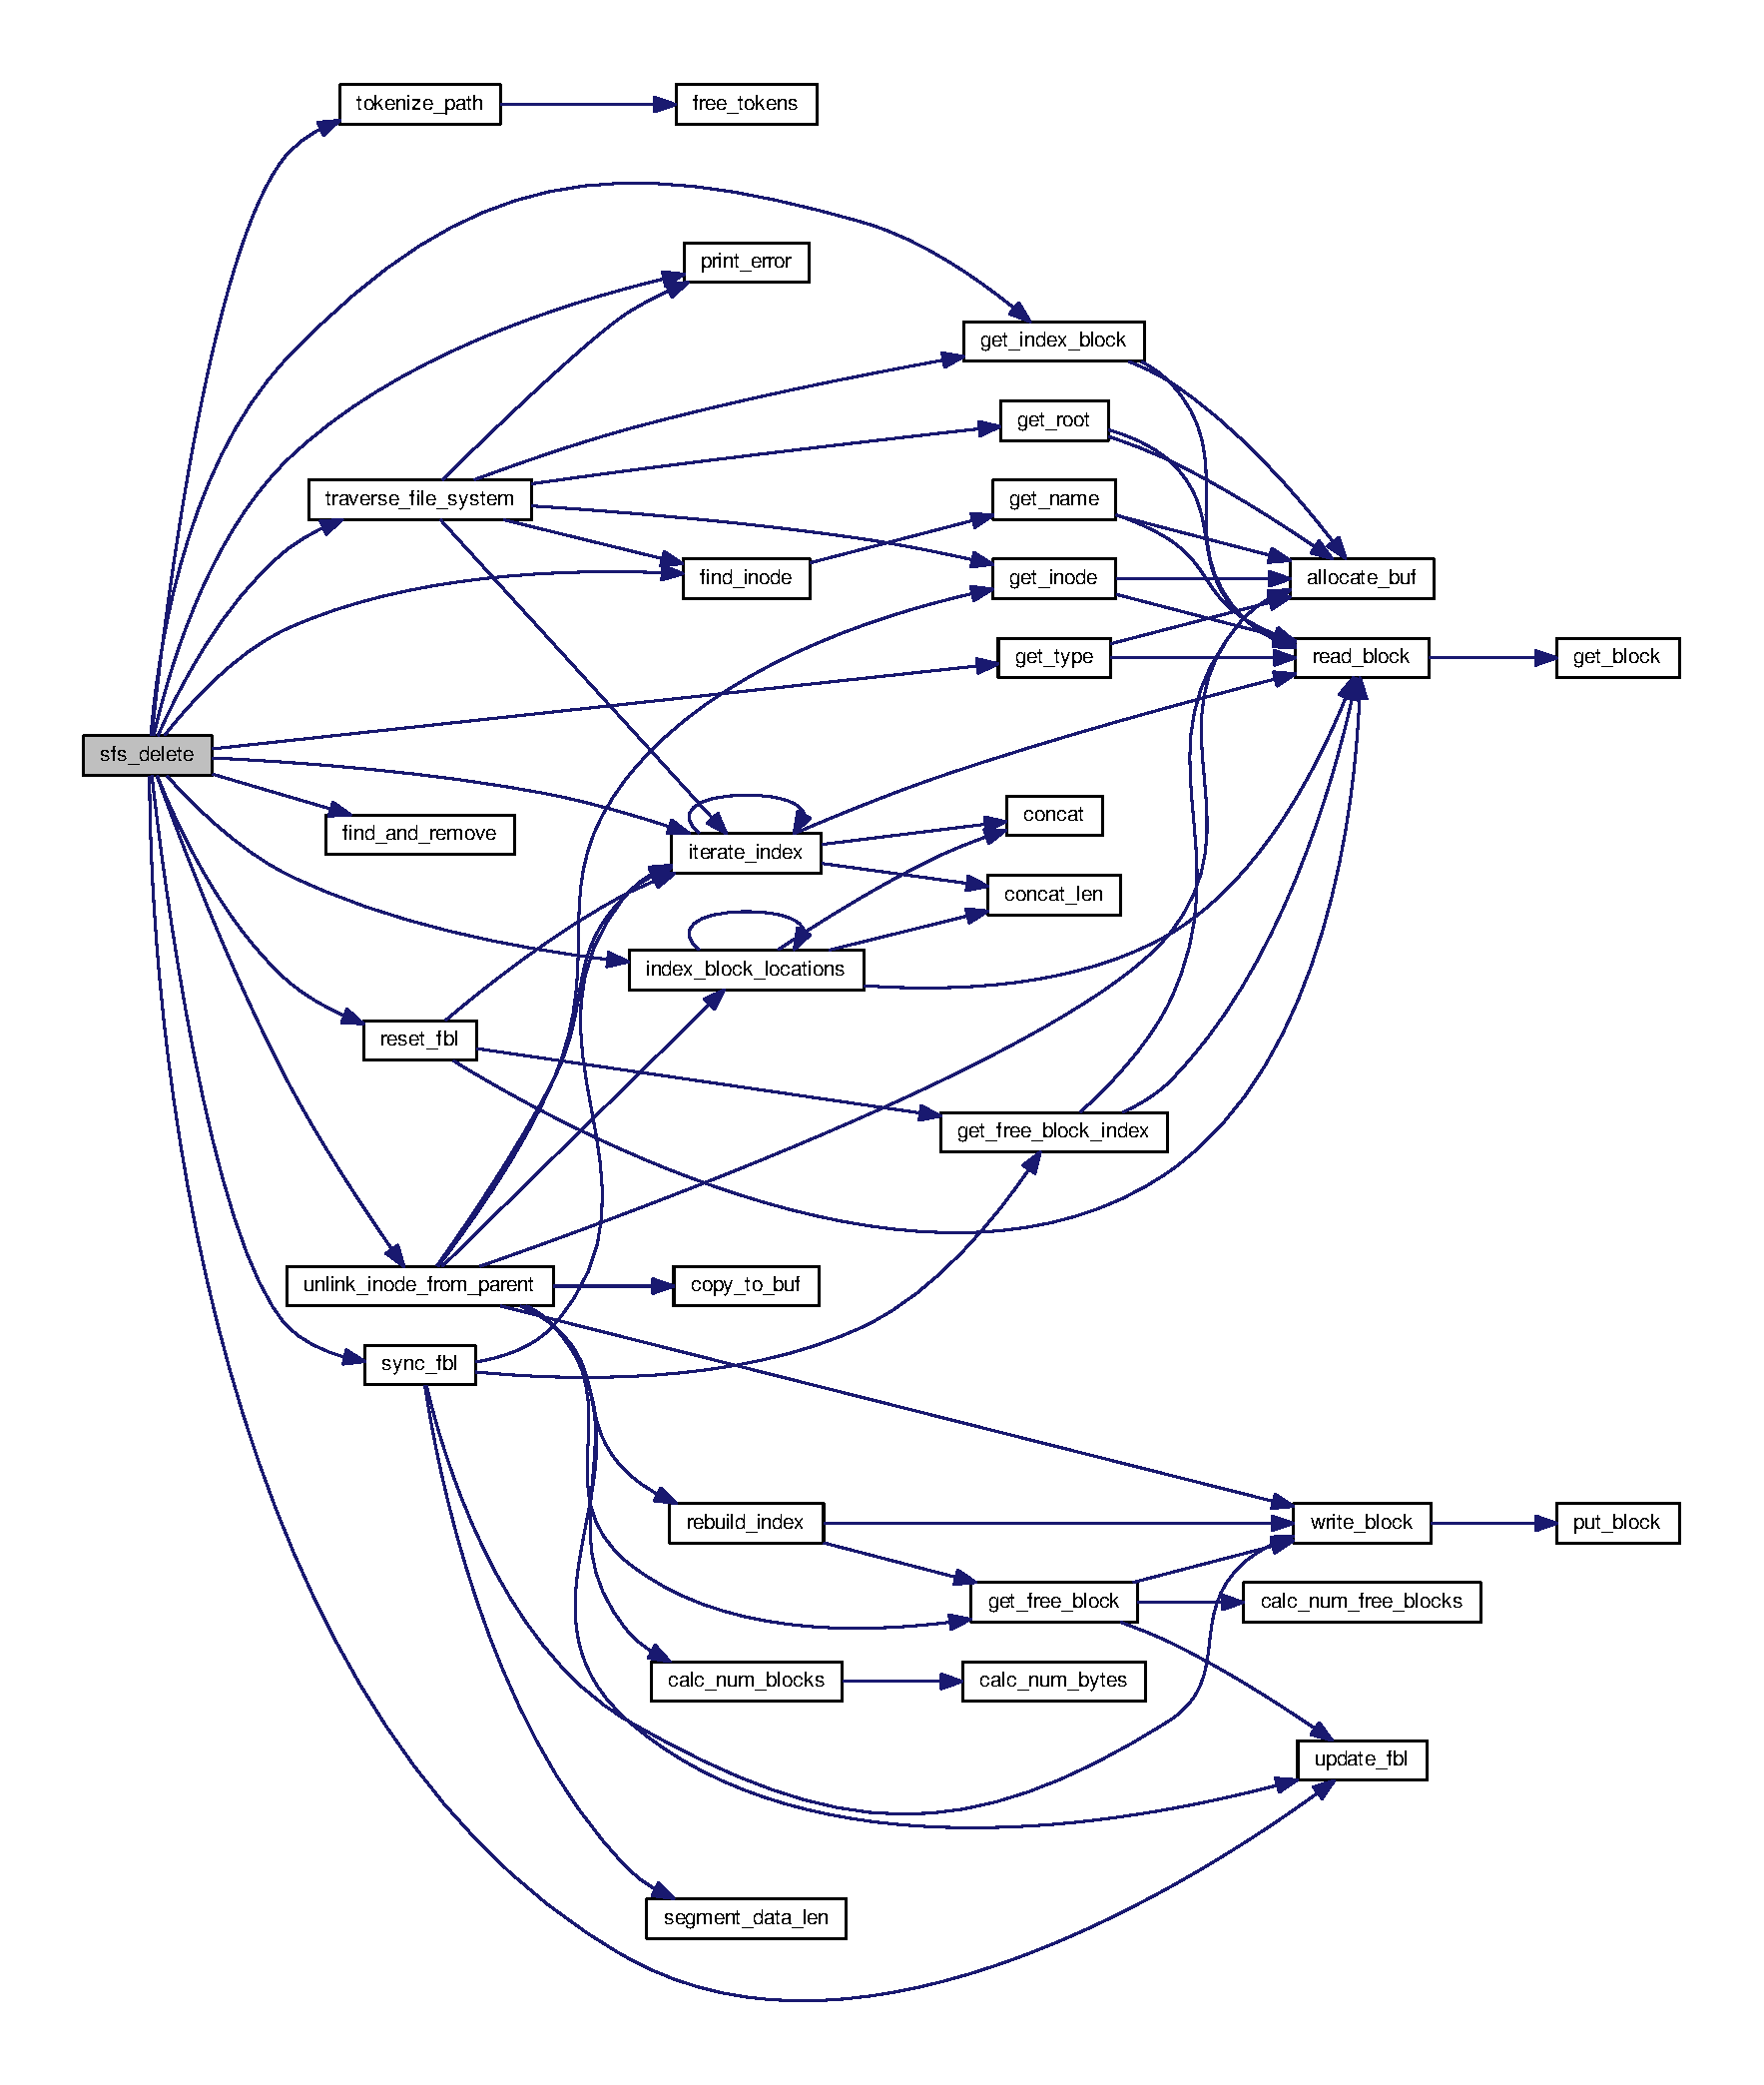
\includegraphics[width=350pt]{delete__file_8c_ad7cc263f6e467c2eb2f8f73a6eb9d1c3_cgraph}
\end{center}
\end{figure}




Here is the caller graph for this function\-:
\nopagebreak
\begin{figure}[H]
\begin{center}
\leavevmode
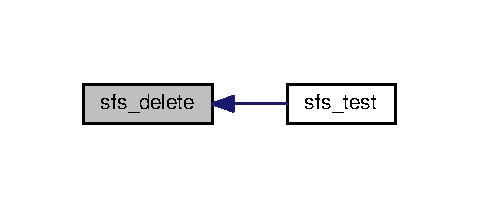
\includegraphics[width=230pt]{delete__file_8c_ad7cc263f6e467c2eb2f8f73a6eb9d1c3_icgraph}
\end{center}
\end{figure}



\hypertarget{delete__file_8h}{\section{delete\-\_\-file.\-h File Reference}
\label{delete__file_8h}\index{delete\-\_\-file.\-h@{delete\-\_\-file.\-h}}
}
{\ttfamily \#include \char`\"{}error.\-h\char`\"{}}\\*
Include dependency graph for delete\-\_\-file.\-h\-:
\nopagebreak
\begin{figure}[H]
\begin{center}
\leavevmode
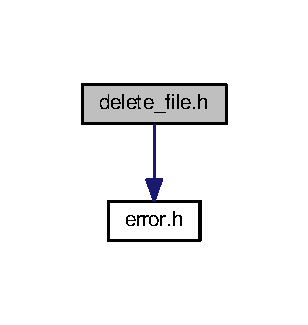
\includegraphics[width=148pt]{delete__file_8h__incl}
\end{center}
\end{figure}
This graph shows which files directly or indirectly include this file\-:
\nopagebreak
\begin{figure}[H]
\begin{center}
\leavevmode
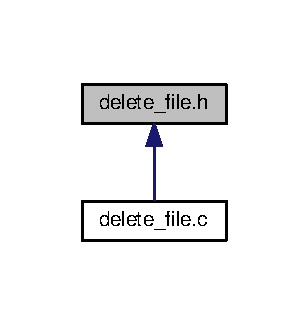
\includegraphics[width=148pt]{delete__file_8h__dep__incl}
\end{center}
\end{figure}
\subsection*{Functions}
\begin{DoxyCompactItemize}
\item 
int \hyperlink{delete__file_8h_ad7cc263f6e467c2eb2f8f73a6eb9d1c3}{sfs\-\_\-delete} (char $\ast$pathname)
\begin{DoxyCompactList}\small\item\em Delete a file with the pathname specified. \end{DoxyCompactList}\end{DoxyCompactItemize}


\subsection{Function Documentation}
\hypertarget{delete__file_8h_ad7cc263f6e467c2eb2f8f73a6eb9d1c3}{\index{delete\-\_\-file.\-h@{delete\-\_\-file.\-h}!sfs\-\_\-delete@{sfs\-\_\-delete}}
\index{sfs\-\_\-delete@{sfs\-\_\-delete}!delete_file.h@{delete\-\_\-file.\-h}}
\subsubsection[{sfs\-\_\-delete}]{\setlength{\rightskip}{0pt plus 5cm}int sfs\-\_\-delete (
\begin{DoxyParamCaption}
\item[{char $\ast$}]{pathname}
\end{DoxyParamCaption}
)}}\label{delete__file_8h_ad7cc263f6e467c2eb2f8f73a6eb9d1c3}


Delete a file with the pathname specified. 


\begin{DoxyParams}{Parameters}
{\em pathname} & The pathname of file to create, must be full directory path\\
\hline
\end{DoxyParams}
\begin{DoxyReturn}{Returns}
Returns an integer value, if the value is $>$ 0 then the file was deleted successfully. If the value is $<$= 0 then the file failed to delete.
\end{DoxyReturn}

\begin{DoxyExceptions}{Exceptions}
{\em F\-I\-L\-E\-\_\-\-N\-O\-T\-\_\-\-F\-O\-U\-N\-D} & If the file at the specified path does not already exist.\\
\hline
\end{DoxyExceptions}
\begin{DoxyAuthor}{Author}
Daniel Smullen

Jonathan Gillett

Joseph Heron
\end{DoxyAuthor}
\begin{DoxyCopyright}{Copyright}
G\-N\-U General Public License V3 
\end{DoxyCopyright}


Here is the call graph for this function\-:
\nopagebreak
\begin{figure}[H]
\begin{center}
\leavevmode
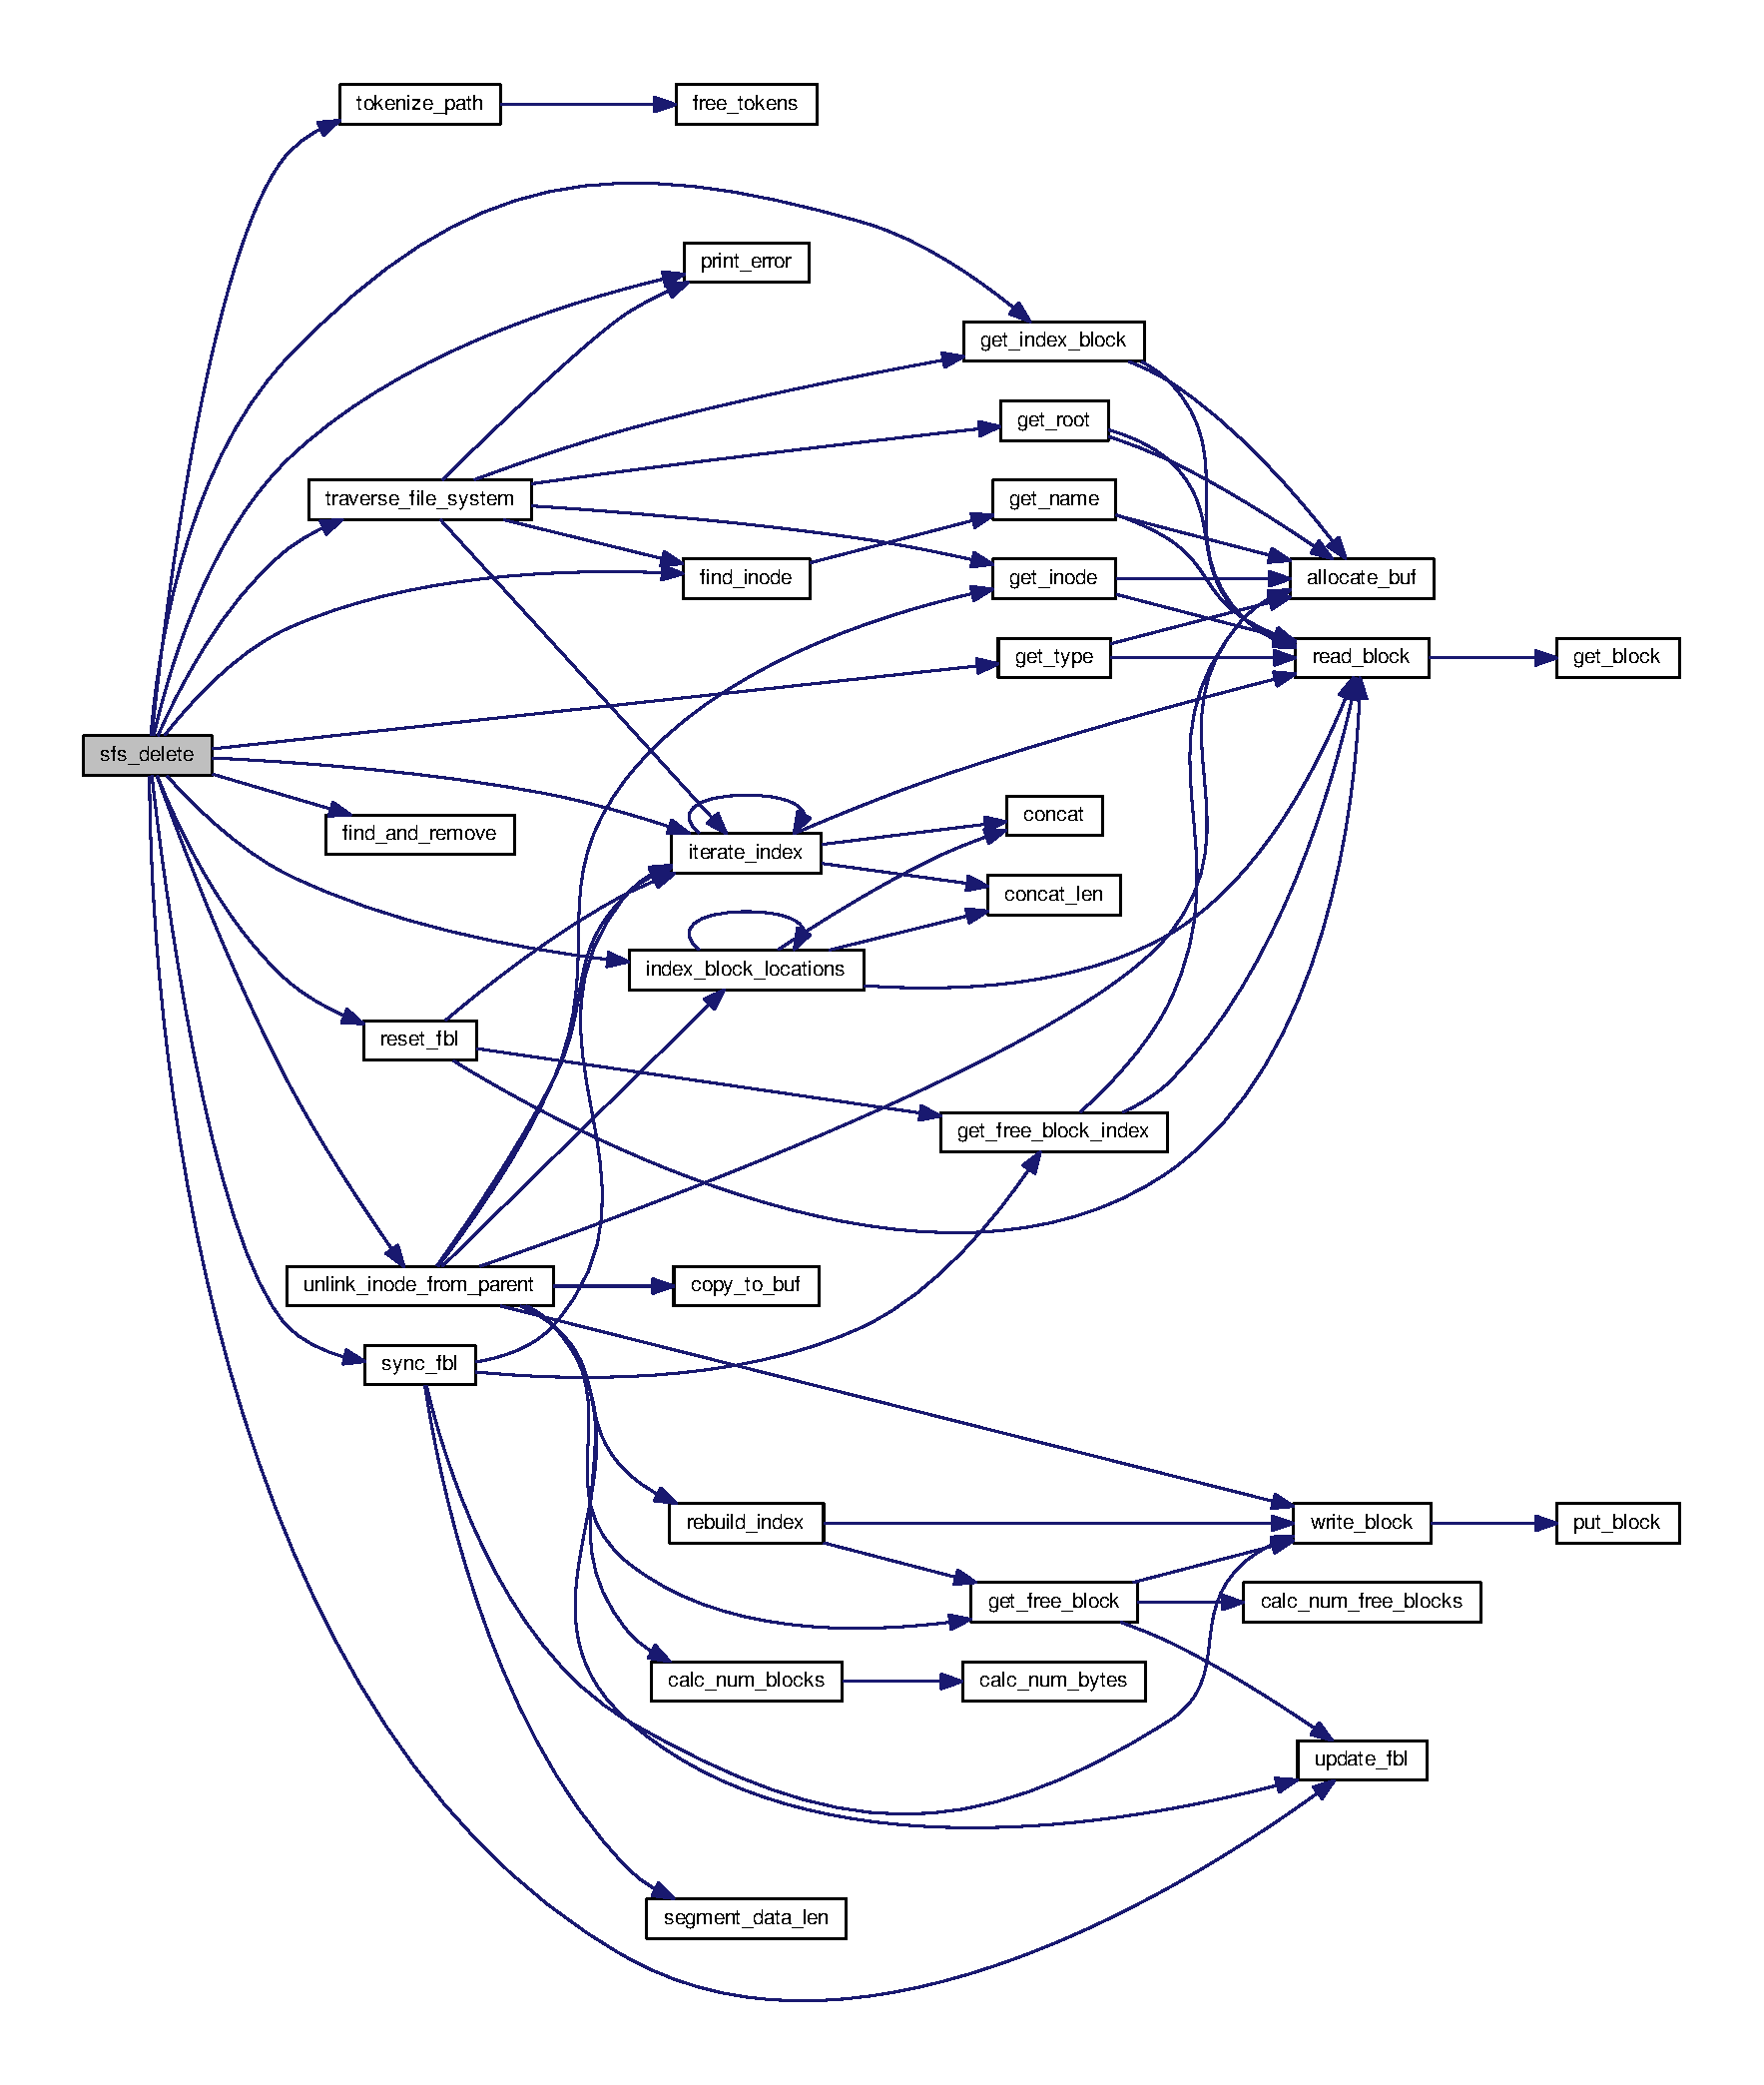
\includegraphics[width=350pt]{delete__file_8h_ad7cc263f6e467c2eb2f8f73a6eb9d1c3_cgraph}
\end{center}
\end{figure}




Here is the caller graph for this function\-:
\nopagebreak
\begin{figure}[H]
\begin{center}
\leavevmode
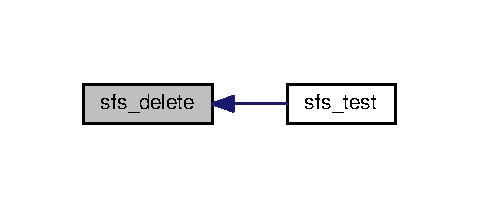
\includegraphics[width=230pt]{delete__file_8h_ad7cc263f6e467c2eb2f8f73a6eb9d1c3_icgraph}
\end{center}
\end{figure}



\hypertarget{error_8c}{\section{error.\-c File Reference}
\label{error_8c}\index{error.\-c@{error.\-c}}
}
{\ttfamily \#include \char`\"{}error.\-h\char`\"{}}\\*
Include dependency graph for error.\-c\-:
\nopagebreak
\begin{figure}[H]
\begin{center}
\leavevmode
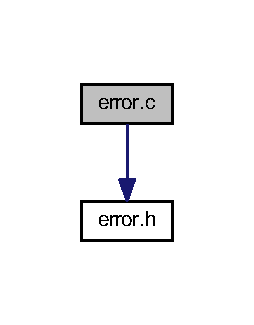
\includegraphics[width=122pt]{error_8c__incl}
\end{center}
\end{figure}
\subsection*{Functions}
\begin{DoxyCompactItemize}
\item 
void \hyperlink{error_8c_af85f0519da49c9e50bf3d1feffa74ef3}{print\-\_\-error} (\hyperlink{error_8h_a88a76ee847c844cc47b94caac600689d}{error\-\_\-code} errorno)
\begin{DoxyCompactList}\small\item\em Prints an error code. \end{DoxyCompactList}\end{DoxyCompactItemize}


\subsection{Function Documentation}
\hypertarget{error_8c_af85f0519da49c9e50bf3d1feffa74ef3}{\index{error.\-c@{error.\-c}!print\-\_\-error@{print\-\_\-error}}
\index{print\-\_\-error@{print\-\_\-error}!error.c@{error.\-c}}
\subsubsection[{print\-\_\-error}]{\setlength{\rightskip}{0pt plus 5cm}void print\-\_\-error (
\begin{DoxyParamCaption}
\item[{{\bf error\-\_\-code}}]{errorno}
\end{DoxyParamCaption}
)}}\label{error_8c_af85f0519da49c9e50bf3d1feffa74ef3}


Prints an error code. 

Outputs the specified error code to the console. Fatal errors will cause the application to terminate immediately to prevent file system or disk corruption.


\begin{DoxyParams}{Parameters}
{\em The} & specified error to output.\\
\hline
\end{DoxyParams}
\begin{DoxyAuthor}{Author}
Daniel Smullen

Jonathan Gillett

Joseph Heron
\end{DoxyAuthor}
\begin{DoxyCopyright}{Copyright}
G\-N\-U General Public License V3 
\end{DoxyCopyright}


Here is the caller graph for this function\-:
\nopagebreak
\begin{figure}[H]
\begin{center}
\leavevmode
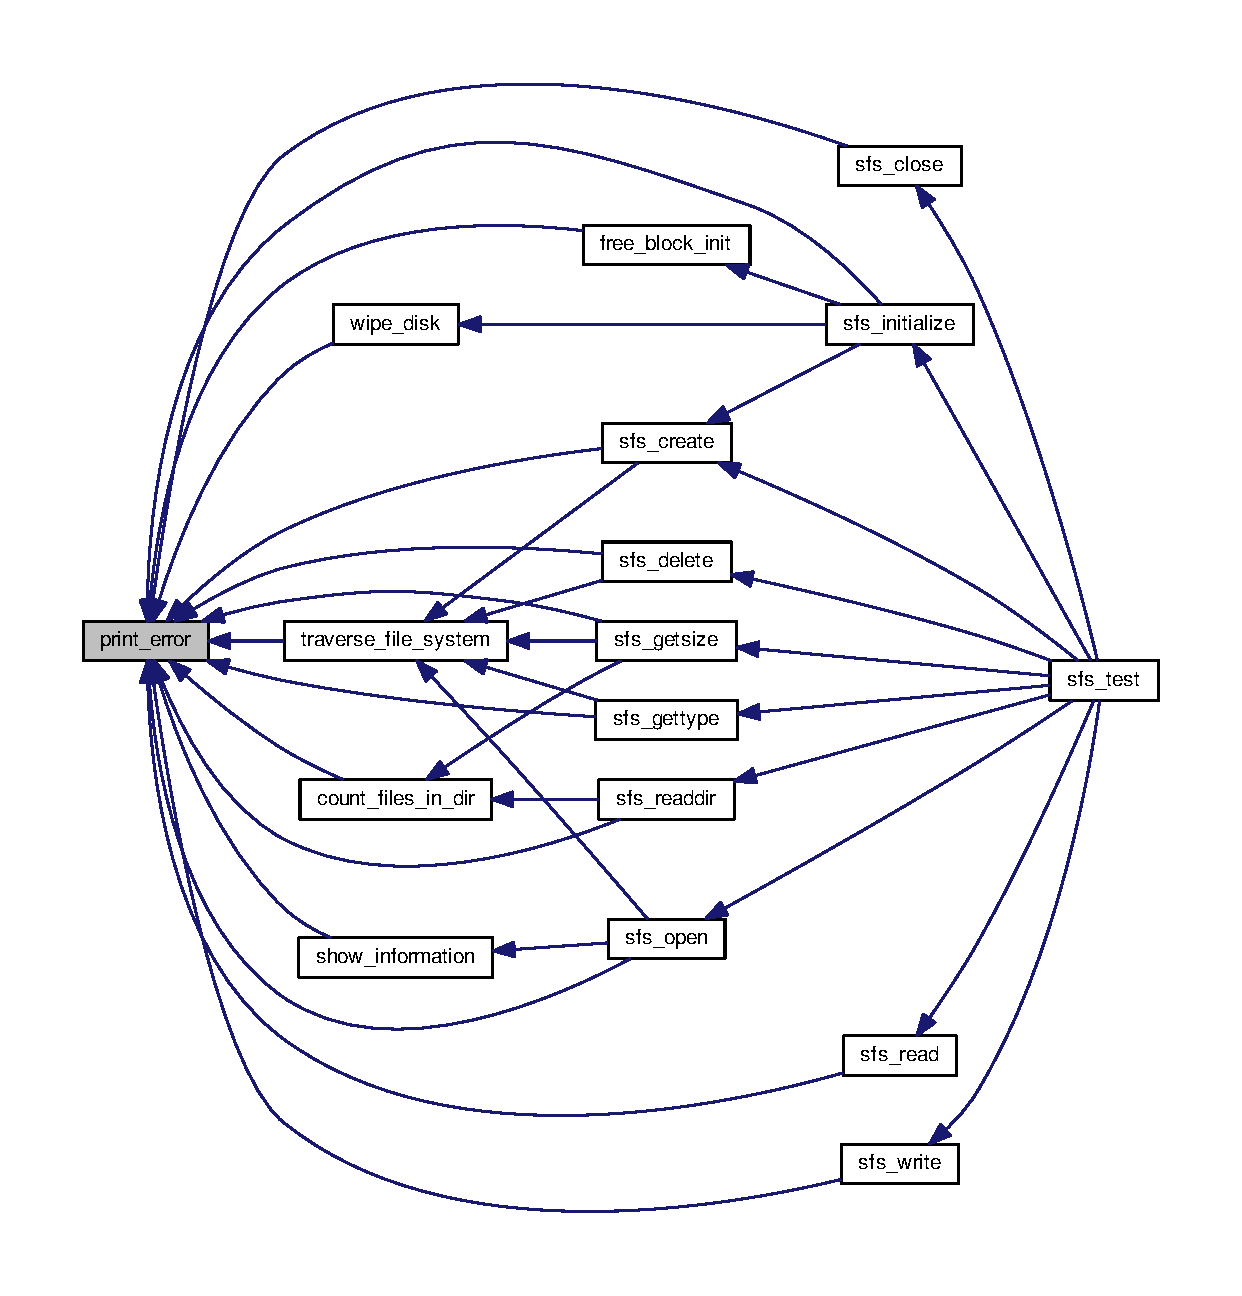
\includegraphics[width=350pt]{error_8c_af85f0519da49c9e50bf3d1feffa74ef3_icgraph}
\end{center}
\end{figure}



\hypertarget{error_8h}{\section{error.\-h File Reference}
\label{error_8h}\index{error.\-h@{error.\-h}}
}
This graph shows which files directly or indirectly include this file\-:
\nopagebreak
\begin{figure}[H]
\begin{center}
\leavevmode
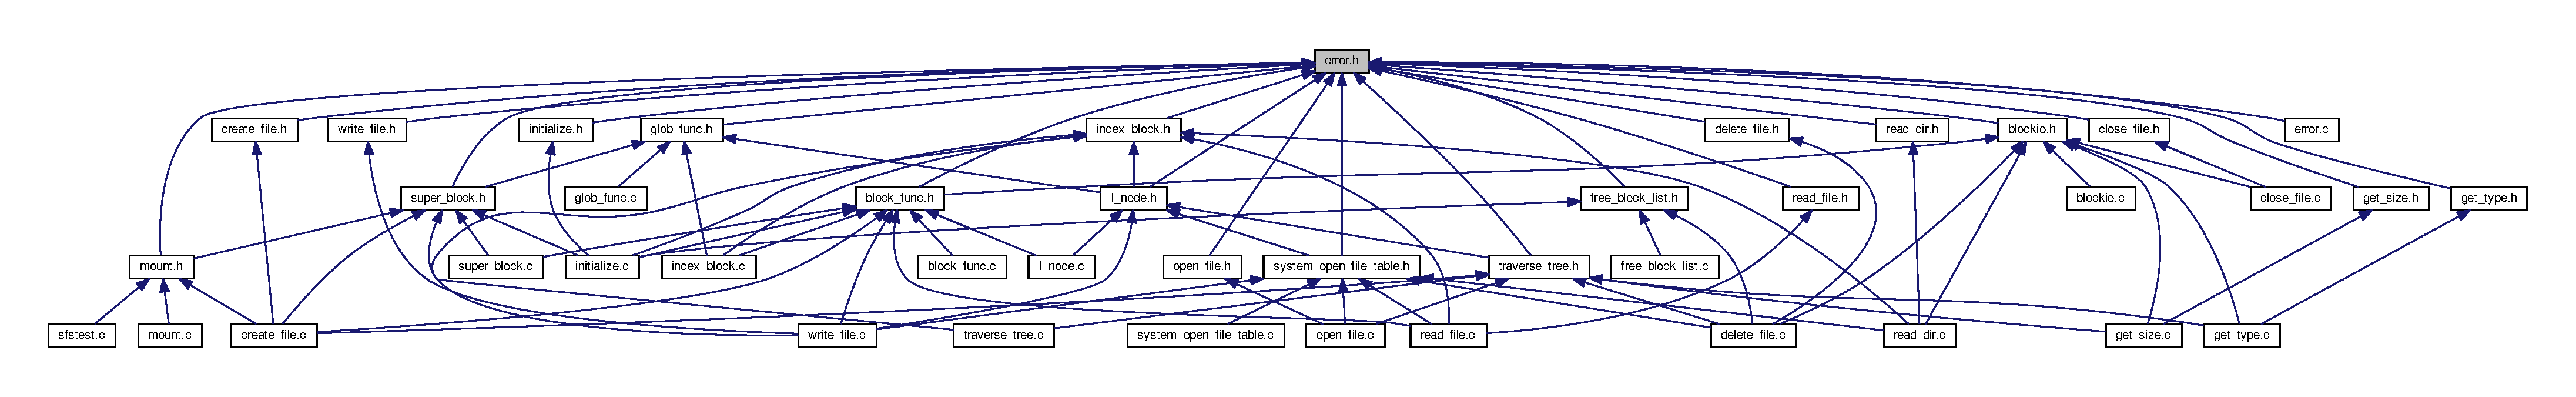
\includegraphics[width=350pt]{error_8h__dep__incl}
\end{center}
\end{figure}
\subsection*{Enumerations}
\begin{DoxyCompactItemize}
\item 
enum \hyperlink{error_8h_a88a76ee847c844cc47b94caac600689d}{error\-\_\-code} \{ \\*
\hyperlink{error_8h_a88a76ee847c844cc47b94caac600689dac7f69f7c9e5aea9b8f54cf02870e2bf8}{S\-U\-C\-C\-E\-S\-S}, 
\hyperlink{error_8h_a88a76ee847c844cc47b94caac600689da0d213a9ce640867b78937ff030c6c76f}{I\-N\-V\-A\-L\-I\-D\-\_\-\-P\-A\-R\-A\-M\-E\-T\-E\-R}, 
\hyperlink{error_8h_a88a76ee847c844cc47b94caac600689dac7423c1a3acae4d7df0445f2c26a7c3a}{D\-I\-S\-K\-\_\-\-R\-E\-A\-D\-\_\-\-E\-R\-R\-O\-R}, 
\hyperlink{error_8h_a88a76ee847c844cc47b94caac600689da514db025322a6b11b789afb8e6c71185}{D\-I\-S\-K\-\_\-\-W\-R\-I\-T\-E\-\_\-\-E\-R\-R\-O\-R}, 
\\*
\hyperlink{error_8h_a88a76ee847c844cc47b94caac600689dabc27a6b909296003973e169faf52f52d}{F\-I\-L\-E\-\_\-\-N\-O\-T\-\_\-\-F\-O\-U\-N\-D}, 
\hyperlink{error_8h_a88a76ee847c844cc47b94caac600689dae4a3e5ca71c2a78a052942e209022823}{I\-N\-V\-A\-L\-I\-D\-\_\-\-F\-I\-L\-E\-\_\-\-T\-Y\-P\-E}, 
\hyperlink{error_8h_a88a76ee847c844cc47b94caac600689da5bd12c3506a0cd6b0b44e585a62d09bc}{I\-N\-V\-A\-L\-I\-D\-\_\-\-F\-I\-L\-E\-\_\-\-N\-A\-M\-E}, 
\hyperlink{error_8h_a88a76ee847c844cc47b94caac600689dac06646da8ff920852222236c9b2e5f9a}{I\-N\-V\-A\-L\-I\-D\-\_\-\-F\-I\-L\-E\-\_\-\-D\-E\-S\-C\-R\-I\-P\-T\-O\-R}, 
\\*
\hyperlink{error_8h_a88a76ee847c844cc47b94caac600689da65c8ffdd83b744c8685263689ab8043e}{I\-N\-V\-A\-L\-I\-D\-\_\-\-P\-A\-T\-H}, 
\hyperlink{error_8h_a88a76ee847c844cc47b94caac600689dafbe0cb7d86b9208a280a5ad930428a01}{I\-N\-V\-A\-L\-I\-D\-\_\-\-P\-A\-T\-H\-\_\-\-L\-E\-N\-G\-T\-H}, 
\hyperlink{error_8h_a88a76ee847c844cc47b94caac600689da54c5aa0c8b218cd4c010d2c915b561f4}{I\-N\-S\-U\-F\-F\-I\-C\-I\-E\-N\-T\-\_\-\-D\-I\-S\-K\-\_\-\-S\-P\-A\-C\-E}, 
\hyperlink{error_8h_a88a76ee847c844cc47b94caac600689dacd19bd5a1cb3a9df7e6a3eaf557a898e}{E\-R\-R\-O\-R\-\_\-\-U\-P\-D\-A\-T\-I\-N\-G\-\_\-\-S\-B}, 
\\*
\hyperlink{error_8h_a88a76ee847c844cc47b94caac600689dafdbfbc759615a99c2cdae1cc0dfaf475}{E\-R\-R\-O\-R\-\_\-\-U\-P\-D\-A\-T\-I\-N\-G\-\_\-\-F\-B\-L}, 
\hyperlink{error_8h_a88a76ee847c844cc47b94caac600689dacf7732724fc12961b476d4dea21275bc}{E\-R\-R\-O\-R\-\_\-\-U\-P\-D\-A\-T\-I\-N\-G\-\_\-\-S\-W\-O\-F\-T}, 
\hyperlink{error_8h_a88a76ee847c844cc47b94caac600689dafb262c03b590ee38c8acb1fbc0051ab2}{I\-N\-D\-E\-X\-\_\-\-A\-L\-L\-O\-C\-A\-T\-I\-O\-N\-\_\-\-E\-R\-R\-O\-R}, 
\hyperlink{error_8h_a88a76ee847c844cc47b94caac600689dadc41a76a2e78602c027c84ffc21b5010}{E\-R\-R\-O\-R\-\_\-\-B\-L\-O\-C\-K\-\_\-\-L\-I\-N\-K\-A\-G\-E}, 
\\*
\hyperlink{error_8h_a88a76ee847c844cc47b94caac600689da0ecf48dbd2620ec31a966358547fc53d}{E\-R\-R\-O\-R\-\_\-\-B\-U\-F\-F\-E\-R\-\_\-\-S\-E\-G\-M\-E\-N\-T\-A\-T\-I\-O\-N}, 
\hyperlink{error_8h_a88a76ee847c844cc47b94caac600689dafd61a993bc2aefbef69725fa2ec04446}{P\-A\-R\-E\-N\-T\-\_\-\-N\-O\-T\-\_\-\-F\-O\-U\-N\-D}, 
\hyperlink{error_8h_a88a76ee847c844cc47b94caac600689da8972a28296ecb5df00bcea7fc05a67f0}{D\-I\-R\-E\-C\-T\-O\-R\-Y\-\_\-\-H\-A\-S\-\_\-\-C\-H\-I\-L\-D\-R\-E\-N}, 
\hyperlink{error_8h_a88a76ee847c844cc47b94caac600689dab22aa0f539397ce8dc3631fec3d542ff}{D\-I\-R\-E\-C\-T\-O\-R\-Y\-\_\-\-T\-R\-A\-V\-E\-R\-S\-E\-D}, 
\\*
\hyperlink{error_8h_a88a76ee847c844cc47b94caac600689da1b9f57411cba62a97c6503b9ce5f6eaf}{D\-I\-R\-E\-C\-T\-O\-R\-Y\-\_\-\-E\-M\-P\-T\-Y}, 
\hyperlink{error_8h_a88a76ee847c844cc47b94caac600689daa83d74fa51c77a952b92c377559965d2}{F\-I\-L\-E\-\_\-\-E\-M\-P\-T\-Y}, 
\hyperlink{error_8h_a88a76ee847c844cc47b94caac600689daa4aaf445712ae638679cb57e79297b87}{F\-I\-L\-E\-\_\-\-P\-A\-S\-T\-\_\-\-E\-O\-F}, 
\hyperlink{error_8h_a88a76ee847c844cc47b94caac600689da6ce26a62afab55d7606ad4e92428b30c}{U\-N\-K\-N\-O\-W\-N}
 \}
\begin{DoxyCompactList}\small\item\em List of error codes with name definitions. \end{DoxyCompactList}\end{DoxyCompactItemize}
\subsection*{Functions}
\begin{DoxyCompactItemize}
\item 
void \hyperlink{error_8h_af85f0519da49c9e50bf3d1feffa74ef3}{print\-\_\-error} (\hyperlink{error_8h_a88a76ee847c844cc47b94caac600689d}{error\-\_\-code} errorno)
\begin{DoxyCompactList}\small\item\em Prints an error code. \end{DoxyCompactList}\end{DoxyCompactItemize}


\subsection{Enumeration Type Documentation}
\hypertarget{error_8h_a88a76ee847c844cc47b94caac600689d}{\index{error.\-h@{error.\-h}!error\-\_\-code@{error\-\_\-code}}
\index{error\-\_\-code@{error\-\_\-code}!error.h@{error.\-h}}
\subsubsection[{error\-\_\-code}]{\setlength{\rightskip}{0pt plus 5cm}enum {\bf error\-\_\-code}}}\label{error_8h_a88a76ee847c844cc47b94caac600689d}


List of error codes with name definitions. 

Contains a list of constant integers used as error codes with a human-\/readable name definitions.

\begin{DoxyAuthor}{Author}
Daniel Smullen

Jonathan Gillett

Joseph Heron
\end{DoxyAuthor}
\begin{DoxyCopyright}{Copyright}
G\-N\-U General Public License V3 
\end{DoxyCopyright}
\begin{Desc}
\item[Enumerator\-: ]\par
\begin{description}
\index{S\-U\-C\-C\-E\-S\-S@{S\-U\-C\-C\-E\-S\-S}!error.\-h@{error.\-h}}\index{error.\-h@{error.\-h}!S\-U\-C\-C\-E\-S\-S@{S\-U\-C\-C\-E\-S\-S}}\item[{\em 
\hypertarget{error_8h_a88a76ee847c844cc47b94caac600689dac7f69f7c9e5aea9b8f54cf02870e2bf8}{S\-U\-C\-C\-E\-S\-S}\label{error_8h_a88a76ee847c844cc47b94caac600689dac7f69f7c9e5aea9b8f54cf02870e2bf8}
}]No error occurred, execution was successful. \index{I\-N\-V\-A\-L\-I\-D\-\_\-\-P\-A\-R\-A\-M\-E\-T\-E\-R@{I\-N\-V\-A\-L\-I\-D\-\_\-\-P\-A\-R\-A\-M\-E\-T\-E\-R}!error.\-h@{error.\-h}}\index{error.\-h@{error.\-h}!I\-N\-V\-A\-L\-I\-D\-\_\-\-P\-A\-R\-A\-M\-E\-T\-E\-R@{I\-N\-V\-A\-L\-I\-D\-\_\-\-P\-A\-R\-A\-M\-E\-T\-E\-R}}\item[{\em 
\hypertarget{error_8h_a88a76ee847c844cc47b94caac600689da0d213a9ce640867b78937ff030c6c76f}{I\-N\-V\-A\-L\-I\-D\-\_\-\-P\-A\-R\-A\-M\-E\-T\-E\-R}\label{error_8h_a88a76ee847c844cc47b94caac600689da0d213a9ce640867b78937ff030c6c76f}
}]An invalid parameter was given to the function. \index{D\-I\-S\-K\-\_\-\-R\-E\-A\-D\-\_\-\-E\-R\-R\-O\-R@{D\-I\-S\-K\-\_\-\-R\-E\-A\-D\-\_\-\-E\-R\-R\-O\-R}!error.\-h@{error.\-h}}\index{error.\-h@{error.\-h}!D\-I\-S\-K\-\_\-\-R\-E\-A\-D\-\_\-\-E\-R\-R\-O\-R@{D\-I\-S\-K\-\_\-\-R\-E\-A\-D\-\_\-\-E\-R\-R\-O\-R}}\item[{\em 
\hypertarget{error_8h_a88a76ee847c844cc47b94caac600689dac7423c1a3acae4d7df0445f2c26a7c3a}{D\-I\-S\-K\-\_\-\-R\-E\-A\-D\-\_\-\-E\-R\-R\-O\-R}\label{error_8h_a88a76ee847c844cc47b94caac600689dac7423c1a3acae4d7df0445f2c26a7c3a}
}]A block of data could not be read from disk. \index{D\-I\-S\-K\-\_\-\-W\-R\-I\-T\-E\-\_\-\-E\-R\-R\-O\-R@{D\-I\-S\-K\-\_\-\-W\-R\-I\-T\-E\-\_\-\-E\-R\-R\-O\-R}!error.\-h@{error.\-h}}\index{error.\-h@{error.\-h}!D\-I\-S\-K\-\_\-\-W\-R\-I\-T\-E\-\_\-\-E\-R\-R\-O\-R@{D\-I\-S\-K\-\_\-\-W\-R\-I\-T\-E\-\_\-\-E\-R\-R\-O\-R}}\item[{\em 
\hypertarget{error_8h_a88a76ee847c844cc47b94caac600689da514db025322a6b11b789afb8e6c71185}{D\-I\-S\-K\-\_\-\-W\-R\-I\-T\-E\-\_\-\-E\-R\-R\-O\-R}\label{error_8h_a88a76ee847c844cc47b94caac600689da514db025322a6b11b789afb8e6c71185}
}]A block of data could not be written to disk. \index{F\-I\-L\-E\-\_\-\-N\-O\-T\-\_\-\-F\-O\-U\-N\-D@{F\-I\-L\-E\-\_\-\-N\-O\-T\-\_\-\-F\-O\-U\-N\-D}!error.\-h@{error.\-h}}\index{error.\-h@{error.\-h}!F\-I\-L\-E\-\_\-\-N\-O\-T\-\_\-\-F\-O\-U\-N\-D@{F\-I\-L\-E\-\_\-\-N\-O\-T\-\_\-\-F\-O\-U\-N\-D}}\item[{\em 
\hypertarget{error_8h_a88a76ee847c844cc47b94caac600689dabc27a6b909296003973e169faf52f52d}{F\-I\-L\-E\-\_\-\-N\-O\-T\-\_\-\-F\-O\-U\-N\-D}\label{error_8h_a88a76ee847c844cc47b94caac600689dabc27a6b909296003973e169faf52f52d}
}]The specified file could not be found on disk. \index{I\-N\-V\-A\-L\-I\-D\-\_\-\-F\-I\-L\-E\-\_\-\-T\-Y\-P\-E@{I\-N\-V\-A\-L\-I\-D\-\_\-\-F\-I\-L\-E\-\_\-\-T\-Y\-P\-E}!error.\-h@{error.\-h}}\index{error.\-h@{error.\-h}!I\-N\-V\-A\-L\-I\-D\-\_\-\-F\-I\-L\-E\-\_\-\-T\-Y\-P\-E@{I\-N\-V\-A\-L\-I\-D\-\_\-\-F\-I\-L\-E\-\_\-\-T\-Y\-P\-E}}\item[{\em 
\hypertarget{error_8h_a88a76ee847c844cc47b94caac600689dae4a3e5ca71c2a78a052942e209022823}{I\-N\-V\-A\-L\-I\-D\-\_\-\-F\-I\-L\-E\-\_\-\-T\-Y\-P\-E}\label{error_8h_a88a76ee847c844cc47b94caac600689dae4a3e5ca71c2a78a052942e209022823}
}]The file type specified is invalid. \index{I\-N\-V\-A\-L\-I\-D\-\_\-\-F\-I\-L\-E\-\_\-\-N\-A\-M\-E@{I\-N\-V\-A\-L\-I\-D\-\_\-\-F\-I\-L\-E\-\_\-\-N\-A\-M\-E}!error.\-h@{error.\-h}}\index{error.\-h@{error.\-h}!I\-N\-V\-A\-L\-I\-D\-\_\-\-F\-I\-L\-E\-\_\-\-N\-A\-M\-E@{I\-N\-V\-A\-L\-I\-D\-\_\-\-F\-I\-L\-E\-\_\-\-N\-A\-M\-E}}\item[{\em 
\hypertarget{error_8h_a88a76ee847c844cc47b94caac600689da5bd12c3506a0cd6b0b44e585a62d09bc}{I\-N\-V\-A\-L\-I\-D\-\_\-\-F\-I\-L\-E\-\_\-\-N\-A\-M\-E}\label{error_8h_a88a76ee847c844cc47b94caac600689da5bd12c3506a0cd6b0b44e585a62d09bc}
}]The file name specified is invalid. \index{I\-N\-V\-A\-L\-I\-D\-\_\-\-F\-I\-L\-E\-\_\-\-D\-E\-S\-C\-R\-I\-P\-T\-O\-R@{I\-N\-V\-A\-L\-I\-D\-\_\-\-F\-I\-L\-E\-\_\-\-D\-E\-S\-C\-R\-I\-P\-T\-O\-R}!error.\-h@{error.\-h}}\index{error.\-h@{error.\-h}!I\-N\-V\-A\-L\-I\-D\-\_\-\-F\-I\-L\-E\-\_\-\-D\-E\-S\-C\-R\-I\-P\-T\-O\-R@{I\-N\-V\-A\-L\-I\-D\-\_\-\-F\-I\-L\-E\-\_\-\-D\-E\-S\-C\-R\-I\-P\-T\-O\-R}}\item[{\em 
\hypertarget{error_8h_a88a76ee847c844cc47b94caac600689dac06646da8ff920852222236c9b2e5f9a}{I\-N\-V\-A\-L\-I\-D\-\_\-\-F\-I\-L\-E\-\_\-\-D\-E\-S\-C\-R\-I\-P\-T\-O\-R}\label{error_8h_a88a76ee847c844cc47b94caac600689dac06646da8ff920852222236c9b2e5f9a}
}]The file descriptor specified is invalid or does not exist. \index{I\-N\-V\-A\-L\-I\-D\-\_\-\-P\-A\-T\-H@{I\-N\-V\-A\-L\-I\-D\-\_\-\-P\-A\-T\-H}!error.\-h@{error.\-h}}\index{error.\-h@{error.\-h}!I\-N\-V\-A\-L\-I\-D\-\_\-\-P\-A\-T\-H@{I\-N\-V\-A\-L\-I\-D\-\_\-\-P\-A\-T\-H}}\item[{\em 
\hypertarget{error_8h_a88a76ee847c844cc47b94caac600689da65c8ffdd83b744c8685263689ab8043e}{I\-N\-V\-A\-L\-I\-D\-\_\-\-P\-A\-T\-H}\label{error_8h_a88a76ee847c844cc47b94caac600689da65c8ffdd83b744c8685263689ab8043e}
}]The path specified is invalid. \index{I\-N\-V\-A\-L\-I\-D\-\_\-\-P\-A\-T\-H\-\_\-\-L\-E\-N\-G\-T\-H@{I\-N\-V\-A\-L\-I\-D\-\_\-\-P\-A\-T\-H\-\_\-\-L\-E\-N\-G\-T\-H}!error.\-h@{error.\-h}}\index{error.\-h@{error.\-h}!I\-N\-V\-A\-L\-I\-D\-\_\-\-P\-A\-T\-H\-\_\-\-L\-E\-N\-G\-T\-H@{I\-N\-V\-A\-L\-I\-D\-\_\-\-P\-A\-T\-H\-\_\-\-L\-E\-N\-G\-T\-H}}\item[{\em 
\hypertarget{error_8h_a88a76ee847c844cc47b94caac600689dafbe0cb7d86b9208a280a5ad930428a01}{I\-N\-V\-A\-L\-I\-D\-\_\-\-P\-A\-T\-H\-\_\-\-L\-E\-N\-G\-T\-H}\label{error_8h_a88a76ee847c844cc47b94caac600689dafbe0cb7d86b9208a280a5ad930428a01}
}]The path length given is too long, path tokens cannot be longer than 6 characters. \index{I\-N\-S\-U\-F\-F\-I\-C\-I\-E\-N\-T\-\_\-\-D\-I\-S\-K\-\_\-\-S\-P\-A\-C\-E@{I\-N\-S\-U\-F\-F\-I\-C\-I\-E\-N\-T\-\_\-\-D\-I\-S\-K\-\_\-\-S\-P\-A\-C\-E}!error.\-h@{error.\-h}}\index{error.\-h@{error.\-h}!I\-N\-S\-U\-F\-F\-I\-C\-I\-E\-N\-T\-\_\-\-D\-I\-S\-K\-\_\-\-S\-P\-A\-C\-E@{I\-N\-S\-U\-F\-F\-I\-C\-I\-E\-N\-T\-\_\-\-D\-I\-S\-K\-\_\-\-S\-P\-A\-C\-E}}\item[{\em 
\hypertarget{error_8h_a88a76ee847c844cc47b94caac600689da54c5aa0c8b218cd4c010d2c915b561f4}{I\-N\-S\-U\-F\-F\-I\-C\-I\-E\-N\-T\-\_\-\-D\-I\-S\-K\-\_\-\-S\-P\-A\-C\-E}\label{error_8h_a88a76ee847c844cc47b94caac600689da54c5aa0c8b218cd4c010d2c915b561f4}
}]The requested operation does not have sufficient blocks available on disk to complete execution. \index{E\-R\-R\-O\-R\-\_\-\-U\-P\-D\-A\-T\-I\-N\-G\-\_\-\-S\-B@{E\-R\-R\-O\-R\-\_\-\-U\-P\-D\-A\-T\-I\-N\-G\-\_\-\-S\-B}!error.\-h@{error.\-h}}\index{error.\-h@{error.\-h}!E\-R\-R\-O\-R\-\_\-\-U\-P\-D\-A\-T\-I\-N\-G\-\_\-\-S\-B@{E\-R\-R\-O\-R\-\_\-\-U\-P\-D\-A\-T\-I\-N\-G\-\_\-\-S\-B}}\item[{\em 
\hypertarget{error_8h_a88a76ee847c844cc47b94caac600689dacd19bd5a1cb3a9df7e6a3eaf557a898e}{E\-R\-R\-O\-R\-\_\-\-U\-P\-D\-A\-T\-I\-N\-G\-\_\-\-S\-B}\label{error_8h_a88a76ee847c844cc47b94caac600689dacd19bd5a1cb3a9df7e6a3eaf557a898e}
}]Fatal error\-: The super block could not be updated. The file system or disk are corrupted. \index{E\-R\-R\-O\-R\-\_\-\-U\-P\-D\-A\-T\-I\-N\-G\-\_\-\-F\-B\-L@{E\-R\-R\-O\-R\-\_\-\-U\-P\-D\-A\-T\-I\-N\-G\-\_\-\-F\-B\-L}!error.\-h@{error.\-h}}\index{error.\-h@{error.\-h}!E\-R\-R\-O\-R\-\_\-\-U\-P\-D\-A\-T\-I\-N\-G\-\_\-\-F\-B\-L@{E\-R\-R\-O\-R\-\_\-\-U\-P\-D\-A\-T\-I\-N\-G\-\_\-\-F\-B\-L}}\item[{\em 
\hypertarget{error_8h_a88a76ee847c844cc47b94caac600689dafdbfbc759615a99c2cdae1cc0dfaf475}{E\-R\-R\-O\-R\-\_\-\-U\-P\-D\-A\-T\-I\-N\-G\-\_\-\-F\-B\-L}\label{error_8h_a88a76ee847c844cc47b94caac600689dafdbfbc759615a99c2cdae1cc0dfaf475}
}]Fatal error\-: The free block list could not be updated. The file system or disk may be corrupted. \index{E\-R\-R\-O\-R\-\_\-\-U\-P\-D\-A\-T\-I\-N\-G\-\_\-\-S\-W\-O\-F\-T@{E\-R\-R\-O\-R\-\_\-\-U\-P\-D\-A\-T\-I\-N\-G\-\_\-\-S\-W\-O\-F\-T}!error.\-h@{error.\-h}}\index{error.\-h@{error.\-h}!E\-R\-R\-O\-R\-\_\-\-U\-P\-D\-A\-T\-I\-N\-G\-\_\-\-S\-W\-O\-F\-T@{E\-R\-R\-O\-R\-\_\-\-U\-P\-D\-A\-T\-I\-N\-G\-\_\-\-S\-W\-O\-F\-T}}\item[{\em 
\hypertarget{error_8h_a88a76ee847c844cc47b94caac600689dacf7732724fc12961b476d4dea21275bc}{E\-R\-R\-O\-R\-\_\-\-U\-P\-D\-A\-T\-I\-N\-G\-\_\-\-S\-W\-O\-F\-T}\label{error_8h_a88a76ee847c844cc47b94caac600689dacf7732724fc12961b476d4dea21275bc}
}]The system-\/wide open file table cannot be updated. This may be indicative of memory corruption. \index{I\-N\-D\-E\-X\-\_\-\-A\-L\-L\-O\-C\-A\-T\-I\-O\-N\-\_\-\-E\-R\-R\-O\-R@{I\-N\-D\-E\-X\-\_\-\-A\-L\-L\-O\-C\-A\-T\-I\-O\-N\-\_\-\-E\-R\-R\-O\-R}!error.\-h@{error.\-h}}\index{error.\-h@{error.\-h}!I\-N\-D\-E\-X\-\_\-\-A\-L\-L\-O\-C\-A\-T\-I\-O\-N\-\_\-\-E\-R\-R\-O\-R@{I\-N\-D\-E\-X\-\_\-\-A\-L\-L\-O\-C\-A\-T\-I\-O\-N\-\_\-\-E\-R\-R\-O\-R}}\item[{\em 
\hypertarget{error_8h_a88a76ee847c844cc47b94caac600689dafb262c03b590ee38c8acb1fbc0051ab2}{I\-N\-D\-E\-X\-\_\-\-A\-L\-L\-O\-C\-A\-T\-I\-O\-N\-\_\-\-E\-R\-R\-O\-R}\label{error_8h_a88a76ee847c844cc47b94caac600689dafb262c03b590ee38c8acb1fbc0051ab2}
}]The given index block data structure is corrupted, invalid, or empty. \index{E\-R\-R\-O\-R\-\_\-\-B\-L\-O\-C\-K\-\_\-\-L\-I\-N\-K\-A\-G\-E@{E\-R\-R\-O\-R\-\_\-\-B\-L\-O\-C\-K\-\_\-\-L\-I\-N\-K\-A\-G\-E}!error.\-h@{error.\-h}}\index{error.\-h@{error.\-h}!E\-R\-R\-O\-R\-\_\-\-B\-L\-O\-C\-K\-\_\-\-L\-I\-N\-K\-A\-G\-E@{E\-R\-R\-O\-R\-\_\-\-B\-L\-O\-C\-K\-\_\-\-L\-I\-N\-K\-A\-G\-E}}\item[{\em 
\hypertarget{error_8h_a88a76ee847c844cc47b94caac600689dadc41a76a2e78602c027c84ffc21b5010}{E\-R\-R\-O\-R\-\_\-\-B\-L\-O\-C\-K\-\_\-\-L\-I\-N\-K\-A\-G\-E}\label{error_8h_a88a76ee847c844cc47b94caac600689dadc41a76a2e78602c027c84ffc21b5010}
}]An error occurred concerning the linkage of an inode to an index block structure. \index{E\-R\-R\-O\-R\-\_\-\-B\-U\-F\-F\-E\-R\-\_\-\-S\-E\-G\-M\-E\-N\-T\-A\-T\-I\-O\-N@{E\-R\-R\-O\-R\-\_\-\-B\-U\-F\-F\-E\-R\-\_\-\-S\-E\-G\-M\-E\-N\-T\-A\-T\-I\-O\-N}!error.\-h@{error.\-h}}\index{error.\-h@{error.\-h}!E\-R\-R\-O\-R\-\_\-\-B\-U\-F\-F\-E\-R\-\_\-\-S\-E\-G\-M\-E\-N\-T\-A\-T\-I\-O\-N@{E\-R\-R\-O\-R\-\_\-\-B\-U\-F\-F\-E\-R\-\_\-\-S\-E\-G\-M\-E\-N\-T\-A\-T\-I\-O\-N}}\item[{\em 
\hypertarget{error_8h_a88a76ee847c844cc47b94caac600689da0ecf48dbd2620ec31a966358547fc53d}{E\-R\-R\-O\-R\-\_\-\-B\-U\-F\-F\-E\-R\-\_\-\-S\-E\-G\-M\-E\-N\-T\-A\-T\-I\-O\-N}\label{error_8h_a88a76ee847c844cc47b94caac600689da0ecf48dbd2620ec31a966358547fc53d}
}]An error occurred segmenting a buffer into block-\/sized chunks. \index{P\-A\-R\-E\-N\-T\-\_\-\-N\-O\-T\-\_\-\-F\-O\-U\-N\-D@{P\-A\-R\-E\-N\-T\-\_\-\-N\-O\-T\-\_\-\-F\-O\-U\-N\-D}!error.\-h@{error.\-h}}\index{error.\-h@{error.\-h}!P\-A\-R\-E\-N\-T\-\_\-\-N\-O\-T\-\_\-\-F\-O\-U\-N\-D@{P\-A\-R\-E\-N\-T\-\_\-\-N\-O\-T\-\_\-\-F\-O\-U\-N\-D}}\item[{\em 
\hypertarget{error_8h_a88a76ee847c844cc47b94caac600689dafd61a993bc2aefbef69725fa2ec04446}{P\-A\-R\-E\-N\-T\-\_\-\-N\-O\-T\-\_\-\-F\-O\-U\-N\-D}\label{error_8h_a88a76ee847c844cc47b94caac600689dafd61a993bc2aefbef69725fa2ec04446}
}]An inode has become loose, and its parent cannot be found. \index{D\-I\-R\-E\-C\-T\-O\-R\-Y\-\_\-\-H\-A\-S\-\_\-\-C\-H\-I\-L\-D\-R\-E\-N@{D\-I\-R\-E\-C\-T\-O\-R\-Y\-\_\-\-H\-A\-S\-\_\-\-C\-H\-I\-L\-D\-R\-E\-N}!error.\-h@{error.\-h}}\index{error.\-h@{error.\-h}!D\-I\-R\-E\-C\-T\-O\-R\-Y\-\_\-\-H\-A\-S\-\_\-\-C\-H\-I\-L\-D\-R\-E\-N@{D\-I\-R\-E\-C\-T\-O\-R\-Y\-\_\-\-H\-A\-S\-\_\-\-C\-H\-I\-L\-D\-R\-E\-N}}\item[{\em 
\hypertarget{error_8h_a88a76ee847c844cc47b94caac600689da8972a28296ecb5df00bcea7fc05a67f0}{D\-I\-R\-E\-C\-T\-O\-R\-Y\-\_\-\-H\-A\-S\-\_\-\-C\-H\-I\-L\-D\-R\-E\-N}\label{error_8h_a88a76ee847c844cc47b94caac600689da8972a28296ecb5df00bcea7fc05a67f0}
}]An attempt was made to delete a directory which has children. Directories must be empty to be deleted. \index{D\-I\-R\-E\-C\-T\-O\-R\-Y\-\_\-\-T\-R\-A\-V\-E\-R\-S\-E\-D@{D\-I\-R\-E\-C\-T\-O\-R\-Y\-\_\-\-T\-R\-A\-V\-E\-R\-S\-E\-D}!error.\-h@{error.\-h}}\index{error.\-h@{error.\-h}!D\-I\-R\-E\-C\-T\-O\-R\-Y\-\_\-\-T\-R\-A\-V\-E\-R\-S\-E\-D@{D\-I\-R\-E\-C\-T\-O\-R\-Y\-\_\-\-T\-R\-A\-V\-E\-R\-S\-E\-D}}\item[{\em 
\hypertarget{error_8h_a88a76ee847c844cc47b94caac600689dab22aa0f539397ce8dc3631fec3d542ff}{D\-I\-R\-E\-C\-T\-O\-R\-Y\-\_\-\-T\-R\-A\-V\-E\-R\-S\-E\-D}\label{error_8h_a88a76ee847c844cc47b94caac600689dab22aa0f539397ce8dc3631fec3d542ff}
}]A directory was fully traversed. Further attempts to read the contents of the directory will begin from the top of the structure. \index{D\-I\-R\-E\-C\-T\-O\-R\-Y\-\_\-\-E\-M\-P\-T\-Y@{D\-I\-R\-E\-C\-T\-O\-R\-Y\-\_\-\-E\-M\-P\-T\-Y}!error.\-h@{error.\-h}}\index{error.\-h@{error.\-h}!D\-I\-R\-E\-C\-T\-O\-R\-Y\-\_\-\-E\-M\-P\-T\-Y@{D\-I\-R\-E\-C\-T\-O\-R\-Y\-\_\-\-E\-M\-P\-T\-Y}}\item[{\em 
\hypertarget{error_8h_a88a76ee847c844cc47b94caac600689da1b9f57411cba62a97c6503b9ce5f6eaf}{D\-I\-R\-E\-C\-T\-O\-R\-Y\-\_\-\-E\-M\-P\-T\-Y}\label{error_8h_a88a76ee847c844cc47b94caac600689da1b9f57411cba62a97c6503b9ce5f6eaf}
}]An attempt was made to read the contents of an empty directory. \index{F\-I\-L\-E\-\_\-\-E\-M\-P\-T\-Y@{F\-I\-L\-E\-\_\-\-E\-M\-P\-T\-Y}!error.\-h@{error.\-h}}\index{error.\-h@{error.\-h}!F\-I\-L\-E\-\_\-\-E\-M\-P\-T\-Y@{F\-I\-L\-E\-\_\-\-E\-M\-P\-T\-Y}}\item[{\em 
\hypertarget{error_8h_a88a76ee847c844cc47b94caac600689daa83d74fa51c77a952b92c377559965d2}{F\-I\-L\-E\-\_\-\-E\-M\-P\-T\-Y}\label{error_8h_a88a76ee847c844cc47b94caac600689daa83d74fa51c77a952b92c377559965d2}
}]An attempt was made to perform operations on a file which contains no data. \index{F\-I\-L\-E\-\_\-\-P\-A\-S\-T\-\_\-\-E\-O\-F@{F\-I\-L\-E\-\_\-\-P\-A\-S\-T\-\_\-\-E\-O\-F}!error.\-h@{error.\-h}}\index{error.\-h@{error.\-h}!F\-I\-L\-E\-\_\-\-P\-A\-S\-T\-\_\-\-E\-O\-F@{F\-I\-L\-E\-\_\-\-P\-A\-S\-T\-\_\-\-E\-O\-F}}\item[{\em 
\hypertarget{error_8h_a88a76ee847c844cc47b94caac600689daa4aaf445712ae638679cb57e79297b87}{F\-I\-L\-E\-\_\-\-P\-A\-S\-T\-\_\-\-E\-O\-F}\label{error_8h_a88a76ee847c844cc47b94caac600689daa4aaf445712ae638679cb57e79297b87}
}]An attempt was made to write to a file past the current length of the file, without appending. Appending is the only allowed way to increase the length of a file. \index{U\-N\-K\-N\-O\-W\-N@{U\-N\-K\-N\-O\-W\-N}!error.\-h@{error.\-h}}\index{error.\-h@{error.\-h}!U\-N\-K\-N\-O\-W\-N@{U\-N\-K\-N\-O\-W\-N}}\item[{\em 
\hypertarget{error_8h_a88a76ee847c844cc47b94caac600689da6ce26a62afab55d7606ad4e92428b30c}{U\-N\-K\-N\-O\-W\-N}\label{error_8h_a88a76ee847c844cc47b94caac600689da6ce26a62afab55d7606ad4e92428b30c}
}]An unknown error occurred. \end{description}
\end{Desc}



\subsection{Function Documentation}
\hypertarget{error_8h_af85f0519da49c9e50bf3d1feffa74ef3}{\index{error.\-h@{error.\-h}!print\-\_\-error@{print\-\_\-error}}
\index{print\-\_\-error@{print\-\_\-error}!error.h@{error.\-h}}
\subsubsection[{print\-\_\-error}]{\setlength{\rightskip}{0pt plus 5cm}void print\-\_\-error (
\begin{DoxyParamCaption}
\item[{{\bf error\-\_\-code}}]{errorno}
\end{DoxyParamCaption}
)}}\label{error_8h_af85f0519da49c9e50bf3d1feffa74ef3}


Prints an error code. 

Outputs the specified error code to the console. Fatal errors will cause the application to terminate immediately to prevent file system or disk corruption.


\begin{DoxyParams}{Parameters}
{\em The} & specified error to output.\\
\hline
\end{DoxyParams}
\begin{DoxyAuthor}{Author}
Daniel Smullen

Jonathan Gillett

Joseph Heron
\end{DoxyAuthor}
\begin{DoxyCopyright}{Copyright}
G\-N\-U General Public License V3 
\end{DoxyCopyright}


Here is the caller graph for this function\-:
\nopagebreak
\begin{figure}[H]
\begin{center}
\leavevmode
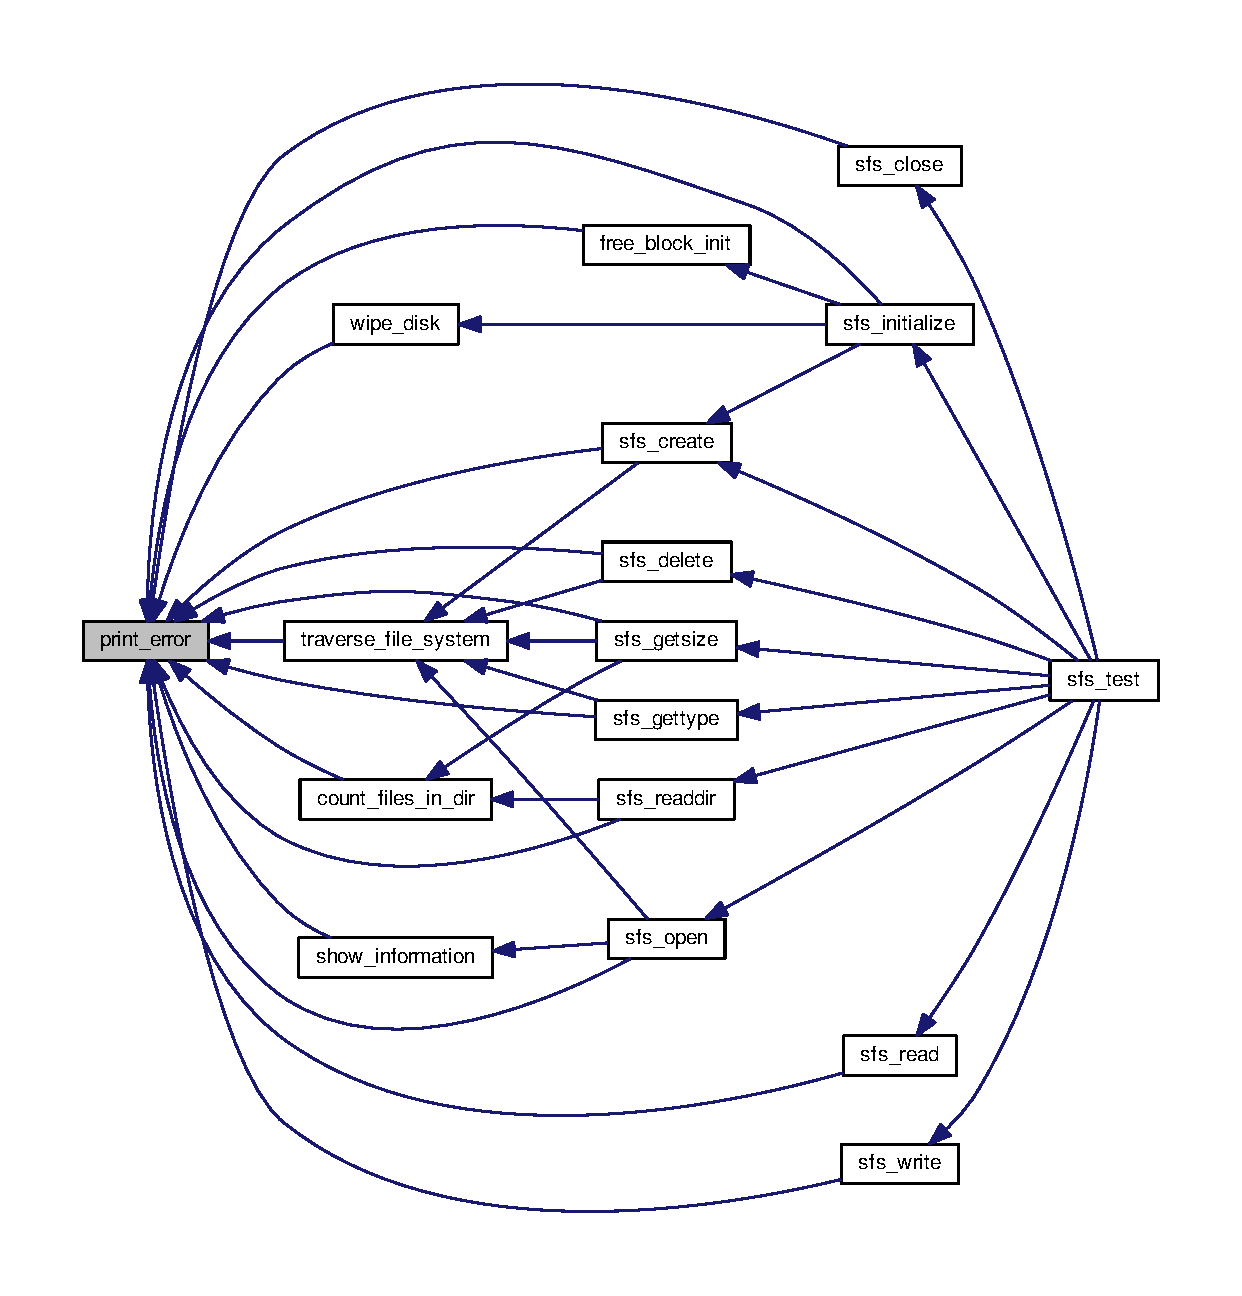
\includegraphics[width=350pt]{error_8h_af85f0519da49c9e50bf3d1feffa74ef3_icgraph}
\end{center}
\end{figure}



\hypertarget{free__block__list_8c}{\section{free\-\_\-block\-\_\-list.\-c File Reference}
\label{free__block__list_8c}\index{free\-\_\-block\-\_\-list.\-c@{free\-\_\-block\-\_\-list.\-c}}
}
{\ttfamily \#include \char`\"{}free\-\_\-block\-\_\-list.\-h\char`\"{}}\\*
{\ttfamily \#include $<$stdbool.\-h$>$}\\*
Include dependency graph for free\-\_\-block\-\_\-list.\-c\-:
\nopagebreak
\begin{figure}[H]
\begin{center}
\leavevmode
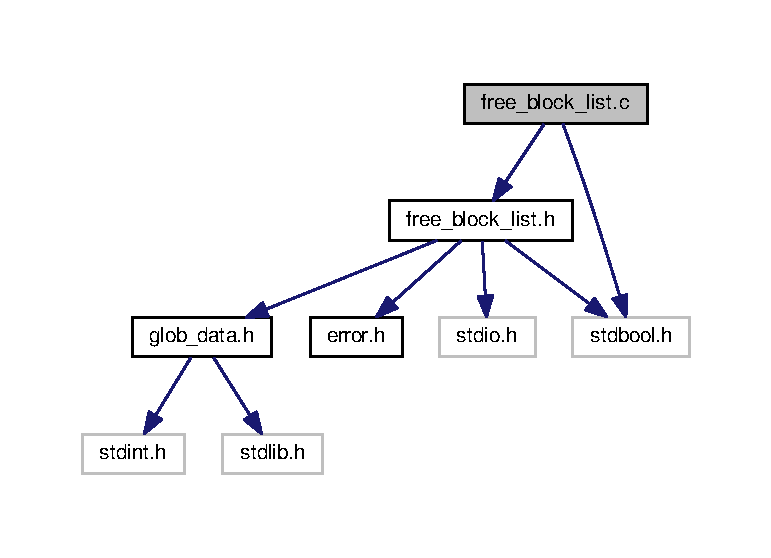
\includegraphics[width=350pt]{free__block__list_8c__incl}
\end{center}
\end{figure}
\subsection*{Functions}
\begin{DoxyCompactItemize}
\item 
\hyperlink{structfree__block__list}{free\-\_\-block\-\_\-list} $\ast$ \hyperlink{free__block__list_8c_a4fb9e58d343f5d00bfddf8b2aabe4a05}{get\-\_\-free\-\_\-block\-\_\-list} (void)
\begin{DoxyCompactList}\small\item\em Obtains a handle to the free block list static instance, regardless of whether it is available in memory or on disk. \end{DoxyCompactList}\item 
\hyperlink{glob__data_8h_a9d4937e46b9fac69334d5fc7ea3f37a6}{locations} \hyperlink{free__block__list_8c_a4006c8928b03cc8367e345842cd263ae}{calc\-\_\-total\-\_\-free\-\_\-blocks} (void)
\begin{DoxyCompactList}\small\item\em Used to calculate the total amount of available disk space. \end{DoxyCompactList}\item 
\hyperlink{glob__data_8h_a9d4937e46b9fac69334d5fc7ea3f37a6}{locations} \hyperlink{free__block__list_8c_a82bb5a646a9f221b4b1b333cd1e142ea}{calc\-\_\-num\-\_\-free\-\_\-blocks} (uint32\-\_\-t num\-\_\-blocks)
\begin{DoxyCompactList}\small\item\em Used to calculate whether there is enough disk space before starting to create a file on disk. \end{DoxyCompactList}\item 
uint32\-\_\-t \hyperlink{free__block__list_8c_acbfc0a3810742af6e976d135071261e1}{get\-\_\-free\-\_\-block} (void)
\begin{DoxyCompactList}\small\item\em Finds the next free block in the static free block list, marks it as used and returns the location of the block. \end{DoxyCompactList}\item 
\hyperlink{structfree__block__list}{free\-\_\-block\-\_\-list} $\ast$ \hyperlink{free__block__list_8c_adafbfcac2573a9ee6a15645d4fe825c0}{update\-\_\-fbl} (\hyperlink{glob__data_8h_a9d4937e46b9fac69334d5fc7ea3f37a6}{locations} used, \hyperlink{glob__data_8h_a9d4937e46b9fac69334d5fc7ea3f37a6}{locations} free)
\begin{DoxyCompactList}\small\item\em Accessor method for the free block list static instance in memory. \end{DoxyCompactList}\item 
\hyperlink{structfree__block__list}{free\-\_\-block\-\_\-list} $\ast$ \hyperlink{free__block__list_8c_a1a24d3e02317587656b22b7207cdb3fe}{sync\-\_\-fbl} (void)
\begin{DoxyCompactList}\small\item\em Synchronizes the free block static instance in memory by writing it to disk. \end{DoxyCompactList}\item 
\hyperlink{structfree__block__list}{free\-\_\-block\-\_\-list} $\ast$ \hyperlink{free__block__list_8c_ae1a3d63476e1321750e8e4aedbc53f07}{reset\-\_\-fbl} (void)
\begin{DoxyCompactList}\small\item\em Overwrites the free block list in memory with the most recent version on disk. \end{DoxyCompactList}\item 
\hyperlink{structfree__block__list}{free\-\_\-block\-\_\-list} $\ast$ \hyperlink{free__block__list_8c_a9e849ebe5efb8153894a337356a4e328}{wipe\-\_\-fbl} (void)
\begin{DoxyCompactList}\small\item\em Reinitializes the free block list in memory. \end{DoxyCompactList}\end{DoxyCompactItemize}


\subsection{Function Documentation}
\hypertarget{free__block__list_8c_a82bb5a646a9f221b4b1b333cd1e142ea}{\index{free\-\_\-block\-\_\-list.\-c@{free\-\_\-block\-\_\-list.\-c}!calc\-\_\-num\-\_\-free\-\_\-blocks@{calc\-\_\-num\-\_\-free\-\_\-blocks}}
\index{calc\-\_\-num\-\_\-free\-\_\-blocks@{calc\-\_\-num\-\_\-free\-\_\-blocks}!free_block_list.c@{free\-\_\-block\-\_\-list.\-c}}
\subsubsection[{calc\-\_\-num\-\_\-free\-\_\-blocks}]{\setlength{\rightskip}{0pt plus 5cm}{\bf locations} calc\-\_\-num\-\_\-free\-\_\-blocks (
\begin{DoxyParamCaption}
\item[{uint32\-\_\-t}]{num\-\_\-blocks}
\end{DoxyParamCaption}
)}}\label{free__block__list_8c_a82bb5a646a9f221b4b1b333cd1e142ea}


Used to calculate whether there is enough disk space before starting to create a file on disk. 

Finds the specified number of free blocks in the static instance of the free block list in memory. It returns N\-U\-L\-L if there are not enough free blocks, otherwise it returns an array of the free locations.


\begin{DoxyParams}{Parameters}
{\em num\-\_\-blocks} & The number of free blocks needed.\\
\hline
\end{DoxyParams}
\begin{DoxyReturn}{Returns}
Returns an array of the free locations, or N\-U\-L\-L if there are not enough free blocks.
\end{DoxyReturn}
\begin{DoxyAuthor}{Author}
Daniel Smullen

Jonathan Gillett

Joseph Heron
\end{DoxyAuthor}
\begin{DoxyCopyright}{Copyright}
G\-N\-U General Public License V3 
\end{DoxyCopyright}


Here is the caller graph for this function\-:
\nopagebreak
\begin{figure}[H]
\begin{center}
\leavevmode
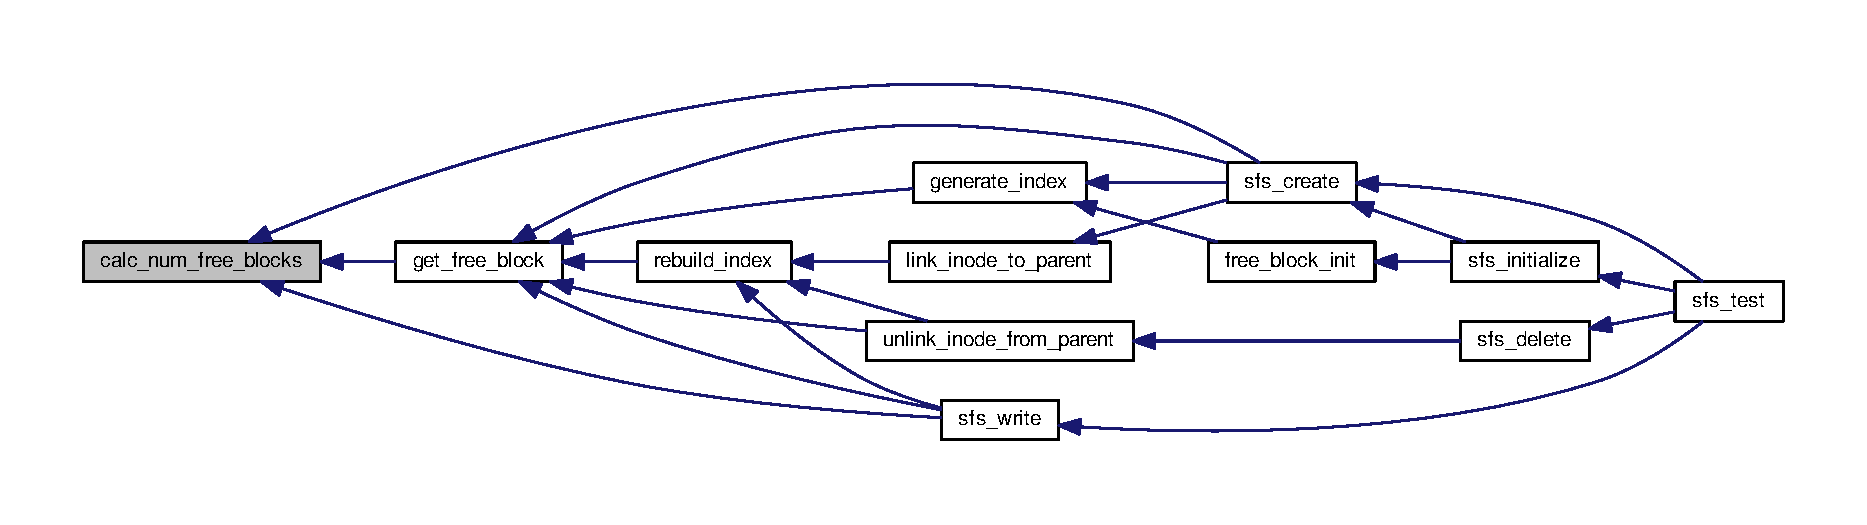
\includegraphics[width=350pt]{free__block__list_8c_a82bb5a646a9f221b4b1b333cd1e142ea_icgraph}
\end{center}
\end{figure}


\hypertarget{free__block__list_8c_a4006c8928b03cc8367e345842cd263ae}{\index{free\-\_\-block\-\_\-list.\-c@{free\-\_\-block\-\_\-list.\-c}!calc\-\_\-total\-\_\-free\-\_\-blocks@{calc\-\_\-total\-\_\-free\-\_\-blocks}}
\index{calc\-\_\-total\-\_\-free\-\_\-blocks@{calc\-\_\-total\-\_\-free\-\_\-blocks}!free_block_list.c@{free\-\_\-block\-\_\-list.\-c}}
\subsubsection[{calc\-\_\-total\-\_\-free\-\_\-blocks}]{\setlength{\rightskip}{0pt plus 5cm}{\bf locations} calc\-\_\-total\-\_\-free\-\_\-blocks (
\begin{DoxyParamCaption}
\item[{void}]{}
\end{DoxyParamCaption}
)}}\label{free__block__list_8c_a4006c8928b03cc8367e345842cd263ae}


Used to calculate the total amount of available disk space. 

Finds all of the free blocks that exist in the static instance of the free block list in memory and returns them as a locations object.

\begin{DoxyReturn}{Returns}
Returns an array containing all of the free locations.
\end{DoxyReturn}
\begin{DoxyAuthor}{Author}
Daniel Smullen

Jonathan Gillett

Joseph Heron
\end{DoxyAuthor}
\begin{DoxyCopyright}{Copyright}
G\-N\-U General Public License V3 
\end{DoxyCopyright}


Here is the caller graph for this function\-:
\nopagebreak
\begin{figure}[H]
\begin{center}
\leavevmode
\includegraphics[width=350pt]{free__block__list_8c_a4006c8928b03cc8367e345842cd263ae_icgraph}
\end{center}
\end{figure}


\hypertarget{free__block__list_8c_acbfc0a3810742af6e976d135071261e1}{\index{free\-\_\-block\-\_\-list.\-c@{free\-\_\-block\-\_\-list.\-c}!get\-\_\-free\-\_\-block@{get\-\_\-free\-\_\-block}}
\index{get\-\_\-free\-\_\-block@{get\-\_\-free\-\_\-block}!free_block_list.c@{free\-\_\-block\-\_\-list.\-c}}
\subsubsection[{get\-\_\-free\-\_\-block}]{\setlength{\rightskip}{0pt plus 5cm}uint32\-\_\-t get\-\_\-free\-\_\-block (
\begin{DoxyParamCaption}
\item[{void}]{}
\end{DoxyParamCaption}
)}}\label{free__block__list_8c_acbfc0a3810742af6e976d135071261e1}


Finds the next free block in the static free block list, marks it as used and returns the location of the block. 

This function finds a single free block and then marks that block as used in the free block list, it ensures that the block on disk is empty (all N\-U\-L\-L) before returning the block location. It essentially operates as a facade for the calc\-\_\-free\-\_\-blocks function and the update\-\_\-fbl function when you only want to get one block at a time. If there are no free blocks available, it will return 0 (the superblock's location), which is always used by the superblock.

\begin{DoxyReturn}{Returns}
The location of a free block. Return 0 if no free blocks available.
\end{DoxyReturn}
\begin{DoxyAuthor}{Author}
Daniel Smullen

Jonathan Gillett

Joseph Heron
\end{DoxyAuthor}
\begin{DoxyCopyright}{Copyright}
G\-N\-U General Public License V3 
\end{DoxyCopyright}


Here is the call graph for this function\-:
\nopagebreak
\begin{figure}[H]
\begin{center}
\leavevmode
\includegraphics[width=350pt]{free__block__list_8c_acbfc0a3810742af6e976d135071261e1_cgraph}
\end{center}
\end{figure}




Here is the caller graph for this function\-:
\nopagebreak
\begin{figure}[H]
\begin{center}
\leavevmode
\includegraphics[width=350pt]{free__block__list_8c_acbfc0a3810742af6e976d135071261e1_icgraph}
\end{center}
\end{figure}


\hypertarget{free__block__list_8c_a4fb9e58d343f5d00bfddf8b2aabe4a05}{\index{free\-\_\-block\-\_\-list.\-c@{free\-\_\-block\-\_\-list.\-c}!get\-\_\-free\-\_\-block\-\_\-list@{get\-\_\-free\-\_\-block\-\_\-list}}
\index{get\-\_\-free\-\_\-block\-\_\-list@{get\-\_\-free\-\_\-block\-\_\-list}!free_block_list.c@{free\-\_\-block\-\_\-list.\-c}}
\subsubsection[{get\-\_\-free\-\_\-block\-\_\-list}]{\setlength{\rightskip}{0pt plus 5cm}{\bf free\-\_\-block\-\_\-list}$\ast$ get\-\_\-free\-\_\-block\-\_\-list (
\begin{DoxyParamCaption}
\item[{void}]{}
\end{DoxyParamCaption}
)}}\label{free__block__list_8c_a4fb9e58d343f5d00bfddf8b2aabe4a05}


Obtains a handle to the free block list static instance, regardless of whether it is available in memory or on disk. 

Gets the free block list independently from where it is located. If the free block list does not already exist in memory (file system has just started) it will read the free block list from disk using the index provided by the super block and set the static instance of the free block list in memory. Then, return the pointer to the static instance in memory. If an error occurs, a N\-U\-L\-L pointer is returned.

\begin{DoxyReturn}{Returns}
A pointer to the static instance of free block list in memory, N\-U\-L\-L if an error occurred.
\end{DoxyReturn}
\begin{DoxyAuthor}{Author}
Daniel Smullen

Jonathan Gillett

Joseph Heron
\end{DoxyAuthor}
\begin{DoxyCopyright}{Copyright}
G\-N\-U General Public License V3 
\end{DoxyCopyright}


Here is the call graph for this function\-:
\nopagebreak
\begin{figure}[H]
\begin{center}
\leavevmode
\includegraphics[width=350pt]{free__block__list_8c_a4fb9e58d343f5d00bfddf8b2aabe4a05_cgraph}
\end{center}
\end{figure}




Here is the caller graph for this function\-:
\nopagebreak
\begin{figure}[H]
\begin{center}
\leavevmode
\includegraphics[width=346pt]{free__block__list_8c_a4fb9e58d343f5d00bfddf8b2aabe4a05_icgraph}
\end{center}
\end{figure}


\hypertarget{free__block__list_8c_ae1a3d63476e1321750e8e4aedbc53f07}{\index{free\-\_\-block\-\_\-list.\-c@{free\-\_\-block\-\_\-list.\-c}!reset\-\_\-fbl@{reset\-\_\-fbl}}
\index{reset\-\_\-fbl@{reset\-\_\-fbl}!free_block_list.c@{free\-\_\-block\-\_\-list.\-c}}
\subsubsection[{reset\-\_\-fbl}]{\setlength{\rightskip}{0pt plus 5cm}{\bf free\-\_\-block\-\_\-list}$\ast$ reset\-\_\-fbl (
\begin{DoxyParamCaption}
\item[{void}]{}
\end{DoxyParamCaption}
)}}\label{free__block__list_8c_ae1a3d63476e1321750e8e4aedbc53f07}


Overwrites the free block list in memory with the most recent version on disk. 

Resets the free block list in memory by loading the free blocks list from disk and overwriting the static instance of the free block list in memory. This function is used to refresh the state of the free block list in memory if an error occurs.

\begin{DoxyReturn}{Returns}
Returns a pointer to the static instance of free block list in memory, N\-U\-L\-L if an error occurred.
\end{DoxyReturn}
\begin{DoxyAuthor}{Author}
Daniel Smullen

Jonathan Gillett

Joseph Heron
\end{DoxyAuthor}
\begin{DoxyCopyright}{Copyright}
G\-N\-U General Public License V3 
\end{DoxyCopyright}


Here is the call graph for this function\-:
\nopagebreak
\begin{figure}[H]
\begin{center}
\leavevmode
\includegraphics[width=350pt]{free__block__list_8c_ae1a3d63476e1321750e8e4aedbc53f07_cgraph}
\end{center}
\end{figure}




Here is the caller graph for this function\-:
\nopagebreak
\begin{figure}[H]
\begin{center}
\leavevmode
\includegraphics[width=350pt]{free__block__list_8c_ae1a3d63476e1321750e8e4aedbc53f07_icgraph}
\end{center}
\end{figure}


\hypertarget{free__block__list_8c_a1a24d3e02317587656b22b7207cdb3fe}{\index{free\-\_\-block\-\_\-list.\-c@{free\-\_\-block\-\_\-list.\-c}!sync\-\_\-fbl@{sync\-\_\-fbl}}
\index{sync\-\_\-fbl@{sync\-\_\-fbl}!free_block_list.c@{free\-\_\-block\-\_\-list.\-c}}
\subsubsection[{sync\-\_\-fbl}]{\setlength{\rightskip}{0pt plus 5cm}{\bf free\-\_\-block\-\_\-list}$\ast$ sync\-\_\-fbl (
\begin{DoxyParamCaption}
\item[{void}]{}
\end{DoxyParamCaption}
)}}\label{free__block__list_8c_a1a24d3e02317587656b22b7207cdb3fe}


Synchronizes the free block static instance in memory by writing it to disk. 

Writes the static free block list in memory to disk. This synchronizes the static free block list in memory with the contents on disk, making the current state of the free blocks on disk permanent.

\begin{DoxyReturn}{Returns}
Returns a pointer to the static instance of free block list in memory, N\-U\-L\-L if an error occurred synchronizing the free block list to disk.
\end{DoxyReturn}
\begin{DoxyAuthor}{Author}
Daniel Smullen

Jonathan Gillett

Joseph Heron
\end{DoxyAuthor}
\begin{DoxyCopyright}{Copyright}
G\-N\-U General Public License V3 
\end{DoxyCopyright}


Here is the call graph for this function\-:
\nopagebreak
\begin{figure}[H]
\begin{center}
\leavevmode
\includegraphics[width=350pt]{free__block__list_8c_a1a24d3e02317587656b22b7207cdb3fe_cgraph}
\end{center}
\end{figure}




Here is the caller graph for this function\-:
\nopagebreak
\begin{figure}[H]
\begin{center}
\leavevmode
\includegraphics[width=350pt]{free__block__list_8c_a1a24d3e02317587656b22b7207cdb3fe_icgraph}
\end{center}
\end{figure}


\hypertarget{free__block__list_8c_adafbfcac2573a9ee6a15645d4fe825c0}{\index{free\-\_\-block\-\_\-list.\-c@{free\-\_\-block\-\_\-list.\-c}!update\-\_\-fbl@{update\-\_\-fbl}}
\index{update\-\_\-fbl@{update\-\_\-fbl}!free_block_list.c@{free\-\_\-block\-\_\-list.\-c}}
\subsubsection[{update\-\_\-fbl}]{\setlength{\rightskip}{0pt plus 5cm}{\bf free\-\_\-block\-\_\-list}$\ast$ update\-\_\-fbl (
\begin{DoxyParamCaption}
\item[{{\bf locations}}]{used, }
\item[{{\bf locations}}]{free}
\end{DoxyParamCaption}
)}}\label{free__block__list_8c_adafbfcac2573a9ee6a15645d4fe825c0}


Accessor method for the free block list static instance in memory. 

The update F\-B\-L method updates the static F\-B\-L entry in memory. It will take an array of all the locations to mark as used as the first argument, and an array of all the locations to mark as unused as the second argument. If the arguments used or free are N\-U\-L\-L then no blocks are marked for that type.

\begin{DoxyPrecond}{Precondition}
Parameters used and free M\-U\-S\-T be N\-U\-L\-L terminated arrays of locations.
\end{DoxyPrecond}

\begin{DoxyParams}{Parameters}
{\em used} & A N\-U\-L\-L terminated array of locations to mark as used in the free block list, if it is N\-U\-L\-L then no locations are marked as used.\\
\hline
{\em free} & A N\-U\-L\-L terminated array of locations to mark as free in the free block list, if it is N\-U\-L\-L then no locations are marked as free.\\
\hline
\end{DoxyParams}
\begin{DoxyReturn}{Returns}
Returns a pointer to the static instance of free block list in memory, N\-U\-L\-L if an error occurred.
\end{DoxyReturn}
\begin{DoxyAuthor}{Author}
Daniel Smullen

Jonathan Gillett

Joseph Heron
\end{DoxyAuthor}
\begin{DoxyCopyright}{Copyright}
G\-N\-U General Public License V3 
\end{DoxyCopyright}


Here is the caller graph for this function\-:
\nopagebreak
\begin{figure}[H]
\begin{center}
\leavevmode
\includegraphics[width=350pt]{free__block__list_8c_adafbfcac2573a9ee6a15645d4fe825c0_icgraph}
\end{center}
\end{figure}


\hypertarget{free__block__list_8c_a9e849ebe5efb8153894a337356a4e328}{\index{free\-\_\-block\-\_\-list.\-c@{free\-\_\-block\-\_\-list.\-c}!wipe\-\_\-fbl@{wipe\-\_\-fbl}}
\index{wipe\-\_\-fbl@{wipe\-\_\-fbl}!free_block_list.c@{free\-\_\-block\-\_\-list.\-c}}
\subsubsection[{wipe\-\_\-fbl}]{\setlength{\rightskip}{0pt plus 5cm}{\bf free\-\_\-block\-\_\-list}$\ast$ wipe\-\_\-fbl (
\begin{DoxyParamCaption}
\item[{void}]{}
\end{DoxyParamCaption}
)}}\label{free__block__list_8c_a9e849ebe5efb8153894a337356a4e328}


Reinitializes the free block list in memory. 

Wipes the contents of the free block list in memory, which sets all of the locations in the free block list in memory as free. This function is used to reset the free block list in memory after initializing a new disk.

\begin{DoxyReturn}{Returns}
Returns a pointer to the free block list, N\-U\-L\-L if an error occurred.
\end{DoxyReturn}
\begin{DoxyAuthor}{Author}
Daniel Smullen

Jonathan Gillett

Joseph Heron
\end{DoxyAuthor}
\begin{DoxyCopyright}{Copyright}
G\-N\-U General Public License V3 
\end{DoxyCopyright}


Here is the caller graph for this function\-:
\nopagebreak
\begin{figure}[H]
\begin{center}
\leavevmode
\includegraphics[width=350pt]{free__block__list_8c_a9e849ebe5efb8153894a337356a4e328_icgraph}
\end{center}
\end{figure}



\hypertarget{free__block__list_8h}{\section{free\-\_\-block\-\_\-list.\-h File Reference}
\label{free__block__list_8h}\index{free\-\_\-block\-\_\-list.\-h@{free\-\_\-block\-\_\-list.\-h}}
}
{\ttfamily \#include \char`\"{}glob\-\_\-data.\-h\char`\"{}}\\*
{\ttfamily \#include \char`\"{}error.\-h\char`\"{}}\\*
{\ttfamily \#include $<$stdio.\-h$>$}\\*
{\ttfamily \#include $<$stdbool.\-h$>$}\\*
Include dependency graph for free\-\_\-block\-\_\-list.\-h\-:
\nopagebreak
\begin{figure}[H]
\begin{center}
\leavevmode
\includegraphics[width=350pt]{free__block__list_8h__incl}
\end{center}
\end{figure}
This graph shows which files directly or indirectly include this file\-:
\nopagebreak
\begin{figure}[H]
\begin{center}
\leavevmode
\includegraphics[width=333pt]{free__block__list_8h__dep__incl}
\end{center}
\end{figure}
\subsection*{Data Structures}
\begin{DoxyCompactItemize}
\item 
struct \hyperlink{structfree__block__list}{free\-\_\-block\-\_\-list}
\begin{DoxyCompactList}\small\item\em The \hyperlink{structfree__block__list}{free\-\_\-block\-\_\-list} is an array containing the free blocks on disk. Elements are marked as free (false), or used (true). The super block always points to the first index block of the \hyperlink{structfree__block__list}{free\-\_\-block\-\_\-list}. \end{DoxyCompactList}\end{DoxyCompactItemize}
\subsection*{Functions}
\begin{DoxyCompactItemize}
\item 
\hyperlink{structfree__block__list}{free\-\_\-block\-\_\-list} $\ast$ \hyperlink{free__block__list_8h_a4fb9e58d343f5d00bfddf8b2aabe4a05}{get\-\_\-free\-\_\-block\-\_\-list} (void)
\begin{DoxyCompactList}\small\item\em Obtains a handle to the free block list static instance, regardless of whether it is available in memory or on disk. \end{DoxyCompactList}\item 
\hyperlink{glob__data_8h_a9d4937e46b9fac69334d5fc7ea3f37a6}{locations} \hyperlink{free__block__list_8h_a4006c8928b03cc8367e345842cd263ae}{calc\-\_\-total\-\_\-free\-\_\-blocks} (void)
\begin{DoxyCompactList}\small\item\em Used to calculate the total amount of available disk space. \end{DoxyCompactList}\item 
\hyperlink{glob__data_8h_a9d4937e46b9fac69334d5fc7ea3f37a6}{locations} \hyperlink{free__block__list_8h_a82bb5a646a9f221b4b1b333cd1e142ea}{calc\-\_\-num\-\_\-free\-\_\-blocks} (uint32\-\_\-t num\-\_\-blocks)
\begin{DoxyCompactList}\small\item\em Used to calculate whether there is enough disk space before starting to create a file on disk. \end{DoxyCompactList}\item 
uint32\-\_\-t \hyperlink{free__block__list_8h_acbfc0a3810742af6e976d135071261e1}{get\-\_\-free\-\_\-block} (void)
\begin{DoxyCompactList}\small\item\em Finds the next free block in the static free block list, marks it as used and returns the location of the block. \end{DoxyCompactList}\item 
\hyperlink{structfree__block__list}{free\-\_\-block\-\_\-list} $\ast$ \hyperlink{free__block__list_8h_adafbfcac2573a9ee6a15645d4fe825c0}{update\-\_\-fbl} (\hyperlink{glob__data_8h_a9d4937e46b9fac69334d5fc7ea3f37a6}{locations} used, \hyperlink{glob__data_8h_a9d4937e46b9fac69334d5fc7ea3f37a6}{locations} free)
\begin{DoxyCompactList}\small\item\em Accessor method for the free block list static instance in memory. \end{DoxyCompactList}\item 
\hyperlink{structfree__block__list}{free\-\_\-block\-\_\-list} $\ast$ \hyperlink{free__block__list_8h_a1a24d3e02317587656b22b7207cdb3fe}{sync\-\_\-fbl} (void)
\begin{DoxyCompactList}\small\item\em Synchronizes the free block static instance in memory by writing it to disk. \end{DoxyCompactList}\item 
\hyperlink{structfree__block__list}{free\-\_\-block\-\_\-list} $\ast$ \hyperlink{free__block__list_8h_ae1a3d63476e1321750e8e4aedbc53f07}{reset\-\_\-fbl} (void)
\begin{DoxyCompactList}\small\item\em Overwrites the free block list in memory with the most recent version on disk. \end{DoxyCompactList}\item 
\hyperlink{structfree__block__list}{free\-\_\-block\-\_\-list} $\ast$ \hyperlink{free__block__list_8h_a9e849ebe5efb8153894a337356a4e328}{wipe\-\_\-fbl} (void)
\begin{DoxyCompactList}\small\item\em Reinitializes the free block list in memory. \end{DoxyCompactList}\end{DoxyCompactItemize}


\subsection{Function Documentation}
\hypertarget{free__block__list_8h_a82bb5a646a9f221b4b1b333cd1e142ea}{\index{free\-\_\-block\-\_\-list.\-h@{free\-\_\-block\-\_\-list.\-h}!calc\-\_\-num\-\_\-free\-\_\-blocks@{calc\-\_\-num\-\_\-free\-\_\-blocks}}
\index{calc\-\_\-num\-\_\-free\-\_\-blocks@{calc\-\_\-num\-\_\-free\-\_\-blocks}!free_block_list.h@{free\-\_\-block\-\_\-list.\-h}}
\subsubsection[{calc\-\_\-num\-\_\-free\-\_\-blocks}]{\setlength{\rightskip}{0pt plus 5cm}{\bf locations} calc\-\_\-num\-\_\-free\-\_\-blocks (
\begin{DoxyParamCaption}
\item[{uint32\-\_\-t}]{num\-\_\-blocks}
\end{DoxyParamCaption}
)}}\label{free__block__list_8h_a82bb5a646a9f221b4b1b333cd1e142ea}


Used to calculate whether there is enough disk space before starting to create a file on disk. 

Finds the specified number of free blocks in the static instance of the free block list in memory. It returns N\-U\-L\-L if there are not enough free blocks, otherwise it returns an array of the free locations.


\begin{DoxyParams}{Parameters}
{\em num\-\_\-blocks} & The number of free blocks needed.\\
\hline
\end{DoxyParams}
\begin{DoxyReturn}{Returns}
Returns an array of the free locations, or N\-U\-L\-L if there are not enough free blocks.
\end{DoxyReturn}
\begin{DoxyAuthor}{Author}
Daniel Smullen

Jonathan Gillett

Joseph Heron
\end{DoxyAuthor}
\begin{DoxyCopyright}{Copyright}
G\-N\-U General Public License V3 
\end{DoxyCopyright}


Here is the caller graph for this function\-:
\nopagebreak
\begin{figure}[H]
\begin{center}
\leavevmode
\includegraphics[width=350pt]{free__block__list_8h_a82bb5a646a9f221b4b1b333cd1e142ea_icgraph}
\end{center}
\end{figure}


\hypertarget{free__block__list_8h_a4006c8928b03cc8367e345842cd263ae}{\index{free\-\_\-block\-\_\-list.\-h@{free\-\_\-block\-\_\-list.\-h}!calc\-\_\-total\-\_\-free\-\_\-blocks@{calc\-\_\-total\-\_\-free\-\_\-blocks}}
\index{calc\-\_\-total\-\_\-free\-\_\-blocks@{calc\-\_\-total\-\_\-free\-\_\-blocks}!free_block_list.h@{free\-\_\-block\-\_\-list.\-h}}
\subsubsection[{calc\-\_\-total\-\_\-free\-\_\-blocks}]{\setlength{\rightskip}{0pt plus 5cm}{\bf locations} calc\-\_\-total\-\_\-free\-\_\-blocks (
\begin{DoxyParamCaption}
\item[{void}]{}
\end{DoxyParamCaption}
)}}\label{free__block__list_8h_a4006c8928b03cc8367e345842cd263ae}


Used to calculate the total amount of available disk space. 

Finds all of the free blocks that exist in the static instance of the free block list in memory and returns them as a locations object.

\begin{DoxyReturn}{Returns}
Returns an array containing all of the free locations.
\end{DoxyReturn}
\begin{DoxyAuthor}{Author}
Daniel Smullen

Jonathan Gillett

Joseph Heron
\end{DoxyAuthor}
\begin{DoxyCopyright}{Copyright}
G\-N\-U General Public License V3 
\end{DoxyCopyright}


Here is the caller graph for this function\-:
\nopagebreak
\begin{figure}[H]
\begin{center}
\leavevmode
\includegraphics[width=350pt]{free__block__list_8h_a4006c8928b03cc8367e345842cd263ae_icgraph}
\end{center}
\end{figure}


\hypertarget{free__block__list_8h_acbfc0a3810742af6e976d135071261e1}{\index{free\-\_\-block\-\_\-list.\-h@{free\-\_\-block\-\_\-list.\-h}!get\-\_\-free\-\_\-block@{get\-\_\-free\-\_\-block}}
\index{get\-\_\-free\-\_\-block@{get\-\_\-free\-\_\-block}!free_block_list.h@{free\-\_\-block\-\_\-list.\-h}}
\subsubsection[{get\-\_\-free\-\_\-block}]{\setlength{\rightskip}{0pt plus 5cm}uint32\-\_\-t get\-\_\-free\-\_\-block (
\begin{DoxyParamCaption}
\item[{void}]{}
\end{DoxyParamCaption}
)}}\label{free__block__list_8h_acbfc0a3810742af6e976d135071261e1}


Finds the next free block in the static free block list, marks it as used and returns the location of the block. 

This function finds a single free block and then marks that block as used in the free block list, it ensures that the block on disk is empty (all N\-U\-L\-L) before returning the block location. It essentially operates as a facade for the calc\-\_\-free\-\_\-blocks function and the update\-\_\-fbl function when you only want to get one block at a time. If there are no free blocks available, it will return 0 (the superblock's location), which is always used by the superblock.

\begin{DoxyReturn}{Returns}
The location of a free block. Return 0 if no free blocks available.
\end{DoxyReturn}
\begin{DoxyAuthor}{Author}
Daniel Smullen

Jonathan Gillett

Joseph Heron
\end{DoxyAuthor}
\begin{DoxyCopyright}{Copyright}
G\-N\-U General Public License V3 
\end{DoxyCopyright}


Here is the call graph for this function\-:
\nopagebreak
\begin{figure}[H]
\begin{center}
\leavevmode
\includegraphics[width=350pt]{free__block__list_8h_acbfc0a3810742af6e976d135071261e1_cgraph}
\end{center}
\end{figure}




Here is the caller graph for this function\-:
\nopagebreak
\begin{figure}[H]
\begin{center}
\leavevmode
\includegraphics[width=350pt]{free__block__list_8h_acbfc0a3810742af6e976d135071261e1_icgraph}
\end{center}
\end{figure}


\hypertarget{free__block__list_8h_a4fb9e58d343f5d00bfddf8b2aabe4a05}{\index{free\-\_\-block\-\_\-list.\-h@{free\-\_\-block\-\_\-list.\-h}!get\-\_\-free\-\_\-block\-\_\-list@{get\-\_\-free\-\_\-block\-\_\-list}}
\index{get\-\_\-free\-\_\-block\-\_\-list@{get\-\_\-free\-\_\-block\-\_\-list}!free_block_list.h@{free\-\_\-block\-\_\-list.\-h}}
\subsubsection[{get\-\_\-free\-\_\-block\-\_\-list}]{\setlength{\rightskip}{0pt plus 5cm}{\bf free\-\_\-block\-\_\-list}$\ast$ get\-\_\-free\-\_\-block\-\_\-list (
\begin{DoxyParamCaption}
\item[{void}]{}
\end{DoxyParamCaption}
)}}\label{free__block__list_8h_a4fb9e58d343f5d00bfddf8b2aabe4a05}


Obtains a handle to the free block list static instance, regardless of whether it is available in memory or on disk. 

Gets the free block list independently from where it is located. If the free block list does not already exist in memory (file system has just started) it will read the free block list from disk using the index provided by the super block and set the static instance of the free block list in memory. Then, return the pointer to the static instance in memory. If an error occurs, a N\-U\-L\-L pointer is returned.

\begin{DoxyReturn}{Returns}
A pointer to the static instance of free block list in memory, N\-U\-L\-L if an error occurred.
\end{DoxyReturn}
\begin{DoxyAuthor}{Author}
Daniel Smullen

Jonathan Gillett

Joseph Heron
\end{DoxyAuthor}
\begin{DoxyCopyright}{Copyright}
G\-N\-U General Public License V3 
\end{DoxyCopyright}


Here is the call graph for this function\-:
\nopagebreak
\begin{figure}[H]
\begin{center}
\leavevmode
\includegraphics[width=350pt]{free__block__list_8h_a4fb9e58d343f5d00bfddf8b2aabe4a05_cgraph}
\end{center}
\end{figure}




Here is the caller graph for this function\-:
\nopagebreak
\begin{figure}[H]
\begin{center}
\leavevmode
\includegraphics[width=346pt]{free__block__list_8h_a4fb9e58d343f5d00bfddf8b2aabe4a05_icgraph}
\end{center}
\end{figure}


\hypertarget{free__block__list_8h_ae1a3d63476e1321750e8e4aedbc53f07}{\index{free\-\_\-block\-\_\-list.\-h@{free\-\_\-block\-\_\-list.\-h}!reset\-\_\-fbl@{reset\-\_\-fbl}}
\index{reset\-\_\-fbl@{reset\-\_\-fbl}!free_block_list.h@{free\-\_\-block\-\_\-list.\-h}}
\subsubsection[{reset\-\_\-fbl}]{\setlength{\rightskip}{0pt plus 5cm}{\bf free\-\_\-block\-\_\-list}$\ast$ reset\-\_\-fbl (
\begin{DoxyParamCaption}
\item[{void}]{}
\end{DoxyParamCaption}
)}}\label{free__block__list_8h_ae1a3d63476e1321750e8e4aedbc53f07}


Overwrites the free block list in memory with the most recent version on disk. 

Resets the free block list in memory by loading the free blocks list from disk and overwriting the static instance of the free block list in memory. This function is used to refresh the state of the free block list in memory if an error occurs.

\begin{DoxyReturn}{Returns}
Returns a pointer to the static instance of free block list in memory, N\-U\-L\-L if an error occurred.
\end{DoxyReturn}
\begin{DoxyAuthor}{Author}
Daniel Smullen

Jonathan Gillett

Joseph Heron
\end{DoxyAuthor}
\begin{DoxyCopyright}{Copyright}
G\-N\-U General Public License V3 
\end{DoxyCopyright}


Here is the call graph for this function\-:
\nopagebreak
\begin{figure}[H]
\begin{center}
\leavevmode
\includegraphics[width=350pt]{free__block__list_8h_ae1a3d63476e1321750e8e4aedbc53f07_cgraph}
\end{center}
\end{figure}




Here is the caller graph for this function\-:
\nopagebreak
\begin{figure}[H]
\begin{center}
\leavevmode
\includegraphics[width=350pt]{free__block__list_8h_ae1a3d63476e1321750e8e4aedbc53f07_icgraph}
\end{center}
\end{figure}


\hypertarget{free__block__list_8h_a1a24d3e02317587656b22b7207cdb3fe}{\index{free\-\_\-block\-\_\-list.\-h@{free\-\_\-block\-\_\-list.\-h}!sync\-\_\-fbl@{sync\-\_\-fbl}}
\index{sync\-\_\-fbl@{sync\-\_\-fbl}!free_block_list.h@{free\-\_\-block\-\_\-list.\-h}}
\subsubsection[{sync\-\_\-fbl}]{\setlength{\rightskip}{0pt plus 5cm}{\bf free\-\_\-block\-\_\-list}$\ast$ sync\-\_\-fbl (
\begin{DoxyParamCaption}
\item[{void}]{}
\end{DoxyParamCaption}
)}}\label{free__block__list_8h_a1a24d3e02317587656b22b7207cdb3fe}


Synchronizes the free block static instance in memory by writing it to disk. 

Writes the static free block list in memory to disk. This synchronizes the static free block list in memory with the contents on disk, making the current state of the free blocks on disk permanent.

\begin{DoxyReturn}{Returns}
Returns a pointer to the static instance of free block list in memory, N\-U\-L\-L if an error occurred synchronizing the free block list to disk.
\end{DoxyReturn}
\begin{DoxyAuthor}{Author}
Daniel Smullen

Jonathan Gillett

Joseph Heron
\end{DoxyAuthor}
\begin{DoxyCopyright}{Copyright}
G\-N\-U General Public License V3 
\end{DoxyCopyright}


Here is the call graph for this function\-:
\nopagebreak
\begin{figure}[H]
\begin{center}
\leavevmode
\includegraphics[width=350pt]{free__block__list_8h_a1a24d3e02317587656b22b7207cdb3fe_cgraph}
\end{center}
\end{figure}




Here is the caller graph for this function\-:
\nopagebreak
\begin{figure}[H]
\begin{center}
\leavevmode
\includegraphics[width=350pt]{free__block__list_8h_a1a24d3e02317587656b22b7207cdb3fe_icgraph}
\end{center}
\end{figure}


\hypertarget{free__block__list_8h_adafbfcac2573a9ee6a15645d4fe825c0}{\index{free\-\_\-block\-\_\-list.\-h@{free\-\_\-block\-\_\-list.\-h}!update\-\_\-fbl@{update\-\_\-fbl}}
\index{update\-\_\-fbl@{update\-\_\-fbl}!free_block_list.h@{free\-\_\-block\-\_\-list.\-h}}
\subsubsection[{update\-\_\-fbl}]{\setlength{\rightskip}{0pt plus 5cm}{\bf free\-\_\-block\-\_\-list}$\ast$ update\-\_\-fbl (
\begin{DoxyParamCaption}
\item[{{\bf locations}}]{used, }
\item[{{\bf locations}}]{free}
\end{DoxyParamCaption}
)}}\label{free__block__list_8h_adafbfcac2573a9ee6a15645d4fe825c0}


Accessor method for the free block list static instance in memory. 

The update F\-B\-L method updates the static F\-B\-L entry in memory. It will take an array of all the locations to mark as used as the first argument, and an array of all the locations to mark as unused as the second argument. If the arguments used or free are N\-U\-L\-L then no blocks are marked for that type.

\begin{DoxyPrecond}{Precondition}
Parameters used and free M\-U\-S\-T be N\-U\-L\-L terminated arrays of locations.
\end{DoxyPrecond}

\begin{DoxyParams}{Parameters}
{\em used} & A N\-U\-L\-L terminated array of locations to mark as used in the free block list, if it is N\-U\-L\-L then no locations are marked as used.\\
\hline
{\em free} & A N\-U\-L\-L terminated array of locations to mark as free in the free block list, if it is N\-U\-L\-L then no locations are marked as free.\\
\hline
\end{DoxyParams}
\begin{DoxyReturn}{Returns}
Returns a pointer to the static instance of free block list in memory, N\-U\-L\-L if an error occurred.
\end{DoxyReturn}
\begin{DoxyAuthor}{Author}
Daniel Smullen

Jonathan Gillett

Joseph Heron
\end{DoxyAuthor}
\begin{DoxyCopyright}{Copyright}
G\-N\-U General Public License V3 
\end{DoxyCopyright}


Here is the caller graph for this function\-:
\nopagebreak
\begin{figure}[H]
\begin{center}
\leavevmode
\includegraphics[width=350pt]{free__block__list_8h_adafbfcac2573a9ee6a15645d4fe825c0_icgraph}
\end{center}
\end{figure}


\hypertarget{free__block__list_8h_a9e849ebe5efb8153894a337356a4e328}{\index{free\-\_\-block\-\_\-list.\-h@{free\-\_\-block\-\_\-list.\-h}!wipe\-\_\-fbl@{wipe\-\_\-fbl}}
\index{wipe\-\_\-fbl@{wipe\-\_\-fbl}!free_block_list.h@{free\-\_\-block\-\_\-list.\-h}}
\subsubsection[{wipe\-\_\-fbl}]{\setlength{\rightskip}{0pt plus 5cm}{\bf free\-\_\-block\-\_\-list}$\ast$ wipe\-\_\-fbl (
\begin{DoxyParamCaption}
\item[{void}]{}
\end{DoxyParamCaption}
)}}\label{free__block__list_8h_a9e849ebe5efb8153894a337356a4e328}


Reinitializes the free block list in memory. 

Wipes the contents of the free block list in memory, which sets all of the locations in the free block list in memory as free. This function is used to reset the free block list in memory after initializing a new disk.

\begin{DoxyReturn}{Returns}
Returns a pointer to the free block list, N\-U\-L\-L if an error occurred.
\end{DoxyReturn}
\begin{DoxyAuthor}{Author}
Daniel Smullen

Jonathan Gillett

Joseph Heron
\end{DoxyAuthor}
\begin{DoxyCopyright}{Copyright}
G\-N\-U General Public License V3 
\end{DoxyCopyright}


Here is the caller graph for this function\-:
\nopagebreak
\begin{figure}[H]
\begin{center}
\leavevmode
\includegraphics[width=350pt]{free__block__list_8h_a9e849ebe5efb8153894a337356a4e328_icgraph}
\end{center}
\end{figure}



\hypertarget{get__size_8c}{\section{get\-\_\-size.\-c File Reference}
\label{get__size_8c}\index{get\-\_\-size.\-c@{get\-\_\-size.\-c}}
}
{\ttfamily \#include \char`\"{}glob\-\_\-data.\-h\char`\"{}}\\*
{\ttfamily \#include \char`\"{}blockio.\-h\char`\"{}}\\*
{\ttfamily \#include \char`\"{}traverse\-\_\-tree.\-h\char`\"{}}\\*
{\ttfamily \#include \char`\"{}get\-\_\-size.\-h\char`\"{}}\\*
Include dependency graph for get\-\_\-size.\-c\-:
\nopagebreak
\begin{figure}[H]
\begin{center}
\leavevmode
\includegraphics[width=350pt]{get__size_8c__incl}
\end{center}
\end{figure}
\subsection*{Functions}
\begin{DoxyCompactItemize}
\item 
int \hyperlink{get__size_8c_a9abcf2f46b77ed569f2a64407e656d22}{sfs\-\_\-getsize} (char $\ast$pathname)
\begin{DoxyCompactList}\small\item\em Get the size (in blocks) of the file with the pathname specified. \end{DoxyCompactList}\end{DoxyCompactItemize}


\subsection{Function Documentation}
\hypertarget{get__size_8c_a9abcf2f46b77ed569f2a64407e656d22}{\index{get\-\_\-size.\-c@{get\-\_\-size.\-c}!sfs\-\_\-getsize@{sfs\-\_\-getsize}}
\index{sfs\-\_\-getsize@{sfs\-\_\-getsize}!get_size.c@{get\-\_\-size.\-c}}
\subsubsection[{sfs\-\_\-getsize}]{\setlength{\rightskip}{0pt plus 5cm}int sfs\-\_\-getsize (
\begin{DoxyParamCaption}
\item[{char $\ast$}]{pathname}
\end{DoxyParamCaption}
)}}\label{get__size_8c_a9abcf2f46b77ed569f2a64407e656d22}


Get the size (in blocks) of the file with the pathname specified. 

Traverses the index block structure of a given file, reads all the locations inside, and the number of blocks is returned. If the file is a data file, the size of the file is returned. If the file is a directory, the number of elements within the directory will be returned.


\begin{DoxyParams}{Parameters}
{\em pathname} & The pathname of the file or directory, must be full directory path. Relative paths are not accepted.\\
\hline
\end{DoxyParams}
\begin{DoxyReturn}{Returns}
Returns the size of the given file. If the value $<$ 0 then an error occurred.
\end{DoxyReturn}

\begin{DoxyExceptions}{Exceptions}
{\em F\-I\-L\-E\-\_\-\-N\-O\-T\-\_\-\-F\-O\-U\-N\-D} & If the file at the given pathname does not exist.\\
\hline
{\em I\-N\-V\-A\-L\-I\-D\-\_\-\-P\-A\-T\-H} & If if the path specified is invalid, incomplete, or does not exist.\\
\hline
\end{DoxyExceptions}
\begin{DoxyAuthor}{Author}
Daniel Smullen

Jonathan Gillett

Joseph Heron
\end{DoxyAuthor}
\begin{DoxyCopyright}{Copyright}
G\-N\-U General Public License V3 
\end{DoxyCopyright}


Here is the call graph for this function\-:
\nopagebreak
\begin{figure}[H]
\begin{center}
\leavevmode
\includegraphics[width=350pt]{get__size_8c_a9abcf2f46b77ed569f2a64407e656d22_cgraph}
\end{center}
\end{figure}




Here is the caller graph for this function\-:
\nopagebreak
\begin{figure}[H]
\begin{center}
\leavevmode
\includegraphics[width=236pt]{get__size_8c_a9abcf2f46b77ed569f2a64407e656d22_icgraph}
\end{center}
\end{figure}



\hypertarget{get__size_8h}{\section{get\-\_\-size.\-h File Reference}
\label{get__size_8h}\index{get\-\_\-size.\-h@{get\-\_\-size.\-h}}
}
{\ttfamily \#include \char`\"{}error.\-h\char`\"{}}\\*
Include dependency graph for get\-\_\-size.\-h\-:
\nopagebreak
\begin{figure}[H]
\begin{center}
\leavevmode
\includegraphics[width=140pt]{get__size_8h__incl}
\end{center}
\end{figure}
This graph shows which files directly or indirectly include this file\-:
\nopagebreak
\begin{figure}[H]
\begin{center}
\leavevmode
\includegraphics[width=140pt]{get__size_8h__dep__incl}
\end{center}
\end{figure}
\subsection*{Functions}
\begin{DoxyCompactItemize}
\item 
int \hyperlink{get__size_8h_a9abcf2f46b77ed569f2a64407e656d22}{sfs\-\_\-getsize} (char $\ast$pathname)
\begin{DoxyCompactList}\small\item\em Get the size (in blocks) of the file with the pathname specified. \end{DoxyCompactList}\end{DoxyCompactItemize}


\subsection{Function Documentation}
\hypertarget{get__size_8h_a9abcf2f46b77ed569f2a64407e656d22}{\index{get\-\_\-size.\-h@{get\-\_\-size.\-h}!sfs\-\_\-getsize@{sfs\-\_\-getsize}}
\index{sfs\-\_\-getsize@{sfs\-\_\-getsize}!get_size.h@{get\-\_\-size.\-h}}
\subsubsection[{sfs\-\_\-getsize}]{\setlength{\rightskip}{0pt plus 5cm}int sfs\-\_\-getsize (
\begin{DoxyParamCaption}
\item[{char $\ast$}]{pathname}
\end{DoxyParamCaption}
)}}\label{get__size_8h_a9abcf2f46b77ed569f2a64407e656d22}


Get the size (in blocks) of the file with the pathname specified. 

Traverses the index block structure of a given file, reads all the locations inside, and the number of blocks is returned. If the file is a data file, the size of the file is returned. If the file is a directory, the number of elements within the directory will be returned.


\begin{DoxyParams}{Parameters}
{\em pathname} & The pathname of the file or directory, must be full directory path. Relative paths are not accepted.\\
\hline
\end{DoxyParams}
\begin{DoxyReturn}{Returns}
Returns the size of the given file. If the value $<$ 0 then an error occurred.
\end{DoxyReturn}

\begin{DoxyExceptions}{Exceptions}
{\em F\-I\-L\-E\-\_\-\-N\-O\-T\-\_\-\-F\-O\-U\-N\-D} & If the file at the given pathname does not exist.\\
\hline
{\em I\-N\-V\-A\-L\-I\-D\-\_\-\-P\-A\-T\-H} & If if the path specified is invalid, incomplete, or does not exist.\\
\hline
\end{DoxyExceptions}
\begin{DoxyAuthor}{Author}
Daniel Smullen

Jonathan Gillett

Joseph Heron
\end{DoxyAuthor}
\begin{DoxyCopyright}{Copyright}
G\-N\-U General Public License V3 
\end{DoxyCopyright}


Here is the call graph for this function\-:
\nopagebreak
\begin{figure}[H]
\begin{center}
\leavevmode
\includegraphics[width=350pt]{get__size_8h_a9abcf2f46b77ed569f2a64407e656d22_cgraph}
\end{center}
\end{figure}




Here is the caller graph for this function\-:
\nopagebreak
\begin{figure}[H]
\begin{center}
\leavevmode
\includegraphics[width=236pt]{get__size_8h_a9abcf2f46b77ed569f2a64407e656d22_icgraph}
\end{center}
\end{figure}



\hypertarget{get__type_8c}{\section{get\-\_\-type.\-c File Reference}
\label{get__type_8c}\index{get\-\_\-type.\-c@{get\-\_\-type.\-c}}
}
{\ttfamily \#include \char`\"{}blockio.\-h\char`\"{}}\\*
{\ttfamily \#include \char`\"{}traverse\-\_\-tree.\-h\char`\"{}}\\*
{\ttfamily \#include \char`\"{}get\-\_\-type.\-h\char`\"{}}\\*
Include dependency graph for get\-\_\-type.\-c\-:
\nopagebreak
\begin{figure}[H]
\begin{center}
\leavevmode
\includegraphics[width=350pt]{get__type_8c__incl}
\end{center}
\end{figure}
\subsection*{Functions}
\begin{DoxyCompactItemize}
\item 
int \hyperlink{get__type_8c_a8ce020071b4ba304d7bb45b6c1e246f5}{sfs\-\_\-gettype} (char $\ast$pathname)
\begin{DoxyCompactList}\small\item\em Get the type of the file with the pathname specified. \end{DoxyCompactList}\end{DoxyCompactItemize}


\subsection{Function Documentation}
\hypertarget{get__type_8c_a8ce020071b4ba304d7bb45b6c1e246f5}{\index{get\-\_\-type.\-c@{get\-\_\-type.\-c}!sfs\-\_\-gettype@{sfs\-\_\-gettype}}
\index{sfs\-\_\-gettype@{sfs\-\_\-gettype}!get_type.c@{get\-\_\-type.\-c}}
\subsubsection[{sfs\-\_\-gettype}]{\setlength{\rightskip}{0pt plus 5cm}int sfs\-\_\-gettype (
\begin{DoxyParamCaption}
\item[{char $\ast$}]{pathname}
\end{DoxyParamCaption}
)}}\label{get__type_8c_a8ce020071b4ba304d7bb45b6c1e246f5}


Get the type of the file with the pathname specified. 


\begin{DoxyParams}{Parameters}
{\em pathname} & The pathname of file to create, must be full directory path.\\
\hline
\end{DoxyParams}
\begin{DoxyReturn}{Returns}
Returns the file type of the given file. If the file type $>$= 0 then the file type retrieval was a success.\-If the file type is 0, or 1 then it is a file, or directory respectively. If the file type $>$ 1 then the file type is not known. If the file type $<$ 0 then the file type retrieval failed.
\end{DoxyReturn}

\begin{DoxyExceptions}{Exceptions}
{\em F\-I\-L\-E\-\_\-\-N\-O\-T\-\_\-\-F\-O\-U\-N\-D} & If the file at the specified path does not exist.\\
\hline
{\em I\-N\-V\-A\-L\-I\-D\-\_\-\-P\-A\-T\-H} & If the specified path is invalid.\\
\hline
\end{DoxyExceptions}
\begin{DoxyAuthor}{Author}
Daniel Smullen

Jonathan Gillett

Joseph Heron
\end{DoxyAuthor}
\begin{DoxyCopyright}{Copyright}
G\-N\-U General Public License V3 
\end{DoxyCopyright}


Here is the call graph for this function\-:
\nopagebreak
\begin{figure}[H]
\begin{center}
\leavevmode
\includegraphics[width=350pt]{get__type_8c_a8ce020071b4ba304d7bb45b6c1e246f5_cgraph}
\end{center}
\end{figure}




Here is the caller graph for this function\-:
\nopagebreak
\begin{figure}[H]
\begin{center}
\leavevmode
\includegraphics[width=236pt]{get__type_8c_a8ce020071b4ba304d7bb45b6c1e246f5_icgraph}
\end{center}
\end{figure}



\hypertarget{get__type_8h}{\section{get\-\_\-type.\-h File Reference}
\label{get__type_8h}\index{get\-\_\-type.\-h@{get\-\_\-type.\-h}}
}
{\ttfamily \#include \char`\"{}error.\-h\char`\"{}}\\*
Include dependency graph for get\-\_\-type.\-h\-:
\nopagebreak
\begin{figure}[H]
\begin{center}
\leavevmode
\includegraphics[width=140pt]{get__type_8h__incl}
\end{center}
\end{figure}
This graph shows which files directly or indirectly include this file\-:
\nopagebreak
\begin{figure}[H]
\begin{center}
\leavevmode
\includegraphics[width=140pt]{get__type_8h__dep__incl}
\end{center}
\end{figure}
\subsection*{Functions}
\begin{DoxyCompactItemize}
\item 
int \hyperlink{get__type_8h_a8ce020071b4ba304d7bb45b6c1e246f5}{sfs\-\_\-gettype} (char $\ast$pathname)
\begin{DoxyCompactList}\small\item\em Get the type of the file with the pathname specified. \end{DoxyCompactList}\end{DoxyCompactItemize}


\subsection{Function Documentation}
\hypertarget{get__type_8h_a8ce020071b4ba304d7bb45b6c1e246f5}{\index{get\-\_\-type.\-h@{get\-\_\-type.\-h}!sfs\-\_\-gettype@{sfs\-\_\-gettype}}
\index{sfs\-\_\-gettype@{sfs\-\_\-gettype}!get_type.h@{get\-\_\-type.\-h}}
\subsubsection[{sfs\-\_\-gettype}]{\setlength{\rightskip}{0pt plus 5cm}int sfs\-\_\-gettype (
\begin{DoxyParamCaption}
\item[{char $\ast$}]{pathname}
\end{DoxyParamCaption}
)}}\label{get__type_8h_a8ce020071b4ba304d7bb45b6c1e246f5}


Get the type of the file with the pathname specified. 


\begin{DoxyParams}{Parameters}
{\em pathname} & The pathname of file to create, must be full directory path.\\
\hline
\end{DoxyParams}
\begin{DoxyReturn}{Returns}
Returns the file type of the given file. If the file type $>$= 0 then the file type retrieval was a success.\-If the file type is 0, or 1 then it is a file, or directory respectively. If the file type $>$ 1 then the file type is not known. If the file type $<$ 0 then the file type retrieval failed.
\end{DoxyReturn}

\begin{DoxyExceptions}{Exceptions}
{\em F\-I\-L\-E\-\_\-\-N\-O\-T\-\_\-\-F\-O\-U\-N\-D} & If the file at the specified path does not exist.\\
\hline
{\em I\-N\-V\-A\-L\-I\-D\-\_\-\-P\-A\-T\-H} & If the specified path is invalid.\\
\hline
\end{DoxyExceptions}
\begin{DoxyAuthor}{Author}
Daniel Smullen

Jonathan Gillett

Joseph Heron
\end{DoxyAuthor}
\begin{DoxyCopyright}{Copyright}
G\-N\-U General Public License V3 
\end{DoxyCopyright}


Here is the call graph for this function\-:
\nopagebreak
\begin{figure}[H]
\begin{center}
\leavevmode
\includegraphics[width=350pt]{get__type_8h_a8ce020071b4ba304d7bb45b6c1e246f5_cgraph}
\end{center}
\end{figure}




Here is the caller graph for this function\-:
\nopagebreak
\begin{figure}[H]
\begin{center}
\leavevmode
\includegraphics[width=236pt]{get__type_8h_a8ce020071b4ba304d7bb45b6c1e246f5_icgraph}
\end{center}
\end{figure}



\hypertarget{glob__data_8h}{\section{glob\-\_\-data.\-h File Reference}
\label{glob__data_8h}\index{glob\-\_\-data.\-h@{glob\-\_\-data.\-h}}
}
{\ttfamily \#include $<$stdint.\-h$>$}\\*
{\ttfamily \#include $<$stdlib.\-h$>$}\\*
Include dependency graph for glob\-\_\-data.\-h\-:
\nopagebreak
\begin{figure}[H]
\begin{center}
\leavevmode
\includegraphics[width=195pt]{glob__data_8h__incl}
\end{center}
\end{figure}
This graph shows which files directly or indirectly include this file\-:
\nopagebreak
\begin{figure}[H]
\begin{center}
\leavevmode
\includegraphics[width=350pt]{glob__data_8h__dep__incl}
\end{center}
\end{figure}
\subsection*{Macros}
\begin{DoxyCompactItemize}
\item 
\#define \hyperlink{glob__data_8h_af9982907185f6cd7256017fc4312b312}{M\-A\-X\-\_\-\-I\-O\-\_\-\-L\-E\-N\-G\-T\-H}~1024
\begin{DoxyCompactList}\small\item\em Defines the maximum length of any input or output buffer in the test interface for the file system. \end{DoxyCompactList}\item 
\#define \hyperlink{glob__data_8h_a7cd8c9dbf0e8ded6e30634fa5b53b667}{I\-O\-\_\-\-B\-U\-F\-\_\-\-F\-O\-R\-M\-A\-T}~\char`\"{}\%512s\char`\"{}
\begin{DoxyCompactList}\small\item\em Defines the format of the input/output buffer. \end{DoxyCompactList}\item 
\#define \hyperlink{glob__data_8h_a975fc9874a52790d9a5ca6d4e6a228ce}{M\-A\-X\-\_\-\-I\-N\-P\-U\-T\-\_\-\-L\-E\-N\-G\-T\-H}~512
\begin{DoxyCompactList}\small\item\em This is the maximum length of input strings (e.\-g., file names) read from the standard input. This should be large enough for most purposes. the format definition is necessary because macro substitutions do not take place within quoted strings. \end{DoxyCompactList}\item 
\#define \hyperlink{glob__data_8h_aa2dfbf8b30809589e42b2cb018c99358}{I\-N\-P\-U\-T\-\_\-\-B\-U\-F\-\_\-\-F\-O\-R\-M\-A\-T}~\char`\"{}\%1024s\char`\"{}
\begin{DoxyCompactList}\small\item\em Defines the format of the input buffer. \end{DoxyCompactList}\item 
\#define \hyperlink{glob__data_8h_a3178042a14309a5af3336234b7b0a9d1}{U\-N\-I\-T\-\_\-\-T\-E\-S\-T\-I\-N\-G}
\begin{DoxyCompactList}\small\item\em Define if we are doing unit testing instead of executing sfs\-\_\-test. \end{DoxyCompactList}\item 
\#define \hyperlink{glob__data_8h_ac4551bbc9efabf8378f35498f80b4679}{B\-L\-K\-S\-I\-Z\-E}~128
\begin{DoxyCompactList}\small\item\em The size of blocks on the simulated disk. \end{DoxyCompactList}\item 
\#define \hyperlink{glob__data_8h_a1a26eed02f4dee88f68eb825c8ace393}{N\-U\-M\-B\-L\-K\-S}~512
\begin{DoxyCompactList}\small\item\em The number of blocks on simulated disk. \end{DoxyCompactList}\item 
\#define \hyperlink{glob__data_8h_a8cb920b3b277c4d76122688e1177883d}{N\-U\-M\-O\-F\-L}~32
\begin{DoxyCompactList}\small\item\em The number of files that can be open at once. Determines the size of the system-\/wide open file table. \end{DoxyCompactList}\item 
\#define \hyperlink{glob__data_8h_afd709f201d7643c3909621f620ea648a}{M\-A\-X\-\_\-\-N\-A\-M\-E\-\_\-\-L\-E\-N}~7
\begin{DoxyCompactList}\small\item\em The maximum length of a component in a pathname including the N\-U\-L\-L terminator. \end{DoxyCompactList}\item 
\#define \hyperlink{glob__data_8h_a7ef6fa6a8a0f5fde950f434206097929}{S\-U\-P\-E\-R\-\_\-\-B\-L\-O\-C\-K}~0
\begin{DoxyCompactList}\small\item\em Determines the default location of the super block on disk. \end{DoxyCompactList}\item 
\#define \hyperlink{glob__data_8h_a6a52aa85f1fbc2bd2eb5b037282d4702}{F\-B\-L\-\_\-\-I\-N\-D\-E\-X}~1
\begin{DoxyCompactList}\small\item\em Determines the default location of the free block list's index data structure. \end{DoxyCompactList}\end{DoxyCompactItemize}
\subsection*{Typedefs}
\begin{DoxyCompactItemize}
\item 
typedef uint8\-\_\-t \hyperlink{glob__data_8h_a82b52bf2b45e214a8f2100ebfdf1aee4}{byte}
\begin{DoxyCompactList}\small\item\em A byte is defined as an 8-\/bit unsigned integer. \end{DoxyCompactList}\item 
typedef \hyperlink{glob__data_8h_a82b52bf2b45e214a8f2100ebfdf1aee4}{byte} \hyperlink{glob__data_8h_a238700ea28ed21bbf81f06baafc77e1c}{block} \mbox{[}\hyperlink{glob__data_8h_ac4551bbc9efabf8378f35498f80b4679}{B\-L\-K\-S\-I\-Z\-E}\mbox{]}
\begin{DoxyCompactList}\small\item\em A block is defined as an array of bytes, with each element specified as the size of one block. \end{DoxyCompactList}\item 
typedef uint32\-\_\-t $\ast$ \hyperlink{glob__data_8h_a9d4937e46b9fac69334d5fc7ea3f37a6}{locations}
\begin{DoxyCompactList}\small\item\em A N\-U\-L\-L terminated array of locations for blocks on disk. Locations' indices are represented by 32-\/bit unsigned integers. \end{DoxyCompactList}\end{DoxyCompactItemize}
\subsection*{Variables}
\begin{DoxyCompactItemize}
\item 
uint32\-\_\-t \hyperlink{glob__data_8h_a60c146e879a43e9fcf1e9bdbe59dd513}{F\-B\-L\-\_\-\-D\-A\-T\-A\-\_\-\-S\-I\-Z\-E}
\begin{DoxyCompactList}\small\item\em The size of the free block list data blocks, not including the overhead of the size of each index block needed to index the free block list data blocks. \end{DoxyCompactList}\item 
uint32\-\_\-t \hyperlink{glob__data_8h_a54b323613bdbce521d875fee178da61b}{F\-B\-L\-\_\-\-T\-O\-T\-A\-L\-\_\-\-S\-I\-Z\-E}
\begin{DoxyCompactList}\small\item\em The total size of the free block list data blocks, including the overhead of the size of each index block needed to index the free block list data blocks. \end{DoxyCompactList}\item 
uint32\-\_\-t \hyperlink{glob__data_8h_a2f226c0dc7872631f02dca304d41628f}{R\-O\-O\-T}
\begin{DoxyCompactList}\small\item\em The default location for the root directory's inode. \end{DoxyCompactList}\end{DoxyCompactItemize}


\subsection{Macro Definition Documentation}
\hypertarget{glob__data_8h_ac4551bbc9efabf8378f35498f80b4679}{\index{glob\-\_\-data.\-h@{glob\-\_\-data.\-h}!B\-L\-K\-S\-I\-Z\-E@{B\-L\-K\-S\-I\-Z\-E}}
\index{B\-L\-K\-S\-I\-Z\-E@{B\-L\-K\-S\-I\-Z\-E}!glob_data.h@{glob\-\_\-data.\-h}}
\subsubsection[{B\-L\-K\-S\-I\-Z\-E}]{\setlength{\rightskip}{0pt plus 5cm}\#define B\-L\-K\-S\-I\-Z\-E~128}}\label{glob__data_8h_ac4551bbc9efabf8378f35498f80b4679}


The size of blocks on the simulated disk. 

B\-L\-K\-S\-I\-Z\-E \hypertarget{glob__data_8h_a6a52aa85f1fbc2bd2eb5b037282d4702}{\index{glob\-\_\-data.\-h@{glob\-\_\-data.\-h}!F\-B\-L\-\_\-\-I\-N\-D\-E\-X@{F\-B\-L\-\_\-\-I\-N\-D\-E\-X}}
\index{F\-B\-L\-\_\-\-I\-N\-D\-E\-X@{F\-B\-L\-\_\-\-I\-N\-D\-E\-X}!glob_data.h@{glob\-\_\-data.\-h}}
\subsubsection[{F\-B\-L\-\_\-\-I\-N\-D\-E\-X}]{\setlength{\rightskip}{0pt plus 5cm}\#define F\-B\-L\-\_\-\-I\-N\-D\-E\-X~1}}\label{glob__data_8h_a6a52aa85f1fbc2bd2eb5b037282d4702}


Determines the default location of the free block list's index data structure. 

F\-B\-L\-\_\-\-I\-N\-D\-E\-X \hypertarget{glob__data_8h_aa2dfbf8b30809589e42b2cb018c99358}{\index{glob\-\_\-data.\-h@{glob\-\_\-data.\-h}!I\-N\-P\-U\-T\-\_\-\-B\-U\-F\-\_\-\-F\-O\-R\-M\-A\-T@{I\-N\-P\-U\-T\-\_\-\-B\-U\-F\-\_\-\-F\-O\-R\-M\-A\-T}}
\index{I\-N\-P\-U\-T\-\_\-\-B\-U\-F\-\_\-\-F\-O\-R\-M\-A\-T@{I\-N\-P\-U\-T\-\_\-\-B\-U\-F\-\_\-\-F\-O\-R\-M\-A\-T}!glob_data.h@{glob\-\_\-data.\-h}}
\subsubsection[{I\-N\-P\-U\-T\-\_\-\-B\-U\-F\-\_\-\-F\-O\-R\-M\-A\-T}]{\setlength{\rightskip}{0pt plus 5cm}\#define I\-N\-P\-U\-T\-\_\-\-B\-U\-F\-\_\-\-F\-O\-R\-M\-A\-T~\char`\"{}\%1024s\char`\"{}}}\label{glob__data_8h_aa2dfbf8b30809589e42b2cb018c99358}


Defines the format of the input buffer. 

I\-N\-P\-U\-T\-\_\-\-B\-U\-F\-\_\-\-F\-O\-R\-M\-A\-T \hypertarget{glob__data_8h_a7cd8c9dbf0e8ded6e30634fa5b53b667}{\index{glob\-\_\-data.\-h@{glob\-\_\-data.\-h}!I\-O\-\_\-\-B\-U\-F\-\_\-\-F\-O\-R\-M\-A\-T@{I\-O\-\_\-\-B\-U\-F\-\_\-\-F\-O\-R\-M\-A\-T}}
\index{I\-O\-\_\-\-B\-U\-F\-\_\-\-F\-O\-R\-M\-A\-T@{I\-O\-\_\-\-B\-U\-F\-\_\-\-F\-O\-R\-M\-A\-T}!glob_data.h@{glob\-\_\-data.\-h}}
\subsubsection[{I\-O\-\_\-\-B\-U\-F\-\_\-\-F\-O\-R\-M\-A\-T}]{\setlength{\rightskip}{0pt plus 5cm}\#define I\-O\-\_\-\-B\-U\-F\-\_\-\-F\-O\-R\-M\-A\-T~\char`\"{}\%512s\char`\"{}}}\label{glob__data_8h_a7cd8c9dbf0e8ded6e30634fa5b53b667}


Defines the format of the input/output buffer. 

I\-O\-\_\-\-B\-U\-F\-\_\-\-F\-O\-R\-M\-A\-T \hypertarget{glob__data_8h_a975fc9874a52790d9a5ca6d4e6a228ce}{\index{glob\-\_\-data.\-h@{glob\-\_\-data.\-h}!M\-A\-X\-\_\-\-I\-N\-P\-U\-T\-\_\-\-L\-E\-N\-G\-T\-H@{M\-A\-X\-\_\-\-I\-N\-P\-U\-T\-\_\-\-L\-E\-N\-G\-T\-H}}
\index{M\-A\-X\-\_\-\-I\-N\-P\-U\-T\-\_\-\-L\-E\-N\-G\-T\-H@{M\-A\-X\-\_\-\-I\-N\-P\-U\-T\-\_\-\-L\-E\-N\-G\-T\-H}!glob_data.h@{glob\-\_\-data.\-h}}
\subsubsection[{M\-A\-X\-\_\-\-I\-N\-P\-U\-T\-\_\-\-L\-E\-N\-G\-T\-H}]{\setlength{\rightskip}{0pt plus 5cm}\#define M\-A\-X\-\_\-\-I\-N\-P\-U\-T\-\_\-\-L\-E\-N\-G\-T\-H~512}}\label{glob__data_8h_a975fc9874a52790d9a5ca6d4e6a228ce}


This is the maximum length of input strings (e.\-g., file names) read from the standard input. This should be large enough for most purposes. the format definition is necessary because macro substitutions do not take place within quoted strings. 

M\-A\-X\-\_\-\-I\-N\-P\-U\-T\-\_\-\-L\-E\-N\-G\-T\-H \hypertarget{glob__data_8h_af9982907185f6cd7256017fc4312b312}{\index{glob\-\_\-data.\-h@{glob\-\_\-data.\-h}!M\-A\-X\-\_\-\-I\-O\-\_\-\-L\-E\-N\-G\-T\-H@{M\-A\-X\-\_\-\-I\-O\-\_\-\-L\-E\-N\-G\-T\-H}}
\index{M\-A\-X\-\_\-\-I\-O\-\_\-\-L\-E\-N\-G\-T\-H@{M\-A\-X\-\_\-\-I\-O\-\_\-\-L\-E\-N\-G\-T\-H}!glob_data.h@{glob\-\_\-data.\-h}}
\subsubsection[{M\-A\-X\-\_\-\-I\-O\-\_\-\-L\-E\-N\-G\-T\-H}]{\setlength{\rightskip}{0pt plus 5cm}\#define M\-A\-X\-\_\-\-I\-O\-\_\-\-L\-E\-N\-G\-T\-H~1024}}\label{glob__data_8h_af9982907185f6cd7256017fc4312b312}


Defines the maximum length of any input or output buffer in the test interface for the file system. 

M\-A\-X\-\_\-\-I\-O\-\_\-\-L\-E\-N\-G\-T\-H

This is the maximum number of bytes that can be read from or written to a file with a single file system call using this program. Since files are limited to 512 bytes length, this should be sufficient. The format definition is necessary because macro substitutions do not take place within quoted strings. The maximum length is defined as 1024 bytes. \hypertarget{glob__data_8h_afd709f201d7643c3909621f620ea648a}{\index{glob\-\_\-data.\-h@{glob\-\_\-data.\-h}!M\-A\-X\-\_\-\-N\-A\-M\-E\-\_\-\-L\-E\-N@{M\-A\-X\-\_\-\-N\-A\-M\-E\-\_\-\-L\-E\-N}}
\index{M\-A\-X\-\_\-\-N\-A\-M\-E\-\_\-\-L\-E\-N@{M\-A\-X\-\_\-\-N\-A\-M\-E\-\_\-\-L\-E\-N}!glob_data.h@{glob\-\_\-data.\-h}}
\subsubsection[{M\-A\-X\-\_\-\-N\-A\-M\-E\-\_\-\-L\-E\-N}]{\setlength{\rightskip}{0pt plus 5cm}\#define M\-A\-X\-\_\-\-N\-A\-M\-E\-\_\-\-L\-E\-N~7}}\label{glob__data_8h_afd709f201d7643c3909621f620ea648a}


The maximum length of a component in a pathname including the N\-U\-L\-L terminator. 

M\-A\-X\-\_\-\-N\-A\-M\-E\-\_\-\-L\-E\-N \hypertarget{glob__data_8h_a1a26eed02f4dee88f68eb825c8ace393}{\index{glob\-\_\-data.\-h@{glob\-\_\-data.\-h}!N\-U\-M\-B\-L\-K\-S@{N\-U\-M\-B\-L\-K\-S}}
\index{N\-U\-M\-B\-L\-K\-S@{N\-U\-M\-B\-L\-K\-S}!glob_data.h@{glob\-\_\-data.\-h}}
\subsubsection[{N\-U\-M\-B\-L\-K\-S}]{\setlength{\rightskip}{0pt plus 5cm}\#define N\-U\-M\-B\-L\-K\-S~512}}\label{glob__data_8h_a1a26eed02f4dee88f68eb825c8ace393}


The number of blocks on simulated disk. 

N\-U\-M\-B\-L\-K\-S \hypertarget{glob__data_8h_a8cb920b3b277c4d76122688e1177883d}{\index{glob\-\_\-data.\-h@{glob\-\_\-data.\-h}!N\-U\-M\-O\-F\-L@{N\-U\-M\-O\-F\-L}}
\index{N\-U\-M\-O\-F\-L@{N\-U\-M\-O\-F\-L}!glob_data.h@{glob\-\_\-data.\-h}}
\subsubsection[{N\-U\-M\-O\-F\-L}]{\setlength{\rightskip}{0pt plus 5cm}\#define N\-U\-M\-O\-F\-L~32}}\label{glob__data_8h_a8cb920b3b277c4d76122688e1177883d}


The number of files that can be open at once. Determines the size of the system-\/wide open file table. 

N\-U\-M\-O\-F\-L \hypertarget{glob__data_8h_a7ef6fa6a8a0f5fde950f434206097929}{\index{glob\-\_\-data.\-h@{glob\-\_\-data.\-h}!S\-U\-P\-E\-R\-\_\-\-B\-L\-O\-C\-K@{S\-U\-P\-E\-R\-\_\-\-B\-L\-O\-C\-K}}
\index{S\-U\-P\-E\-R\-\_\-\-B\-L\-O\-C\-K@{S\-U\-P\-E\-R\-\_\-\-B\-L\-O\-C\-K}!glob_data.h@{glob\-\_\-data.\-h}}
\subsubsection[{S\-U\-P\-E\-R\-\_\-\-B\-L\-O\-C\-K}]{\setlength{\rightskip}{0pt plus 5cm}\#define S\-U\-P\-E\-R\-\_\-\-B\-L\-O\-C\-K~0}}\label{glob__data_8h_a7ef6fa6a8a0f5fde950f434206097929}


Determines the default location of the super block on disk. 

S\-U\-P\-E\-R\-\_\-\-B\-L\-O\-C\-K \hypertarget{glob__data_8h_a3178042a14309a5af3336234b7b0a9d1}{\index{glob\-\_\-data.\-h@{glob\-\_\-data.\-h}!U\-N\-I\-T\-\_\-\-T\-E\-S\-T\-I\-N\-G@{U\-N\-I\-T\-\_\-\-T\-E\-S\-T\-I\-N\-G}}
\index{U\-N\-I\-T\-\_\-\-T\-E\-S\-T\-I\-N\-G@{U\-N\-I\-T\-\_\-\-T\-E\-S\-T\-I\-N\-G}!glob_data.h@{glob\-\_\-data.\-h}}
\subsubsection[{U\-N\-I\-T\-\_\-\-T\-E\-S\-T\-I\-N\-G}]{\setlength{\rightskip}{0pt plus 5cm}\#define U\-N\-I\-T\-\_\-\-T\-E\-S\-T\-I\-N\-G}}\label{glob__data_8h_a3178042a14309a5af3336234b7b0a9d1}


Define if we are doing unit testing instead of executing sfs\-\_\-test. 

U\-N\-I\-T\-\_\-\-T\-E\-S\-T\-I\-N\-G

\begin{DoxyRefDesc}{Deprecated}
\item[\hyperlink{deprecated__deprecated000001}{Deprecated}]This definition is no longer used since the unit test suite was no longer used and deprecated once the high-\/level file system functions were implemented. \end{DoxyRefDesc}


\subsection{Typedef Documentation}
\hypertarget{glob__data_8h_a238700ea28ed21bbf81f06baafc77e1c}{\index{glob\-\_\-data.\-h@{glob\-\_\-data.\-h}!block@{block}}
\index{block@{block}!glob_data.h@{glob\-\_\-data.\-h}}
\subsubsection[{block}]{\setlength{\rightskip}{0pt plus 5cm}block}}\label{glob__data_8h_a238700ea28ed21bbf81f06baafc77e1c}


A block is defined as an array of bytes, with each element specified as the size of one block. 

\begin{DoxySeeAlso}{See Also}
\hyperlink{glob__data_8h_ac4551bbc9efabf8378f35498f80b4679}{B\-L\-K\-S\-I\-Z\-E} 
\end{DoxySeeAlso}
\hypertarget{glob__data_8h_a82b52bf2b45e214a8f2100ebfdf1aee4}{\index{glob\-\_\-data.\-h@{glob\-\_\-data.\-h}!byte@{byte}}
\index{byte@{byte}!glob_data.h@{glob\-\_\-data.\-h}}
\subsubsection[{byte}]{\setlength{\rightskip}{0pt plus 5cm}{\bf byte}}}\label{glob__data_8h_a82b52bf2b45e214a8f2100ebfdf1aee4}


A byte is defined as an 8-\/bit unsigned integer. 

\hypertarget{glob__data_8h_a9d4937e46b9fac69334d5fc7ea3f37a6}{\index{glob\-\_\-data.\-h@{glob\-\_\-data.\-h}!locations@{locations}}
\index{locations@{locations}!glob_data.h@{glob\-\_\-data.\-h}}
\subsubsection[{locations}]{\setlength{\rightskip}{0pt plus 5cm}{\bf locations}}}\label{glob__data_8h_a9d4937e46b9fac69334d5fc7ea3f37a6}


A N\-U\-L\-L terminated array of locations for blocks on disk. Locations' indices are represented by 32-\/bit unsigned integers. 



\subsection{Variable Documentation}
\hypertarget{glob__data_8h_a60c146e879a43e9fcf1e9bdbe59dd513}{\index{glob\-\_\-data.\-h@{glob\-\_\-data.\-h}!F\-B\-L\-\_\-\-D\-A\-T\-A\-\_\-\-S\-I\-Z\-E@{F\-B\-L\-\_\-\-D\-A\-T\-A\-\_\-\-S\-I\-Z\-E}}
\index{F\-B\-L\-\_\-\-D\-A\-T\-A\-\_\-\-S\-I\-Z\-E@{F\-B\-L\-\_\-\-D\-A\-T\-A\-\_\-\-S\-I\-Z\-E}!glob_data.h@{glob\-\_\-data.\-h}}
\subsubsection[{F\-B\-L\-\_\-\-D\-A\-T\-A\-\_\-\-S\-I\-Z\-E}]{\setlength{\rightskip}{0pt plus 5cm}F\-B\-L\-\_\-\-D\-A\-T\-A\-\_\-\-S\-I\-Z\-E}}\label{glob__data_8h_a60c146e879a43e9fcf1e9bdbe59dd513}


The size of the free block list data blocks, not including the overhead of the size of each index block needed to index the free block list data blocks. 

\hypertarget{glob__data_8h_a54b323613bdbce521d875fee178da61b}{\index{glob\-\_\-data.\-h@{glob\-\_\-data.\-h}!F\-B\-L\-\_\-\-T\-O\-T\-A\-L\-\_\-\-S\-I\-Z\-E@{F\-B\-L\-\_\-\-T\-O\-T\-A\-L\-\_\-\-S\-I\-Z\-E}}
\index{F\-B\-L\-\_\-\-T\-O\-T\-A\-L\-\_\-\-S\-I\-Z\-E@{F\-B\-L\-\_\-\-T\-O\-T\-A\-L\-\_\-\-S\-I\-Z\-E}!glob_data.h@{glob\-\_\-data.\-h}}
\subsubsection[{F\-B\-L\-\_\-\-T\-O\-T\-A\-L\-\_\-\-S\-I\-Z\-E}]{\setlength{\rightskip}{0pt plus 5cm}F\-B\-L\-\_\-\-T\-O\-T\-A\-L\-\_\-\-S\-I\-Z\-E}}\label{glob__data_8h_a54b323613bdbce521d875fee178da61b}


The total size of the free block list data blocks, including the overhead of the size of each index block needed to index the free block list data blocks. 

\hypertarget{glob__data_8h_a2f226c0dc7872631f02dca304d41628f}{\index{glob\-\_\-data.\-h@{glob\-\_\-data.\-h}!R\-O\-O\-T@{R\-O\-O\-T}}
\index{R\-O\-O\-T@{R\-O\-O\-T}!glob_data.h@{glob\-\_\-data.\-h}}
\subsubsection[{R\-O\-O\-T}]{\setlength{\rightskip}{0pt plus 5cm}R\-O\-O\-T}}\label{glob__data_8h_a2f226c0dc7872631f02dca304d41628f}


The default location for the root directory's inode. 


\hypertarget{glob__func_8c}{\section{glob\-\_\-func.\-c File Reference}
\label{glob__func_8c}\index{glob\-\_\-func.\-c@{glob\-\_\-func.\-c}}
}
{\ttfamily \#include \char`\"{}glob\-\_\-data.\-h\char`\"{}}\\*
{\ttfamily \#include \char`\"{}glob\-\_\-func.\-h\char`\"{}}\\*
{\ttfamily \#include $<$stdlib.\-h$>$}\\*
{\ttfamily \#include $<$stdbool.\-h$>$}\\*
{\ttfamily \#include $<$string.\-h$>$}\\*
Include dependency graph for glob\-\_\-func.\-c\-:
\nopagebreak
\begin{figure}[H]
\begin{center}
\leavevmode
\includegraphics[width=350pt]{glob__func_8c__incl}
\end{center}
\end{figure}
\subsection*{Functions}
\begin{DoxyCompactItemize}
\item 
\hyperlink{glob__data_8h_a82b52bf2b45e214a8f2100ebfdf1aee4}{byte} $\ast$ \hyperlink{glob__func_8c_a4f496ee5ac2e8ea15ed2d44dd16828a1}{allocate\-\_\-buf} (\hyperlink{glob__data_8h_a82b52bf2b45e214a8f2100ebfdf1aee4}{byte} $\ast$buf, uint32\-\_\-t size)
\begin{DoxyCompactList}\small\item\em Allocate a buffer to write to memory of a given size. \end{DoxyCompactList}\item 
\hyperlink{glob__data_8h_a82b52bf2b45e214a8f2100ebfdf1aee4}{byte} $\ast$ \hyperlink{glob__func_8c_a29366f8689bb05dc0f4abe8f6415756b}{copy\-\_\-to\-\_\-buf} (\hyperlink{glob__data_8h_a82b52bf2b45e214a8f2100ebfdf1aee4}{byte} $\ast$buf1, \hyperlink{glob__data_8h_a82b52bf2b45e214a8f2100ebfdf1aee4}{byte} $\ast$buf2, uint32\-\_\-t size1, uint32\-\_\-t size2)
\begin{DoxyCompactList}\small\item\em Copy the data from one buffer to another, given the size of both. \end{DoxyCompactList}\item 
uint32\-\_\-t \hyperlink{glob__func_8c_aed567cb73e667eeb50d5c1320ee29f38}{calc\-\_\-num\-\_\-bytes} (\hyperlink{glob__data_8h_a82b52bf2b45e214a8f2100ebfdf1aee4}{byte} $\ast$buf)
\begin{DoxyCompactList}\small\item\em Calculate the number of bytes in a byte buffer. \end{DoxyCompactList}\item 
uint32\-\_\-t \hyperlink{glob__func_8c_a3caff7b79c5ce4e5d5a4583b86d8e5bc}{calc\-\_\-num\-\_\-blocks} (\hyperlink{glob__data_8h_a82b52bf2b45e214a8f2100ebfdf1aee4}{byte} $\ast$buf)
\begin{DoxyCompactList}\small\item\em Calculates the number of blocks needed to store data. \end{DoxyCompactList}\item 
void $\ast$ \hyperlink{glob__func_8c_ae6b48ca0727ba8a874b5442254e1d31a}{concat} (void $\ast$src\-\_\-1, void $\ast$src\-\_\-2, uint32\-\_\-t size)
\begin{DoxyCompactList}\small\item\em Concatenate two arrays. \end{DoxyCompactList}\item 
void $\ast$ \hyperlink{glob__func_8c_a12db81dbcf4d3c41013509bb19d7053c}{concat\-\_\-len} (void $\ast$src\-\_\-1, void $\ast$src\-\_\-2, uint32\-\_\-t size, uint32\-\_\-t len)
\begin{DoxyCompactList}\small\item\em Concatenate two byte arrays. \end{DoxyCompactList}\item 
char $\ast$$\ast$ \hyperlink{glob__func_8c_af1ee345363b6472fc32adc42a849f378}{tokenize\-\_\-path} (char $\ast$pathname)
\begin{DoxyCompactList}\small\item\em Tokenize a path into an array of tokens. \end{DoxyCompactList}\item 
bool \hyperlink{glob__func_8c_a2fe7ca36f076470a50c2a5a7146de61d}{free\-\_\-tokens} (char $\ast$$\ast$tokens)
\begin{DoxyCompactList}\small\item\em Frees the memory allocated for the tokens. \end{DoxyCompactList}\end{DoxyCompactItemize}


\subsection{Function Documentation}
\hypertarget{glob__func_8c_a4f496ee5ac2e8ea15ed2d44dd16828a1}{\index{glob\-\_\-func.\-c@{glob\-\_\-func.\-c}!allocate\-\_\-buf@{allocate\-\_\-buf}}
\index{allocate\-\_\-buf@{allocate\-\_\-buf}!glob_func.c@{glob\-\_\-func.\-c}}
\subsubsection[{allocate\-\_\-buf}]{\setlength{\rightskip}{0pt plus 5cm}{\bf byte}$\ast$ allocate\-\_\-buf (
\begin{DoxyParamCaption}
\item[{{\bf byte} $\ast$}]{buf, }
\item[{uint32\-\_\-t}]{size}
\end{DoxyParamCaption}
)}}\label{glob__func_8c_a4f496ee5ac2e8ea15ed2d44dd16828a1}


Allocate a buffer to write to memory of a given size. 


\begin{DoxyParams}{Parameters}
{\em buf} & The buffer to allocate the space for.\\
\hline
{\em size} & The size for the new buffer's elements.\\
\hline
\end{DoxyParams}
\begin{DoxyReturn}{Returns}
Returns a pointer to the new buffer.
\end{DoxyReturn}
\begin{DoxyAuthor}{Author}
Daniel Smullen

Jonathan Gillett

Joseph Heron
\end{DoxyAuthor}
\begin{DoxyCopyright}{Copyright}
G\-N\-U General Public License V3 
\end{DoxyCopyright}


Here is the caller graph for this function\-:
\nopagebreak
\begin{figure}[H]
\begin{center}
\leavevmode
\includegraphics[width=350pt]{glob__func_8c_a4f496ee5ac2e8ea15ed2d44dd16828a1_icgraph}
\end{center}
\end{figure}


\hypertarget{glob__func_8c_a3caff7b79c5ce4e5d5a4583b86d8e5bc}{\index{glob\-\_\-func.\-c@{glob\-\_\-func.\-c}!calc\-\_\-num\-\_\-blocks@{calc\-\_\-num\-\_\-blocks}}
\index{calc\-\_\-num\-\_\-blocks@{calc\-\_\-num\-\_\-blocks}!glob_func.c@{glob\-\_\-func.\-c}}
\subsubsection[{calc\-\_\-num\-\_\-blocks}]{\setlength{\rightskip}{0pt plus 5cm}uint32\-\_\-t calc\-\_\-num\-\_\-blocks (
\begin{DoxyParamCaption}
\item[{{\bf byte} $\ast$}]{buf}
\end{DoxyParamCaption}
)}}\label{glob__func_8c_a3caff7b79c5ce4e5d5a4583b86d8e5bc}


Calculates the number of blocks needed to store data. 

Helper function which calculates the number of blocks needed to store the data, if an error occurs 0 is returned. Reads up to M\-A\-X\-\_\-\-I\-O\-\_\-\-L\-E\-N\-G\-T\-H + 1, if the buffer is still not terminated then the I\-O buffer is larger than the maximum specified by the file system, an error occurs and 0 is returned.

\begin{DoxyPrecond}{Precondition}
The buf parameter must be N\-U\-L\-L terminated.
\end{DoxyPrecond}

\begin{DoxyParams}{Parameters}
{\em buf} & A N\-U\-L\-L terminated buffer.\\
\hline
\end{DoxyParams}
\begin{DoxyReturn}{Returns}
Returns the number of blocks needed to store the given data.
\end{DoxyReturn}
\begin{DoxyAuthor}{Author}
Daniel Smullen

Jonathan Gillett

Joseph Heron
\end{DoxyAuthor}
\begin{DoxyCopyright}{Copyright}
G\-N\-U General Public License V3 
\end{DoxyCopyright}


Here is the call graph for this function\-:
\nopagebreak
\begin{figure}[H]
\begin{center}
\leavevmode
\includegraphics[width=296pt]{glob__func_8c_a3caff7b79c5ce4e5d5a4583b86d8e5bc_cgraph}
\end{center}
\end{figure}




Here is the caller graph for this function\-:
\nopagebreak
\begin{figure}[H]
\begin{center}
\leavevmode
\includegraphics[width=350pt]{glob__func_8c_a3caff7b79c5ce4e5d5a4583b86d8e5bc_icgraph}
\end{center}
\end{figure}


\hypertarget{glob__func_8c_aed567cb73e667eeb50d5c1320ee29f38}{\index{glob\-\_\-func.\-c@{glob\-\_\-func.\-c}!calc\-\_\-num\-\_\-bytes@{calc\-\_\-num\-\_\-bytes}}
\index{calc\-\_\-num\-\_\-bytes@{calc\-\_\-num\-\_\-bytes}!glob_func.c@{glob\-\_\-func.\-c}}
\subsubsection[{calc\-\_\-num\-\_\-bytes}]{\setlength{\rightskip}{0pt plus 5cm}uint32\-\_\-t calc\-\_\-num\-\_\-bytes (
\begin{DoxyParamCaption}
\item[{{\bf byte} $\ast$}]{buf}
\end{DoxyParamCaption}
)}}\label{glob__func_8c_aed567cb73e667eeb50d5c1320ee29f38}


Calculate the number of bytes in a byte buffer. 

\begin{DoxyPrecond}{Precondition}
The buf parameter must be N\-U\-L\-L terminated.
\end{DoxyPrecond}

\begin{DoxyParams}{Parameters}
{\em buf} & A N\-U\-L\-L terminated buffer.\\
\hline
\end{DoxyParams}
\begin{DoxyReturn}{Returns}
Returns the number of bytes inside the buffer, up to the N\-U\-L\-L terminator.
\end{DoxyReturn}
\begin{DoxyAuthor}{Author}
Daniel Smullen

Jonathan Gillett

Joseph Heron
\end{DoxyAuthor}
\begin{DoxyCopyright}{Copyright}
G\-N\-U General Public License V3 
\end{DoxyCopyright}


Here is the caller graph for this function\-:
\nopagebreak
\begin{figure}[H]
\begin{center}
\leavevmode
\includegraphics[width=350pt]{glob__func_8c_aed567cb73e667eeb50d5c1320ee29f38_icgraph}
\end{center}
\end{figure}


\hypertarget{glob__func_8c_ae6b48ca0727ba8a874b5442254e1d31a}{\index{glob\-\_\-func.\-c@{glob\-\_\-func.\-c}!concat@{concat}}
\index{concat@{concat}!glob_func.c@{glob\-\_\-func.\-c}}
\subsubsection[{concat}]{\setlength{\rightskip}{0pt plus 5cm}void$\ast$ concat (
\begin{DoxyParamCaption}
\item[{void $\ast$}]{src\-\_\-1, }
\item[{void $\ast$}]{src\-\_\-2, }
\item[{uint32\-\_\-t}]{size}
\end{DoxyParamCaption}
)}}\label{glob__func_8c_ae6b48ca0727ba8a874b5442254e1d31a}


Concatenate two arrays. 

Concatenates two N\-U\-L\-L termianted arrays, a src\-\_\-1 and a src\-\_\-2 array into a single N\-U\-L\-L terminated array containing the contents of both arrays. The terminating N\-U\-L\-L character in src\-\_\-1 is overwritten by the first character of src\-\_\-2, and a N\-U\-L\-L character is included at the end of the new array. A pointer to the resulting array containing the contents of both arrays is then returned.

\begin{DoxyPrecond}{Precondition}
The arrays src\-\_\-1 and src\-\_\-2 M\-U\-S\-T B\-E N\-U\-L\-L T\-E\-R\-M\-I\-N\-A\-T\-E\-D.

The arrays to concatenate M\-U\-S\-T contain the same data type for the concatenation to function properly.
\end{DoxyPrecond}

\begin{DoxyParams}{Parameters}
{\em src\-\_\-1} & A pointer to a N\-U\-L\-L terminated array.\\
\hline
{\em src\-\_\-2} & A pointer to a N\-U\-L\-L terminated array.\\
\hline
{\em size} & The size in bytes of each item in the array.\\
\hline
\end{DoxyParams}
\begin{DoxyReturn}{Returns}
Returns a pointer to the resulting array containing the concatenated results.
\end{DoxyReturn}
\begin{DoxyAuthor}{Author}
Daniel Smullen

Jonathan Gillett

Joseph Heron
\end{DoxyAuthor}
\begin{DoxyCopyright}{Copyright}
G\-N\-U General Public License V3 
\end{DoxyCopyright}


Here is the caller graph for this function\-:
\nopagebreak
\begin{figure}[H]
\begin{center}
\leavevmode
\includegraphics[width=350pt]{glob__func_8c_ae6b48ca0727ba8a874b5442254e1d31a_icgraph}
\end{center}
\end{figure}


\hypertarget{glob__func_8c_a12db81dbcf4d3c41013509bb19d7053c}{\index{glob\-\_\-func.\-c@{glob\-\_\-func.\-c}!concat\-\_\-len@{concat\-\_\-len}}
\index{concat\-\_\-len@{concat\-\_\-len}!glob_func.c@{glob\-\_\-func.\-c}}
\subsubsection[{concat\-\_\-len}]{\setlength{\rightskip}{0pt plus 5cm}void$\ast$ concat\-\_\-len (
\begin{DoxyParamCaption}
\item[{void $\ast$}]{src\-\_\-1, }
\item[{void $\ast$}]{src\-\_\-2, }
\item[{uint32\-\_\-t}]{size, }
\item[{uint32\-\_\-t}]{len}
\end{DoxyParamCaption}
)}}\label{glob__func_8c_a12db81dbcf4d3c41013509bb19d7053c}


Concatenate two byte arrays. 

Concatenates a specified number of bytes from src\-\_\-2 to src\-\_\-1, into a single N\-U\-L\-L terminated array containing the contents of both arrays. The difference is that when performing concatenation it concatenates a specified number of bytes from src\-\_\-2 to src\-\_\-1. The terminating N\-U\-L\-L character in src\-\_\-1 is overwritten by the first character of src\-\_\-2, and a N\-U\-L\-L character is included at the end of the new array. A pointer to the resulting array containing the contents of both arrays is then returned.

\begin{DoxyPrecond}{Precondition}
The array src\-\_\-1 M\-U\-S\-T B\-E N\-U\-L\-L T\-E\-R\-M\-I\-N\-A\-T\-E\-D.

The arrays to concatenate M\-U\-S\-T contain the same data type for the concatenation to function properly.

The specified length, must be $<$= the length of src\-\_\-2.
\end{DoxyPrecond}

\begin{DoxyParams}{Parameters}
{\em src\-\_\-1} & A pointer to a N\-U\-L\-L terminated array.\\
\hline
{\em src\-\_\-2} & A pointer to an array.\\
\hline
{\em size} & The size in bytes of each item in the array.\\
\hline
{\em len} & The length in B\-Y\-T\-E\-S of the data to concatenate from src\-\_\-2 to src\-\_\-1.\\
\hline
\end{DoxyParams}
\begin{DoxyReturn}{Returns}
Returns a pointer to the resulting array containing the concatenated results.
\end{DoxyReturn}
\begin{DoxyAuthor}{Author}
Daniel Smullen

Jonathan Gillett

Joseph Heron
\end{DoxyAuthor}
\begin{DoxyCopyright}{Copyright}
G\-N\-U General Public License V3 
\end{DoxyCopyright}


Here is the caller graph for this function\-:
\nopagebreak
\begin{figure}[H]
\begin{center}
\leavevmode
\includegraphics[width=350pt]{glob__func_8c_a12db81dbcf4d3c41013509bb19d7053c_icgraph}
\end{center}
\end{figure}


\hypertarget{glob__func_8c_a29366f8689bb05dc0f4abe8f6415756b}{\index{glob\-\_\-func.\-c@{glob\-\_\-func.\-c}!copy\-\_\-to\-\_\-buf@{copy\-\_\-to\-\_\-buf}}
\index{copy\-\_\-to\-\_\-buf@{copy\-\_\-to\-\_\-buf}!glob_func.c@{glob\-\_\-func.\-c}}
\subsubsection[{copy\-\_\-to\-\_\-buf}]{\setlength{\rightskip}{0pt plus 5cm}{\bf byte}$\ast$ copy\-\_\-to\-\_\-buf (
\begin{DoxyParamCaption}
\item[{{\bf byte} $\ast$}]{buf1, }
\item[{{\bf byte} $\ast$}]{buf2, }
\item[{uint32\-\_\-t}]{size1, }
\item[{uint32\-\_\-t}]{size2}
\end{DoxyParamCaption}
)}}\label{glob__func_8c_a29366f8689bb05dc0f4abe8f6415756b}


Copy the data from one buffer to another, given the size of both. 


\begin{DoxyParams}{Parameters}
{\em buf1} & The buffer to copy from.\\
\hline
{\em buf2} & The buffer to copy to.\\
\hline
{\em size1} & The size of the buffer to copy from.\\
\hline
{\em size2} & The size of the buffer to copy to.\\
\hline
\end{DoxyParams}
\begin{DoxyReturn}{Returns}
Returns the second buffer with the contents of the first buffer inside.
\end{DoxyReturn}
\begin{DoxyAuthor}{Author}
Daniel Smullen

Jonathan Gillett

Joseph Heron
\end{DoxyAuthor}
\begin{DoxyCopyright}{Copyright}
G\-N\-U General Public License V3 
\end{DoxyCopyright}


Here is the caller graph for this function\-:
\nopagebreak
\begin{figure}[H]
\begin{center}
\leavevmode
\includegraphics[width=350pt]{glob__func_8c_a29366f8689bb05dc0f4abe8f6415756b_icgraph}
\end{center}
\end{figure}


\hypertarget{glob__func_8c_a2fe7ca36f076470a50c2a5a7146de61d}{\index{glob\-\_\-func.\-c@{glob\-\_\-func.\-c}!free\-\_\-tokens@{free\-\_\-tokens}}
\index{free\-\_\-tokens@{free\-\_\-tokens}!glob_func.c@{glob\-\_\-func.\-c}}
\subsubsection[{free\-\_\-tokens}]{\setlength{\rightskip}{0pt plus 5cm}bool free\-\_\-tokens (
\begin{DoxyParamCaption}
\item[{char $\ast$$\ast$}]{tokens}
\end{DoxyParamCaption}
)}}\label{glob__func_8c_a2fe7ca36f076470a50c2a5a7146de61d}


Frees the memory allocated for the tokens. 

This function is used to free memory used by dynamic memory allocation methods required for two dimensional string manipulation, preventing memory leaks.


\begin{DoxyParams}{Parameters}
{\em tokens} & The N\-U\-L\-L terminated 2\-D array filled with tokens to be freed.\\
\hline
\end{DoxyParams}
\begin{DoxyReturn}{Returns}
Returns true if the memory was freed, false if an error occurred. 
\end{DoxyReturn}


Here is the caller graph for this function\-:
\nopagebreak
\begin{figure}[H]
\begin{center}
\leavevmode
\includegraphics[width=350pt]{glob__func_8c_a2fe7ca36f076470a50c2a5a7146de61d_icgraph}
\end{center}
\end{figure}


\hypertarget{glob__func_8c_af1ee345363b6472fc32adc42a849f378}{\index{glob\-\_\-func.\-c@{glob\-\_\-func.\-c}!tokenize\-\_\-path@{tokenize\-\_\-path}}
\index{tokenize\-\_\-path@{tokenize\-\_\-path}!glob_func.c@{glob\-\_\-func.\-c}}
\subsubsection[{tokenize\-\_\-path}]{\setlength{\rightskip}{0pt plus 5cm}char$\ast$$\ast$ tokenize\-\_\-path (
\begin{DoxyParamCaption}
\item[{char $\ast$}]{pathname}
\end{DoxyParamCaption}
)}}\label{glob__func_8c_af1ee345363b6472fc32adc42a849f378}


Tokenize a path into an array of tokens. 

Tokenizes the path provided into an array of tokens for each component in the path and returns an array to a null terminated array of tokens. For example using pathname = \char`\"{}/foo/bar\char`\"{} the resulting tokens array would be\-: $\ast$ \mbox{[}0\mbox{]} =$>$ \char`\"{}foo\char`\"{} \mbox{[}1\mbox{]} =$>$ \char`\"{}bar\char`\"{} \mbox{[}2\mbox{]} =$>$ N\-U\-L\-L If an error occurs a N\-U\-L\-L pointer will be returned. Tokens are each a string, therefore the resultant pointer will point to a two-\/dimensional array of characters.

\begin{DoxyPrecond}{Precondition}
Each component in the pathname must be at most (including the N\-U\-L\-L termination) M\-A\-X\-\_\-\-N\-A\-M\-E\-\_\-\-L\-E\-N otherwise an error occurs, and a N\-U\-L\-L pointer returned.
\end{DoxyPrecond}

\begin{DoxyParams}{Parameters}
{\em pathname} & The pathname to tokenize.\\
\hline
\end{DoxyParams}
\begin{DoxyReturn}{Returns}
Returns a pointer to the 2\-D tokens array.
\end{DoxyReturn}
\begin{DoxyAuthor}{Author}
Daniel Smullen

Jonathan Gillett

Joseph Heron
\end{DoxyAuthor}
\begin{DoxyCopyright}{Copyright}
G\-N\-U General Public License V3 
\end{DoxyCopyright}


Here is the call graph for this function\-:
\nopagebreak
\begin{figure}[H]
\begin{center}
\leavevmode
\includegraphics[width=262pt]{glob__func_8c_af1ee345363b6472fc32adc42a849f378_cgraph}
\end{center}
\end{figure}




Here is the caller graph for this function\-:
\nopagebreak
\begin{figure}[H]
\begin{center}
\leavevmode
\includegraphics[width=350pt]{glob__func_8c_af1ee345363b6472fc32adc42a849f378_icgraph}
\end{center}
\end{figure}



\hypertarget{glob__func_8h}{\section{glob\-\_\-func.\-h File Reference}
\label{glob__func_8h}\index{glob\-\_\-func.\-h@{glob\-\_\-func.\-h}}
}
{\ttfamily \#include \char`\"{}glob\-\_\-data.\-h\char`\"{}}\\*
{\ttfamily \#include \char`\"{}../lib/uuid/uuid.\-h\char`\"{}}\\*
{\ttfamily \#include \char`\"{}error.\-h\char`\"{}}\\*
{\ttfamily \#include $<$stdint.\-h$>$}\\*
{\ttfamily \#include $<$stdio.\-h$>$}\\*
{\ttfamily \#include $<$stdbool.\-h$>$}\\*
Include dependency graph for glob\-\_\-func.\-h\-:
\nopagebreak
\begin{figure}[H]
\begin{center}
\leavevmode
\includegraphics[width=350pt]{glob__func_8h__incl}
\end{center}
\end{figure}
This graph shows which files directly or indirectly include this file\-:
\nopagebreak
\begin{figure}[H]
\begin{center}
\leavevmode
\includegraphics[width=350pt]{glob__func_8h__dep__incl}
\end{center}
\end{figure}
\subsection*{Functions}
\begin{DoxyCompactItemize}
\item 
\hyperlink{glob__data_8h_a82b52bf2b45e214a8f2100ebfdf1aee4}{byte} $\ast$ \hyperlink{glob__func_8h_a4f496ee5ac2e8ea15ed2d44dd16828a1}{allocate\-\_\-buf} (\hyperlink{glob__data_8h_a82b52bf2b45e214a8f2100ebfdf1aee4}{byte} $\ast$buf, uint32\-\_\-t size)
\begin{DoxyCompactList}\small\item\em Allocate a buffer to write to memory of a given size. \end{DoxyCompactList}\item 
\hyperlink{glob__data_8h_a82b52bf2b45e214a8f2100ebfdf1aee4}{byte} $\ast$ \hyperlink{glob__func_8h_a29366f8689bb05dc0f4abe8f6415756b}{copy\-\_\-to\-\_\-buf} (\hyperlink{glob__data_8h_a82b52bf2b45e214a8f2100ebfdf1aee4}{byte} $\ast$buf1, \hyperlink{glob__data_8h_a82b52bf2b45e214a8f2100ebfdf1aee4}{byte} $\ast$buf2, uint32\-\_\-t size1, uint32\-\_\-t size2)
\begin{DoxyCompactList}\small\item\em Copy the data from one buffer to another, given the size of both. \end{DoxyCompactList}\item 
uint32\-\_\-t \hyperlink{glob__func_8h_aed567cb73e667eeb50d5c1320ee29f38}{calc\-\_\-num\-\_\-bytes} (\hyperlink{glob__data_8h_a82b52bf2b45e214a8f2100ebfdf1aee4}{byte} $\ast$buf)
\begin{DoxyCompactList}\small\item\em Calculate the number of bytes in a byte buffer. \end{DoxyCompactList}\item 
uint32\-\_\-t \hyperlink{glob__func_8h_a3caff7b79c5ce4e5d5a4583b86d8e5bc}{calc\-\_\-num\-\_\-blocks} (\hyperlink{glob__data_8h_a82b52bf2b45e214a8f2100ebfdf1aee4}{byte} $\ast$buf)
\begin{DoxyCompactList}\small\item\em Calculates the number of blocks needed to store data. \end{DoxyCompactList}\item 
void $\ast$ \hyperlink{glob__func_8h_ae6b48ca0727ba8a874b5442254e1d31a}{concat} (void $\ast$src\-\_\-1, void $\ast$src\-\_\-2, uint32\-\_\-t size)
\begin{DoxyCompactList}\small\item\em Concatenate two arrays. \end{DoxyCompactList}\item 
void $\ast$ \hyperlink{glob__func_8h_a12db81dbcf4d3c41013509bb19d7053c}{concat\-\_\-len} (void $\ast$src\-\_\-1, void $\ast$src\-\_\-2, uint32\-\_\-t size, uint32\-\_\-t len)
\begin{DoxyCompactList}\small\item\em Concatenate two byte arrays. \end{DoxyCompactList}\item 
char $\ast$$\ast$ \hyperlink{glob__func_8h_af1ee345363b6472fc32adc42a849f378}{tokenize\-\_\-path} (char $\ast$pathname)
\begin{DoxyCompactList}\small\item\em Tokenize a path into an array of tokens. \end{DoxyCompactList}\item 
bool \hyperlink{glob__func_8h_a2fe7ca36f076470a50c2a5a7146de61d}{free\-\_\-tokens} (char $\ast$$\ast$tokens)
\begin{DoxyCompactList}\small\item\em Frees the memory allocated for the tokens. \end{DoxyCompactList}\end{DoxyCompactItemize}


\subsection{Function Documentation}
\hypertarget{glob__func_8h_a4f496ee5ac2e8ea15ed2d44dd16828a1}{\index{glob\-\_\-func.\-h@{glob\-\_\-func.\-h}!allocate\-\_\-buf@{allocate\-\_\-buf}}
\index{allocate\-\_\-buf@{allocate\-\_\-buf}!glob_func.h@{glob\-\_\-func.\-h}}
\subsubsection[{allocate\-\_\-buf}]{\setlength{\rightskip}{0pt plus 5cm}{\bf byte}$\ast$ allocate\-\_\-buf (
\begin{DoxyParamCaption}
\item[{{\bf byte} $\ast$}]{buf, }
\item[{uint32\-\_\-t}]{size}
\end{DoxyParamCaption}
)}}\label{glob__func_8h_a4f496ee5ac2e8ea15ed2d44dd16828a1}


Allocate a buffer to write to memory of a given size. 


\begin{DoxyParams}{Parameters}
{\em buf} & The buffer to allocate the space for.\\
\hline
{\em size} & The size for the new buffer's elements.\\
\hline
\end{DoxyParams}
\begin{DoxyReturn}{Returns}
Returns a pointer to the new buffer.
\end{DoxyReturn}
\begin{DoxyAuthor}{Author}
Daniel Smullen

Jonathan Gillett

Joseph Heron
\end{DoxyAuthor}
\begin{DoxyCopyright}{Copyright}
G\-N\-U General Public License V3 
\end{DoxyCopyright}


Here is the caller graph for this function\-:
\nopagebreak
\begin{figure}[H]
\begin{center}
\leavevmode
\includegraphics[width=350pt]{glob__func_8h_a4f496ee5ac2e8ea15ed2d44dd16828a1_icgraph}
\end{center}
\end{figure}


\hypertarget{glob__func_8h_a3caff7b79c5ce4e5d5a4583b86d8e5bc}{\index{glob\-\_\-func.\-h@{glob\-\_\-func.\-h}!calc\-\_\-num\-\_\-blocks@{calc\-\_\-num\-\_\-blocks}}
\index{calc\-\_\-num\-\_\-blocks@{calc\-\_\-num\-\_\-blocks}!glob_func.h@{glob\-\_\-func.\-h}}
\subsubsection[{calc\-\_\-num\-\_\-blocks}]{\setlength{\rightskip}{0pt plus 5cm}uint32\-\_\-t calc\-\_\-num\-\_\-blocks (
\begin{DoxyParamCaption}
\item[{{\bf byte} $\ast$}]{buf}
\end{DoxyParamCaption}
)}}\label{glob__func_8h_a3caff7b79c5ce4e5d5a4583b86d8e5bc}


Calculates the number of blocks needed to store data. 

Helper function which calculates the number of blocks needed to store the data, if an error occurs 0 is returned. Reads up to M\-A\-X\-\_\-\-I\-O\-\_\-\-L\-E\-N\-G\-T\-H + 1, if the buffer is still not terminated then the I\-O buffer is larger than the maximum specified by the file system, an error occurs and 0 is returned.

\begin{DoxyPrecond}{Precondition}
The buf parameter must be N\-U\-L\-L terminated.
\end{DoxyPrecond}

\begin{DoxyParams}{Parameters}
{\em buf} & A N\-U\-L\-L terminated buffer.\\
\hline
\end{DoxyParams}
\begin{DoxyReturn}{Returns}
Returns the number of blocks needed to store the given data.
\end{DoxyReturn}
\begin{DoxyAuthor}{Author}
Daniel Smullen

Jonathan Gillett

Joseph Heron
\end{DoxyAuthor}
\begin{DoxyCopyright}{Copyright}
G\-N\-U General Public License V3 
\end{DoxyCopyright}


Here is the call graph for this function\-:
\nopagebreak
\begin{figure}[H]
\begin{center}
\leavevmode
\includegraphics[width=296pt]{glob__func_8h_a3caff7b79c5ce4e5d5a4583b86d8e5bc_cgraph}
\end{center}
\end{figure}




Here is the caller graph for this function\-:
\nopagebreak
\begin{figure}[H]
\begin{center}
\leavevmode
\includegraphics[width=350pt]{glob__func_8h_a3caff7b79c5ce4e5d5a4583b86d8e5bc_icgraph}
\end{center}
\end{figure}


\hypertarget{glob__func_8h_aed567cb73e667eeb50d5c1320ee29f38}{\index{glob\-\_\-func.\-h@{glob\-\_\-func.\-h}!calc\-\_\-num\-\_\-bytes@{calc\-\_\-num\-\_\-bytes}}
\index{calc\-\_\-num\-\_\-bytes@{calc\-\_\-num\-\_\-bytes}!glob_func.h@{glob\-\_\-func.\-h}}
\subsubsection[{calc\-\_\-num\-\_\-bytes}]{\setlength{\rightskip}{0pt plus 5cm}uint32\-\_\-t calc\-\_\-num\-\_\-bytes (
\begin{DoxyParamCaption}
\item[{{\bf byte} $\ast$}]{buf}
\end{DoxyParamCaption}
)}}\label{glob__func_8h_aed567cb73e667eeb50d5c1320ee29f38}


Calculate the number of bytes in a byte buffer. 

\begin{DoxyPrecond}{Precondition}
The buf parameter must be N\-U\-L\-L terminated.
\end{DoxyPrecond}

\begin{DoxyParams}{Parameters}
{\em buf} & A N\-U\-L\-L terminated buffer.\\
\hline
\end{DoxyParams}
\begin{DoxyReturn}{Returns}
Returns the number of bytes inside the buffer, up to the N\-U\-L\-L terminator.
\end{DoxyReturn}
\begin{DoxyAuthor}{Author}
Daniel Smullen

Jonathan Gillett

Joseph Heron
\end{DoxyAuthor}
\begin{DoxyCopyright}{Copyright}
G\-N\-U General Public License V3 
\end{DoxyCopyright}


Here is the caller graph for this function\-:
\nopagebreak
\begin{figure}[H]
\begin{center}
\leavevmode
\includegraphics[width=350pt]{glob__func_8h_aed567cb73e667eeb50d5c1320ee29f38_icgraph}
\end{center}
\end{figure}


\hypertarget{glob__func_8h_ae6b48ca0727ba8a874b5442254e1d31a}{\index{glob\-\_\-func.\-h@{glob\-\_\-func.\-h}!concat@{concat}}
\index{concat@{concat}!glob_func.h@{glob\-\_\-func.\-h}}
\subsubsection[{concat}]{\setlength{\rightskip}{0pt plus 5cm}void$\ast$ concat (
\begin{DoxyParamCaption}
\item[{void $\ast$}]{src\-\_\-1, }
\item[{void $\ast$}]{src\-\_\-2, }
\item[{uint32\-\_\-t}]{size}
\end{DoxyParamCaption}
)}}\label{glob__func_8h_ae6b48ca0727ba8a874b5442254e1d31a}


Concatenate two arrays. 

Concatenates two N\-U\-L\-L termianted arrays, a src\-\_\-1 and a src\-\_\-2 array into a single N\-U\-L\-L terminated array containing the contents of both arrays. The terminating N\-U\-L\-L character in src\-\_\-1 is overwritten by the first character of src\-\_\-2, and a N\-U\-L\-L character is included at the end of the new array. A pointer to the resulting array containing the contents of both arrays is then returned.

\begin{DoxyPrecond}{Precondition}
The arrays src\-\_\-1 and src\-\_\-2 M\-U\-S\-T B\-E N\-U\-L\-L T\-E\-R\-M\-I\-N\-A\-T\-E\-D.

The arrays to concatenate M\-U\-S\-T contain the same data type for the concatenation to function properly.
\end{DoxyPrecond}

\begin{DoxyParams}{Parameters}
{\em src\-\_\-1} & A pointer to a N\-U\-L\-L terminated array.\\
\hline
{\em src\-\_\-2} & A pointer to a N\-U\-L\-L terminated array.\\
\hline
{\em size} & The size in bytes of each item in the array.\\
\hline
\end{DoxyParams}
\begin{DoxyReturn}{Returns}
Returns a pointer to the resulting array containing the concatenated results.
\end{DoxyReturn}
\begin{DoxyAuthor}{Author}
Daniel Smullen

Jonathan Gillett

Joseph Heron
\end{DoxyAuthor}
\begin{DoxyCopyright}{Copyright}
G\-N\-U General Public License V3 
\end{DoxyCopyright}


Here is the caller graph for this function\-:
\nopagebreak
\begin{figure}[H]
\begin{center}
\leavevmode
\includegraphics[width=350pt]{glob__func_8h_ae6b48ca0727ba8a874b5442254e1d31a_icgraph}
\end{center}
\end{figure}


\hypertarget{glob__func_8h_a12db81dbcf4d3c41013509bb19d7053c}{\index{glob\-\_\-func.\-h@{glob\-\_\-func.\-h}!concat\-\_\-len@{concat\-\_\-len}}
\index{concat\-\_\-len@{concat\-\_\-len}!glob_func.h@{glob\-\_\-func.\-h}}
\subsubsection[{concat\-\_\-len}]{\setlength{\rightskip}{0pt plus 5cm}void$\ast$ concat\-\_\-len (
\begin{DoxyParamCaption}
\item[{void $\ast$}]{src\-\_\-1, }
\item[{void $\ast$}]{src\-\_\-2, }
\item[{uint32\-\_\-t}]{size, }
\item[{uint32\-\_\-t}]{len}
\end{DoxyParamCaption}
)}}\label{glob__func_8h_a12db81dbcf4d3c41013509bb19d7053c}


Concatenate two byte arrays. 

Concatenates a specified number of bytes from src\-\_\-2 to src\-\_\-1, into a single N\-U\-L\-L terminated array containing the contents of both arrays. The difference is that when performing concatenation it concatenates a specified number of bytes from src\-\_\-2 to src\-\_\-1. The terminating N\-U\-L\-L character in src\-\_\-1 is overwritten by the first character of src\-\_\-2, and a N\-U\-L\-L character is included at the end of the new array. A pointer to the resulting array containing the contents of both arrays is then returned.

\begin{DoxyPrecond}{Precondition}
The array src\-\_\-1 M\-U\-S\-T B\-E N\-U\-L\-L T\-E\-R\-M\-I\-N\-A\-T\-E\-D.

The arrays to concatenate M\-U\-S\-T contain the same data type for the concatenation to function properly.

The specified length, must be $<$= the length of src\-\_\-2.
\end{DoxyPrecond}

\begin{DoxyParams}{Parameters}
{\em src\-\_\-1} & A pointer to a N\-U\-L\-L terminated array.\\
\hline
{\em src\-\_\-2} & A pointer to an array.\\
\hline
{\em size} & The size in bytes of each item in the array.\\
\hline
{\em len} & The length in B\-Y\-T\-E\-S of the data to concatenate from src\-\_\-2 to src\-\_\-1.\\
\hline
\end{DoxyParams}
\begin{DoxyReturn}{Returns}
Returns a pointer to the resulting array containing the concatenated results.
\end{DoxyReturn}
\begin{DoxyAuthor}{Author}
Daniel Smullen

Jonathan Gillett

Joseph Heron
\end{DoxyAuthor}
\begin{DoxyCopyright}{Copyright}
G\-N\-U General Public License V3 
\end{DoxyCopyright}


Here is the caller graph for this function\-:
\nopagebreak
\begin{figure}[H]
\begin{center}
\leavevmode
\includegraphics[width=350pt]{glob__func_8h_a12db81dbcf4d3c41013509bb19d7053c_icgraph}
\end{center}
\end{figure}


\hypertarget{glob__func_8h_a29366f8689bb05dc0f4abe8f6415756b}{\index{glob\-\_\-func.\-h@{glob\-\_\-func.\-h}!copy\-\_\-to\-\_\-buf@{copy\-\_\-to\-\_\-buf}}
\index{copy\-\_\-to\-\_\-buf@{copy\-\_\-to\-\_\-buf}!glob_func.h@{glob\-\_\-func.\-h}}
\subsubsection[{copy\-\_\-to\-\_\-buf}]{\setlength{\rightskip}{0pt plus 5cm}{\bf byte}$\ast$ copy\-\_\-to\-\_\-buf (
\begin{DoxyParamCaption}
\item[{{\bf byte} $\ast$}]{buf1, }
\item[{{\bf byte} $\ast$}]{buf2, }
\item[{uint32\-\_\-t}]{size1, }
\item[{uint32\-\_\-t}]{size2}
\end{DoxyParamCaption}
)}}\label{glob__func_8h_a29366f8689bb05dc0f4abe8f6415756b}


Copy the data from one buffer to another, given the size of both. 


\begin{DoxyParams}{Parameters}
{\em buf1} & The buffer to copy from.\\
\hline
{\em buf2} & The buffer to copy to.\\
\hline
{\em size1} & The size of the buffer to copy from.\\
\hline
{\em size2} & The size of the buffer to copy to.\\
\hline
\end{DoxyParams}
\begin{DoxyReturn}{Returns}
Returns the second buffer with the contents of the first buffer inside.
\end{DoxyReturn}
\begin{DoxyAuthor}{Author}
Daniel Smullen

Jonathan Gillett

Joseph Heron
\end{DoxyAuthor}
\begin{DoxyCopyright}{Copyright}
G\-N\-U General Public License V3 
\end{DoxyCopyright}


Here is the caller graph for this function\-:
\nopagebreak
\begin{figure}[H]
\begin{center}
\leavevmode
\includegraphics[width=350pt]{glob__func_8h_a29366f8689bb05dc0f4abe8f6415756b_icgraph}
\end{center}
\end{figure}


\hypertarget{glob__func_8h_a2fe7ca36f076470a50c2a5a7146de61d}{\index{glob\-\_\-func.\-h@{glob\-\_\-func.\-h}!free\-\_\-tokens@{free\-\_\-tokens}}
\index{free\-\_\-tokens@{free\-\_\-tokens}!glob_func.h@{glob\-\_\-func.\-h}}
\subsubsection[{free\-\_\-tokens}]{\setlength{\rightskip}{0pt plus 5cm}bool free\-\_\-tokens (
\begin{DoxyParamCaption}
\item[{char $\ast$$\ast$}]{tokens}
\end{DoxyParamCaption}
)}}\label{glob__func_8h_a2fe7ca36f076470a50c2a5a7146de61d}


Frees the memory allocated for the tokens. 

This function is used to free memory used by dynamic memory allocation methods required for two dimensional string manipulation, preventing memory leaks.


\begin{DoxyParams}{Parameters}
{\em tokens} & The N\-U\-L\-L terminated 2\-D array filled with tokens to be freed.\\
\hline
\end{DoxyParams}
\begin{DoxyReturn}{Returns}
Returns true if the memory was freed, false if an error occurred. 
\end{DoxyReturn}


Here is the caller graph for this function\-:
\nopagebreak
\begin{figure}[H]
\begin{center}
\leavevmode
\includegraphics[width=350pt]{glob__func_8h_a2fe7ca36f076470a50c2a5a7146de61d_icgraph}
\end{center}
\end{figure}


\hypertarget{glob__func_8h_af1ee345363b6472fc32adc42a849f378}{\index{glob\-\_\-func.\-h@{glob\-\_\-func.\-h}!tokenize\-\_\-path@{tokenize\-\_\-path}}
\index{tokenize\-\_\-path@{tokenize\-\_\-path}!glob_func.h@{glob\-\_\-func.\-h}}
\subsubsection[{tokenize\-\_\-path}]{\setlength{\rightskip}{0pt plus 5cm}char$\ast$$\ast$ tokenize\-\_\-path (
\begin{DoxyParamCaption}
\item[{char $\ast$}]{pathname}
\end{DoxyParamCaption}
)}}\label{glob__func_8h_af1ee345363b6472fc32adc42a849f378}


Tokenize a path into an array of tokens. 

Tokenizes the path provided into an array of tokens for each component in the path and returns an array to a null terminated array of tokens. For example using pathname = \char`\"{}/foo/bar\char`\"{} the resulting tokens array would be\-: $\ast$ \mbox{[}0\mbox{]} =$>$ \char`\"{}foo\char`\"{} \mbox{[}1\mbox{]} =$>$ \char`\"{}bar\char`\"{} \mbox{[}2\mbox{]} =$>$ N\-U\-L\-L If an error occurs a N\-U\-L\-L pointer will be returned. Tokens are each a string, therefore the resultant pointer will point to a two-\/dimensional array of characters.

\begin{DoxyPrecond}{Precondition}
Each component in the pathname must be at most (including the N\-U\-L\-L termination) M\-A\-X\-\_\-\-N\-A\-M\-E\-\_\-\-L\-E\-N otherwise an error occurs, and a N\-U\-L\-L pointer returned.
\end{DoxyPrecond}

\begin{DoxyParams}{Parameters}
{\em pathname} & The pathname to tokenize.\\
\hline
\end{DoxyParams}
\begin{DoxyReturn}{Returns}
Returns a pointer to the 2\-D tokens array.
\end{DoxyReturn}
\begin{DoxyAuthor}{Author}
Daniel Smullen

Jonathan Gillett

Joseph Heron
\end{DoxyAuthor}
\begin{DoxyCopyright}{Copyright}
G\-N\-U General Public License V3 
\end{DoxyCopyright}


Here is the call graph for this function\-:
\nopagebreak
\begin{figure}[H]
\begin{center}
\leavevmode
\includegraphics[width=262pt]{glob__func_8h_af1ee345363b6472fc32adc42a849f378_cgraph}
\end{center}
\end{figure}




Here is the caller graph for this function\-:
\nopagebreak
\begin{figure}[H]
\begin{center}
\leavevmode
\includegraphics[width=350pt]{glob__func_8h_af1ee345363b6472fc32adc42a849f378_icgraph}
\end{center}
\end{figure}



\hypertarget{_i__node_8c}{\section{I\-\_\-node.\-c File Reference}
\label{_i__node_8c}\index{I\-\_\-node.\-c@{I\-\_\-node.\-c}}
}
{\ttfamily \#include \char`\"{}I\-\_\-node.\-h\char`\"{}}\\*
{\ttfamily \#include \char`\"{}block\-\_\-func.\-h\char`\"{}}\\*
Include dependency graph for I\-\_\-node.\-c\-:
\nopagebreak
\begin{figure}[H]
\begin{center}
\leavevmode
\includegraphics[width=350pt]{_i__node_8c__incl}
\end{center}
\end{figure}
\subsection*{Functions}
\begin{DoxyCompactItemize}
\item 
\hyperlink{structinode}{inode} \hyperlink{_i__node_8c_ad59a7398af73012142f32ee8fc377b61}{get\-\_\-null\-\_\-inode} ()
\begin{DoxyCompactList}\small\item\em Get an inode set to null state. \end{DoxyCompactList}\item 
\hyperlink{structinode}{inode} $\ast$ \hyperlink{_i__node_8c_a82f261d23645f5610e7c32f3b34d919c}{get\-\_\-inode} (uint32\-\_\-t block\-\_\-num)
\begin{DoxyCompactList}\small\item\em Get the contents of an inode given its location on disk. \end{DoxyCompactList}\item 
unsigned char $\ast$ \hyperlink{_i__node_8c_a0626a73db422faeaffe6ec35cfbfa8d4}{get\-\_\-uuid} (uint32\-\_\-t block\-\_\-num)
\begin{DoxyCompactList}\small\item\em Get an inode's U\-U\-I\-D given its location on disk. \end{DoxyCompactList}\item 
uint32\-\_\-t \hyperlink{_i__node_8c_a8c3230f033a02dda88ea580b2b28f59e}{get\-\_\-index\-\_\-block} (uint32\-\_\-t block\-\_\-num)
\begin{DoxyCompactList}\small\item\em Get the index block which an inode links to given the inode's location on disk. \end{DoxyCompactList}\item 
int \hyperlink{_i__node_8c_a6538c7607166d232dcf8c038215f7401}{get\-\_\-type} (uint32\-\_\-t block\-\_\-num)
\begin{DoxyCompactList}\small\item\em Get the type of file from an inode, whether it is a directory or a data file. \end{DoxyCompactList}\item 
uint32\-\_\-t \hyperlink{_i__node_8c_affd01175a63d68d783c31998d23cd77f}{get\-\_\-size} (uint32\-\_\-t block\-\_\-num)
\begin{DoxyCompactList}\small\item\em Get size of a file given its inode's location on disk. \end{DoxyCompactList}\item 
int \hyperlink{_i__node_8c_acadfff325e7e1a17fce217c0a8ab8196}{get\-\_\-encrypted} (uint32\-\_\-t block\-\_\-num)
\begin{DoxyCompactList}\small\item\em Check if the specified file is encrypted given its inode's location on disk. \end{DoxyCompactList}\item 
char $\ast$ \hyperlink{_i__node_8c_a82ee207647edbab6ce13634925926122}{get\-\_\-name} (uint32\-\_\-t block\-\_\-num)
\begin{DoxyCompactList}\small\item\em Get the name of the file given its inode's location on disk. \end{DoxyCompactList}\item 
uint32\-\_\-t \hyperlink{_i__node_8c_a4f639886bd6633685f3b80960f8e942d}{get\-\_\-crc} (uint32\-\_\-t block\-\_\-num)
\begin{DoxyCompactList}\small\item\em Get the encryption checksum of a file given its inode's location on disk. \end{DoxyCompactList}\item 
uint32\-\_\-t \hyperlink{_i__node_8c_a37821b1523b1431305feddc288c16355}{find\-\_\-inode} (\hyperlink{glob__data_8h_a9d4937e46b9fac69334d5fc7ea3f37a6}{locations} index\-\_\-blocks, char $\ast$name)
\item 
int \hyperlink{_i__node_8c_ad53d6e5ae20699bd6a8702c0e1a58d3a}{link\-\_\-inode\-\_\-to\-\_\-parent} (uint32\-\_\-t parent\-\_\-location, uint32\-\_\-t inode\-\_\-location)
\begin{DoxyCompactList}\small\item\em Links the inode to a parent's index structure. \end{DoxyCompactList}\item 
int \hyperlink{_i__node_8c_ae46cace88988ba2b1d6fd8e63f68db5b}{unlink\-\_\-inode\-\_\-from\-\_\-parent} (uint32\-\_\-t parent\-\_\-location, uint32\-\_\-t inode\-\_\-location)
\begin{DoxyCompactList}\small\item\em Unlinks a child's inode from the parent's index structure. \end{DoxyCompactList}\item 
int \hyperlink{_i__node_8c_ac258a0605f7df0133f98740fca57b093}{get\-\_\-index\-\_\-entry} (\hyperlink{structinode}{inode} directory)
\begin{DoxyCompactList}\small\item\em Gets the next entry for the current directory and increments the index of the last accessed item within a directory. \end{DoxyCompactList}\item 
void \hyperlink{_i__node_8c_a74ed9af1146cb8faf7ad6ffe11c4ca88}{reset\-\_\-index\-\_\-entry} ()
\begin{DoxyCompactList}\small\item\em Resets the index entry count. Attempting to get the next directory item after this function has executed will get the first item in the directory. \end{DoxyCompactList}\end{DoxyCompactItemize}


\subsection{Function Documentation}
\hypertarget{_i__node_8c_a37821b1523b1431305feddc288c16355}{\index{I\-\_\-node.\-c@{I\-\_\-node.\-c}!find\-\_\-inode@{find\-\_\-inode}}
\index{find\-\_\-inode@{find\-\_\-inode}!I_node.c@{I\-\_\-node.\-c}}
\subsubsection[{find\-\_\-inode}]{\setlength{\rightskip}{0pt plus 5cm}uint32\-\_\-t find\-\_\-inode (
\begin{DoxyParamCaption}
\item[{{\bf locations}}]{index\-\_\-blocks, }
\item[{char $\ast$}]{name}
\end{DoxyParamCaption}
)}}\label{_i__node_8c_a37821b1523b1431305feddc288c16355}


Here is the call graph for this function\-:
\nopagebreak
\begin{figure}[H]
\begin{center}
\leavevmode
\includegraphics[width=350pt]{_i__node_8c_a37821b1523b1431305feddc288c16355_cgraph}
\end{center}
\end{figure}




Here is the caller graph for this function\-:
\nopagebreak
\begin{figure}[H]
\begin{center}
\leavevmode
\includegraphics[width=350pt]{_i__node_8c_a37821b1523b1431305feddc288c16355_icgraph}
\end{center}
\end{figure}


\hypertarget{_i__node_8c_a4f639886bd6633685f3b80960f8e942d}{\index{I\-\_\-node.\-c@{I\-\_\-node.\-c}!get\-\_\-crc@{get\-\_\-crc}}
\index{get\-\_\-crc@{get\-\_\-crc}!I_node.c@{I\-\_\-node.\-c}}
\subsubsection[{get\-\_\-crc}]{\setlength{\rightskip}{0pt plus 5cm}uint32\-\_\-t get\-\_\-crc (
\begin{DoxyParamCaption}
\item[{uint32\-\_\-t}]{block\-\_\-num}
\end{DoxyParamCaption}
)}}\label{_i__node_8c_a4f639886bd6633685f3b80960f8e942d}


Get the encryption checksum of a file given its inode's location on disk. 

This function retrieves the encryption checksum for a file's data blocks, so that it can be determined whether the encryption and decryption process was completed successfully. This is done by retrieving the inode and analyzing the contents based on the defined inode data structure.


\begin{DoxyParams}{Parameters}
{\em block\-\_\-num} & The block location of the inode on disk.\\
\hline
\end{DoxyParams}
\begin{DoxyReturn}{Returns}
Returns a pointer to the checksum, which is a string. If the function returns N\-U\-L\-L, then the function was unsuccessful.
\end{DoxyReturn}
\begin{DoxyAuthor}{Author}
Daniel Smullen

Jonathan Gillett

Joseph Heron
\end{DoxyAuthor}
\begin{DoxyCopyright}{Copyright}
G\-N\-U General Public License V3 
\end{DoxyCopyright}


Here is the call graph for this function\-:
\nopagebreak
\begin{figure}[H]
\begin{center}
\leavevmode
\includegraphics[width=332pt]{_i__node_8c_a4f639886bd6633685f3b80960f8e942d_cgraph}
\end{center}
\end{figure}


\hypertarget{_i__node_8c_acadfff325e7e1a17fce217c0a8ab8196}{\index{I\-\_\-node.\-c@{I\-\_\-node.\-c}!get\-\_\-encrypted@{get\-\_\-encrypted}}
\index{get\-\_\-encrypted@{get\-\_\-encrypted}!I_node.c@{I\-\_\-node.\-c}}
\subsubsection[{get\-\_\-encrypted}]{\setlength{\rightskip}{0pt plus 5cm}int get\-\_\-encrypted (
\begin{DoxyParamCaption}
\item[{uint32\-\_\-t}]{block\-\_\-num}
\end{DoxyParamCaption}
)}}\label{_i__node_8c_acadfff325e7e1a17fce217c0a8ab8196}


Check if the specified file is encrypted given its inode's location on disk. 

This function checks whether a file's data blocks are encrypted by retrieving the inode and analyzing the contents based on the defined inode data structure. This allows for the file system to determine whether to decrypt the data blocks associated with the file before reading, or whether they are aren't encrypted and can be read normally.


\begin{DoxyParams}{Parameters}
{\em block\-\_\-num} & The block location of the inode on disk.\\
\hline
\end{DoxyParams}
\begin{DoxyReturn}{Returns}
Returns whether the file is encrypted. If the returned value is 0 then the file is not encrypted and if it is 1 then the file is encrypted. Otherwise, the function was unsuccessful.
\end{DoxyReturn}
\begin{DoxyAuthor}{Author}
Daniel Smullen

Jonathan Gillett

Joseph Heron
\end{DoxyAuthor}
\begin{DoxyCopyright}{Copyright}
G\-N\-U General Public License V3 
\end{DoxyCopyright}


Here is the call graph for this function\-:
\nopagebreak
\begin{figure}[H]
\begin{center}
\leavevmode
\includegraphics[width=350pt]{_i__node_8c_acadfff325e7e1a17fce217c0a8ab8196_cgraph}
\end{center}
\end{figure}


\hypertarget{_i__node_8c_a8c3230f033a02dda88ea580b2b28f59e}{\index{I\-\_\-node.\-c@{I\-\_\-node.\-c}!get\-\_\-index\-\_\-block@{get\-\_\-index\-\_\-block}}
\index{get\-\_\-index\-\_\-block@{get\-\_\-index\-\_\-block}!I_node.c@{I\-\_\-node.\-c}}
\subsubsection[{get\-\_\-index\-\_\-block}]{\setlength{\rightskip}{0pt plus 5cm}uint32\-\_\-t get\-\_\-index\-\_\-block (
\begin{DoxyParamCaption}
\item[{uint32\-\_\-t}]{block\-\_\-num}
\end{DoxyParamCaption}
)}}\label{_i__node_8c_a8c3230f033a02dda88ea580b2b28f59e}


Get the index block which an inode links to given the inode's location on disk. 

This function retrieves the first index block location from an inode by retrieving the block and analyzing the contents based on the defined inode data structure. This allows the inode to be associated with its index block data structure, which in turn allows for the retrieval of all the data blocks associated with the file.


\begin{DoxyParams}{Parameters}
{\em block\-\_\-num} & The block location of the inode on disk.\\
\hline
\end{DoxyParams}
\begin{DoxyReturn}{Returns}
Returns the location of the index block on disk. If index $>$= 0 then the function was successful, if index $<$ 0 then the function was unsuccessful.
\end{DoxyReturn}
\begin{DoxyAuthor}{Author}
Daniel Smullen

Jonathan Gillett

Joseph Heron
\end{DoxyAuthor}
\begin{DoxyCopyright}{Copyright}
G\-N\-U General Public License V3 
\end{DoxyCopyright}


Here is the call graph for this function\-:
\nopagebreak
\begin{figure}[H]
\begin{center}
\leavevmode
\includegraphics[width=350pt]{_i__node_8c_a8c3230f033a02dda88ea580b2b28f59e_cgraph}
\end{center}
\end{figure}




Here is the caller graph for this function\-:
\nopagebreak
\begin{figure}[H]
\begin{center}
\leavevmode
\includegraphics[width=350pt]{_i__node_8c_a8c3230f033a02dda88ea580b2b28f59e_icgraph}
\end{center}
\end{figure}


\hypertarget{_i__node_8c_ac258a0605f7df0133f98740fca57b093}{\index{I\-\_\-node.\-c@{I\-\_\-node.\-c}!get\-\_\-index\-\_\-entry@{get\-\_\-index\-\_\-entry}}
\index{get\-\_\-index\-\_\-entry@{get\-\_\-index\-\_\-entry}!I_node.c@{I\-\_\-node.\-c}}
\subsubsection[{get\-\_\-index\-\_\-entry}]{\setlength{\rightskip}{0pt plus 5cm}int get\-\_\-index\-\_\-entry (
\begin{DoxyParamCaption}
\item[{{\bf inode}}]{directory}
\end{DoxyParamCaption}
)}}\label{_i__node_8c_ac258a0605f7df0133f98740fca57b093}


Gets the next entry for the current directory and increments the index of the last accessed item within a directory. 

This function is used when reading directories. Directory elements are retrieved from an index data structure that corresponds with a directory's inode. Each of these elements must be iterated through in order to fully traverse a directory's contents. After the entire directory contents are traversed, the function returns a zero value. If the contents are traversed again, the function restarts from the beginning.


\begin{DoxyParams}{Parameters}
{\em directory} & The inode of the current directory.\\
\hline
\end{DoxyParams}
\begin{DoxyReturn}{Returns}
Returns the directory element.
\end{DoxyReturn}
\begin{DoxyAuthor}{Author}
Daniel Smullen

Jonathan Gillett

Joseph Heron
\end{DoxyAuthor}
\begin{DoxyCopyright}{Copyright}
G\-N\-U General Public License V3 
\end{DoxyCopyright}


Here is the caller graph for this function\-:
\nopagebreak
\begin{figure}[H]
\begin{center}
\leavevmode
\includegraphics[width=350pt]{_i__node_8c_ac258a0605f7df0133f98740fca57b093_icgraph}
\end{center}
\end{figure}


\hypertarget{_i__node_8c_a82f261d23645f5610e7c32f3b34d919c}{\index{I\-\_\-node.\-c@{I\-\_\-node.\-c}!get\-\_\-inode@{get\-\_\-inode}}
\index{get\-\_\-inode@{get\-\_\-inode}!I_node.c@{I\-\_\-node.\-c}}
\subsubsection[{get\-\_\-inode}]{\setlength{\rightskip}{0pt plus 5cm}{\bf inode}$\ast$ get\-\_\-inode (
\begin{DoxyParamCaption}
\item[{uint32\-\_\-t}]{block\-\_\-num}
\end{DoxyParamCaption}
)}}\label{_i__node_8c_a82f261d23645f5610e7c32f3b34d919c}


Get the contents of an inode given its location on disk. 

This function retrieves an inode given its location by retrieving the block and analyzing the contents based on the defined inode data structure.


\begin{DoxyParams}{Parameters}
{\em block\-\_\-num} & The block location of the inode on disk.\\
\hline
\end{DoxyParams}
\begin{DoxyReturn}{Returns}
Returns a pointer to the inode at the given location. If the returned value is N\-U\-L\-L, an inode was not found at the specified location.
\end{DoxyReturn}
\begin{DoxyAuthor}{Author}
Daniel Smullen

Jonathan Gillett

Joseph Heron
\end{DoxyAuthor}
\begin{DoxyCopyright}{Copyright}
G\-N\-U General Public License V3 
\end{DoxyCopyright}


Here is the call graph for this function\-:
\nopagebreak
\begin{figure}[H]
\begin{center}
\leavevmode
\includegraphics[width=342pt]{_i__node_8c_a82f261d23645f5610e7c32f3b34d919c_cgraph}
\end{center}
\end{figure}




Here is the caller graph for this function\-:
\nopagebreak
\begin{figure}[H]
\begin{center}
\leavevmode
\includegraphics[width=350pt]{_i__node_8c_a82f261d23645f5610e7c32f3b34d919c_icgraph}
\end{center}
\end{figure}


\hypertarget{_i__node_8c_a82ee207647edbab6ce13634925926122}{\index{I\-\_\-node.\-c@{I\-\_\-node.\-c}!get\-\_\-name@{get\-\_\-name}}
\index{get\-\_\-name@{get\-\_\-name}!I_node.c@{I\-\_\-node.\-c}}
\subsubsection[{get\-\_\-name}]{\setlength{\rightskip}{0pt plus 5cm}char$\ast$ get\-\_\-name (
\begin{DoxyParamCaption}
\item[{uint32\-\_\-t}]{block\-\_\-num}
\end{DoxyParamCaption}
)}}\label{_i__node_8c_a82ee207647edbab6ce13634925926122}


Get the name of the file given its inode's location on disk. 

This function determines the human-\/readable name of a file by retrieving the inode and analyzing the contents based on the defined inode data structure. The name is a human-\/readable string.


\begin{DoxyParams}{Parameters}
{\em block\-\_\-num} & The block location of the inode on disk.\\
\hline
\end{DoxyParams}
\begin{DoxyReturn}{Returns}
Returns a pointer to the file's name, which is a string. If the function returns N\-U\-L\-L, then the function was unsuccessful.
\end{DoxyReturn}
\begin{DoxyAuthor}{Author}
Daniel Smullen

Jonathan Gillett

Joseph Heron
\end{DoxyAuthor}
\begin{DoxyCopyright}{Copyright}
G\-N\-U General Public License V3 
\end{DoxyCopyright}


Here is the call graph for this function\-:
\nopagebreak
\begin{figure}[H]
\begin{center}
\leavevmode
\includegraphics[width=342pt]{_i__node_8c_a82ee207647edbab6ce13634925926122_cgraph}
\end{center}
\end{figure}




Here is the caller graph for this function\-:
\nopagebreak
\begin{figure}[H]
\begin{center}
\leavevmode
\includegraphics[width=350pt]{_i__node_8c_a82ee207647edbab6ce13634925926122_icgraph}
\end{center}
\end{figure}


\hypertarget{_i__node_8c_ad59a7398af73012142f32ee8fc377b61}{\index{I\-\_\-node.\-c@{I\-\_\-node.\-c}!get\-\_\-null\-\_\-inode@{get\-\_\-null\-\_\-inode}}
\index{get\-\_\-null\-\_\-inode@{get\-\_\-null\-\_\-inode}!I_node.c@{I\-\_\-node.\-c}}
\subsubsection[{get\-\_\-null\-\_\-inode}]{\setlength{\rightskip}{0pt plus 5cm}{\bf inode} get\-\_\-null\-\_\-inode (
\begin{DoxyParamCaption}
{}
\end{DoxyParamCaption}
)}}\label{_i__node_8c_ad59a7398af73012142f32ee8fc377b61}


Get an inode set to null state. 

This function generates a single block of null-\/initialized data using the predefined B\-L\-K\-S\-I\-Z\-E constant. It then outputs it as type inode.

\begin{DoxyReturn}{Returns}
Returns a null-\/initialized inode data structure.
\end{DoxyReturn}
\begin{DoxyAuthor}{Author}
Daniel Smullen

Jonathan Gillett

Joseph Heron
\end{DoxyAuthor}
\begin{DoxyCopyright}{Copyright}
G\-N\-U General Public License V3 
\end{DoxyCopyright}


Here is the caller graph for this function\-:
\nopagebreak
\begin{figure}[H]
\begin{center}
\leavevmode
\includegraphics[width=350pt]{_i__node_8c_ad59a7398af73012142f32ee8fc377b61_icgraph}
\end{center}
\end{figure}


\hypertarget{_i__node_8c_affd01175a63d68d783c31998d23cd77f}{\index{I\-\_\-node.\-c@{I\-\_\-node.\-c}!get\-\_\-size@{get\-\_\-size}}
\index{get\-\_\-size@{get\-\_\-size}!I_node.c@{I\-\_\-node.\-c}}
\subsubsection[{get\-\_\-size}]{\setlength{\rightskip}{0pt plus 5cm}uint32\-\_\-t get\-\_\-size (
\begin{DoxyParamCaption}
\item[{uint32\-\_\-t}]{block\-\_\-num}
\end{DoxyParamCaption}
)}}\label{_i__node_8c_affd01175a63d68d783c31998d23cd77f}


Get size of a file given its inode's location on disk. 

This function retrieves the file size attribute from an inode by retrieving the block and analyzing the contents based on the defined inode data structure. This allows for the file system to quickly retrieve the size of the data (in bytes) stored within a file's data blocks.


\begin{DoxyParams}{Parameters}
{\em block\-\_\-num} & The block location of the inode on disk.\\
\hline
\end{DoxyParams}
\begin{DoxyReturn}{Returns}
Returns the size of the data blocks' contents for the file in bytes. If the returned size $>$= 0, then the function was successful, if the returned size $<$ 0, then the function was unsuccessful.
\end{DoxyReturn}
\begin{DoxyAuthor}{Author}
Daniel Smullen

Jonathan Gillett

Joseph Heron
\end{DoxyAuthor}
\begin{DoxyCopyright}{Copyright}
G\-N\-U General Public License V3 
\end{DoxyCopyright}


Here is the call graph for this function\-:
\nopagebreak
\begin{figure}[H]
\begin{center}
\leavevmode
\includegraphics[width=350pt]{_i__node_8c_affd01175a63d68d783c31998d23cd77f_cgraph}
\end{center}
\end{figure}




Here is the caller graph for this function\-:
\nopagebreak
\begin{figure}[H]
\begin{center}
\leavevmode
\includegraphics[width=326pt]{_i__node_8c_affd01175a63d68d783c31998d23cd77f_icgraph}
\end{center}
\end{figure}


\hypertarget{_i__node_8c_a6538c7607166d232dcf8c038215f7401}{\index{I\-\_\-node.\-c@{I\-\_\-node.\-c}!get\-\_\-type@{get\-\_\-type}}
\index{get\-\_\-type@{get\-\_\-type}!I_node.c@{I\-\_\-node.\-c}}
\subsubsection[{get\-\_\-type}]{\setlength{\rightskip}{0pt plus 5cm}int get\-\_\-type (
\begin{DoxyParamCaption}
\item[{uint32\-\_\-t}]{block\-\_\-num}
\end{DoxyParamCaption}
)}}\label{_i__node_8c_a6538c7607166d232dcf8c038215f7401}


Get the type of file from an inode, whether it is a directory or a data file. 

This function retrieves the file type attribute from an inode by retrieving the block and analyzing the contents based on the defined inode data structure. This allows for the file system to determine whether an inode is for a data file or a directory.


\begin{DoxyParams}{Parameters}
{\em block\-\_\-num} & The block location of the inode on disk.\\
\hline
\end{DoxyParams}
\begin{DoxyReturn}{Returns}
Returns the type of the file. If the function returns 1, then the inode is for a directory, if the function returns 0, then the inode is for a data file, Otherwise retrieving the type was unsuccessful.
\end{DoxyReturn}
\begin{DoxyAuthor}{Author}
Daniel Smullen

Jonathan Gillett

Joseph Heron
\end{DoxyAuthor}
\begin{DoxyCopyright}{Copyright}
G\-N\-U General Public License V3 
\end{DoxyCopyright}


Here is the call graph for this function\-:
\nopagebreak
\begin{figure}[H]
\begin{center}
\leavevmode
\includegraphics[width=336pt]{_i__node_8c_a6538c7607166d232dcf8c038215f7401_cgraph}
\end{center}
\end{figure}




Here is the caller graph for this function\-:
\nopagebreak
\begin{figure}[H]
\begin{center}
\leavevmode
\includegraphics[width=350pt]{_i__node_8c_a6538c7607166d232dcf8c038215f7401_icgraph}
\end{center}
\end{figure}


\hypertarget{_i__node_8c_a0626a73db422faeaffe6ec35cfbfa8d4}{\index{I\-\_\-node.\-c@{I\-\_\-node.\-c}!get\-\_\-uuid@{get\-\_\-uuid}}
\index{get\-\_\-uuid@{get\-\_\-uuid}!I_node.c@{I\-\_\-node.\-c}}
\subsubsection[{get\-\_\-uuid}]{\setlength{\rightskip}{0pt plus 5cm}unsigned char$\ast$ get\-\_\-uuid (
\begin{DoxyParamCaption}
\item[{uint32\-\_\-t}]{block\-\_\-num}
\end{DoxyParamCaption}
)}}\label{_i__node_8c_a0626a73db422faeaffe6ec35cfbfa8d4}


Get an inode's U\-U\-I\-D given its location on disk. 

This function retrieves a U\-U\-I\-D from an inode by retrieving the block and analyzing the contents based on the defined inode data structure. U\-U\-I\-Ds are human-\/readable strings, therefore the return type for this operation is an array of characters.


\begin{DoxyParams}{Parameters}
{\em block\-\_\-num} & The block location of the inode on disk.\\
\hline
\end{DoxyParams}
\begin{DoxyReturn}{Returns}
Returns a pointer to the U\-U\-I\-D from within the inode at the given location.
\end{DoxyReturn}
\begin{DoxyAuthor}{Author}
Daniel Smullen

Jonathan Gillett

Joseph Heron
\end{DoxyAuthor}
\begin{DoxyCopyright}{Copyright}
G\-N\-U General Public License V3 
\end{DoxyCopyright}


Here is the call graph for this function\-:
\nopagebreak
\begin{figure}[H]
\begin{center}
\leavevmode
\includegraphics[width=336pt]{_i__node_8c_a0626a73db422faeaffe6ec35cfbfa8d4_cgraph}
\end{center}
\end{figure}




Here is the caller graph for this function\-:
\nopagebreak
\begin{figure}[H]
\begin{center}
\leavevmode
\includegraphics[width=350pt]{_i__node_8c_a0626a73db422faeaffe6ec35cfbfa8d4_icgraph}
\end{center}
\end{figure}


\hypertarget{_i__node_8c_ad53d6e5ae20699bd6a8702c0e1a58d3a}{\index{I\-\_\-node.\-c@{I\-\_\-node.\-c}!link\-\_\-inode\-\_\-to\-\_\-parent@{link\-\_\-inode\-\_\-to\-\_\-parent}}
\index{link\-\_\-inode\-\_\-to\-\_\-parent@{link\-\_\-inode\-\_\-to\-\_\-parent}!I_node.c@{I\-\_\-node.\-c}}
\subsubsection[{link\-\_\-inode\-\_\-to\-\_\-parent}]{\setlength{\rightskip}{0pt plus 5cm}int link\-\_\-inode\-\_\-to\-\_\-parent (
\begin{DoxyParamCaption}
\item[{uint32\-\_\-t}]{parent\-\_\-location, }
\item[{uint32\-\_\-t}]{inode\-\_\-location}
\end{DoxyParamCaption}
)}}\label{_i__node_8c_ad53d6e5ae20699bd6a8702c0e1a58d3a}


Links the inode to a parent's index structure. 

This function works by accessing the specified parent inode, and accessing the index data structure that it links to within its defined inode data structure. After accessing this index structure, the specified child inode is appended to the index. The index is rebuilt and written to disk, and the newly created index is linked to within the parent's inode. This inode is then rewritten at the original location, overwriting the old one. Upon completion of this operation the old index blocks are freed. If a failure occurs during this operation, the changes are automatically undone. The internal implementation of this function utilizes copy-\/on-\/write journalling in order to prevent any damage to the file system from failed operations.


\begin{DoxyParams}{Parameters}
{\em parent\-\_\-location} & The parent's location on disk.\\
\hline
{\em inode\-\_\-location} & The child inode's location on disk.\\
\hline
\end{DoxyParams}
\begin{DoxyReturn}{Returns}
Returns a value to signify success or failure. If the value is $>$= 0 the function was successful. If value is $<$ 0, the function was unsuccessful.
\end{DoxyReturn}
\begin{DoxyAuthor}{Author}
Daniel Smullen

Jonathan Gillett

Joseph Heron
\end{DoxyAuthor}
\begin{DoxyCopyright}{Copyright}
G\-N\-U General Public License V3 
\end{DoxyCopyright}


Here is the call graph for this function\-:
\nopagebreak
\begin{figure}[H]
\begin{center}
\leavevmode
\includegraphics[width=350pt]{_i__node_8c_ad53d6e5ae20699bd6a8702c0e1a58d3a_cgraph}
\end{center}
\end{figure}




Here is the caller graph for this function\-:
\nopagebreak
\begin{figure}[H]
\begin{center}
\leavevmode
\includegraphics[width=350pt]{_i__node_8c_ad53d6e5ae20699bd6a8702c0e1a58d3a_icgraph}
\end{center}
\end{figure}


\hypertarget{_i__node_8c_a74ed9af1146cb8faf7ad6ffe11c4ca88}{\index{I\-\_\-node.\-c@{I\-\_\-node.\-c}!reset\-\_\-index\-\_\-entry@{reset\-\_\-index\-\_\-entry}}
\index{reset\-\_\-index\-\_\-entry@{reset\-\_\-index\-\_\-entry}!I_node.c@{I\-\_\-node.\-c}}
\subsubsection[{reset\-\_\-index\-\_\-entry}]{\setlength{\rightskip}{0pt plus 5cm}void reset\-\_\-index\-\_\-entry (
\begin{DoxyParamCaption}
{}
\end{DoxyParamCaption}
)}}\label{_i__node_8c_a74ed9af1146cb8faf7ad6ffe11c4ca88}


Resets the index entry count. Attempting to get the next directory item after this function has executed will get the first item in the directory. 

This function is used to reset the iterator for traversing the contents of a directory structure. After this function is called, any further attempts at traversing the contents of a directory will start over again from the first element.

\begin{DoxyAuthor}{Author}
Daniel Smullen

Jonathan Gillett

Joseph Heron
\end{DoxyAuthor}
\begin{DoxyCopyright}{Copyright}
G\-N\-U General Public License V3 
\end{DoxyCopyright}


Here is the caller graph for this function\-:
\nopagebreak
\begin{figure}[H]
\begin{center}
\leavevmode
\includegraphics[width=350pt]{_i__node_8c_a74ed9af1146cb8faf7ad6ffe11c4ca88_icgraph}
\end{center}
\end{figure}


\hypertarget{_i__node_8c_ae46cace88988ba2b1d6fd8e63f68db5b}{\index{I\-\_\-node.\-c@{I\-\_\-node.\-c}!unlink\-\_\-inode\-\_\-from\-\_\-parent@{unlink\-\_\-inode\-\_\-from\-\_\-parent}}
\index{unlink\-\_\-inode\-\_\-from\-\_\-parent@{unlink\-\_\-inode\-\_\-from\-\_\-parent}!I_node.c@{I\-\_\-node.\-c}}
\subsubsection[{unlink\-\_\-inode\-\_\-from\-\_\-parent}]{\setlength{\rightskip}{0pt plus 5cm}int unlink\-\_\-inode\-\_\-from\-\_\-parent (
\begin{DoxyParamCaption}
\item[{uint32\-\_\-t}]{parent\-\_\-location, }
\item[{uint32\-\_\-t}]{inode\-\_\-location}
\end{DoxyParamCaption}
)}}\label{_i__node_8c_ae46cace88988ba2b1d6fd8e63f68db5b}


Unlinks a child's inode from the parent's index structure. 

This function works by accessing the specified parent inode, and accessing the index data structure that it links to within its defined inode data structure. After accessing this index structure, the block at each indexed location is loaded and the name attribute within the inode at that block is checked against the name within the specified child inode. Once a match is found, the corresponding indexed block is removed from the index structure. The index is rebuilt and written to disk, and the newly created index is linked to within the parent's inode. This inode is then rewritten at the original location, overwriting the old one. Upon completion of this operation the old index blocks are freed. If a failure occurs during this operation, the changes are automatically undone. The internal implementation of this function utilizes copy-\/on-\/write journalling in order to prevent any damage to the file system from failed operations.


\begin{DoxyParams}{Parameters}
{\em parent\-\_\-location} & The parent's location on disk.\\
\hline
{\em inode\-\_\-location} & The child inode's location on disk.\\
\hline
\end{DoxyParams}
\begin{DoxyReturn}{Returns}
Returns a value to signify success or failure. If the value is $>$= 0 the function was successful. If value is $<$ 0, the function was unsuccessful.
\end{DoxyReturn}
\begin{DoxyAuthor}{Author}
Daniel Smullen

Jonathan Gillett

Joseph Heron
\end{DoxyAuthor}
\begin{DoxyCopyright}{Copyright}
G\-N\-U General Public License V3 
\end{DoxyCopyright}


Here is the call graph for this function\-:
\nopagebreak
\begin{figure}[H]
\begin{center}
\leavevmode
\includegraphics[width=350pt]{_i__node_8c_ae46cace88988ba2b1d6fd8e63f68db5b_cgraph}
\end{center}
\end{figure}




Here is the caller graph for this function\-:
\nopagebreak
\begin{figure}[H]
\begin{center}
\leavevmode
\includegraphics[width=350pt]{_i__node_8c_ae46cace88988ba2b1d6fd8e63f68db5b_icgraph}
\end{center}
\end{figure}



\hypertarget{_i__node_8h}{\section{I\-\_\-node.\-h File Reference}
\label{_i__node_8h}\index{I\-\_\-node.\-h@{I\-\_\-node.\-h}}
}
{\ttfamily \#include \char`\"{}glob\-\_\-data.\-h\char`\"{}}\\*
{\ttfamily \#include \char`\"{}glob\-\_\-func.\-h\char`\"{}}\\*
{\ttfamily \#include \char`\"{}index\-\_\-block.\-h\char`\"{}}\\*
{\ttfamily \#include \char`\"{}error.\-h\char`\"{}}\\*
{\ttfamily \#include \char`\"{}../lib/uuid/uuid.\-h\char`\"{}}\\*
{\ttfamily \#include $<$stdbool.\-h$>$}\\*
{\ttfamily \#include $<$time.\-h$>$}\\*
Include dependency graph for I\-\_\-node.\-h\-:
\nopagebreak
\begin{figure}[H]
\begin{center}
\leavevmode
\includegraphics[width=350pt]{_i__node_8h__incl}
\end{center}
\end{figure}
This graph shows which files directly or indirectly include this file\-:
\nopagebreak
\begin{figure}[H]
\begin{center}
\leavevmode
\includegraphics[width=350pt]{_i__node_8h__dep__incl}
\end{center}
\end{figure}
\subsection*{Data Structures}
\begin{DoxyCompactItemize}
\item 
struct \hyperlink{structinode}{inode}
\begin{DoxyCompactList}\small\item\em Contains the data stored in inodes. \end{DoxyCompactList}\item 
struct \hyperlink{structcwd}{cwd}
\begin{DoxyCompactList}\small\item\em Holds the current working directory data. \end{DoxyCompactList}\end{DoxyCompactItemize}
\subsection*{Functions}
\begin{DoxyCompactItemize}
\item 
\hyperlink{structinode}{inode} \hyperlink{_i__node_8h_ad59a7398af73012142f32ee8fc377b61}{get\-\_\-null\-\_\-inode} ()
\begin{DoxyCompactList}\small\item\em Get an inode set to null state. \end{DoxyCompactList}\item 
\hyperlink{structinode}{inode} $\ast$ \hyperlink{_i__node_8h_a82f261d23645f5610e7c32f3b34d919c}{get\-\_\-inode} (uint32\-\_\-t block\-\_\-num)
\begin{DoxyCompactList}\small\item\em Get the contents of an inode given its location on disk. \end{DoxyCompactList}\item 
unsigned char $\ast$ \hyperlink{_i__node_8h_a0626a73db422faeaffe6ec35cfbfa8d4}{get\-\_\-uuid} (uint32\-\_\-t block\-\_\-num)
\begin{DoxyCompactList}\small\item\em Get an inode's U\-U\-I\-D given its location on disk. \end{DoxyCompactList}\item 
uint32\-\_\-t \hyperlink{_i__node_8h_a8c3230f033a02dda88ea580b2b28f59e}{get\-\_\-index\-\_\-block} (uint32\-\_\-t block\-\_\-num)
\begin{DoxyCompactList}\small\item\em Get the index block which an inode links to given the inode's location on disk. \end{DoxyCompactList}\item 
int \hyperlink{_i__node_8h_a6538c7607166d232dcf8c038215f7401}{get\-\_\-type} (uint32\-\_\-t block\-\_\-num)
\begin{DoxyCompactList}\small\item\em Get the type of file from an inode, whether it is a directory or a data file. \end{DoxyCompactList}\item 
uint32\-\_\-t \hyperlink{_i__node_8h_affd01175a63d68d783c31998d23cd77f}{get\-\_\-size} (uint32\-\_\-t block\-\_\-num)
\begin{DoxyCompactList}\small\item\em Get size of a file given its inode's location on disk. \end{DoxyCompactList}\item 
int \hyperlink{_i__node_8h_acadfff325e7e1a17fce217c0a8ab8196}{get\-\_\-encrypted} (uint32\-\_\-t block\-\_\-num)
\begin{DoxyCompactList}\small\item\em Check if the specified file is encrypted given its inode's location on disk. \end{DoxyCompactList}\item 
char $\ast$ \hyperlink{_i__node_8h_a82ee207647edbab6ce13634925926122}{get\-\_\-name} (uint32\-\_\-t block\-\_\-num)
\begin{DoxyCompactList}\small\item\em Get the name of the file given its inode's location on disk. \end{DoxyCompactList}\item 
uint32\-\_\-t \hyperlink{_i__node_8h_a4f639886bd6633685f3b80960f8e942d}{get\-\_\-crc} (uint32\-\_\-t block\-\_\-num)
\begin{DoxyCompactList}\small\item\em Get the encryption checksum of a file given its inode's location on disk. \end{DoxyCompactList}\item 
uint32\-\_\-t \hyperlink{_i__node_8h_a37821b1523b1431305feddc288c16355}{find\-\_\-inode} (\hyperlink{glob__data_8h_a9d4937e46b9fac69334d5fc7ea3f37a6}{locations} index\-\_\-blocks, char $\ast$name)
\item 
int \hyperlink{_i__node_8h_ad53d6e5ae20699bd6a8702c0e1a58d3a}{link\-\_\-inode\-\_\-to\-\_\-parent} (uint32\-\_\-t parent\-\_\-location, uint32\-\_\-t inode\-\_\-location)
\begin{DoxyCompactList}\small\item\em Links the inode to a parent's index structure. \end{DoxyCompactList}\item 
int \hyperlink{_i__node_8h_ae46cace88988ba2b1d6fd8e63f68db5b}{unlink\-\_\-inode\-\_\-from\-\_\-parent} (uint32\-\_\-t parent\-\_\-location, uint32\-\_\-t inode\-\_\-location)
\begin{DoxyCompactList}\small\item\em Unlinks a child's inode from the parent's index structure. \end{DoxyCompactList}\item 
int \hyperlink{_i__node_8h_ac258a0605f7df0133f98740fca57b093}{get\-\_\-index\-\_\-entry} (\hyperlink{structinode}{inode} directory)
\begin{DoxyCompactList}\small\item\em Gets the next entry for the current directory and increments the index of the last accessed item within a directory. \end{DoxyCompactList}\item 
void \hyperlink{_i__node_8h_a74ed9af1146cb8faf7ad6ffe11c4ca88}{reset\-\_\-index\-\_\-entry} ()
\begin{DoxyCompactList}\small\item\em Resets the index entry count. Attempting to get the next directory item after this function has executed will get the first item in the directory. \end{DoxyCompactList}\end{DoxyCompactItemize}


\subsection{Function Documentation}
\hypertarget{_i__node_8h_a37821b1523b1431305feddc288c16355}{\index{I\-\_\-node.\-h@{I\-\_\-node.\-h}!find\-\_\-inode@{find\-\_\-inode}}
\index{find\-\_\-inode@{find\-\_\-inode}!I_node.h@{I\-\_\-node.\-h}}
\subsubsection[{find\-\_\-inode}]{\setlength{\rightskip}{0pt plus 5cm}uint32\-\_\-t find\-\_\-inode (
\begin{DoxyParamCaption}
\item[{{\bf locations}}]{index\-\_\-blocks, }
\item[{char $\ast$}]{name}
\end{DoxyParamCaption}
)}}\label{_i__node_8h_a37821b1523b1431305feddc288c16355}


Here is the call graph for this function\-:
\nopagebreak
\begin{figure}[H]
\begin{center}
\leavevmode
\includegraphics[width=350pt]{_i__node_8h_a37821b1523b1431305feddc288c16355_cgraph}
\end{center}
\end{figure}




Here is the caller graph for this function\-:
\nopagebreak
\begin{figure}[H]
\begin{center}
\leavevmode
\includegraphics[width=350pt]{_i__node_8h_a37821b1523b1431305feddc288c16355_icgraph}
\end{center}
\end{figure}


\hypertarget{_i__node_8h_a4f639886bd6633685f3b80960f8e942d}{\index{I\-\_\-node.\-h@{I\-\_\-node.\-h}!get\-\_\-crc@{get\-\_\-crc}}
\index{get\-\_\-crc@{get\-\_\-crc}!I_node.h@{I\-\_\-node.\-h}}
\subsubsection[{get\-\_\-crc}]{\setlength{\rightskip}{0pt plus 5cm}uint32\-\_\-t get\-\_\-crc (
\begin{DoxyParamCaption}
\item[{uint32\-\_\-t}]{block\-\_\-num}
\end{DoxyParamCaption}
)}}\label{_i__node_8h_a4f639886bd6633685f3b80960f8e942d}


Get the encryption checksum of a file given its inode's location on disk. 

This function retrieves the encryption checksum for a file's data blocks, so that it can be determined whether the encryption and decryption process was completed successfully. This is done by retrieving the inode and analyzing the contents based on the defined inode data structure.


\begin{DoxyParams}{Parameters}
{\em block\-\_\-num} & The block location of the inode on disk.\\
\hline
\end{DoxyParams}
\begin{DoxyReturn}{Returns}
Returns a pointer to the checksum, which is a string. If the function returns N\-U\-L\-L, then the function was unsuccessful.
\end{DoxyReturn}
\begin{DoxyAuthor}{Author}
Daniel Smullen

Jonathan Gillett

Joseph Heron
\end{DoxyAuthor}
\begin{DoxyCopyright}{Copyright}
G\-N\-U General Public License V3 
\end{DoxyCopyright}


Here is the call graph for this function\-:
\nopagebreak
\begin{figure}[H]
\begin{center}
\leavevmode
\includegraphics[width=332pt]{_i__node_8h_a4f639886bd6633685f3b80960f8e942d_cgraph}
\end{center}
\end{figure}


\hypertarget{_i__node_8h_acadfff325e7e1a17fce217c0a8ab8196}{\index{I\-\_\-node.\-h@{I\-\_\-node.\-h}!get\-\_\-encrypted@{get\-\_\-encrypted}}
\index{get\-\_\-encrypted@{get\-\_\-encrypted}!I_node.h@{I\-\_\-node.\-h}}
\subsubsection[{get\-\_\-encrypted}]{\setlength{\rightskip}{0pt plus 5cm}int get\-\_\-encrypted (
\begin{DoxyParamCaption}
\item[{uint32\-\_\-t}]{block\-\_\-num}
\end{DoxyParamCaption}
)}}\label{_i__node_8h_acadfff325e7e1a17fce217c0a8ab8196}


Check if the specified file is encrypted given its inode's location on disk. 

This function checks whether a file's data blocks are encrypted by retrieving the inode and analyzing the contents based on the defined inode data structure. This allows for the file system to determine whether to decrypt the data blocks associated with the file before reading, or whether they are aren't encrypted and can be read normally.


\begin{DoxyParams}{Parameters}
{\em block\-\_\-num} & The block location of the inode on disk.\\
\hline
\end{DoxyParams}
\begin{DoxyReturn}{Returns}
Returns whether the file is encrypted. If the returned value is 0 then the file is not encrypted and if it is 1 then the file is encrypted. Otherwise, the function was unsuccessful.
\end{DoxyReturn}
\begin{DoxyAuthor}{Author}
Daniel Smullen

Jonathan Gillett

Joseph Heron
\end{DoxyAuthor}
\begin{DoxyCopyright}{Copyright}
G\-N\-U General Public License V3 
\end{DoxyCopyright}


Here is the call graph for this function\-:
\nopagebreak
\begin{figure}[H]
\begin{center}
\leavevmode
\includegraphics[width=350pt]{_i__node_8h_acadfff325e7e1a17fce217c0a8ab8196_cgraph}
\end{center}
\end{figure}


\hypertarget{_i__node_8h_a8c3230f033a02dda88ea580b2b28f59e}{\index{I\-\_\-node.\-h@{I\-\_\-node.\-h}!get\-\_\-index\-\_\-block@{get\-\_\-index\-\_\-block}}
\index{get\-\_\-index\-\_\-block@{get\-\_\-index\-\_\-block}!I_node.h@{I\-\_\-node.\-h}}
\subsubsection[{get\-\_\-index\-\_\-block}]{\setlength{\rightskip}{0pt plus 5cm}uint32\-\_\-t get\-\_\-index\-\_\-block (
\begin{DoxyParamCaption}
\item[{uint32\-\_\-t}]{block\-\_\-num}
\end{DoxyParamCaption}
)}}\label{_i__node_8h_a8c3230f033a02dda88ea580b2b28f59e}


Get the index block which an inode links to given the inode's location on disk. 

This function retrieves the first index block location from an inode by retrieving the block and analyzing the contents based on the defined inode data structure. This allows the inode to be associated with its index block data structure, which in turn allows for the retrieval of all the data blocks associated with the file.


\begin{DoxyParams}{Parameters}
{\em block\-\_\-num} & The block location of the inode on disk.\\
\hline
\end{DoxyParams}
\begin{DoxyReturn}{Returns}
Returns the location of the index block on disk. If index $>$= 0 then the function was successful, if index $<$ 0 then the function was unsuccessful.
\end{DoxyReturn}
\begin{DoxyAuthor}{Author}
Daniel Smullen

Jonathan Gillett

Joseph Heron
\end{DoxyAuthor}
\begin{DoxyCopyright}{Copyright}
G\-N\-U General Public License V3 
\end{DoxyCopyright}


Here is the call graph for this function\-:
\nopagebreak
\begin{figure}[H]
\begin{center}
\leavevmode
\includegraphics[width=350pt]{_i__node_8h_a8c3230f033a02dda88ea580b2b28f59e_cgraph}
\end{center}
\end{figure}




Here is the caller graph for this function\-:
\nopagebreak
\begin{figure}[H]
\begin{center}
\leavevmode
\includegraphics[width=350pt]{_i__node_8h_a8c3230f033a02dda88ea580b2b28f59e_icgraph}
\end{center}
\end{figure}


\hypertarget{_i__node_8h_ac258a0605f7df0133f98740fca57b093}{\index{I\-\_\-node.\-h@{I\-\_\-node.\-h}!get\-\_\-index\-\_\-entry@{get\-\_\-index\-\_\-entry}}
\index{get\-\_\-index\-\_\-entry@{get\-\_\-index\-\_\-entry}!I_node.h@{I\-\_\-node.\-h}}
\subsubsection[{get\-\_\-index\-\_\-entry}]{\setlength{\rightskip}{0pt plus 5cm}int get\-\_\-index\-\_\-entry (
\begin{DoxyParamCaption}
\item[{{\bf inode}}]{directory}
\end{DoxyParamCaption}
)}}\label{_i__node_8h_ac258a0605f7df0133f98740fca57b093}


Gets the next entry for the current directory and increments the index of the last accessed item within a directory. 

This function is used when reading directories. Directory elements are retrieved from an index data structure that corresponds with a directory's inode. Each of these elements must be iterated through in order to fully traverse a directory's contents. After the entire directory contents are traversed, the function returns a zero value. If the contents are traversed again, the function restarts from the beginning.


\begin{DoxyParams}{Parameters}
{\em directory} & The inode of the current directory.\\
\hline
\end{DoxyParams}
\begin{DoxyReturn}{Returns}
Returns the directory element.
\end{DoxyReturn}
\begin{DoxyAuthor}{Author}
Daniel Smullen

Jonathan Gillett

Joseph Heron
\end{DoxyAuthor}
\begin{DoxyCopyright}{Copyright}
G\-N\-U General Public License V3 
\end{DoxyCopyright}


Here is the caller graph for this function\-:
\nopagebreak
\begin{figure}[H]
\begin{center}
\leavevmode
\includegraphics[width=350pt]{_i__node_8h_ac258a0605f7df0133f98740fca57b093_icgraph}
\end{center}
\end{figure}


\hypertarget{_i__node_8h_a82f261d23645f5610e7c32f3b34d919c}{\index{I\-\_\-node.\-h@{I\-\_\-node.\-h}!get\-\_\-inode@{get\-\_\-inode}}
\index{get\-\_\-inode@{get\-\_\-inode}!I_node.h@{I\-\_\-node.\-h}}
\subsubsection[{get\-\_\-inode}]{\setlength{\rightskip}{0pt plus 5cm}{\bf inode}$\ast$ get\-\_\-inode (
\begin{DoxyParamCaption}
\item[{uint32\-\_\-t}]{block\-\_\-num}
\end{DoxyParamCaption}
)}}\label{_i__node_8h_a82f261d23645f5610e7c32f3b34d919c}


Get the contents of an inode given its location on disk. 

This function retrieves an inode given its location by retrieving the block and analyzing the contents based on the defined inode data structure.


\begin{DoxyParams}{Parameters}
{\em block\-\_\-num} & The block location of the inode on disk.\\
\hline
\end{DoxyParams}
\begin{DoxyReturn}{Returns}
Returns a pointer to the inode at the given location. If the returned value is N\-U\-L\-L, an inode was not found at the specified location.
\end{DoxyReturn}
\begin{DoxyAuthor}{Author}
Daniel Smullen

Jonathan Gillett

Joseph Heron
\end{DoxyAuthor}
\begin{DoxyCopyright}{Copyright}
G\-N\-U General Public License V3 
\end{DoxyCopyright}


Here is the call graph for this function\-:
\nopagebreak
\begin{figure}[H]
\begin{center}
\leavevmode
\includegraphics[width=342pt]{_i__node_8h_a82f261d23645f5610e7c32f3b34d919c_cgraph}
\end{center}
\end{figure}




Here is the caller graph for this function\-:
\nopagebreak
\begin{figure}[H]
\begin{center}
\leavevmode
\includegraphics[width=350pt]{_i__node_8h_a82f261d23645f5610e7c32f3b34d919c_icgraph}
\end{center}
\end{figure}


\hypertarget{_i__node_8h_a82ee207647edbab6ce13634925926122}{\index{I\-\_\-node.\-h@{I\-\_\-node.\-h}!get\-\_\-name@{get\-\_\-name}}
\index{get\-\_\-name@{get\-\_\-name}!I_node.h@{I\-\_\-node.\-h}}
\subsubsection[{get\-\_\-name}]{\setlength{\rightskip}{0pt plus 5cm}char$\ast$ get\-\_\-name (
\begin{DoxyParamCaption}
\item[{uint32\-\_\-t}]{block\-\_\-num}
\end{DoxyParamCaption}
)}}\label{_i__node_8h_a82ee207647edbab6ce13634925926122}


Get the name of the file given its inode's location on disk. 

This function determines the human-\/readable name of a file by retrieving the inode and analyzing the contents based on the defined inode data structure. The name is a human-\/readable string.


\begin{DoxyParams}{Parameters}
{\em block\-\_\-num} & The block location of the inode on disk.\\
\hline
\end{DoxyParams}
\begin{DoxyReturn}{Returns}
Returns a pointer to the file's name, which is a string. If the function returns N\-U\-L\-L, then the function was unsuccessful.
\end{DoxyReturn}
\begin{DoxyAuthor}{Author}
Daniel Smullen

Jonathan Gillett

Joseph Heron
\end{DoxyAuthor}
\begin{DoxyCopyright}{Copyright}
G\-N\-U General Public License V3 
\end{DoxyCopyright}


Here is the call graph for this function\-:
\nopagebreak
\begin{figure}[H]
\begin{center}
\leavevmode
\includegraphics[width=342pt]{_i__node_8h_a82ee207647edbab6ce13634925926122_cgraph}
\end{center}
\end{figure}




Here is the caller graph for this function\-:
\nopagebreak
\begin{figure}[H]
\begin{center}
\leavevmode
\includegraphics[width=350pt]{_i__node_8h_a82ee207647edbab6ce13634925926122_icgraph}
\end{center}
\end{figure}


\hypertarget{_i__node_8h_ad59a7398af73012142f32ee8fc377b61}{\index{I\-\_\-node.\-h@{I\-\_\-node.\-h}!get\-\_\-null\-\_\-inode@{get\-\_\-null\-\_\-inode}}
\index{get\-\_\-null\-\_\-inode@{get\-\_\-null\-\_\-inode}!I_node.h@{I\-\_\-node.\-h}}
\subsubsection[{get\-\_\-null\-\_\-inode}]{\setlength{\rightskip}{0pt plus 5cm}{\bf inode} get\-\_\-null\-\_\-inode (
\begin{DoxyParamCaption}
{}
\end{DoxyParamCaption}
)}}\label{_i__node_8h_ad59a7398af73012142f32ee8fc377b61}


Get an inode set to null state. 

This function generates a single block of null-\/initialized data using the predefined B\-L\-K\-S\-I\-Z\-E constant. It then outputs it as type inode.

\begin{DoxyReturn}{Returns}
Returns a null-\/initialized inode data structure.
\end{DoxyReturn}
\begin{DoxyAuthor}{Author}
Daniel Smullen

Jonathan Gillett

Joseph Heron
\end{DoxyAuthor}
\begin{DoxyCopyright}{Copyright}
G\-N\-U General Public License V3 
\end{DoxyCopyright}


Here is the caller graph for this function\-:
\nopagebreak
\begin{figure}[H]
\begin{center}
\leavevmode
\includegraphics[width=350pt]{_i__node_8h_ad59a7398af73012142f32ee8fc377b61_icgraph}
\end{center}
\end{figure}


\hypertarget{_i__node_8h_affd01175a63d68d783c31998d23cd77f}{\index{I\-\_\-node.\-h@{I\-\_\-node.\-h}!get\-\_\-size@{get\-\_\-size}}
\index{get\-\_\-size@{get\-\_\-size}!I_node.h@{I\-\_\-node.\-h}}
\subsubsection[{get\-\_\-size}]{\setlength{\rightskip}{0pt plus 5cm}uint32\-\_\-t get\-\_\-size (
\begin{DoxyParamCaption}
\item[{uint32\-\_\-t}]{block\-\_\-num}
\end{DoxyParamCaption}
)}}\label{_i__node_8h_affd01175a63d68d783c31998d23cd77f}


Get size of a file given its inode's location on disk. 

This function retrieves the file size attribute from an inode by retrieving the block and analyzing the contents based on the defined inode data structure. This allows for the file system to quickly retrieve the size of the data (in bytes) stored within a file's data blocks.


\begin{DoxyParams}{Parameters}
{\em block\-\_\-num} & The block location of the inode on disk.\\
\hline
\end{DoxyParams}
\begin{DoxyReturn}{Returns}
Returns the size of the data blocks' contents for the file in bytes. If the returned size $>$= 0, then the function was successful, if the returned size $<$ 0, then the function was unsuccessful.
\end{DoxyReturn}
\begin{DoxyAuthor}{Author}
Daniel Smullen

Jonathan Gillett

Joseph Heron
\end{DoxyAuthor}
\begin{DoxyCopyright}{Copyright}
G\-N\-U General Public License V3 
\end{DoxyCopyright}


Here is the call graph for this function\-:
\nopagebreak
\begin{figure}[H]
\begin{center}
\leavevmode
\includegraphics[width=350pt]{_i__node_8h_affd01175a63d68d783c31998d23cd77f_cgraph}
\end{center}
\end{figure}




Here is the caller graph for this function\-:
\nopagebreak
\begin{figure}[H]
\begin{center}
\leavevmode
\includegraphics[width=326pt]{_i__node_8h_affd01175a63d68d783c31998d23cd77f_icgraph}
\end{center}
\end{figure}


\hypertarget{_i__node_8h_a6538c7607166d232dcf8c038215f7401}{\index{I\-\_\-node.\-h@{I\-\_\-node.\-h}!get\-\_\-type@{get\-\_\-type}}
\index{get\-\_\-type@{get\-\_\-type}!I_node.h@{I\-\_\-node.\-h}}
\subsubsection[{get\-\_\-type}]{\setlength{\rightskip}{0pt plus 5cm}int get\-\_\-type (
\begin{DoxyParamCaption}
\item[{uint32\-\_\-t}]{block\-\_\-num}
\end{DoxyParamCaption}
)}}\label{_i__node_8h_a6538c7607166d232dcf8c038215f7401}


Get the type of file from an inode, whether it is a directory or a data file. 

This function retrieves the file type attribute from an inode by retrieving the block and analyzing the contents based on the defined inode data structure. This allows for the file system to determine whether an inode is for a data file or a directory.


\begin{DoxyParams}{Parameters}
{\em block\-\_\-num} & The block location of the inode on disk.\\
\hline
\end{DoxyParams}
\begin{DoxyReturn}{Returns}
Returns the type of the file. If the function returns 1, then the inode is for a directory, if the function returns 0, then the inode is for a data file, Otherwise retrieving the type was unsuccessful.
\end{DoxyReturn}
\begin{DoxyAuthor}{Author}
Daniel Smullen

Jonathan Gillett

Joseph Heron
\end{DoxyAuthor}
\begin{DoxyCopyright}{Copyright}
G\-N\-U General Public License V3 
\end{DoxyCopyright}


Here is the call graph for this function\-:
\nopagebreak
\begin{figure}[H]
\begin{center}
\leavevmode
\includegraphics[width=336pt]{_i__node_8h_a6538c7607166d232dcf8c038215f7401_cgraph}
\end{center}
\end{figure}




Here is the caller graph for this function\-:
\nopagebreak
\begin{figure}[H]
\begin{center}
\leavevmode
\includegraphics[width=350pt]{_i__node_8h_a6538c7607166d232dcf8c038215f7401_icgraph}
\end{center}
\end{figure}


\hypertarget{_i__node_8h_a0626a73db422faeaffe6ec35cfbfa8d4}{\index{I\-\_\-node.\-h@{I\-\_\-node.\-h}!get\-\_\-uuid@{get\-\_\-uuid}}
\index{get\-\_\-uuid@{get\-\_\-uuid}!I_node.h@{I\-\_\-node.\-h}}
\subsubsection[{get\-\_\-uuid}]{\setlength{\rightskip}{0pt plus 5cm}unsigned char$\ast$ get\-\_\-uuid (
\begin{DoxyParamCaption}
\item[{uint32\-\_\-t}]{block\-\_\-num}
\end{DoxyParamCaption}
)}}\label{_i__node_8h_a0626a73db422faeaffe6ec35cfbfa8d4}


Get an inode's U\-U\-I\-D given its location on disk. 

This function retrieves a U\-U\-I\-D from an inode by retrieving the block and analyzing the contents based on the defined inode data structure. U\-U\-I\-Ds are human-\/readable strings, therefore the return type for this operation is an array of characters.


\begin{DoxyParams}{Parameters}
{\em block\-\_\-num} & The block location of the inode on disk.\\
\hline
\end{DoxyParams}
\begin{DoxyReturn}{Returns}
Returns a pointer to the U\-U\-I\-D from within the inode at the given location.
\end{DoxyReturn}
\begin{DoxyAuthor}{Author}
Daniel Smullen

Jonathan Gillett

Joseph Heron
\end{DoxyAuthor}
\begin{DoxyCopyright}{Copyright}
G\-N\-U General Public License V3 
\end{DoxyCopyright}


Here is the call graph for this function\-:
\nopagebreak
\begin{figure}[H]
\begin{center}
\leavevmode
\includegraphics[width=336pt]{_i__node_8h_a0626a73db422faeaffe6ec35cfbfa8d4_cgraph}
\end{center}
\end{figure}




Here is the caller graph for this function\-:
\nopagebreak
\begin{figure}[H]
\begin{center}
\leavevmode
\includegraphics[width=350pt]{_i__node_8h_a0626a73db422faeaffe6ec35cfbfa8d4_icgraph}
\end{center}
\end{figure}


\hypertarget{_i__node_8h_ad53d6e5ae20699bd6a8702c0e1a58d3a}{\index{I\-\_\-node.\-h@{I\-\_\-node.\-h}!link\-\_\-inode\-\_\-to\-\_\-parent@{link\-\_\-inode\-\_\-to\-\_\-parent}}
\index{link\-\_\-inode\-\_\-to\-\_\-parent@{link\-\_\-inode\-\_\-to\-\_\-parent}!I_node.h@{I\-\_\-node.\-h}}
\subsubsection[{link\-\_\-inode\-\_\-to\-\_\-parent}]{\setlength{\rightskip}{0pt plus 5cm}int link\-\_\-inode\-\_\-to\-\_\-parent (
\begin{DoxyParamCaption}
\item[{uint32\-\_\-t}]{parent\-\_\-location, }
\item[{uint32\-\_\-t}]{inode\-\_\-location}
\end{DoxyParamCaption}
)}}\label{_i__node_8h_ad53d6e5ae20699bd6a8702c0e1a58d3a}


Links the inode to a parent's index structure. 

This function works by accessing the specified parent inode, and accessing the index data structure that it links to within its defined inode data structure. After accessing this index structure, the specified child inode is appended to the index. The index is rebuilt and written to disk, and the newly created index is linked to within the parent's inode. This inode is then rewritten at the original location, overwriting the old one. Upon completion of this operation the old index blocks are freed. If a failure occurs during this operation, the changes are automatically undone. The internal implementation of this function utilizes copy-\/on-\/write journalling in order to prevent any damage to the file system from failed operations.


\begin{DoxyParams}{Parameters}
{\em parent\-\_\-location} & The parent's location on disk.\\
\hline
{\em inode\-\_\-location} & The child inode's location on disk.\\
\hline
\end{DoxyParams}
\begin{DoxyReturn}{Returns}
Returns a value to signify success or failure. If the value is $>$= 0 the function was successful. If value is $<$ 0, the function was unsuccessful.
\end{DoxyReturn}
\begin{DoxyAuthor}{Author}
Daniel Smullen

Jonathan Gillett

Joseph Heron
\end{DoxyAuthor}
\begin{DoxyCopyright}{Copyright}
G\-N\-U General Public License V3 
\end{DoxyCopyright}


Here is the call graph for this function\-:
\nopagebreak
\begin{figure}[H]
\begin{center}
\leavevmode
\includegraphics[width=350pt]{_i__node_8h_ad53d6e5ae20699bd6a8702c0e1a58d3a_cgraph}
\end{center}
\end{figure}




Here is the caller graph for this function\-:
\nopagebreak
\begin{figure}[H]
\begin{center}
\leavevmode
\includegraphics[width=350pt]{_i__node_8h_ad53d6e5ae20699bd6a8702c0e1a58d3a_icgraph}
\end{center}
\end{figure}


\hypertarget{_i__node_8h_a74ed9af1146cb8faf7ad6ffe11c4ca88}{\index{I\-\_\-node.\-h@{I\-\_\-node.\-h}!reset\-\_\-index\-\_\-entry@{reset\-\_\-index\-\_\-entry}}
\index{reset\-\_\-index\-\_\-entry@{reset\-\_\-index\-\_\-entry}!I_node.h@{I\-\_\-node.\-h}}
\subsubsection[{reset\-\_\-index\-\_\-entry}]{\setlength{\rightskip}{0pt plus 5cm}void reset\-\_\-index\-\_\-entry (
\begin{DoxyParamCaption}
{}
\end{DoxyParamCaption}
)}}\label{_i__node_8h_a74ed9af1146cb8faf7ad6ffe11c4ca88}


Resets the index entry count. Attempting to get the next directory item after this function has executed will get the first item in the directory. 

This function is used to reset the iterator for traversing the contents of a directory structure. After this function is called, any further attempts at traversing the contents of a directory will start over again from the first element.

\begin{DoxyAuthor}{Author}
Daniel Smullen

Jonathan Gillett

Joseph Heron
\end{DoxyAuthor}
\begin{DoxyCopyright}{Copyright}
G\-N\-U General Public License V3 
\end{DoxyCopyright}


Here is the caller graph for this function\-:
\nopagebreak
\begin{figure}[H]
\begin{center}
\leavevmode
\includegraphics[width=350pt]{_i__node_8h_a74ed9af1146cb8faf7ad6ffe11c4ca88_icgraph}
\end{center}
\end{figure}


\hypertarget{_i__node_8h_ae46cace88988ba2b1d6fd8e63f68db5b}{\index{I\-\_\-node.\-h@{I\-\_\-node.\-h}!unlink\-\_\-inode\-\_\-from\-\_\-parent@{unlink\-\_\-inode\-\_\-from\-\_\-parent}}
\index{unlink\-\_\-inode\-\_\-from\-\_\-parent@{unlink\-\_\-inode\-\_\-from\-\_\-parent}!I_node.h@{I\-\_\-node.\-h}}
\subsubsection[{unlink\-\_\-inode\-\_\-from\-\_\-parent}]{\setlength{\rightskip}{0pt plus 5cm}int unlink\-\_\-inode\-\_\-from\-\_\-parent (
\begin{DoxyParamCaption}
\item[{uint32\-\_\-t}]{parent\-\_\-location, }
\item[{uint32\-\_\-t}]{inode\-\_\-location}
\end{DoxyParamCaption}
)}}\label{_i__node_8h_ae46cace88988ba2b1d6fd8e63f68db5b}


Unlinks a child's inode from the parent's index structure. 

This function works by accessing the specified parent inode, and accessing the index data structure that it links to within its defined inode data structure. After accessing this index structure, the block at each indexed location is loaded and the name attribute within the inode at that block is checked against the name within the specified child inode. Once a match is found, the corresponding indexed block is removed from the index structure. The index is rebuilt and written to disk, and the newly created index is linked to within the parent's inode. This inode is then rewritten at the original location, overwriting the old one. Upon completion of this operation the old index blocks are freed. If a failure occurs during this operation, the changes are automatically undone. The internal implementation of this function utilizes copy-\/on-\/write journalling in order to prevent any damage to the file system from failed operations.


\begin{DoxyParams}{Parameters}
{\em parent\-\_\-location} & The parent's location on disk.\\
\hline
{\em inode\-\_\-location} & The child inode's location on disk.\\
\hline
\end{DoxyParams}
\begin{DoxyReturn}{Returns}
Returns a value to signify success or failure. If the value is $>$= 0 the function was successful. If value is $<$ 0, the function was unsuccessful.
\end{DoxyReturn}
\begin{DoxyAuthor}{Author}
Daniel Smullen

Jonathan Gillett

Joseph Heron
\end{DoxyAuthor}
\begin{DoxyCopyright}{Copyright}
G\-N\-U General Public License V3 
\end{DoxyCopyright}


Here is the call graph for this function\-:
\nopagebreak
\begin{figure}[H]
\begin{center}
\leavevmode
\includegraphics[width=350pt]{_i__node_8h_ae46cace88988ba2b1d6fd8e63f68db5b_cgraph}
\end{center}
\end{figure}




Here is the caller graph for this function\-:
\nopagebreak
\begin{figure}[H]
\begin{center}
\leavevmode
\includegraphics[width=350pt]{_i__node_8h_ae46cace88988ba2b1d6fd8e63f68db5b_icgraph}
\end{center}
\end{figure}



\hypertarget{index__block_8c}{\section{index\-\_\-block.\-c File Reference}
\label{index__block_8c}\index{index\-\_\-block.\-c@{index\-\_\-block.\-c}}
}
{\ttfamily \#include \char`\"{}index\-\_\-block.\-h\char`\"{}}\\*
{\ttfamily \#include \char`\"{}glob\-\_\-func.\-h\char`\"{}}\\*
{\ttfamily \#include \char`\"{}block\-\_\-func.\-h\char`\"{}}\\*
Include dependency graph for index\-\_\-block.\-c\-:
\nopagebreak
\begin{figure}[H]
\begin{center}
\leavevmode
\includegraphics[width=350pt]{index__block_8c__incl}
\end{center}
\end{figure}
\subsection*{Functions}
\begin{DoxyCompactItemize}
\item 
\hyperlink{structdata__index}{data\-\_\-index} \hyperlink{index__block_8c_aef23bf42ec9f8215f800e36ed19f3684}{generate\-\_\-index} (uint32\-\_\-t num\-\_\-blocks)
\begin{DoxyCompactList}\small\item\em Generates the indexes for the data blocks and then writes the indexes (which contain the locations of data blocks) to disk. \end{DoxyCompactList}\item 
uint32\-\_\-t \hyperlink{index__block_8c_afd54d9d51e9832a5a52ac0aa470b0d12}{rebuild\-\_\-index} (\hyperlink{glob__data_8h_a9d4937e46b9fac69334d5fc7ea3f37a6}{locations} data\-\_\-locations)
\begin{DoxyCompactList}\small\item\em Takes a series of loose data block locations and builds a new index to link them with an inode. \end{DoxyCompactList}\item 
\hyperlink{glob__data_8h_a9d4937e46b9fac69334d5fc7ea3f37a6}{locations} \hyperlink{index__block_8c_a58c6c55e76e88de10da638a624574947}{iterate\-\_\-index} (uint32\-\_\-t location, \hyperlink{glob__data_8h_a9d4937e46b9fac69334d5fc7ea3f37a6}{locations} data\-\_\-blocks)
\begin{DoxyCompactList}\small\item\em This function takes an index block data structure and returns the locations of all data blocks which it links to. \end{DoxyCompactList}\item 
uint32\-\_\-t \hyperlink{index__block_8c_a7bfc6472e986ea83b6f5a14def157883}{calc\-\_\-index\-\_\-blocks} (uint32\-\_\-t num\-\_\-blocks)
\begin{DoxyCompactList}\small\item\em Calculates the number of index blocks that are needed in order to write the number of data blocks specified to the file system. \end{DoxyCompactList}\item 
int \hyperlink{index__block_8c_a1b873a6bb0f0535b8044df681c21fe20}{count\-\_\-files\-\_\-in\-\_\-dir} (uint32\-\_\-t location)
\begin{DoxyCompactList}\small\item\em Wrapper for iterate\-\_\-index which simply gives you a count of the number of files in a directory. \end{DoxyCompactList}\item 
\hyperlink{glob__data_8h_a9d4937e46b9fac69334d5fc7ea3f37a6}{locations} \hyperlink{index__block_8c_aa8336ecef5a6f9f6881a3e6a498bc543}{index\-\_\-block\-\_\-locations} (uint32\-\_\-t location, \hyperlink{glob__data_8h_a9d4937e46b9fac69334d5fc7ea3f37a6}{locations} index\-\_\-blocks)
\begin{DoxyCompactList}\small\item\em Provides the locations of the index blocks within an index block data structure. \end{DoxyCompactList}\end{DoxyCompactItemize}


\subsection{Function Documentation}
\hypertarget{index__block_8c_a7bfc6472e986ea83b6f5a14def157883}{\index{index\-\_\-block.\-c@{index\-\_\-block.\-c}!calc\-\_\-index\-\_\-blocks@{calc\-\_\-index\-\_\-blocks}}
\index{calc\-\_\-index\-\_\-blocks@{calc\-\_\-index\-\_\-blocks}!index_block.c@{index\-\_\-block.\-c}}
\subsubsection[{calc\-\_\-index\-\_\-blocks}]{\setlength{\rightskip}{0pt plus 5cm}uint32\-\_\-t calc\-\_\-index\-\_\-blocks (
\begin{DoxyParamCaption}
\item[{uint32\-\_\-t}]{num\-\_\-blocks}
\end{DoxyParamCaption}
)}}\label{index__block_8c_a7bfc6472e986ea83b6f5a14def157883}


Calculates the number of index blocks that are needed in order to write the number of data blocks specified to the file system. 

This function uses a calculation based on the specified block size of the disk in order to determine how many locations can be indexed within one block, and then divides the number of specified blocks by this value. Since fractions of blocks are not allowed, the function then ceilings the resultant value in order to provide the full length of the required data structure.


\begin{DoxyParams}{Parameters}
{\em num\-\_\-blocks} & The number of data blocks required to be indexed.\\
\hline
\end{DoxyParams}
\begin{DoxyReturn}{Returns}
Returns the number of index blocks needed to write the data blocks to the file system.
\end{DoxyReturn}
\begin{DoxyAuthor}{Author}
Daniel Smullen

Jonathan Gillett

Joseph Heron
\end{DoxyAuthor}
\begin{DoxyCopyright}{Copyright}
G\-N\-U General Public License V3 
\end{DoxyCopyright}


Here is the caller graph for this function\-:
\nopagebreak
\begin{figure}[H]
\begin{center}
\leavevmode
\includegraphics[width=350pt]{index__block_8c_a7bfc6472e986ea83b6f5a14def157883_icgraph}
\end{center}
\end{figure}


\hypertarget{index__block_8c_a1b873a6bb0f0535b8044df681c21fe20}{\index{index\-\_\-block.\-c@{index\-\_\-block.\-c}!count\-\_\-files\-\_\-in\-\_\-dir@{count\-\_\-files\-\_\-in\-\_\-dir}}
\index{count\-\_\-files\-\_\-in\-\_\-dir@{count\-\_\-files\-\_\-in\-\_\-dir}!index_block.c@{index\-\_\-block.\-c}}
\subsubsection[{count\-\_\-files\-\_\-in\-\_\-dir}]{\setlength{\rightskip}{0pt plus 5cm}int count\-\_\-files\-\_\-in\-\_\-dir (
\begin{DoxyParamCaption}
\item[{uint32\-\_\-t}]{location}
\end{DoxyParamCaption}
)}}\label{index__block_8c_a1b873a6bb0f0535b8044df681c21fe20}


Wrapper for iterate\-\_\-index which simply gives you a count of the number of files in a directory. 


\begin{DoxyParams}{Parameters}
{\em location} & The location of the index block on disk to iterate across.\\
\hline
\end{DoxyParams}
\begin{DoxyReturn}{Returns}
Returns the number of locations found in the index block. If return = 0 then the directory is empty. If return $>$ 0 then the function was successful, and if return = -\/1 then the function was unsuccessful.
\end{DoxyReturn}
\begin{DoxyAuthor}{Author}
Daniel Smullen

Jonathan Gillett

Joseph Heron
\end{DoxyAuthor}
\begin{DoxyCopyright}{Copyright}
G\-N\-U General Public License V3 
\end{DoxyCopyright}


Here is the call graph for this function\-:
\nopagebreak
\begin{figure}[H]
\begin{center}
\leavevmode
\includegraphics[width=350pt]{index__block_8c_a1b873a6bb0f0535b8044df681c21fe20_cgraph}
\end{center}
\end{figure}




Here is the caller graph for this function\-:
\nopagebreak
\begin{figure}[H]
\begin{center}
\leavevmode
\includegraphics[width=350pt]{index__block_8c_a1b873a6bb0f0535b8044df681c21fe20_icgraph}
\end{center}
\end{figure}


\hypertarget{index__block_8c_aef23bf42ec9f8215f800e36ed19f3684}{\index{index\-\_\-block.\-c@{index\-\_\-block.\-c}!generate\-\_\-index@{generate\-\_\-index}}
\index{generate\-\_\-index@{generate\-\_\-index}!index_block.c@{index\-\_\-block.\-c}}
\subsubsection[{generate\-\_\-index}]{\setlength{\rightskip}{0pt plus 5cm}{\bf data\-\_\-index} generate\-\_\-index (
\begin{DoxyParamCaption}
\item[{uint32\-\_\-t}]{num\-\_\-blocks}
\end{DoxyParamCaption}
)}}\label{index__block_8c_aef23bf42ec9f8215f800e36ed19f3684}


Generates the indexes for the data blocks and then writes the indexes (which contain the locations of data blocks) to disk. 

This function returns a \hyperlink{structdata__index}{data\-\_\-index} pseudo-\/object which contains the location of the first index block, and the locations of all the data blocks indexed by the all the indices (spanning the entire index data structure).


\begin{DoxyParams}{Parameters}
{\em num\-\_\-blocks} & The number of blocks to generate indexes for.\\
\hline
\end{DoxyParams}
\begin{DoxyReturn}{Returns}
Returns a \hyperlink{structdata__index}{data\-\_\-index} struct which contains the location of the first index block, and the locations of all data blocks indexed
\end{DoxyReturn}
\begin{DoxyAuthor}{Author}
Daniel Smullen

Jonathan Gillett

Joseph Heron
\end{DoxyAuthor}
\begin{DoxyCopyright}{Copyright}
G\-N\-U General Public License V3 
\end{DoxyCopyright}


Here is the call graph for this function\-:
\nopagebreak
\begin{figure}[H]
\begin{center}
\leavevmode
\includegraphics[width=350pt]{index__block_8c_aef23bf42ec9f8215f800e36ed19f3684_cgraph}
\end{center}
\end{figure}




Here is the caller graph for this function\-:
\nopagebreak
\begin{figure}[H]
\begin{center}
\leavevmode
\includegraphics[width=350pt]{index__block_8c_aef23bf42ec9f8215f800e36ed19f3684_icgraph}
\end{center}
\end{figure}


\hypertarget{index__block_8c_aa8336ecef5a6f9f6881a3e6a498bc543}{\index{index\-\_\-block.\-c@{index\-\_\-block.\-c}!index\-\_\-block\-\_\-locations@{index\-\_\-block\-\_\-locations}}
\index{index\-\_\-block\-\_\-locations@{index\-\_\-block\-\_\-locations}!index_block.c@{index\-\_\-block.\-c}}
\subsubsection[{index\-\_\-block\-\_\-locations}]{\setlength{\rightskip}{0pt plus 5cm}{\bf locations} index\-\_\-block\-\_\-locations (
\begin{DoxyParamCaption}
\item[{uint32\-\_\-t}]{location, }
\item[{{\bf locations}}]{index\-\_\-blocks}
\end{DoxyParamCaption}
)}}\label{index__block_8c_aa8336ecef5a6f9f6881a3e6a498bc543}


Provides the locations of the index blocks within an index block data structure. 

This function iterates recursively through the index blocks in an index block data structure and returns a pointer to a N\-U\-L\-L terminated array containing all of the index block locations on disk. If an error occurs then N\-U\-L\-L is returned.


\begin{DoxyParams}{Parameters}
{\em location} & The location of the first index block.\\
\hline
{\em index\-\_\-blocks} & An argument used by the function when it recursively calls itself, the argument should be N\-U\-L\-L when calling index\-\_\-block\-\_\-locations for the first index location.\\
\hline
\end{DoxyParams}
\begin{DoxyReturn}{Returns}
Returns a list of index block locations. If there is an error the value returned will be N\-U\-L\-L.
\end{DoxyReturn}
\begin{DoxyAuthor}{Author}
Daniel Smullen

Jonathan Gillett

Joseph Heron
\end{DoxyAuthor}
\begin{DoxyCopyright}{Copyright}
G\-N\-U General Public License V3 
\end{DoxyCopyright}


Here is the call graph for this function\-:
\nopagebreak
\begin{figure}[H]
\begin{center}
\leavevmode
\includegraphics[width=350pt]{index__block_8c_aa8336ecef5a6f9f6881a3e6a498bc543_cgraph}
\end{center}
\end{figure}




Here is the caller graph for this function\-:
\nopagebreak
\begin{figure}[H]
\begin{center}
\leavevmode
\includegraphics[width=350pt]{index__block_8c_aa8336ecef5a6f9f6881a3e6a498bc543_icgraph}
\end{center}
\end{figure}


\hypertarget{index__block_8c_a58c6c55e76e88de10da638a624574947}{\index{index\-\_\-block.\-c@{index\-\_\-block.\-c}!iterate\-\_\-index@{iterate\-\_\-index}}
\index{iterate\-\_\-index@{iterate\-\_\-index}!index_block.c@{index\-\_\-block.\-c}}
\subsubsection[{iterate\-\_\-index}]{\setlength{\rightskip}{0pt plus 5cm}{\bf locations} iterate\-\_\-index (
\begin{DoxyParamCaption}
\item[{uint32\-\_\-t}]{location, }
\item[{{\bf locations}}]{data\-\_\-blocks}
\end{DoxyParamCaption}
)}}\label{index__block_8c_a58c6c55e76e88de10da638a624574947}


This function takes an index block data structure and returns the locations of all data blocks which it links to. 

This function iterates recursively through the index blocks and returns a pointer to a N\-U\-L\-L terminated array containing all of the data block locations stored in the indices. In the case of large files that require multiple indexes, when we reach the value ceil(B\-L\-O\-C\-K\-S\-I\-Z\-E/sizeof(uint32\-\_\-t) which is the last entry in the index block, we recursively call iterate\-\_\-index on the index block at this index. When we reach a N\-U\-L\-L location inside the index block, we have reached the end of the indexes. The function returns a N\-U\-L\-L pointer if an error occurred.


\begin{DoxyParams}{Parameters}
{\em location} & The location of the first index block to iterate through.\\
\hline
{\em data\-\_\-blocks} & An argument used by the function when it recursively calls itself, the argument should be N\-U\-L\-L when calling iterate\-\_\-index for the first index location.\\
\hline
\end{DoxyParams}
\begin{DoxyReturn}{Returns}
Returns a pointer to a N\-U\-L\-L terminated array containing all of the data block locations stored in the indices, the pointer is N\-U\-L\-L if an error occurred.
\end{DoxyReturn}
\begin{DoxyAuthor}{Author}
Daniel Smullen

Jonathan Gillett

Joseph Heron
\end{DoxyAuthor}
\begin{DoxyCopyright}{Copyright}
G\-N\-U General Public License V3 
\end{DoxyCopyright}


Here is the call graph for this function\-:
\nopagebreak
\begin{figure}[H]
\begin{center}
\leavevmode
\includegraphics[width=348pt]{index__block_8c_a58c6c55e76e88de10da638a624574947_cgraph}
\end{center}
\end{figure}




Here is the caller graph for this function\-:
\nopagebreak
\begin{figure}[H]
\begin{center}
\leavevmode
\includegraphics[width=350pt]{index__block_8c_a58c6c55e76e88de10da638a624574947_icgraph}
\end{center}
\end{figure}


\hypertarget{index__block_8c_afd54d9d51e9832a5a52ac0aa470b0d12}{\index{index\-\_\-block.\-c@{index\-\_\-block.\-c}!rebuild\-\_\-index@{rebuild\-\_\-index}}
\index{rebuild\-\_\-index@{rebuild\-\_\-index}!index_block.c@{index\-\_\-block.\-c}}
\subsubsection[{rebuild\-\_\-index}]{\setlength{\rightskip}{0pt plus 5cm}uint32\-\_\-t rebuild\-\_\-index (
\begin{DoxyParamCaption}
\item[{{\bf locations}}]{data\-\_\-locations}
\end{DoxyParamCaption}
)}}\label{index__block_8c_afd54d9d51e9832a5a52ac0aa470b0d12}


Takes a series of loose data block locations and builds a new index to link them with an inode. 

This function takes a N\-U\-L\-L terminated array of data locations and turns it into a new index structure, then writes it on disk and returns the location of the first index block. The function operates similar to generate\-\_\-index except you already have all the data locations. If an error occurs 0 is returned. If N\-O data\-\_\-locations are specified an empty index is created and the location is returned.


\begin{DoxyParams}{Parameters}
{\em data\-\_\-locations} & A N\-U\-L\-L terminated array of data locations, if N\-O data locations are provided an empty index is created and the location is returned\\
\hline
\end{DoxyParams}
\begin{DoxyReturn}{Returns}
The location of the F\-I\-R\-S\-T index block, if an error occurs 0 is returned
\end{DoxyReturn}
\begin{DoxyAuthor}{Author}
Daniel Smullen

Jonathan Gillett

Joseph Heron
\end{DoxyAuthor}
\begin{DoxyCopyright}{Copyright}
G\-N\-U General Public License V3 
\end{DoxyCopyright}


Here is the call graph for this function\-:
\nopagebreak
\begin{figure}[H]
\begin{center}
\leavevmode
\includegraphics[width=350pt]{index__block_8c_afd54d9d51e9832a5a52ac0aa470b0d12_cgraph}
\end{center}
\end{figure}




Here is the caller graph for this function\-:
\nopagebreak
\begin{figure}[H]
\begin{center}
\leavevmode
\includegraphics[width=350pt]{index__block_8c_afd54d9d51e9832a5a52ac0aa470b0d12_icgraph}
\end{center}
\end{figure}



\hypertarget{index__block_8h}{\section{index\-\_\-block.\-h File Reference}
\label{index__block_8h}\index{index\-\_\-block.\-h@{index\-\_\-block.\-h}}
}
{\ttfamily \#include \char`\"{}glob\-\_\-data.\-h\char`\"{}}\\*
{\ttfamily \#include \char`\"{}error.\-h\char`\"{}}\\*
Include dependency graph for index\-\_\-block.\-h\-:
\nopagebreak
\begin{figure}[H]
\begin{center}
\leavevmode
\includegraphics[width=233pt]{index__block_8h__incl}
\end{center}
\end{figure}
This graph shows which files directly or indirectly include this file\-:
\nopagebreak
\begin{figure}[H]
\begin{center}
\leavevmode
\includegraphics[width=350pt]{index__block_8h__dep__incl}
\end{center}
\end{figure}
\subsection*{Data Structures}
\begin{DoxyCompactItemize}
\item 
struct \hyperlink{structdata__index}{data\-\_\-index}
\end{DoxyCompactItemize}
\subsection*{Typedefs}
\begin{DoxyCompactItemize}
\item 
typedef uint32\-\_\-t $\ast$ \hyperlink{index__block_8h_a6784e1c334dfceb8f017667c0b0f6a3e}{index}
\begin{DoxyCompactList}\small\item\em This type definition uses an array of 32-\/bit unsigned integers to represent index locations on disk. \end{DoxyCompactList}\end{DoxyCompactItemize}
\subsection*{Functions}
\begin{DoxyCompactItemize}
\item 
\hyperlink{structdata__index}{data\-\_\-index} \hyperlink{index__block_8h_aef23bf42ec9f8215f800e36ed19f3684}{generate\-\_\-index} (uint32\-\_\-t num\-\_\-blocks)
\begin{DoxyCompactList}\small\item\em Generates the indexes for the data blocks and then writes the indexes (which contain the locations of data blocks) to disk. \end{DoxyCompactList}\item 
uint32\-\_\-t \hyperlink{index__block_8h_afd54d9d51e9832a5a52ac0aa470b0d12}{rebuild\-\_\-index} (\hyperlink{glob__data_8h_a9d4937e46b9fac69334d5fc7ea3f37a6}{locations} data\-\_\-locations)
\begin{DoxyCompactList}\small\item\em Takes a series of loose data block locations and builds a new index to link them with an inode. \end{DoxyCompactList}\item 
\hyperlink{glob__data_8h_a9d4937e46b9fac69334d5fc7ea3f37a6}{locations} \hyperlink{index__block_8h_a58c6c55e76e88de10da638a624574947}{iterate\-\_\-index} (uint32\-\_\-t location, \hyperlink{glob__data_8h_a9d4937e46b9fac69334d5fc7ea3f37a6}{locations} data\-\_\-blocks)
\begin{DoxyCompactList}\small\item\em This function takes an index block data structure and returns the locations of all data blocks which it links to. \end{DoxyCompactList}\item 
uint32\-\_\-t \hyperlink{index__block_8h_a7bfc6472e986ea83b6f5a14def157883}{calc\-\_\-index\-\_\-blocks} (uint32\-\_\-t num\-\_\-blocks)
\begin{DoxyCompactList}\small\item\em Calculates the number of index blocks that are needed in order to write the number of data blocks specified to the file system. \end{DoxyCompactList}\item 
int \hyperlink{index__block_8h_a1b873a6bb0f0535b8044df681c21fe20}{count\-\_\-files\-\_\-in\-\_\-dir} (uint32\-\_\-t location)
\begin{DoxyCompactList}\small\item\em Wrapper for iterate\-\_\-index which simply gives you a count of the number of files in a directory. \end{DoxyCompactList}\item 
\hyperlink{glob__data_8h_a9d4937e46b9fac69334d5fc7ea3f37a6}{locations} \hyperlink{index__block_8h_aa8336ecef5a6f9f6881a3e6a498bc543}{index\-\_\-block\-\_\-locations} (uint32\-\_\-t location, \hyperlink{glob__data_8h_a9d4937e46b9fac69334d5fc7ea3f37a6}{locations} index\-\_\-blocks)
\begin{DoxyCompactList}\small\item\em Provides the locations of the index blocks within an index block data structure. \end{DoxyCompactList}\end{DoxyCompactItemize}


\subsection{Typedef Documentation}
\hypertarget{index__block_8h_a6784e1c334dfceb8f017667c0b0f6a3e}{\index{index\-\_\-block.\-h@{index\-\_\-block.\-h}!index@{index}}
\index{index@{index}!index_block.h@{index\-\_\-block.\-h}}
\subsubsection[{index}]{\setlength{\rightskip}{0pt plus 5cm}{\bf index}}}\label{index__block_8h_a6784e1c334dfceb8f017667c0b0f6a3e}


This type definition uses an array of 32-\/bit unsigned integers to represent index locations on disk. 

This type definition represents an index block data structure. It is supported by pseudo-\/object oriented methods in order to return arrays of variables to functions by way of pointer arithmetic based logical segmentations of data types in memory.

\begin{DoxyAuthor}{Author}
Daniel Smullen

Jonathan Gillett

Joseph Heron
\end{DoxyAuthor}
\begin{DoxyCopyright}{Copyright}
G\-N\-U General Public License V3 
\end{DoxyCopyright}


\subsection{Function Documentation}
\hypertarget{index__block_8h_a7bfc6472e986ea83b6f5a14def157883}{\index{index\-\_\-block.\-h@{index\-\_\-block.\-h}!calc\-\_\-index\-\_\-blocks@{calc\-\_\-index\-\_\-blocks}}
\index{calc\-\_\-index\-\_\-blocks@{calc\-\_\-index\-\_\-blocks}!index_block.h@{index\-\_\-block.\-h}}
\subsubsection[{calc\-\_\-index\-\_\-blocks}]{\setlength{\rightskip}{0pt plus 5cm}uint32\-\_\-t calc\-\_\-index\-\_\-blocks (
\begin{DoxyParamCaption}
\item[{uint32\-\_\-t}]{num\-\_\-blocks}
\end{DoxyParamCaption}
)}}\label{index__block_8h_a7bfc6472e986ea83b6f5a14def157883}


Calculates the number of index blocks that are needed in order to write the number of data blocks specified to the file system. 

This function uses a calculation based on the specified block size of the disk in order to determine how many locations can be indexed within one block, and then divides the number of specified blocks by this value. Since fractions of blocks are not allowed, the function then ceilings the resultant value in order to provide the full length of the required data structure.


\begin{DoxyParams}{Parameters}
{\em num\-\_\-blocks} & The number of data blocks required to be indexed.\\
\hline
\end{DoxyParams}
\begin{DoxyReturn}{Returns}
Returns the number of index blocks needed to write the data blocks to the file system.
\end{DoxyReturn}
\begin{DoxyAuthor}{Author}
Daniel Smullen

Jonathan Gillett

Joseph Heron
\end{DoxyAuthor}
\begin{DoxyCopyright}{Copyright}
G\-N\-U General Public License V3 
\end{DoxyCopyright}


Here is the caller graph for this function\-:
\nopagebreak
\begin{figure}[H]
\begin{center}
\leavevmode
\includegraphics[width=350pt]{index__block_8h_a7bfc6472e986ea83b6f5a14def157883_icgraph}
\end{center}
\end{figure}


\hypertarget{index__block_8h_a1b873a6bb0f0535b8044df681c21fe20}{\index{index\-\_\-block.\-h@{index\-\_\-block.\-h}!count\-\_\-files\-\_\-in\-\_\-dir@{count\-\_\-files\-\_\-in\-\_\-dir}}
\index{count\-\_\-files\-\_\-in\-\_\-dir@{count\-\_\-files\-\_\-in\-\_\-dir}!index_block.h@{index\-\_\-block.\-h}}
\subsubsection[{count\-\_\-files\-\_\-in\-\_\-dir}]{\setlength{\rightskip}{0pt plus 5cm}int count\-\_\-files\-\_\-in\-\_\-dir (
\begin{DoxyParamCaption}
\item[{uint32\-\_\-t}]{location}
\end{DoxyParamCaption}
)}}\label{index__block_8h_a1b873a6bb0f0535b8044df681c21fe20}


Wrapper for iterate\-\_\-index which simply gives you a count of the number of files in a directory. 


\begin{DoxyParams}{Parameters}
{\em location} & The location of the index block on disk to iterate across.\\
\hline
\end{DoxyParams}
\begin{DoxyReturn}{Returns}
Returns the number of locations found in the index block. If return = 0 then the directory is empty. If return $>$ 0 then the function was successful, and if return = -\/1 then the function was unsuccessful.
\end{DoxyReturn}
\begin{DoxyAuthor}{Author}
Daniel Smullen

Jonathan Gillett

Joseph Heron
\end{DoxyAuthor}
\begin{DoxyCopyright}{Copyright}
G\-N\-U General Public License V3 
\end{DoxyCopyright}


Here is the call graph for this function\-:
\nopagebreak
\begin{figure}[H]
\begin{center}
\leavevmode
\includegraphics[width=350pt]{index__block_8h_a1b873a6bb0f0535b8044df681c21fe20_cgraph}
\end{center}
\end{figure}




Here is the caller graph for this function\-:
\nopagebreak
\begin{figure}[H]
\begin{center}
\leavevmode
\includegraphics[width=350pt]{index__block_8h_a1b873a6bb0f0535b8044df681c21fe20_icgraph}
\end{center}
\end{figure}


\hypertarget{index__block_8h_aef23bf42ec9f8215f800e36ed19f3684}{\index{index\-\_\-block.\-h@{index\-\_\-block.\-h}!generate\-\_\-index@{generate\-\_\-index}}
\index{generate\-\_\-index@{generate\-\_\-index}!index_block.h@{index\-\_\-block.\-h}}
\subsubsection[{generate\-\_\-index}]{\setlength{\rightskip}{0pt plus 5cm}{\bf data\-\_\-index} generate\-\_\-index (
\begin{DoxyParamCaption}
\item[{uint32\-\_\-t}]{num\-\_\-blocks}
\end{DoxyParamCaption}
)}}\label{index__block_8h_aef23bf42ec9f8215f800e36ed19f3684}


Generates the indexes for the data blocks and then writes the indexes (which contain the locations of data blocks) to disk. 

This function returns a \hyperlink{structdata__index}{data\-\_\-index} pseudo-\/object which contains the location of the first index block, and the locations of all the data blocks indexed by the all the indices (spanning the entire index data structure).


\begin{DoxyParams}{Parameters}
{\em num\-\_\-blocks} & The number of blocks to generate indexes for.\\
\hline
\end{DoxyParams}
\begin{DoxyReturn}{Returns}
Returns a \hyperlink{structdata__index}{data\-\_\-index} struct which contains the location of the first index block, and the locations of all data blocks indexed
\end{DoxyReturn}
\begin{DoxyAuthor}{Author}
Daniel Smullen

Jonathan Gillett

Joseph Heron
\end{DoxyAuthor}
\begin{DoxyCopyright}{Copyright}
G\-N\-U General Public License V3 
\end{DoxyCopyright}


Here is the call graph for this function\-:
\nopagebreak
\begin{figure}[H]
\begin{center}
\leavevmode
\includegraphics[width=350pt]{index__block_8h_aef23bf42ec9f8215f800e36ed19f3684_cgraph}
\end{center}
\end{figure}




Here is the caller graph for this function\-:
\nopagebreak
\begin{figure}[H]
\begin{center}
\leavevmode
\includegraphics[width=350pt]{index__block_8h_aef23bf42ec9f8215f800e36ed19f3684_icgraph}
\end{center}
\end{figure}


\hypertarget{index__block_8h_aa8336ecef5a6f9f6881a3e6a498bc543}{\index{index\-\_\-block.\-h@{index\-\_\-block.\-h}!index\-\_\-block\-\_\-locations@{index\-\_\-block\-\_\-locations}}
\index{index\-\_\-block\-\_\-locations@{index\-\_\-block\-\_\-locations}!index_block.h@{index\-\_\-block.\-h}}
\subsubsection[{index\-\_\-block\-\_\-locations}]{\setlength{\rightskip}{0pt plus 5cm}{\bf locations} index\-\_\-block\-\_\-locations (
\begin{DoxyParamCaption}
\item[{uint32\-\_\-t}]{location, }
\item[{{\bf locations}}]{index\-\_\-blocks}
\end{DoxyParamCaption}
)}}\label{index__block_8h_aa8336ecef5a6f9f6881a3e6a498bc543}


Provides the locations of the index blocks within an index block data structure. 

This function iterates recursively through the index blocks in an index block data structure and returns a pointer to a N\-U\-L\-L terminated array containing all of the index block locations on disk. If an error occurs then N\-U\-L\-L is returned.


\begin{DoxyParams}{Parameters}
{\em location} & The location of the first index block.\\
\hline
{\em index\-\_\-blocks} & An argument used by the function when it recursively calls itself, the argument should be N\-U\-L\-L when calling index\-\_\-block\-\_\-locations for the first index location.\\
\hline
\end{DoxyParams}
\begin{DoxyReturn}{Returns}
Returns a list of index block locations. If there is an error the value returned will be N\-U\-L\-L.
\end{DoxyReturn}
\begin{DoxyAuthor}{Author}
Daniel Smullen

Jonathan Gillett

Joseph Heron
\end{DoxyAuthor}
\begin{DoxyCopyright}{Copyright}
G\-N\-U General Public License V3 
\end{DoxyCopyright}


Here is the call graph for this function\-:
\nopagebreak
\begin{figure}[H]
\begin{center}
\leavevmode
\includegraphics[width=350pt]{index__block_8h_aa8336ecef5a6f9f6881a3e6a498bc543_cgraph}
\end{center}
\end{figure}




Here is the caller graph for this function\-:
\nopagebreak
\begin{figure}[H]
\begin{center}
\leavevmode
\includegraphics[width=350pt]{index__block_8h_aa8336ecef5a6f9f6881a3e6a498bc543_icgraph}
\end{center}
\end{figure}


\hypertarget{index__block_8h_a58c6c55e76e88de10da638a624574947}{\index{index\-\_\-block.\-h@{index\-\_\-block.\-h}!iterate\-\_\-index@{iterate\-\_\-index}}
\index{iterate\-\_\-index@{iterate\-\_\-index}!index_block.h@{index\-\_\-block.\-h}}
\subsubsection[{iterate\-\_\-index}]{\setlength{\rightskip}{0pt plus 5cm}{\bf locations} iterate\-\_\-index (
\begin{DoxyParamCaption}
\item[{uint32\-\_\-t}]{location, }
\item[{{\bf locations}}]{data\-\_\-blocks}
\end{DoxyParamCaption}
)}}\label{index__block_8h_a58c6c55e76e88de10da638a624574947}


This function takes an index block data structure and returns the locations of all data blocks which it links to. 

This function iterates recursively through the index blocks and returns a pointer to a N\-U\-L\-L terminated array containing all of the data block locations stored in the indices. In the case of large files that require multiple indexes, when we reach the value ceil(B\-L\-O\-C\-K\-S\-I\-Z\-E/sizeof(uint32\-\_\-t) which is the last entry in the index block, we recursively call iterate\-\_\-index on the index block at this index. When we reach a N\-U\-L\-L location inside the index block, we have reached the end of the indexes. The function returns a N\-U\-L\-L pointer if an error occurred.


\begin{DoxyParams}{Parameters}
{\em location} & The location of the first index block to iterate through.\\
\hline
{\em data\-\_\-blocks} & An argument used by the function when it recursively calls itself, the argument should be N\-U\-L\-L when calling iterate\-\_\-index for the first index location.\\
\hline
\end{DoxyParams}
\begin{DoxyReturn}{Returns}
Returns a pointer to a N\-U\-L\-L terminated array containing all of the data block locations stored in the indices, the pointer is N\-U\-L\-L if an error occurred.
\end{DoxyReturn}
\begin{DoxyAuthor}{Author}
Daniel Smullen

Jonathan Gillett

Joseph Heron
\end{DoxyAuthor}
\begin{DoxyCopyright}{Copyright}
G\-N\-U General Public License V3 
\end{DoxyCopyright}


Here is the call graph for this function\-:
\nopagebreak
\begin{figure}[H]
\begin{center}
\leavevmode
\includegraphics[width=350pt]{index__block_8h_a58c6c55e76e88de10da638a624574947_cgraph}
\end{center}
\end{figure}




Here is the caller graph for this function\-:
\nopagebreak
\begin{figure}[H]
\begin{center}
\leavevmode
\includegraphics[width=350pt]{index__block_8h_a58c6c55e76e88de10da638a624574947_icgraph}
\end{center}
\end{figure}


\hypertarget{index__block_8h_afd54d9d51e9832a5a52ac0aa470b0d12}{\index{index\-\_\-block.\-h@{index\-\_\-block.\-h}!rebuild\-\_\-index@{rebuild\-\_\-index}}
\index{rebuild\-\_\-index@{rebuild\-\_\-index}!index_block.h@{index\-\_\-block.\-h}}
\subsubsection[{rebuild\-\_\-index}]{\setlength{\rightskip}{0pt plus 5cm}uint32\-\_\-t rebuild\-\_\-index (
\begin{DoxyParamCaption}
\item[{{\bf locations}}]{data\-\_\-locations}
\end{DoxyParamCaption}
)}}\label{index__block_8h_afd54d9d51e9832a5a52ac0aa470b0d12}


Takes a series of loose data block locations and builds a new index to link them with an inode. 

This function takes a N\-U\-L\-L terminated array of data locations and turns it into a new index structure, then writes it on disk and returns the location of the first index block. The function operates similar to generate\-\_\-index except you already have all the data locations. If an error occurs 0 is returned. If N\-O data\-\_\-locations are specified an empty index is created and the location is returned.


\begin{DoxyParams}{Parameters}
{\em data\-\_\-locations} & A N\-U\-L\-L terminated array of data locations, if N\-O data locations are provided an empty index is created and the location is returned\\
\hline
\end{DoxyParams}
\begin{DoxyReturn}{Returns}
The location of the F\-I\-R\-S\-T index block, if an error occurs 0 is returned
\end{DoxyReturn}
\begin{DoxyAuthor}{Author}
Daniel Smullen

Jonathan Gillett

Joseph Heron
\end{DoxyAuthor}
\begin{DoxyCopyright}{Copyright}
G\-N\-U General Public License V3 
\end{DoxyCopyright}


Here is the call graph for this function\-:
\nopagebreak
\begin{figure}[H]
\begin{center}
\leavevmode
\includegraphics[width=350pt]{index__block_8h_afd54d9d51e9832a5a52ac0aa470b0d12_cgraph}
\end{center}
\end{figure}




Here is the caller graph for this function\-:
\nopagebreak
\begin{figure}[H]
\begin{center}
\leavevmode
\includegraphics[width=350pt]{index__block_8h_afd54d9d51e9832a5a52ac0aa470b0d12_icgraph}
\end{center}
\end{figure}



\hypertarget{initialize_8c}{\section{initialize.\-c File Reference}
\label{initialize_8c}\index{initialize.\-c@{initialize.\-c}}
}
{\ttfamily \#include \char`\"{}initialize.\-h\char`\"{}}\\*
{\ttfamily \#include \char`\"{}block\-\_\-func.\-h\char`\"{}}\\*
{\ttfamily \#include \char`\"{}super\-\_\-block.\-h\char`\"{}}\\*
{\ttfamily \#include \char`\"{}free\-\_\-block\-\_\-list.\-h\char`\"{}}\\*
{\ttfamily \#include \char`\"{}index\-\_\-block.\-h\char`\"{}}\\*
{\ttfamily \#include $<$math.\-h$>$}\\*
{\ttfamily \#include $<$stdbool.\-h$>$}\\*
Include dependency graph for initialize.\-c\-:
\nopagebreak
\begin{figure}[H]
\begin{center}
\leavevmode
\includegraphics[width=350pt]{initialize_8c__incl}
\end{center}
\end{figure}
\subsection*{Functions}
\begin{DoxyCompactItemize}
\item 
int \hyperlink{initialize_8c_a19433b013c630f41f2a2162275594858}{sfs\-\_\-initialize} (int erase)
\begin{DoxyCompactList}\small\item\em Initialize the superblock for the file system. \end{DoxyCompactList}\item 
int \hyperlink{initialize_8c_a00a2a52d3dc5dd4ec595881132e0e280}{free\-\_\-block\-\_\-init} (void)
\begin{DoxyCompactList}\small\item\em Allocate all of the blocks in the free block list. \end{DoxyCompactList}\item 
int \hyperlink{initialize_8c_a5d12386ac7070191a232be9a77f40d6d}{wipe\-\_\-disk} (void)
\begin{DoxyCompactList}\small\item\em Wipes the drive block by block. \end{DoxyCompactList}\end{DoxyCompactItemize}
\subsection*{Variables}
\begin{DoxyCompactItemize}
\item 
uint32\-\_\-t \hyperlink{initialize_8c_a9a80c586908201543ced906192708b52}{F\-B\-L\-\_\-\-D\-A\-T\-A\-\_\-\-S\-I\-Z\-E}
\begin{DoxyCompactList}\small\item\em The size of the free block list data blocks, not including the overhead of the size of each index block needed to index the free block list data blocks. \end{DoxyCompactList}\item 
uint32\-\_\-t \hyperlink{initialize_8c_ab48d395b6931819dab7ce843cd8b54b7}{F\-B\-L\-\_\-\-T\-O\-T\-A\-L\-\_\-\-S\-I\-Z\-E}
\begin{DoxyCompactList}\small\item\em The total size of the free block list data blocks, including the overhead of the size of each index block needed to index the free block list data blocks. \end{DoxyCompactList}\item 
uint32\-\_\-t \hyperlink{initialize_8c_a8569e39497748dbfcb38c4dbb4241689}{R\-O\-O\-T}
\begin{DoxyCompactList}\small\item\em The default location for the root directory's inode. \end{DoxyCompactList}\end{DoxyCompactItemize}


\subsection{Function Documentation}
\hypertarget{initialize_8c_a00a2a52d3dc5dd4ec595881132e0e280}{\index{initialize.\-c@{initialize.\-c}!free\-\_\-block\-\_\-init@{free\-\_\-block\-\_\-init}}
\index{free\-\_\-block\-\_\-init@{free\-\_\-block\-\_\-init}!initialize.c@{initialize.\-c}}
\subsubsection[{free\-\_\-block\-\_\-init}]{\setlength{\rightskip}{0pt plus 5cm}int free\-\_\-block\-\_\-init (
\begin{DoxyParamCaption}
\item[{void}]{}
\end{DoxyParamCaption}
)}}\label{initialize_8c_a00a2a52d3dc5dd4ec595881132e0e280}


Allocate all of the blocks in the free block list. 

This function initializes the free block list data structure for the first time. This is used only when the disk is being reinitialized. In effect, writing all N\-U\-L\-L values to this data structure (save for the superblock) marks all values on the disk free to be written on.

\begin{DoxyReturn}{Returns}
Returns an integer value, if the free block list initialization fails the value will be -\/1. Otherwise, it will be 0.
\end{DoxyReturn}
\begin{DoxyAuthor}{Author}
Daniel Smullen

Jonathan Gillett

Joseph Heron
\end{DoxyAuthor}
\begin{DoxyCopyright}{Copyright}
G\-N\-U General Public License V3 
\end{DoxyCopyright}


Here is the call graph for this function\-:
\nopagebreak
\begin{figure}[H]
\begin{center}
\leavevmode
\includegraphics[width=350pt]{initialize_8c_a00a2a52d3dc5dd4ec595881132e0e280_cgraph}
\end{center}
\end{figure}




Here is the caller graph for this function\-:
\nopagebreak
\begin{figure}[H]
\begin{center}
\leavevmode
\includegraphics[width=350pt]{initialize_8c_a00a2a52d3dc5dd4ec595881132e0e280_icgraph}
\end{center}
\end{figure}


\hypertarget{initialize_8c_a19433b013c630f41f2a2162275594858}{\index{initialize.\-c@{initialize.\-c}!sfs\-\_\-initialize@{sfs\-\_\-initialize}}
\index{sfs\-\_\-initialize@{sfs\-\_\-initialize}!initialize.c@{initialize.\-c}}
\subsubsection[{sfs\-\_\-initialize}]{\setlength{\rightskip}{0pt plus 5cm}int sfs\-\_\-initialize (
\begin{DoxyParamCaption}
\item[{int}]{erase}
\end{DoxyParamCaption}
)}}\label{initialize_8c_a19433b013c630f41f2a2162275594858}


Initialize the superblock for the file system. 


\begin{DoxyParams}{Parameters}
{\em erase} & Determines whether or not to delete the contents of the file system. If this value is 1 then it will erase every block on the disk and then re-\/create the super block, free block list data structure and the root directory. If the value is 0 then it will re-\/create the super block, the free block list blocks and the root directory.\\
\hline
\end{DoxyParams}
\begin{DoxyReturn}{Returns}
Returns an integer value, if the value $>$ 0 then the initialization was successful. If the value $<$= 0 then the initialization failed.
\end{DoxyReturn}
\begin{DoxyAuthor}{Author}
Daniel Smullen

Jonathan Gillett

Joseph Heron
\end{DoxyAuthor}
\begin{DoxyCopyright}{Copyright}
G\-N\-U General Public License V3 
\end{DoxyCopyright}


Here is the call graph for this function\-:
\nopagebreak
\begin{figure}[H]
\begin{center}
\leavevmode
\includegraphics[width=350pt]{initialize_8c_a19433b013c630f41f2a2162275594858_cgraph}
\end{center}
\end{figure}




Here is the caller graph for this function\-:
\nopagebreak
\begin{figure}[H]
\begin{center}
\leavevmode
\includegraphics[width=240pt]{initialize_8c_a19433b013c630f41f2a2162275594858_icgraph}
\end{center}
\end{figure}


\hypertarget{initialize_8c_a5d12386ac7070191a232be9a77f40d6d}{\index{initialize.\-c@{initialize.\-c}!wipe\-\_\-disk@{wipe\-\_\-disk}}
\index{wipe\-\_\-disk@{wipe\-\_\-disk}!initialize.c@{initialize.\-c}}
\subsubsection[{wipe\-\_\-disk}]{\setlength{\rightskip}{0pt plus 5cm}int wipe\-\_\-disk (
\begin{DoxyParamCaption}
\item[{void}]{}
\end{DoxyParamCaption}
)}}\label{initialize_8c_a5d12386ac7070191a232be9a77f40d6d}


Wipes the drive block by block. 

This function ensures that every block on the disk is initialized to zero. Failing to wipe the disk when the file system is reinitialized will result in having garbage data residing in all the blocks that have not yet been written to. These blocks are marked as free in the free block list structure regardless, so they are simple overwritten and the data inside is ignored. This is analogous to a \char`\"{}quick format\char`\"{} command.

\begin{DoxyReturn}{Returns}
Returns an integer value. If the wipe fails the value will be -\/1, otherwise it will be 0.
\end{DoxyReturn}
\begin{DoxyAuthor}{Author}
Daniel Smullen

Jonathan Gillett

Joseph Heron
\end{DoxyAuthor}
\begin{DoxyCopyright}{Copyright}
G\-N\-U General Public License V3 
\end{DoxyCopyright}


Here is the call graph for this function\-:
\nopagebreak
\begin{figure}[H]
\begin{center}
\leavevmode
\includegraphics[width=342pt]{initialize_8c_a5d12386ac7070191a232be9a77f40d6d_cgraph}
\end{center}
\end{figure}




Here is the caller graph for this function\-:
\nopagebreak
\begin{figure}[H]
\begin{center}
\leavevmode
\includegraphics[width=336pt]{initialize_8c_a5d12386ac7070191a232be9a77f40d6d_icgraph}
\end{center}
\end{figure}




\subsection{Variable Documentation}
\hypertarget{initialize_8c_a9a80c586908201543ced906192708b52}{\index{initialize.\-c@{initialize.\-c}!F\-B\-L\-\_\-\-D\-A\-T\-A\-\_\-\-S\-I\-Z\-E@{F\-B\-L\-\_\-\-D\-A\-T\-A\-\_\-\-S\-I\-Z\-E}}
\index{F\-B\-L\-\_\-\-D\-A\-T\-A\-\_\-\-S\-I\-Z\-E@{F\-B\-L\-\_\-\-D\-A\-T\-A\-\_\-\-S\-I\-Z\-E}!initialize.c@{initialize.\-c}}
\subsubsection[{F\-B\-L\-\_\-\-D\-A\-T\-A\-\_\-\-S\-I\-Z\-E}]{\setlength{\rightskip}{0pt plus 5cm}uint32\-\_\-t F\-B\-L\-\_\-\-D\-A\-T\-A\-\_\-\-S\-I\-Z\-E}}\label{initialize_8c_a9a80c586908201543ced906192708b52}


The size of the free block list data blocks, not including the overhead of the size of each index block needed to index the free block list data blocks. 

\hypertarget{initialize_8c_ab48d395b6931819dab7ce843cd8b54b7}{\index{initialize.\-c@{initialize.\-c}!F\-B\-L\-\_\-\-T\-O\-T\-A\-L\-\_\-\-S\-I\-Z\-E@{F\-B\-L\-\_\-\-T\-O\-T\-A\-L\-\_\-\-S\-I\-Z\-E}}
\index{F\-B\-L\-\_\-\-T\-O\-T\-A\-L\-\_\-\-S\-I\-Z\-E@{F\-B\-L\-\_\-\-T\-O\-T\-A\-L\-\_\-\-S\-I\-Z\-E}!initialize.c@{initialize.\-c}}
\subsubsection[{F\-B\-L\-\_\-\-T\-O\-T\-A\-L\-\_\-\-S\-I\-Z\-E}]{\setlength{\rightskip}{0pt plus 5cm}uint32\-\_\-t F\-B\-L\-\_\-\-T\-O\-T\-A\-L\-\_\-\-S\-I\-Z\-E}}\label{initialize_8c_ab48d395b6931819dab7ce843cd8b54b7}


The total size of the free block list data blocks, including the overhead of the size of each index block needed to index the free block list data blocks. 

\hypertarget{initialize_8c_a8569e39497748dbfcb38c4dbb4241689}{\index{initialize.\-c@{initialize.\-c}!R\-O\-O\-T@{R\-O\-O\-T}}
\index{R\-O\-O\-T@{R\-O\-O\-T}!initialize.c@{initialize.\-c}}
\subsubsection[{R\-O\-O\-T}]{\setlength{\rightskip}{0pt plus 5cm}uint32\-\_\-t R\-O\-O\-T}}\label{initialize_8c_a8569e39497748dbfcb38c4dbb4241689}


The default location for the root directory's inode. 


\hypertarget{initialize_8h}{\section{initialize.\-h File Reference}
\label{initialize_8h}\index{initialize.\-h@{initialize.\-h}}
}
{\ttfamily \#include \char`\"{}error.\-h\char`\"{}}\\*
Include dependency graph for initialize.\-h\-:
\nopagebreak
\begin{figure}[H]
\begin{center}
\leavevmode
\includegraphics[width=138pt]{initialize_8h__incl}
\end{center}
\end{figure}
This graph shows which files directly or indirectly include this file\-:
\nopagebreak
\begin{figure}[H]
\begin{center}
\leavevmode
\includegraphics[width=138pt]{initialize_8h__dep__incl}
\end{center}
\end{figure}
\subsection*{Functions}
\begin{DoxyCompactItemize}
\item 
int \hyperlink{initialize_8h_a19433b013c630f41f2a2162275594858}{sfs\-\_\-initialize} (int erase)
\begin{DoxyCompactList}\small\item\em Initialize the superblock for the file system. \end{DoxyCompactList}\item 
int \hyperlink{initialize_8h_a00a2a52d3dc5dd4ec595881132e0e280}{free\-\_\-block\-\_\-init} (void)
\begin{DoxyCompactList}\small\item\em Allocate all of the blocks in the free block list. \end{DoxyCompactList}\item 
int \hyperlink{initialize_8h_a5d12386ac7070191a232be9a77f40d6d}{wipe\-\_\-disk} (void)
\begin{DoxyCompactList}\small\item\em Wipes the drive block by block. \end{DoxyCompactList}\end{DoxyCompactItemize}


\subsection{Function Documentation}
\hypertarget{initialize_8h_a00a2a52d3dc5dd4ec595881132e0e280}{\index{initialize.\-h@{initialize.\-h}!free\-\_\-block\-\_\-init@{free\-\_\-block\-\_\-init}}
\index{free\-\_\-block\-\_\-init@{free\-\_\-block\-\_\-init}!initialize.h@{initialize.\-h}}
\subsubsection[{free\-\_\-block\-\_\-init}]{\setlength{\rightskip}{0pt plus 5cm}int free\-\_\-block\-\_\-init (
\begin{DoxyParamCaption}
\item[{void}]{}
\end{DoxyParamCaption}
)}}\label{initialize_8h_a00a2a52d3dc5dd4ec595881132e0e280}


Allocate all of the blocks in the free block list. 

This function initializes the free block list data structure for the first time. This is used only when the disk is being reinitialized. In effect, writing all N\-U\-L\-L values to this data structure (save for the superblock) marks all values on the disk free to be written on.

\begin{DoxyReturn}{Returns}
Returns an integer value, if the free block list initialization fails the value will be -\/1. Otherwise, it will be 0.
\end{DoxyReturn}
\begin{DoxyAuthor}{Author}
Daniel Smullen

Jonathan Gillett

Joseph Heron
\end{DoxyAuthor}
\begin{DoxyCopyright}{Copyright}
G\-N\-U General Public License V3 
\end{DoxyCopyright}


Here is the call graph for this function\-:
\nopagebreak
\begin{figure}[H]
\begin{center}
\leavevmode
\includegraphics[width=350pt]{initialize_8h_a00a2a52d3dc5dd4ec595881132e0e280_cgraph}
\end{center}
\end{figure}




Here is the caller graph for this function\-:
\nopagebreak
\begin{figure}[H]
\begin{center}
\leavevmode
\includegraphics[width=350pt]{initialize_8h_a00a2a52d3dc5dd4ec595881132e0e280_icgraph}
\end{center}
\end{figure}


\hypertarget{initialize_8h_a19433b013c630f41f2a2162275594858}{\index{initialize.\-h@{initialize.\-h}!sfs\-\_\-initialize@{sfs\-\_\-initialize}}
\index{sfs\-\_\-initialize@{sfs\-\_\-initialize}!initialize.h@{initialize.\-h}}
\subsubsection[{sfs\-\_\-initialize}]{\setlength{\rightskip}{0pt plus 5cm}int sfs\-\_\-initialize (
\begin{DoxyParamCaption}
\item[{int}]{erase}
\end{DoxyParamCaption}
)}}\label{initialize_8h_a19433b013c630f41f2a2162275594858}


Initialize the superblock for the file system. 


\begin{DoxyParams}{Parameters}
{\em erase} & Determines whether or not to delete the contents of the file system. If this value is 1 then it will erase every block on the disk and then re-\/create the super block, free block list data structure and the root directory. If the value is 0 then it will re-\/create the super block, the free block list blocks and the root directory.\\
\hline
\end{DoxyParams}
\begin{DoxyReturn}{Returns}
Returns an integer value, if the value $>$ 0 then the initialization was successful. If the value $<$= 0 then the initialization failed.
\end{DoxyReturn}
\begin{DoxyAuthor}{Author}
Daniel Smullen

Jonathan Gillett

Joseph Heron
\end{DoxyAuthor}
\begin{DoxyCopyright}{Copyright}
G\-N\-U General Public License V3 
\end{DoxyCopyright}


Here is the call graph for this function\-:
\nopagebreak
\begin{figure}[H]
\begin{center}
\leavevmode
\includegraphics[width=350pt]{initialize_8h_a19433b013c630f41f2a2162275594858_cgraph}
\end{center}
\end{figure}




Here is the caller graph for this function\-:
\nopagebreak
\begin{figure}[H]
\begin{center}
\leavevmode
\includegraphics[width=240pt]{initialize_8h_a19433b013c630f41f2a2162275594858_icgraph}
\end{center}
\end{figure}


\hypertarget{initialize_8h_a5d12386ac7070191a232be9a77f40d6d}{\index{initialize.\-h@{initialize.\-h}!wipe\-\_\-disk@{wipe\-\_\-disk}}
\index{wipe\-\_\-disk@{wipe\-\_\-disk}!initialize.h@{initialize.\-h}}
\subsubsection[{wipe\-\_\-disk}]{\setlength{\rightskip}{0pt plus 5cm}int wipe\-\_\-disk (
\begin{DoxyParamCaption}
\item[{void}]{}
\end{DoxyParamCaption}
)}}\label{initialize_8h_a5d12386ac7070191a232be9a77f40d6d}


Wipes the drive block by block. 

This function ensures that every block on the disk is initialized to zero. Failing to wipe the disk when the file system is reinitialized will result in having garbage data residing in all the blocks that have not yet been written to. These blocks are marked as free in the free block list structure regardless, so they are simple overwritten and the data inside is ignored. This is analogous to a \char`\"{}quick format\char`\"{} command.

\begin{DoxyReturn}{Returns}
Returns an integer value. If the wipe fails the value will be -\/1, otherwise it will be 0.
\end{DoxyReturn}
\begin{DoxyAuthor}{Author}
Daniel Smullen

Jonathan Gillett

Joseph Heron
\end{DoxyAuthor}
\begin{DoxyCopyright}{Copyright}
G\-N\-U General Public License V3 
\end{DoxyCopyright}


Here is the call graph for this function\-:
\nopagebreak
\begin{figure}[H]
\begin{center}
\leavevmode
\includegraphics[width=342pt]{initialize_8h_a5d12386ac7070191a232be9a77f40d6d_cgraph}
\end{center}
\end{figure}




Here is the caller graph for this function\-:
\nopagebreak
\begin{figure}[H]
\begin{center}
\leavevmode
\includegraphics[width=336pt]{initialize_8h_a5d12386ac7070191a232be9a77f40d6d_icgraph}
\end{center}
\end{figure}



\hypertarget{mount_8c}{\section{mount.\-c File Reference}
\label{mount_8c}\index{mount.\-c@{mount.\-c}}
}
{\ttfamily \#include \char`\"{}mount.\-h\char`\"{}}\\*
Include dependency graph for mount.\-c\-:
\nopagebreak
\begin{figure}[H]
\begin{center}
\leavevmode
\includegraphics[width=350pt]{mount_8c__incl}
\end{center}
\end{figure}
\subsection*{Functions}
\begin{DoxyCompactItemize}
\item 
int \hyperlink{mount_8c_ad8988b7a3c735f8499da90b745024829}{mount} (void)
\begin{DoxyCompactList}\small\item\em Attempt to mount the filesystem on disk. \end{DoxyCompactList}\item 
int \hyperlink{mount_8c_ae235328c90c13a872983bba459cae85a}{validate\-\_\-super\-\_\-block} (void)
\begin{DoxyCompactList}\small\item\em Validate the super block on the disk. \end{DoxyCompactList}\item 
int \hyperlink{mount_8c_a578d64ff5c10d5db2372ecf78e855b11}{validate\-\_\-root\-\_\-dir} (void)
\begin{DoxyCompactList}\small\item\em Validate that there is a root directory on the disk. \end{DoxyCompactList}\end{DoxyCompactItemize}
\subsection*{Variables}
\begin{DoxyCompactItemize}
\item 
char $\ast$ \hyperlink{mount_8c_a68e36ad943fd93115744b6e13fec4b64}{I\-N\-V\-A\-L\-I\-D\-\_\-\-U\-U\-I\-D} = \char`\"{}Invalid U\-U\-I\-D.\textbackslash{}n\char`\"{}
\end{DoxyCompactItemize}


\subsection{Function Documentation}
\hypertarget{mount_8c_ad8988b7a3c735f8499da90b745024829}{\index{mount.\-c@{mount.\-c}!mount@{mount}}
\index{mount@{mount}!mount.c@{mount.\-c}}
\subsubsection[{mount}]{\setlength{\rightskip}{0pt plus 5cm}int mount (
\begin{DoxyParamCaption}
\item[{void}]{}
\end{DoxyParamCaption}
)}}\label{mount_8c_ad8988b7a3c735f8499da90b745024829}


Attempt to mount the filesystem on disk. 

This funcion calls validation methods to ensure that the mount is possible, and file system isn't corrupted. It verifies that the unique identifiers and checksums associated with the various structures on disk are valid and in working order.

\begin{DoxyReturn}{Returns}
Returns an integer value, if value = 1 the file system has passed validation. If value = -\/1 the file system has failed to validate and should be reinitialized.
\end{DoxyReturn}
\begin{DoxyAuthor}{Author}
Daniel Smullen

Jonathan Gillett

Joseph Heron
\end{DoxyAuthor}
\begin{DoxyCopyright}{Copyright}
G\-N\-U General Public License V3 
\end{DoxyCopyright}


Here is the call graph for this function\-:
\nopagebreak
\begin{figure}[H]
\begin{center}
\leavevmode
\includegraphics[width=350pt]{mount_8c_ad8988b7a3c735f8499da90b745024829_cgraph}
\end{center}
\end{figure}




Here is the caller graph for this function\-:
\nopagebreak
\begin{figure}[H]
\begin{center}
\leavevmode
\includegraphics[width=212pt]{mount_8c_ad8988b7a3c735f8499da90b745024829_icgraph}
\end{center}
\end{figure}


\hypertarget{mount_8c_a578d64ff5c10d5db2372ecf78e855b11}{\index{mount.\-c@{mount.\-c}!validate\-\_\-root\-\_\-dir@{validate\-\_\-root\-\_\-dir}}
\index{validate\-\_\-root\-\_\-dir@{validate\-\_\-root\-\_\-dir}!mount.c@{mount.\-c}}
\subsubsection[{validate\-\_\-root\-\_\-dir}]{\setlength{\rightskip}{0pt plus 5cm}int validate\-\_\-root\-\_\-dir (
\begin{DoxyParamCaption}
\item[{void}]{}
\end{DoxyParamCaption}
)}}\label{mount_8c_a578d64ff5c10d5db2372ecf78e855b11}


Validate that there is a root directory on the disk. 

This function checks the location for the root directory on disk specified by the super block, and determines if the file at that location is valid.

\begin{DoxyReturn}{Returns}
Returns an integer value, if value = 1 the root directory structure which exists on disk passed validation. If value = -\/1, the structure failed validation.
\end{DoxyReturn}
\begin{DoxyAuthor}{Author}
Daniel Smullen

Jonathan Gillett

Joseph Heron
\end{DoxyAuthor}
\begin{DoxyCopyright}{Copyright}
G\-N\-U General Public License V3 
\end{DoxyCopyright}


Here is the call graph for this function\-:
\nopagebreak
\begin{figure}[H]
\begin{center}
\leavevmode
\includegraphics[width=350pt]{mount_8c_a578d64ff5c10d5db2372ecf78e855b11_cgraph}
\end{center}
\end{figure}




Here is the caller graph for this function\-:
\nopagebreak
\begin{figure}[H]
\begin{center}
\leavevmode
\includegraphics[width=350pt]{mount_8c_a578d64ff5c10d5db2372ecf78e855b11_icgraph}
\end{center}
\end{figure}


\hypertarget{mount_8c_ae235328c90c13a872983bba459cae85a}{\index{mount.\-c@{mount.\-c}!validate\-\_\-super\-\_\-block@{validate\-\_\-super\-\_\-block}}
\index{validate\-\_\-super\-\_\-block@{validate\-\_\-super\-\_\-block}!mount.c@{mount.\-c}}
\subsubsection[{validate\-\_\-super\-\_\-block}]{\setlength{\rightskip}{0pt plus 5cm}int validate\-\_\-super\-\_\-block (
\begin{DoxyParamCaption}
\item[{void}]{}
\end{DoxyParamCaption}
)}}\label{mount_8c_ae235328c90c13a872983bba459cae85a}


Validate the super block on the disk. 

This function determines the integrity of the super block data by validating its unique identifier and checksum.

\begin{DoxyReturn}{Returns}
Returns an integer value. If value = 1 the super block has passed validation. If the value = -\/1, the super block has failed validation and should be reinitialized.
\end{DoxyReturn}
\begin{DoxyAuthor}{Author}
Daniel Smullen

Jonathan Gillett

Joseph Heron
\end{DoxyAuthor}
\begin{DoxyCopyright}{Copyright}
G\-N\-U General Public License V3 
\end{DoxyCopyright}


Here is the call graph for this function\-:
\nopagebreak
\begin{figure}[H]
\begin{center}
\leavevmode
\includegraphics[width=350pt]{mount_8c_ae235328c90c13a872983bba459cae85a_cgraph}
\end{center}
\end{figure}




Here is the caller graph for this function\-:
\nopagebreak
\begin{figure}[H]
\begin{center}
\leavevmode
\includegraphics[width=350pt]{mount_8c_ae235328c90c13a872983bba459cae85a_icgraph}
\end{center}
\end{figure}




\subsection{Variable Documentation}
\hypertarget{mount_8c_a68e36ad943fd93115744b6e13fec4b64}{\index{mount.\-c@{mount.\-c}!I\-N\-V\-A\-L\-I\-D\-\_\-\-U\-U\-I\-D@{I\-N\-V\-A\-L\-I\-D\-\_\-\-U\-U\-I\-D}}
\index{I\-N\-V\-A\-L\-I\-D\-\_\-\-U\-U\-I\-D@{I\-N\-V\-A\-L\-I\-D\-\_\-\-U\-U\-I\-D}!mount.c@{mount.\-c}}
\subsubsection[{I\-N\-V\-A\-L\-I\-D\-\_\-\-U\-U\-I\-D}]{\setlength{\rightskip}{0pt plus 5cm}char$\ast$ I\-N\-V\-A\-L\-I\-D\-\_\-\-U\-U\-I\-D = \char`\"{}Invalid U\-U\-I\-D.\textbackslash{}n\char`\"{}}}\label{mount_8c_a68e36ad943fd93115744b6e13fec4b64}

\hypertarget{mount_8h}{\section{mount.\-h File Reference}
\label{mount_8h}\index{mount.\-h@{mount.\-h}}
}
{\ttfamily \#include \char`\"{}glob\-\_\-data.\-h\char`\"{}}\\*
{\ttfamily \#include \char`\"{}super\-\_\-block.\-h\char`\"{}}\\*
{\ttfamily \#include \char`\"{}error.\-h\char`\"{}}\\*
Include dependency graph for mount.\-h\-:
\nopagebreak
\begin{figure}[H]
\begin{center}
\leavevmode
\includegraphics[width=350pt]{mount_8h__incl}
\end{center}
\end{figure}
This graph shows which files directly or indirectly include this file\-:
\nopagebreak
\begin{figure}[H]
\begin{center}
\leavevmode
\includegraphics[width=293pt]{mount_8h__dep__incl}
\end{center}
\end{figure}
\subsection*{Functions}
\begin{DoxyCompactItemize}
\item 
int \hyperlink{mount_8h_ad8988b7a3c735f8499da90b745024829}{mount} (void)
\begin{DoxyCompactList}\small\item\em Attempt to mount the filesystem on disk. \end{DoxyCompactList}\item 
int \hyperlink{mount_8h_ae235328c90c13a872983bba459cae85a}{validate\-\_\-super\-\_\-block} (void)
\begin{DoxyCompactList}\small\item\em Validate the super block on the disk. \end{DoxyCompactList}\item 
int \hyperlink{mount_8h_a578d64ff5c10d5db2372ecf78e855b11}{validate\-\_\-root\-\_\-dir} (void)
\begin{DoxyCompactList}\small\item\em Validate that there is a root directory on the disk. \end{DoxyCompactList}\end{DoxyCompactItemize}


\subsection{Function Documentation}
\hypertarget{mount_8h_ad8988b7a3c735f8499da90b745024829}{\index{mount.\-h@{mount.\-h}!mount@{mount}}
\index{mount@{mount}!mount.h@{mount.\-h}}
\subsubsection[{mount}]{\setlength{\rightskip}{0pt plus 5cm}int mount (
\begin{DoxyParamCaption}
\item[{void}]{}
\end{DoxyParamCaption}
)}}\label{mount_8h_ad8988b7a3c735f8499da90b745024829}


Attempt to mount the filesystem on disk. 

This funcion calls validation methods to ensure that the mount is possible, and file system isn't corrupted. It verifies that the unique identifiers and checksums associated with the various structures on disk are valid and in working order.

\begin{DoxyReturn}{Returns}
Returns an integer value, if value = 1 the file system has passed validation. If value = -\/1 the file system has failed to validate and should be reinitialized.
\end{DoxyReturn}
\begin{DoxyAuthor}{Author}
Daniel Smullen

Jonathan Gillett

Joseph Heron
\end{DoxyAuthor}
\begin{DoxyCopyright}{Copyright}
G\-N\-U General Public License V3 
\end{DoxyCopyright}


Here is the call graph for this function\-:
\nopagebreak
\begin{figure}[H]
\begin{center}
\leavevmode
\includegraphics[width=350pt]{mount_8h_ad8988b7a3c735f8499da90b745024829_cgraph}
\end{center}
\end{figure}




Here is the caller graph for this function\-:
\nopagebreak
\begin{figure}[H]
\begin{center}
\leavevmode
\includegraphics[width=212pt]{mount_8h_ad8988b7a3c735f8499da90b745024829_icgraph}
\end{center}
\end{figure}


\hypertarget{mount_8h_a578d64ff5c10d5db2372ecf78e855b11}{\index{mount.\-h@{mount.\-h}!validate\-\_\-root\-\_\-dir@{validate\-\_\-root\-\_\-dir}}
\index{validate\-\_\-root\-\_\-dir@{validate\-\_\-root\-\_\-dir}!mount.h@{mount.\-h}}
\subsubsection[{validate\-\_\-root\-\_\-dir}]{\setlength{\rightskip}{0pt plus 5cm}int validate\-\_\-root\-\_\-dir (
\begin{DoxyParamCaption}
\item[{void}]{}
\end{DoxyParamCaption}
)}}\label{mount_8h_a578d64ff5c10d5db2372ecf78e855b11}


Validate that there is a root directory on the disk. 

This function checks the location for the root directory on disk specified by the super block, and determines if the file at that location is valid.

\begin{DoxyReturn}{Returns}
Returns an integer value, if value = 1 the root directory structure which exists on disk passed validation. If value = -\/1, the structure failed validation.
\end{DoxyReturn}
\begin{DoxyAuthor}{Author}
Daniel Smullen

Jonathan Gillett

Joseph Heron
\end{DoxyAuthor}
\begin{DoxyCopyright}{Copyright}
G\-N\-U General Public License V3 
\end{DoxyCopyright}


Here is the call graph for this function\-:
\nopagebreak
\begin{figure}[H]
\begin{center}
\leavevmode
\includegraphics[width=350pt]{mount_8h_a578d64ff5c10d5db2372ecf78e855b11_cgraph}
\end{center}
\end{figure}




Here is the caller graph for this function\-:
\nopagebreak
\begin{figure}[H]
\begin{center}
\leavevmode
\includegraphics[width=350pt]{mount_8h_a578d64ff5c10d5db2372ecf78e855b11_icgraph}
\end{center}
\end{figure}


\hypertarget{mount_8h_ae235328c90c13a872983bba459cae85a}{\index{mount.\-h@{mount.\-h}!validate\-\_\-super\-\_\-block@{validate\-\_\-super\-\_\-block}}
\index{validate\-\_\-super\-\_\-block@{validate\-\_\-super\-\_\-block}!mount.h@{mount.\-h}}
\subsubsection[{validate\-\_\-super\-\_\-block}]{\setlength{\rightskip}{0pt plus 5cm}int validate\-\_\-super\-\_\-block (
\begin{DoxyParamCaption}
\item[{void}]{}
\end{DoxyParamCaption}
)}}\label{mount_8h_ae235328c90c13a872983bba459cae85a}


Validate the super block on the disk. 

This function determines the integrity of the super block data by validating its unique identifier and checksum.

\begin{DoxyReturn}{Returns}
Returns an integer value. If value = 1 the super block has passed validation. If the value = -\/1, the super block has failed validation and should be reinitialized.
\end{DoxyReturn}
\begin{DoxyAuthor}{Author}
Daniel Smullen

Jonathan Gillett

Joseph Heron
\end{DoxyAuthor}
\begin{DoxyCopyright}{Copyright}
G\-N\-U General Public License V3 
\end{DoxyCopyright}


Here is the call graph for this function\-:
\nopagebreak
\begin{figure}[H]
\begin{center}
\leavevmode
\includegraphics[width=350pt]{mount_8h_ae235328c90c13a872983bba459cae85a_cgraph}
\end{center}
\end{figure}




Here is the caller graph for this function\-:
\nopagebreak
\begin{figure}[H]
\begin{center}
\leavevmode
\includegraphics[width=350pt]{mount_8h_ae235328c90c13a872983bba459cae85a_icgraph}
\end{center}
\end{figure}



\hypertarget{open__file_8c}{\section{open\-\_\-file.\-c File Reference}
\label{open__file_8c}\index{open\-\_\-file.\-c@{open\-\_\-file.\-c}}
}
{\ttfamily \#include \char`\"{}system\-\_\-open\-\_\-file\-\_\-table.\-h\char`\"{}}\\*
{\ttfamily \#include \char`\"{}traverse\-\_\-tree.\-h\char`\"{}}\\*
{\ttfamily \#include \char`\"{}open\-\_\-file.\-h\char`\"{}}\\*
Include dependency graph for open\-\_\-file.\-c\-:
\nopagebreak
\begin{figure}[H]
\begin{center}
\leavevmode
\includegraphics[width=350pt]{open__file_8c__incl}
\end{center}
\end{figure}
\subsection*{Functions}
\begin{DoxyCompactItemize}
\item 
int \hyperlink{open__file_8c_ae482b5d82cfd7a92ea1f2815c5965f3c}{sfs\-\_\-open} (char $\ast$pathname)
\begin{DoxyCompactList}\small\item\em Opens the file specified by the pathname, if the file is successfully opened a file descriptor is returned. \end{DoxyCompactList}\item 
int \hyperlink{open__file_8c_a69191ccea40f8fffb8fef924f235650e}{show\-\_\-information} (int fd)
\begin{DoxyCompactList}\small\item\em Show all of the information stored in the given file descriptor. \end{DoxyCompactList}\end{DoxyCompactItemize}


\subsection{Function Documentation}
\hypertarget{open__file_8c_ae482b5d82cfd7a92ea1f2815c5965f3c}{\index{open\-\_\-file.\-c@{open\-\_\-file.\-c}!sfs\-\_\-open@{sfs\-\_\-open}}
\index{sfs\-\_\-open@{sfs\-\_\-open}!open_file.c@{open\-\_\-file.\-c}}
\subsubsection[{sfs\-\_\-open}]{\setlength{\rightskip}{0pt plus 5cm}int sfs\-\_\-open (
\begin{DoxyParamCaption}
\item[{char $\ast$}]{pathname}
\end{DoxyParamCaption}
)}}\label{open__file_8c_ae482b5d82cfd7a92ea1f2815c5965f3c}


Opens the file specified by the pathname, if the file is successfully opened a file descriptor is returned. 

Since file descriptors are simply copies of inodes, this function traverses the specified path and attempts to find the inode with a name that matches the one specified in the path. This is done by traversing the index blocks at each token in the path specified, and checking the name of the path token against the inodes at each location specified by the index. Once the inode with the name matching the final path token has been found, the inode pseudo-\/object returned is added to the system-\/wide open file table.


\begin{DoxyParams}{Parameters}
{\em pathname} & The full pathname of a file.\\
\hline
\end{DoxyParams}
\begin{DoxyReturn}{Returns}
Returns a file descriptor for the file opened. If the fd $>$= 0 then the file has successfully opened. If the fd $<$ 0 then the file has failed to open.
\end{DoxyReturn}

\begin{DoxyExceptions}{Exceptions}
{\em F\-I\-L\-E\-\_\-\-N\-O\-T\-\_\-\-F\-O\-U\-N\-D} & If the file at the specified path does not exist.\\
\hline
{\em I\-N\-V\-A\-L\-I\-D\-\_\-\-P\-A\-T\-H} & If the specified path is invalid.\\
\hline
\end{DoxyExceptions}
\begin{DoxyAuthor}{Author}
Daniel Smullen

Jonathan Gillett

Joseph Heron
\end{DoxyAuthor}
\begin{DoxyCopyright}{Copyright}
G\-N\-U General Public License V3 
\end{DoxyCopyright}


Here is the call graph for this function\-:
\nopagebreak
\begin{figure}[H]
\begin{center}
\leavevmode
\includegraphics[width=350pt]{open__file_8c_ae482b5d82cfd7a92ea1f2815c5965f3c_cgraph}
\end{center}
\end{figure}




Here is the caller graph for this function\-:
\nopagebreak
\begin{figure}[H]
\begin{center}
\leavevmode
\includegraphics[width=224pt]{open__file_8c_ae482b5d82cfd7a92ea1f2815c5965f3c_icgraph}
\end{center}
\end{figure}


\hypertarget{open__file_8c_a69191ccea40f8fffb8fef924f235650e}{\index{open\-\_\-file.\-c@{open\-\_\-file.\-c}!show\-\_\-information@{show\-\_\-information}}
\index{show\-\_\-information@{show\-\_\-information}!open_file.c@{open\-\_\-file.\-c}}
\subsubsection[{show\-\_\-information}]{\setlength{\rightskip}{0pt plus 5cm}int show\-\_\-information (
\begin{DoxyParamCaption}
\item[{int}]{fd}
\end{DoxyParamCaption}
)}}\label{open__file_8c_a69191ccea40f8fffb8fef924f235650e}


Show all of the information stored in the given file descriptor. 

Since file descriptors are simply inode pseudo-\/objects, this function simply prints the attributes associated with an inode's defined data structure.


\begin{DoxyParams}{Parameters}
{\em fd} & integer, the file descriptor.\\
\hline
\end{DoxyParams}
\begin{DoxyReturn}{Returns}
Returns an integer value. The function is adjusted to output the file descriptor if the file descriptor is retrieved successfully, to allow for it to be used on the return line. If the value returned is $>$= 0 then the function successfully retrieved a file descriptor. If the value $<$ 0 then the function was unsuccessful.
\end{DoxyReturn}
\begin{DoxyAuthor}{Author}
Daniel Smullen

Jonathan Gillett

Joseph Heron
\end{DoxyAuthor}
\begin{DoxyCopyright}{Copyright}
G\-N\-U General Public License V3 
\end{DoxyCopyright}


Here is the call graph for this function\-:
\nopagebreak
\begin{figure}[H]
\begin{center}
\leavevmode
\includegraphics[width=350pt]{open__file_8c_a69191ccea40f8fffb8fef924f235650e_cgraph}
\end{center}
\end{figure}




Here is the caller graph for this function\-:
\nopagebreak
\begin{figure}[H]
\begin{center}
\leavevmode
\includegraphics[width=350pt]{open__file_8c_a69191ccea40f8fffb8fef924f235650e_icgraph}
\end{center}
\end{figure}



\hypertarget{open__file_8h}{\section{open\-\_\-file.\-h File Reference}
\label{open__file_8h}\index{open\-\_\-file.\-h@{open\-\_\-file.\-h}}
}
{\ttfamily \#include \char`\"{}error.\-h\char`\"{}}\\*
Include dependency graph for open\-\_\-file.\-h\-:
\nopagebreak
\begin{figure}[H]
\begin{center}
\leavevmode
\includegraphics[width=144pt]{open__file_8h__incl}
\end{center}
\end{figure}
This graph shows which files directly or indirectly include this file\-:
\nopagebreak
\begin{figure}[H]
\begin{center}
\leavevmode
\includegraphics[width=144pt]{open__file_8h__dep__incl}
\end{center}
\end{figure}
\subsection*{Functions}
\begin{DoxyCompactItemize}
\item 
int \hyperlink{open__file_8h_ae482b5d82cfd7a92ea1f2815c5965f3c}{sfs\-\_\-open} (char $\ast$pathname)
\begin{DoxyCompactList}\small\item\em Opens the file specified by the pathname, if the file is successfully opened a file descriptor is returned. \end{DoxyCompactList}\item 
int \hyperlink{open__file_8h_a69191ccea40f8fffb8fef924f235650e}{show\-\_\-information} (int fd)
\begin{DoxyCompactList}\small\item\em Show all of the information stored in the given file descriptor. \end{DoxyCompactList}\end{DoxyCompactItemize}


\subsection{Function Documentation}
\hypertarget{open__file_8h_ae482b5d82cfd7a92ea1f2815c5965f3c}{\index{open\-\_\-file.\-h@{open\-\_\-file.\-h}!sfs\-\_\-open@{sfs\-\_\-open}}
\index{sfs\-\_\-open@{sfs\-\_\-open}!open_file.h@{open\-\_\-file.\-h}}
\subsubsection[{sfs\-\_\-open}]{\setlength{\rightskip}{0pt plus 5cm}int sfs\-\_\-open (
\begin{DoxyParamCaption}
\item[{char $\ast$}]{pathname}
\end{DoxyParamCaption}
)}}\label{open__file_8h_ae482b5d82cfd7a92ea1f2815c5965f3c}


Opens the file specified by the pathname, if the file is successfully opened a file descriptor is returned. 

Since file descriptors are simply copies of inodes, this function traverses the specified path and attempts to find the inode with a name that matches the one specified in the path. This is done by traversing the index blocks at each token in the path specified, and checking the name of the path token against the inodes at each location specified by the index. Once the inode with the name matching the final path token has been found, the inode pseudo-\/object returned is added to the system-\/wide open file table.


\begin{DoxyParams}{Parameters}
{\em pathname} & The full pathname of a file.\\
\hline
\end{DoxyParams}
\begin{DoxyReturn}{Returns}
Returns a file descriptor for the file opened. If the fd $>$= 0 then the file has successfully opened. If the fd $<$ 0 then the file has failed to open.
\end{DoxyReturn}

\begin{DoxyExceptions}{Exceptions}
{\em F\-I\-L\-E\-\_\-\-N\-O\-T\-\_\-\-F\-O\-U\-N\-D} & If the file at the specified path does not exist.\\
\hline
{\em I\-N\-V\-A\-L\-I\-D\-\_\-\-P\-A\-T\-H} & If the specified path is invalid.\\
\hline
\end{DoxyExceptions}
\begin{DoxyAuthor}{Author}
Daniel Smullen

Jonathan Gillett

Joseph Heron
\end{DoxyAuthor}
\begin{DoxyCopyright}{Copyright}
G\-N\-U General Public License V3 
\end{DoxyCopyright}


Here is the call graph for this function\-:
\nopagebreak
\begin{figure}[H]
\begin{center}
\leavevmode
\includegraphics[width=350pt]{open__file_8h_ae482b5d82cfd7a92ea1f2815c5965f3c_cgraph}
\end{center}
\end{figure}




Here is the caller graph for this function\-:
\nopagebreak
\begin{figure}[H]
\begin{center}
\leavevmode
\includegraphics[width=224pt]{open__file_8h_ae482b5d82cfd7a92ea1f2815c5965f3c_icgraph}
\end{center}
\end{figure}


\hypertarget{open__file_8h_a69191ccea40f8fffb8fef924f235650e}{\index{open\-\_\-file.\-h@{open\-\_\-file.\-h}!show\-\_\-information@{show\-\_\-information}}
\index{show\-\_\-information@{show\-\_\-information}!open_file.h@{open\-\_\-file.\-h}}
\subsubsection[{show\-\_\-information}]{\setlength{\rightskip}{0pt plus 5cm}int show\-\_\-information (
\begin{DoxyParamCaption}
\item[{int}]{fd}
\end{DoxyParamCaption}
)}}\label{open__file_8h_a69191ccea40f8fffb8fef924f235650e}


Show all of the information stored in the given file descriptor. 

Since file descriptors are simply inode pseudo-\/objects, this function simply prints the attributes associated with an inode's defined data structure.


\begin{DoxyParams}{Parameters}
{\em fd} & integer, the file descriptor.\\
\hline
\end{DoxyParams}
\begin{DoxyReturn}{Returns}
Returns an integer value. The function is adjusted to output the file descriptor if the file descriptor is retrieved successfully, to allow for it to be used on the return line. If the value returned is $>$= 0 then the function successfully retrieved a file descriptor. If the value $<$ 0 then the function was unsuccessful.
\end{DoxyReturn}
\begin{DoxyAuthor}{Author}
Daniel Smullen

Jonathan Gillett

Joseph Heron
\end{DoxyAuthor}
\begin{DoxyCopyright}{Copyright}
G\-N\-U General Public License V3 
\end{DoxyCopyright}


Here is the call graph for this function\-:
\nopagebreak
\begin{figure}[H]
\begin{center}
\leavevmode
\includegraphics[width=350pt]{open__file_8h_a69191ccea40f8fffb8fef924f235650e_cgraph}
\end{center}
\end{figure}




Here is the caller graph for this function\-:
\nopagebreak
\begin{figure}[H]
\begin{center}
\leavevmode
\includegraphics[width=350pt]{open__file_8h_a69191ccea40f8fffb8fef924f235650e_icgraph}
\end{center}
\end{figure}



\hypertarget{read__dir_8c}{\section{read\-\_\-dir.\-c File Reference}
\label{read__dir_8c}\index{read\-\_\-dir.\-c@{read\-\_\-dir.\-c}}
}
{\ttfamily \#include \char`\"{}glob\-\_\-data.\-h\char`\"{}}\\*
{\ttfamily \#include \char`\"{}blockio.\-h\char`\"{}}\\*
{\ttfamily \#include \char`\"{}index\-\_\-block.\-h\char`\"{}}\\*
{\ttfamily \#include \char`\"{}system\-\_\-open\-\_\-file\-\_\-table.\-h\char`\"{}}\\*
{\ttfamily \#include \char`\"{}read\-\_\-dir.\-h\char`\"{}}\\*
Include dependency graph for read\-\_\-dir.\-c\-:
\nopagebreak
\begin{figure}[H]
\begin{center}
\leavevmode
\includegraphics[width=350pt]{read__dir_8c__incl}
\end{center}
\end{figure}
\subsection*{Functions}
\begin{DoxyCompactItemize}
\item 
int \hyperlink{read__dir_8c_a7b19aab55aa6358fab1f66a63810b358}{sfs\-\_\-readdir} (int fd, char $\ast$mem\-\_\-pointer)
\begin{DoxyCompactList}\small\item\em List the contents of a directory. \end{DoxyCompactList}\end{DoxyCompactItemize}


\subsection{Function Documentation}
\hypertarget{read__dir_8c_a7b19aab55aa6358fab1f66a63810b358}{\index{read\-\_\-dir.\-c@{read\-\_\-dir.\-c}!sfs\-\_\-readdir@{sfs\-\_\-readdir}}
\index{sfs\-\_\-readdir@{sfs\-\_\-readdir}!read_dir.c@{read\-\_\-dir.\-c}}
\subsubsection[{sfs\-\_\-readdir}]{\setlength{\rightskip}{0pt plus 5cm}int sfs\-\_\-readdir (
\begin{DoxyParamCaption}
\item[{int}]{fd, }
\item[{char $\ast$}]{mem\-\_\-pointer}
\end{DoxyParamCaption}
)}}\label{read__dir_8c_a7b19aab55aa6358fab1f66a63810b358}


List the contents of a directory. 

Reads the file name components from a directory file. This is done by reading in all the locations from within a directory file's index structure and analyzing the inodes at each location. The first time sfs\-\_\-readdir is called, the first file name component in the directory will be placed into memory at the location pointed to by mem\-\_\-pointer. Each successive call to sfs\-\_\-readdir will place the next name component from the directory into the mem\-\_\-pointer buffer. When all names have been returned, sfs\-\_\-readdir will place nothing in the buffer, and return a value of zero to indicate the directory has been completely scanned.


\begin{DoxyParams}{Parameters}
{\em fd} & A file descriptor for the file to read data from.\\
\hline
{\em mem\-\_\-pointer} & The memory location to store the file name components.\\
\hline
\end{DoxyParams}
\begin{DoxyReturn}{Returns}
Returns an integer value. If the value $>$ 0 reading the directory was successful. If the value = 0, there is nothing contents in the directory. If the value $<$ 0 the directory read operation was unsuccessful.
\end{DoxyReturn}

\begin{DoxyExceptions}{Exceptions}
{\em I\-N\-V\-A\-L\-I\-D\-\_\-\-F\-I\-L\-E\-\_\-\-D\-E\-S\-C\-R\-I\-P\-T\-O\-R} & If the file descriptor specified does not exist.\\
\hline
\end{DoxyExceptions}
\begin{DoxyAuthor}{Author}
Daniel Smullen

Jonathan Gillett

Joseph Heron
\end{DoxyAuthor}
\begin{DoxyCopyright}{Copyright}
G\-N\-U General Public License V3 
\end{DoxyCopyright}


Here is the call graph for this function\-:
\nopagebreak
\begin{figure}[H]
\begin{center}
\leavevmode
\includegraphics[width=350pt]{read__dir_8c_a7b19aab55aa6358fab1f66a63810b358_cgraph}
\end{center}
\end{figure}




Here is the caller graph for this function\-:
\nopagebreak
\begin{figure}[H]
\begin{center}
\leavevmode
\includegraphics[width=234pt]{read__dir_8c_a7b19aab55aa6358fab1f66a63810b358_icgraph}
\end{center}
\end{figure}



\hypertarget{read__dir_8h}{\section{read\-\_\-dir.\-h File Reference}
\label{read__dir_8h}\index{read\-\_\-dir.\-h@{read\-\_\-dir.\-h}}
}
{\ttfamily \#include \char`\"{}error.\-h\char`\"{}}\\*
Include dependency graph for read\-\_\-dir.\-h\-:
\nopagebreak
\begin{figure}[H]
\begin{center}
\leavevmode
\includegraphics[width=138pt]{read__dir_8h__incl}
\end{center}
\end{figure}
This graph shows which files directly or indirectly include this file\-:
\nopagebreak
\begin{figure}[H]
\begin{center}
\leavevmode
\includegraphics[width=138pt]{read__dir_8h__dep__incl}
\end{center}
\end{figure}
\subsection*{Functions}
\begin{DoxyCompactItemize}
\item 
int \hyperlink{read__dir_8h_a7b19aab55aa6358fab1f66a63810b358}{sfs\-\_\-readdir} (int fd, char $\ast$mem\-\_\-pointer)
\begin{DoxyCompactList}\small\item\em List the contents of a directory. \end{DoxyCompactList}\end{DoxyCompactItemize}


\subsection{Function Documentation}
\hypertarget{read__dir_8h_a7b19aab55aa6358fab1f66a63810b358}{\index{read\-\_\-dir.\-h@{read\-\_\-dir.\-h}!sfs\-\_\-readdir@{sfs\-\_\-readdir}}
\index{sfs\-\_\-readdir@{sfs\-\_\-readdir}!read_dir.h@{read\-\_\-dir.\-h}}
\subsubsection[{sfs\-\_\-readdir}]{\setlength{\rightskip}{0pt plus 5cm}int sfs\-\_\-readdir (
\begin{DoxyParamCaption}
\item[{int}]{fd, }
\item[{char $\ast$}]{mem\-\_\-pointer}
\end{DoxyParamCaption}
)}}\label{read__dir_8h_a7b19aab55aa6358fab1f66a63810b358}


List the contents of a directory. 

Reads the file name components from a directory file. This is done by reading in all the locations from within a directory file's index structure and analyzing the inodes at each location. The first time sfs\-\_\-readdir is called, the first file name component in the directory will be placed into memory at the location pointed to by mem\-\_\-pointer. Each successive call to sfs\-\_\-readdir will place the next name component from the directory into the mem\-\_\-pointer buffer. When all names have been returned, sfs\-\_\-readdir will place nothing in the buffer, and return a value of zero to indicate the directory has been completely scanned.


\begin{DoxyParams}{Parameters}
{\em fd} & A file descriptor for the file to read data from.\\
\hline
{\em mem\-\_\-pointer} & The memory location to store the file name components.\\
\hline
\end{DoxyParams}
\begin{DoxyReturn}{Returns}
Returns an integer value. If the value $>$ 0 reading the directory was successful. If the value = 0, there is nothing contents in the directory. If the value $<$ 0 the directory read operation was unsuccessful.
\end{DoxyReturn}

\begin{DoxyExceptions}{Exceptions}
{\em I\-N\-V\-A\-L\-I\-D\-\_\-\-F\-I\-L\-E\-\_\-\-D\-E\-S\-C\-R\-I\-P\-T\-O\-R} & If the file descriptor specified does not exist.\\
\hline
\end{DoxyExceptions}
\begin{DoxyAuthor}{Author}
Daniel Smullen

Jonathan Gillett

Joseph Heron
\end{DoxyAuthor}
\begin{DoxyCopyright}{Copyright}
G\-N\-U General Public License V3 
\end{DoxyCopyright}


Here is the call graph for this function\-:
\nopagebreak
\begin{figure}[H]
\begin{center}
\leavevmode
\includegraphics[width=350pt]{read__dir_8h_a7b19aab55aa6358fab1f66a63810b358_cgraph}
\end{center}
\end{figure}




Here is the caller graph for this function\-:
\nopagebreak
\begin{figure}[H]
\begin{center}
\leavevmode
\includegraphics[width=234pt]{read__dir_8h_a7b19aab55aa6358fab1f66a63810b358_icgraph}
\end{center}
\end{figure}



\hypertarget{read__file_8c}{\section{read\-\_\-file.\-c File Reference}
\label{read__file_8c}\index{read\-\_\-file.\-c@{read\-\_\-file.\-c}}
}
{\ttfamily \#include \char`\"{}glob\-\_\-data.\-h\char`\"{}}\\*
{\ttfamily \#include \char`\"{}block\-\_\-func.\-h\char`\"{}}\\*
{\ttfamily \#include \char`\"{}index\-\_\-block.\-h\char`\"{}}\\*
{\ttfamily \#include \char`\"{}system\-\_\-open\-\_\-file\-\_\-table.\-h\char`\"{}}\\*
{\ttfamily \#include $<$math.\-h$>$}\\*
{\ttfamily \#include \char`\"{}read\-\_\-file.\-h\char`\"{}}\\*
Include dependency graph for read\-\_\-file.\-c\-:
\nopagebreak
\begin{figure}[H]
\begin{center}
\leavevmode
\includegraphics[width=350pt]{read__file_8c__incl}
\end{center}
\end{figure}
\subsection*{Functions}
\begin{DoxyCompactItemize}
\item 
int \hyperlink{read__file_8c_a967ba612f53d696f2c63f49ae35c4f37}{sfs\-\_\-read} (int fd, int start, int length, \hyperlink{glob__data_8h_a82b52bf2b45e214a8f2100ebfdf1aee4}{byte} $\ast$mem\-\_\-pointer)
\begin{DoxyCompactList}\small\item\em Read the contents of a file. \end{DoxyCompactList}\end{DoxyCompactItemize}


\subsection{Function Documentation}
\hypertarget{read__file_8c_a967ba612f53d696f2c63f49ae35c4f37}{\index{read\-\_\-file.\-c@{read\-\_\-file.\-c}!sfs\-\_\-read@{sfs\-\_\-read}}
\index{sfs\-\_\-read@{sfs\-\_\-read}!read_file.c@{read\-\_\-file.\-c}}
\subsubsection[{sfs\-\_\-read}]{\setlength{\rightskip}{0pt plus 5cm}int sfs\-\_\-read (
\begin{DoxyParamCaption}
\item[{int}]{fd, }
\item[{int}]{start, }
\item[{int}]{length, }
\item[{{\bf byte} $\ast$}]{mem\-\_\-pointer}
\end{DoxyParamCaption}
)}}\label{read__file_8c_a967ba612f53d696f2c63f49ae35c4f37}


Read the contents of a file. 

Copy the length of bytes of data specified from a regular file to memory location specified by mem\-\_\-pointer. The parameter start gives the offset of the first byte in the file that should be copied.


\begin{DoxyParams}{Parameters}
{\em fd} & A file descriptor for the file to read data from.\\
\hline
{\em start} & The offset of the first byte in the file that should be copied.\\
\hline
{\em length} & The length of bytes of data to copy from the file.\\
\hline
{\em mem\-\_\-pointer} & The memory location to store the data read from the file.\\
\hline
\end{DoxyParams}
\begin{DoxyReturn}{Returns}
Returns an integer value, if the value $>$ 0 then the file was read successfully. If the value $<$= 0 then the file failed to be read.
\end{DoxyReturn}

\begin{DoxyExceptions}{Exceptions}
{\em F\-I\-L\-E\-\_\-\-L\-E\-N\-G\-T\-H\-\_\-\-O\-V\-E\-R\-R\-U\-N} & If the file cannot be read correctly because the length of bytes specified exceeds the length of the file, no data will be copied from the file if an overrun occurs.\\
\hline
{\em I\-N\-V\-A\-L\-I\-D\-\_\-\-F\-I\-L\-E\-\_\-\-D\-E\-S\-C\-R\-I\-P\-T\-O\-R} & If the file descriptor specified does not exist.\\
\hline
\end{DoxyExceptions}
\begin{DoxyAuthor}{Author}
Daniel Smullen

Jonathan Gillett

Joseph Heron
\end{DoxyAuthor}
\begin{DoxyCopyright}{Copyright}
G\-N\-U General Public License V3 
\end{DoxyCopyright}


Here is the call graph for this function\-:
\nopagebreak
\begin{figure}[H]
\begin{center}
\leavevmode
\includegraphics[width=350pt]{read__file_8c_a967ba612f53d696f2c63f49ae35c4f37_cgraph}
\end{center}
\end{figure}




Here is the caller graph for this function\-:
\nopagebreak
\begin{figure}[H]
\begin{center}
\leavevmode
\includegraphics[width=222pt]{read__file_8c_a967ba612f53d696f2c63f49ae35c4f37_icgraph}
\end{center}
\end{figure}



\hypertarget{read__file_8h}{\section{read\-\_\-file.\-h File Reference}
\label{read__file_8h}\index{read\-\_\-file.\-h@{read\-\_\-file.\-h}}
}
{\ttfamily \#include \char`\"{}error.\-h\char`\"{}}\\*
Include dependency graph for read\-\_\-file.\-h\-:
\nopagebreak
\begin{figure}[H]
\begin{center}
\leavevmode
\includegraphics[width=140pt]{read__file_8h__incl}
\end{center}
\end{figure}
This graph shows which files directly or indirectly include this file\-:
\nopagebreak
\begin{figure}[H]
\begin{center}
\leavevmode
\includegraphics[width=140pt]{read__file_8h__dep__incl}
\end{center}
\end{figure}
\subsection*{Functions}
\begin{DoxyCompactItemize}
\item 
int \hyperlink{read__file_8h_a967ba612f53d696f2c63f49ae35c4f37}{sfs\-\_\-read} (int fd, int start, int length, \hyperlink{glob__data_8h_a82b52bf2b45e214a8f2100ebfdf1aee4}{byte} $\ast$mem\-\_\-pointer)
\begin{DoxyCompactList}\small\item\em Read the contents of a file. \end{DoxyCompactList}\end{DoxyCompactItemize}


\subsection{Function Documentation}
\hypertarget{read__file_8h_a967ba612f53d696f2c63f49ae35c4f37}{\index{read\-\_\-file.\-h@{read\-\_\-file.\-h}!sfs\-\_\-read@{sfs\-\_\-read}}
\index{sfs\-\_\-read@{sfs\-\_\-read}!read_file.h@{read\-\_\-file.\-h}}
\subsubsection[{sfs\-\_\-read}]{\setlength{\rightskip}{0pt plus 5cm}int sfs\-\_\-read (
\begin{DoxyParamCaption}
\item[{int}]{fd, }
\item[{int}]{start, }
\item[{int}]{length, }
\item[{{\bf byte} $\ast$}]{mem\-\_\-pointer}
\end{DoxyParamCaption}
)}}\label{read__file_8h_a967ba612f53d696f2c63f49ae35c4f37}


Read the contents of a file. 

Copy the length of bytes of data specified from a regular file to memory location specified by mem\-\_\-pointer. The parameter start gives the offset of the first byte in the file that should be copied.


\begin{DoxyParams}{Parameters}
{\em fd} & A file descriptor for the file to read data from.\\
\hline
{\em start} & The offset of the first byte in the file that should be copied.\\
\hline
{\em length} & The length of bytes of data to copy from the file.\\
\hline
{\em mem\-\_\-pointer} & The memory location to store the data read from the file.\\
\hline
\end{DoxyParams}
\begin{DoxyReturn}{Returns}
Returns an integer value, if the value $>$ 0 then the file was read successfully. If the value $<$= 0 then the file failed to be read.
\end{DoxyReturn}

\begin{DoxyExceptions}{Exceptions}
{\em F\-I\-L\-E\-\_\-\-L\-E\-N\-G\-T\-H\-\_\-\-O\-V\-E\-R\-R\-U\-N} & If the file cannot be read correctly because the length of bytes specified exceeds the length of the file, no data will be copied from the file if an overrun occurs.\\
\hline
{\em I\-N\-V\-A\-L\-I\-D\-\_\-\-F\-I\-L\-E\-\_\-\-D\-E\-S\-C\-R\-I\-P\-T\-O\-R} & If the file descriptor specified does not exist.\\
\hline
\end{DoxyExceptions}
\begin{DoxyAuthor}{Author}
Daniel Smullen

Jonathan Gillett

Joseph Heron
\end{DoxyAuthor}
\begin{DoxyCopyright}{Copyright}
G\-N\-U General Public License V3 
\end{DoxyCopyright}


Here is the call graph for this function\-:
\nopagebreak
\begin{figure}[H]
\begin{center}
\leavevmode
\includegraphics[width=350pt]{read__file_8h_a967ba612f53d696f2c63f49ae35c4f37_cgraph}
\end{center}
\end{figure}




Here is the caller graph for this function\-:
\nopagebreak
\begin{figure}[H]
\begin{center}
\leavevmode
\includegraphics[width=222pt]{read__file_8h_a967ba612f53d696f2c63f49ae35c4f37_icgraph}
\end{center}
\end{figure}



\hypertarget{sfstest_8c}{\section{sfstest.\-c File Reference}
\label{sfstest_8c}\index{sfstest.\-c@{sfstest.\-c}}
}
{\ttfamily \#include $<$stdio.\-h$>$}\\*
{\ttfamily \#include \char`\"{}glob\-\_\-data.\-h\char`\"{}}\\*
{\ttfamily \#include \char`\"{}mount.\-h\char`\"{}}\\*
Include dependency graph for sfstest.\-c\-:
\nopagebreak
\begin{figure}[H]
\begin{center}
\leavevmode
\includegraphics[width=350pt]{sfstest_8c__incl}
\end{center}
\end{figure}
\subsection*{Functions}
\begin{DoxyCompactItemize}
\item 
\hyperlink{sfstest_8c_a88d3b903798a494fd7297714fd0e5c4c}{sfs\-\_\-test} ()
\end{DoxyCompactItemize}
\subsection*{Variables}
\begin{DoxyCompactItemize}
\item 
char \hyperlink{sfstest_8c_adff158e4f153ce5ce67c556c5cf6e31b}{command\-\_\-buffer} \mbox{[}\hyperlink{glob__data_8h_a975fc9874a52790d9a5ca6d4e6a228ce}{M\-A\-X\-\_\-\-I\-N\-P\-U\-T\-\_\-\-L\-E\-N\-G\-T\-H}+1\mbox{]} = \{N\-U\-L\-L\}
\item 
char \hyperlink{sfstest_8c_aa59de164da6603e8dd1f6843203dab61}{io\-\_\-buffer} \mbox{[}\hyperlink{glob__data_8h_af9982907185f6cd7256017fc4312b312}{M\-A\-X\-\_\-\-I\-O\-\_\-\-L\-E\-N\-G\-T\-H}+1\mbox{]} = \{N\-U\-L\-L\}
\item 
char \hyperlink{sfstest_8c_a8e2daed3fec703550b961f3776362981}{data\-\_\-buffer\-\_\-1} \mbox{[}\hyperlink{glob__data_8h_a975fc9874a52790d9a5ca6d4e6a228ce}{M\-A\-X\-\_\-\-I\-N\-P\-U\-T\-\_\-\-L\-E\-N\-G\-T\-H}\mbox{]} = \{N\-U\-L\-L\}
\item 
int \hyperlink{sfstest_8c_a8d5504470de9fec69f0389092910c500}{p1}
\item 
int \hyperlink{sfstest_8c_a2fbbf5056a49832e7d5e73a15ae2ee05}{p2}
\item 
int \hyperlink{sfstest_8c_a72edc878cdc5f05f4217ec6330dc549c}{p3}
\end{DoxyCompactItemize}


\subsection{Function Documentation}
\hypertarget{sfstest_8c_a88d3b903798a494fd7297714fd0e5c4c}{\index{sfstest.\-c@{sfstest.\-c}!sfs\-\_\-test@{sfs\-\_\-test}}
\index{sfs\-\_\-test@{sfs\-\_\-test}!sfstest.c@{sfstest.\-c}}
\subsubsection[{sfs\-\_\-test}]{\setlength{\rightskip}{0pt plus 5cm}sfs\-\_\-test (
\begin{DoxyParamCaption}
{}
\end{DoxyParamCaption}
)}}\label{sfstest_8c_a88d3b903798a494fd7297714fd0e5c4c}


Here is the call graph for this function\-:
\nopagebreak
\begin{figure}[H]
\begin{center}
\leavevmode
\includegraphics[height=550pt]{sfstest_8c_a88d3b903798a494fd7297714fd0e5c4c_cgraph}
\end{center}
\end{figure}




\subsection{Variable Documentation}
\hypertarget{sfstest_8c_adff158e4f153ce5ce67c556c5cf6e31b}{\index{sfstest.\-c@{sfstest.\-c}!command\-\_\-buffer@{command\-\_\-buffer}}
\index{command\-\_\-buffer@{command\-\_\-buffer}!sfstest.c@{sfstest.\-c}}
\subsubsection[{command\-\_\-buffer}]{\setlength{\rightskip}{0pt plus 5cm}char command\-\_\-buffer\mbox{[}{\bf M\-A\-X\-\_\-\-I\-N\-P\-U\-T\-\_\-\-L\-E\-N\-G\-T\-H}+1\mbox{]} = \{N\-U\-L\-L\}}}\label{sfstest_8c_adff158e4f153ce5ce67c556c5cf6e31b}
\hypertarget{sfstest_8c_a8e2daed3fec703550b961f3776362981}{\index{sfstest.\-c@{sfstest.\-c}!data\-\_\-buffer\-\_\-1@{data\-\_\-buffer\-\_\-1}}
\index{data\-\_\-buffer\-\_\-1@{data\-\_\-buffer\-\_\-1}!sfstest.c@{sfstest.\-c}}
\subsubsection[{data\-\_\-buffer\-\_\-1}]{\setlength{\rightskip}{0pt plus 5cm}char data\-\_\-buffer\-\_\-1\mbox{[}{\bf M\-A\-X\-\_\-\-I\-N\-P\-U\-T\-\_\-\-L\-E\-N\-G\-T\-H}\mbox{]} = \{N\-U\-L\-L\}}}\label{sfstest_8c_a8e2daed3fec703550b961f3776362981}
\hypertarget{sfstest_8c_aa59de164da6603e8dd1f6843203dab61}{\index{sfstest.\-c@{sfstest.\-c}!io\-\_\-buffer@{io\-\_\-buffer}}
\index{io\-\_\-buffer@{io\-\_\-buffer}!sfstest.c@{sfstest.\-c}}
\subsubsection[{io\-\_\-buffer}]{\setlength{\rightskip}{0pt plus 5cm}char io\-\_\-buffer\mbox{[}{\bf M\-A\-X\-\_\-\-I\-O\-\_\-\-L\-E\-N\-G\-T\-H}+1\mbox{]} = \{N\-U\-L\-L\}}}\label{sfstest_8c_aa59de164da6603e8dd1f6843203dab61}
\hypertarget{sfstest_8c_a8d5504470de9fec69f0389092910c500}{\index{sfstest.\-c@{sfstest.\-c}!p1@{p1}}
\index{p1@{p1}!sfstest.c@{sfstest.\-c}}
\subsubsection[{p1}]{\setlength{\rightskip}{0pt plus 5cm}int p1}}\label{sfstest_8c_a8d5504470de9fec69f0389092910c500}
\hypertarget{sfstest_8c_a2fbbf5056a49832e7d5e73a15ae2ee05}{\index{sfstest.\-c@{sfstest.\-c}!p2@{p2}}
\index{p2@{p2}!sfstest.c@{sfstest.\-c}}
\subsubsection[{p2}]{\setlength{\rightskip}{0pt plus 5cm}int p2}}\label{sfstest_8c_a2fbbf5056a49832e7d5e73a15ae2ee05}
\hypertarget{sfstest_8c_a72edc878cdc5f05f4217ec6330dc549c}{\index{sfstest.\-c@{sfstest.\-c}!p3@{p3}}
\index{p3@{p3}!sfstest.c@{sfstest.\-c}}
\subsubsection[{p3}]{\setlength{\rightskip}{0pt plus 5cm}int p3}}\label{sfstest_8c_a72edc878cdc5f05f4217ec6330dc549c}

\hypertarget{super__block_8c}{\section{super\-\_\-block.\-c File Reference}
\label{super__block_8c}\index{super\-\_\-block.\-c@{super\-\_\-block.\-c}}
}
{\ttfamily \#include \char`\"{}super\-\_\-block.\-h\char`\"{}}\\*
{\ttfamily \#include \char`\"{}block\-\_\-func.\-h\char`\"{}}\\*
Include dependency graph for super\-\_\-block.\-c\-:
\nopagebreak
\begin{figure}[H]
\begin{center}
\leavevmode
\includegraphics[width=350pt]{super__block_8c__incl}
\end{center}
\end{figure}
\subsection*{Functions}
\begin{DoxyCompactItemize}
\item 
\hyperlink{structsuperblock}{superblock} $\ast$ \hyperlink{super__block_8c_ac90e51acfc45bd4a7daa71817ab3508a}{get\-\_\-super\-\_\-block} (void)
\begin{DoxyCompactList}\small\item\em Get a handle to the super block. \end{DoxyCompactList}\item 
uint32\-\_\-t \hyperlink{super__block_8c_a5bdef04f60586e309e3e42e89326d62d}{get\-\_\-root} (void)
\begin{DoxyCompactList}\small\item\em Get the location of the root directory. \end{DoxyCompactList}\item 
uint32\-\_\-t \hyperlink{super__block_8c_a6bea61bb8314c0f57646b8337d5adf48}{get\-\_\-free\-\_\-block\-\_\-index} (void)
\begin{DoxyCompactList}\small\item\em Get the location of the free block list's first index block. \end{DoxyCompactList}\item 
int \hyperlink{super__block_8c_a9b470cc4211f6874b557a6455bab0abf}{display\-\_\-super\-\_\-block} (void)
\end{DoxyCompactItemize}


\subsection{Function Documentation}
\hypertarget{super__block_8c_a9b470cc4211f6874b557a6455bab0abf}{\index{super\-\_\-block.\-c@{super\-\_\-block.\-c}!display\-\_\-super\-\_\-block@{display\-\_\-super\-\_\-block}}
\index{display\-\_\-super\-\_\-block@{display\-\_\-super\-\_\-block}!super_block.c@{super\-\_\-block.\-c}}
\subsubsection[{display\-\_\-super\-\_\-block}]{\setlength{\rightskip}{0pt plus 5cm}int display\-\_\-super\-\_\-block (
\begin{DoxyParamCaption}
\item[{void}]{}
\end{DoxyParamCaption}
)}}\label{super__block_8c_a9b470cc4211f6874b557a6455bab0abf}


Here is the call graph for this function\-:
\nopagebreak
\begin{figure}[H]
\begin{center}
\leavevmode
\includegraphics[width=350pt]{super__block_8c_a9b470cc4211f6874b557a6455bab0abf_cgraph}
\end{center}
\end{figure}


\hypertarget{super__block_8c_a6bea61bb8314c0f57646b8337d5adf48}{\index{super\-\_\-block.\-c@{super\-\_\-block.\-c}!get\-\_\-free\-\_\-block\-\_\-index@{get\-\_\-free\-\_\-block\-\_\-index}}
\index{get\-\_\-free\-\_\-block\-\_\-index@{get\-\_\-free\-\_\-block\-\_\-index}!super_block.c@{super\-\_\-block.\-c}}
\subsubsection[{get\-\_\-free\-\_\-block\-\_\-index}]{\setlength{\rightskip}{0pt plus 5cm}uint32\-\_\-t get\-\_\-free\-\_\-block\-\_\-index (
\begin{DoxyParamCaption}
\item[{void}]{}
\end{DoxyParamCaption}
)}}\label{super__block_8c_a6bea61bb8314c0f57646b8337d5adf48}


Get the location of the free block list's first index block. 

This function is an accessor method for the pseudo-\/object attribute inside the super block which contains the location of the free block list structure's first index block on disk.

\begin{DoxyReturn}{Returns}
Returns the location of the free block list's index block.
\end{DoxyReturn}
\begin{DoxyAuthor}{Author}
Daniel Smullen

Jonathan Gillett

Joseph Heron
\end{DoxyAuthor}
\begin{DoxyCopyright}{Copyright}
G\-N\-U General Public License V3 
\end{DoxyCopyright}


Here is the call graph for this function\-:
\nopagebreak
\begin{figure}[H]
\begin{center}
\leavevmode
\includegraphics[width=350pt]{super__block_8c_a6bea61bb8314c0f57646b8337d5adf48_cgraph}
\end{center}
\end{figure}




Here is the caller graph for this function\-:
\nopagebreak
\begin{figure}[H]
\begin{center}
\leavevmode
\includegraphics[width=350pt]{super__block_8c_a6bea61bb8314c0f57646b8337d5adf48_icgraph}
\end{center}
\end{figure}


\hypertarget{super__block_8c_a5bdef04f60586e309e3e42e89326d62d}{\index{super\-\_\-block.\-c@{super\-\_\-block.\-c}!get\-\_\-root@{get\-\_\-root}}
\index{get\-\_\-root@{get\-\_\-root}!super_block.c@{super\-\_\-block.\-c}}
\subsubsection[{get\-\_\-root}]{\setlength{\rightskip}{0pt plus 5cm}uint32\-\_\-t get\-\_\-root (
\begin{DoxyParamCaption}
\item[{void}]{}
\end{DoxyParamCaption}
)}}\label{super__block_8c_a5bdef04f60586e309e3e42e89326d62d}


Get the location of the root directory. 

This function is an accessor method for the pseudo-\/object attribute inside the super block which contains the location of the root directory's inode on disk.

\begin{DoxyReturn}{Returns}
Returns the location of root directory on disk. If a failure occurs, return 0.
\end{DoxyReturn}
\begin{DoxyAuthor}{Author}
Daniel Smullen

Jonathan Gillett

Joseph Heron
\end{DoxyAuthor}
\begin{DoxyCopyright}{Copyright}
G\-N\-U General Public License V3 
\end{DoxyCopyright}


Here is the call graph for this function\-:
\nopagebreak
\begin{figure}[H]
\begin{center}
\leavevmode
\includegraphics[width=334pt]{super__block_8c_a5bdef04f60586e309e3e42e89326d62d_cgraph}
\end{center}
\end{figure}




Here is the caller graph for this function\-:
\nopagebreak
\begin{figure}[H]
\begin{center}
\leavevmode
\includegraphics[width=350pt]{super__block_8c_a5bdef04f60586e309e3e42e89326d62d_icgraph}
\end{center}
\end{figure}


\hypertarget{super__block_8c_ac90e51acfc45bd4a7daa71817ab3508a}{\index{super\-\_\-block.\-c@{super\-\_\-block.\-c}!get\-\_\-super\-\_\-block@{get\-\_\-super\-\_\-block}}
\index{get\-\_\-super\-\_\-block@{get\-\_\-super\-\_\-block}!super_block.c@{super\-\_\-block.\-c}}
\subsubsection[{get\-\_\-super\-\_\-block}]{\setlength{\rightskip}{0pt plus 5cm}{\bf superblock}$\ast$ get\-\_\-super\-\_\-block (
\begin{DoxyParamCaption}
\item[{void}]{}
\end{DoxyParamCaption}
)}}\label{super__block_8c_ac90e51acfc45bd4a7daa71817ab3508a}


Get a handle to the super block. 

This function implements a pseudo-\/object oriented method for accessing the super block data. It returns the super block as a pointer to a struct, whose individual members can be accessed.

\begin{DoxyReturn}{Returns}
Returns a pointer to the super block data.
\end{DoxyReturn}
\begin{DoxyAuthor}{Author}
Daniel Smullen

Jonathan Gillett

Joseph Heron
\end{DoxyAuthor}
\begin{DoxyCopyright}{Copyright}
G\-N\-U General Public License V3 
\end{DoxyCopyright}


Here is the call graph for this function\-:
\nopagebreak
\begin{figure}[H]
\begin{center}
\leavevmode
\includegraphics[width=350pt]{super__block_8c_ac90e51acfc45bd4a7daa71817ab3508a_cgraph}
\end{center}
\end{figure}




Here is the caller graph for this function\-:
\nopagebreak
\begin{figure}[H]
\begin{center}
\leavevmode
\includegraphics[width=350pt]{super__block_8c_ac90e51acfc45bd4a7daa71817ab3508a_icgraph}
\end{center}
\end{figure}



\hypertarget{super__block_8h}{\section{super\-\_\-block.\-h File Reference}
\label{super__block_8h}\index{super\-\_\-block.\-h@{super\-\_\-block.\-h}}
}
{\ttfamily \#include \char`\"{}glob\-\_\-func.\-h\char`\"{}}\\*
{\ttfamily \#include \char`\"{}error.\-h\char`\"{}}\\*
Include dependency graph for super\-\_\-block.\-h\-:
\nopagebreak
\begin{figure}[H]
\begin{center}
\leavevmode
\includegraphics[width=350pt]{super__block_8h__incl}
\end{center}
\end{figure}
This graph shows which files directly or indirectly include this file\-:
\nopagebreak
\begin{figure}[H]
\begin{center}
\leavevmode
\includegraphics[width=350pt]{super__block_8h__dep__incl}
\end{center}
\end{figure}
\subsection*{Data Structures}
\begin{DoxyCompactItemize}
\item 
struct \hyperlink{structsuperblock}{superblock}
\end{DoxyCompactItemize}
\subsection*{Functions}
\begin{DoxyCompactItemize}
\item 
\hyperlink{structsuperblock}{superblock} $\ast$ \hyperlink{super__block_8h_ac90e51acfc45bd4a7daa71817ab3508a}{get\-\_\-super\-\_\-block} (void)
\begin{DoxyCompactList}\small\item\em Get a handle to the super block. \end{DoxyCompactList}\item 
uint32\-\_\-t \hyperlink{super__block_8h_a5bdef04f60586e309e3e42e89326d62d}{get\-\_\-root} (void)
\begin{DoxyCompactList}\small\item\em Get the location of the root directory. \end{DoxyCompactList}\item 
uint32\-\_\-t \hyperlink{super__block_8h_a6bea61bb8314c0f57646b8337d5adf48}{get\-\_\-free\-\_\-block\-\_\-index} (void)
\begin{DoxyCompactList}\small\item\em Get the location of the free block list's first index block. \end{DoxyCompactList}\end{DoxyCompactItemize}


\subsection{Function Documentation}
\hypertarget{super__block_8h_a6bea61bb8314c0f57646b8337d5adf48}{\index{super\-\_\-block.\-h@{super\-\_\-block.\-h}!get\-\_\-free\-\_\-block\-\_\-index@{get\-\_\-free\-\_\-block\-\_\-index}}
\index{get\-\_\-free\-\_\-block\-\_\-index@{get\-\_\-free\-\_\-block\-\_\-index}!super_block.h@{super\-\_\-block.\-h}}
\subsubsection[{get\-\_\-free\-\_\-block\-\_\-index}]{\setlength{\rightskip}{0pt plus 5cm}uint32\-\_\-t get\-\_\-free\-\_\-block\-\_\-index (
\begin{DoxyParamCaption}
\item[{void}]{}
\end{DoxyParamCaption}
)}}\label{super__block_8h_a6bea61bb8314c0f57646b8337d5adf48}


Get the location of the free block list's first index block. 

This function is an accessor method for the pseudo-\/object attribute inside the super block which contains the location of the free block list structure's first index block on disk.

\begin{DoxyReturn}{Returns}
Returns the location of the free block list's index block.
\end{DoxyReturn}
\begin{DoxyAuthor}{Author}
Daniel Smullen

Jonathan Gillett

Joseph Heron
\end{DoxyAuthor}
\begin{DoxyCopyright}{Copyright}
G\-N\-U General Public License V3 
\end{DoxyCopyright}


Here is the call graph for this function\-:
\nopagebreak
\begin{figure}[H]
\begin{center}
\leavevmode
\includegraphics[width=350pt]{super__block_8h_a6bea61bb8314c0f57646b8337d5adf48_cgraph}
\end{center}
\end{figure}




Here is the caller graph for this function\-:
\nopagebreak
\begin{figure}[H]
\begin{center}
\leavevmode
\includegraphics[width=350pt]{super__block_8h_a6bea61bb8314c0f57646b8337d5adf48_icgraph}
\end{center}
\end{figure}


\hypertarget{super__block_8h_a5bdef04f60586e309e3e42e89326d62d}{\index{super\-\_\-block.\-h@{super\-\_\-block.\-h}!get\-\_\-root@{get\-\_\-root}}
\index{get\-\_\-root@{get\-\_\-root}!super_block.h@{super\-\_\-block.\-h}}
\subsubsection[{get\-\_\-root}]{\setlength{\rightskip}{0pt plus 5cm}uint32\-\_\-t get\-\_\-root (
\begin{DoxyParamCaption}
\item[{void}]{}
\end{DoxyParamCaption}
)}}\label{super__block_8h_a5bdef04f60586e309e3e42e89326d62d}


Get the location of the root directory. 

This function is an accessor method for the pseudo-\/object attribute inside the super block which contains the location of the root directory's inode on disk.

\begin{DoxyReturn}{Returns}
Returns the location of root directory on disk. If a failure occurs, return 0.
\end{DoxyReturn}
\begin{DoxyAuthor}{Author}
Daniel Smullen

Jonathan Gillett

Joseph Heron
\end{DoxyAuthor}
\begin{DoxyCopyright}{Copyright}
G\-N\-U General Public License V3 
\end{DoxyCopyright}


Here is the call graph for this function\-:
\nopagebreak
\begin{figure}[H]
\begin{center}
\leavevmode
\includegraphics[width=334pt]{super__block_8h_a5bdef04f60586e309e3e42e89326d62d_cgraph}
\end{center}
\end{figure}




Here is the caller graph for this function\-:
\nopagebreak
\begin{figure}[H]
\begin{center}
\leavevmode
\includegraphics[width=350pt]{super__block_8h_a5bdef04f60586e309e3e42e89326d62d_icgraph}
\end{center}
\end{figure}


\hypertarget{super__block_8h_ac90e51acfc45bd4a7daa71817ab3508a}{\index{super\-\_\-block.\-h@{super\-\_\-block.\-h}!get\-\_\-super\-\_\-block@{get\-\_\-super\-\_\-block}}
\index{get\-\_\-super\-\_\-block@{get\-\_\-super\-\_\-block}!super_block.h@{super\-\_\-block.\-h}}
\subsubsection[{get\-\_\-super\-\_\-block}]{\setlength{\rightskip}{0pt plus 5cm}{\bf superblock}$\ast$ get\-\_\-super\-\_\-block (
\begin{DoxyParamCaption}
\item[{void}]{}
\end{DoxyParamCaption}
)}}\label{super__block_8h_ac90e51acfc45bd4a7daa71817ab3508a}


Get a handle to the super block. 

This function implements a pseudo-\/object oriented method for accessing the super block data. It returns the super block as a pointer to a struct, whose individual members can be accessed.

\begin{DoxyReturn}{Returns}
Returns a pointer to the super block data.
\end{DoxyReturn}
\begin{DoxyAuthor}{Author}
Daniel Smullen

Jonathan Gillett

Joseph Heron
\end{DoxyAuthor}
\begin{DoxyCopyright}{Copyright}
G\-N\-U General Public License V3 
\end{DoxyCopyright}


Here is the call graph for this function\-:
\nopagebreak
\begin{figure}[H]
\begin{center}
\leavevmode
\includegraphics[width=350pt]{super__block_8h_ac90e51acfc45bd4a7daa71817ab3508a_cgraph}
\end{center}
\end{figure}




Here is the caller graph for this function\-:
\nopagebreak
\begin{figure}[H]
\begin{center}
\leavevmode
\includegraphics[width=350pt]{super__block_8h_ac90e51acfc45bd4a7daa71817ab3508a_icgraph}
\end{center}
\end{figure}



\hypertarget{system__open__file__table_8c}{\section{system\-\_\-open\-\_\-file\-\_\-table.\-c File Reference}
\label{system__open__file__table_8c}\index{system\-\_\-open\-\_\-file\-\_\-table.\-c@{system\-\_\-open\-\_\-file\-\_\-table.\-c}}
}
{\ttfamily \#include \char`\"{}system\-\_\-open\-\_\-file\-\_\-table.\-h\char`\"{}}\\*
Include dependency graph for system\-\_\-open\-\_\-file\-\_\-table.\-c\-:
\nopagebreak
\begin{figure}[H]
\begin{center}
\leavevmode
\includegraphics[width=350pt]{system__open__file__table_8c__incl}
\end{center}
\end{figure}
\subsection*{Functions}
\begin{DoxyCompactItemize}
\item 
int \hyperlink{system__open__file__table_8c_aeda1a7f2db1183bbb89437b6a07d2c71}{add\-\_\-to\-\_\-swoft} (uint32\-\_\-t block\-\_\-num)
\begin{DoxyCompactList}\small\item\em Add the inode to the system wide open file table. \end{DoxyCompactList}\item 
int \hyperlink{system__open__file__table_8c_ad0b54d7f70662d95ea7cd7429913cb9e}{find\-\_\-opening} (void)
\begin{DoxyCompactList}\small\item\em Finds an open location in the swoft. \end{DoxyCompactList}\item 
int \hyperlink{system__open__file__table_8c_abcb97049b41ee4a0a04800b6b48efd6c}{validate\-\_\-fd} (int fd)
\begin{DoxyCompactList}\small\item\em Validate whether the given file descriptor is a valid file descriptor in the system wide open file table. \end{DoxyCompactList}\item 
\hyperlink{structinode}{inode} \hyperlink{system__open__file__table_8c_aad11d05dccc34b2921e2482e743f32e6}{get\-\_\-swoft\-\_\-inode} (int fd)
\begin{DoxyCompactList}\small\item\em Get an inode instance from the system wide open file table. \end{DoxyCompactList}\item 
uint32\-\_\-t \hyperlink{system__open__file__table_8c_a58c99881ad30ffc6348f9007334740b2}{get\-\_\-inode\-\_\-loc} (int fd)
\begin{DoxyCompactList}\small\item\em Get the location of the inode on disk which corresponds to a file descriptor. \end{DoxyCompactList}\item 
void \hyperlink{system__open__file__table_8c_a1fee41fff36c3d8dd9447612777a3bba}{remove\-\_\-fd} (int fd)
\begin{DoxyCompactList}\small\item\em Remove a file descriptor from the system wide open file table. \end{DoxyCompactList}\item 
uint32\-\_\-t \hyperlink{system__open__file__table_8c_a9bedb4fdbf5ea0c28eda1919649a0157}{find\-\_\-and\-\_\-remove} (uint32\-\_\-t inode\-\_\-location)
\begin{DoxyCompactList}\small\item\em Find all the system wide open file table indices that have the same data as the given location on disk, and remove them from the system wide open file table. \end{DoxyCompactList}\end{DoxyCompactItemize}
\subsection*{Variables}
\begin{DoxyCompactItemize}
\item 
\hyperlink{structswoft}{swoft} \hyperlink{system__open__file__table_8c_a2e6c2f47d52eb55af1d5ddcdda38d75d}{system\-\_\-open\-\_\-tb} = \{0\}
\begin{DoxyCompactList}\small\item\em The static instance of the system wide open file table. \end{DoxyCompactList}\end{DoxyCompactItemize}


\subsection{Function Documentation}
\hypertarget{system__open__file__table_8c_aeda1a7f2db1183bbb89437b6a07d2c71}{\index{system\-\_\-open\-\_\-file\-\_\-table.\-c@{system\-\_\-open\-\_\-file\-\_\-table.\-c}!add\-\_\-to\-\_\-swoft@{add\-\_\-to\-\_\-swoft}}
\index{add\-\_\-to\-\_\-swoft@{add\-\_\-to\-\_\-swoft}!system_open_file_table.c@{system\-\_\-open\-\_\-file\-\_\-table.\-c}}
\subsubsection[{add\-\_\-to\-\_\-swoft}]{\setlength{\rightskip}{0pt plus 5cm}int add\-\_\-to\-\_\-swoft (
\begin{DoxyParamCaption}
\item[{uint32\-\_\-t}]{block\-\_\-num}
\end{DoxyParamCaption}
)}}\label{system__open__file__table_8c_aeda1a7f2db1183bbb89437b6a07d2c71}


Add the inode to the system wide open file table. 

This function takes an inode's block location on disk, reads that block, and assigns the returned inode location on disk into memory to a file descriptor -\/ this is an index on the system wide open file table.


\begin{DoxyParams}{Parameters}
{\em block\-\_\-num} & The inode's location on disk.\\
\hline
\end{DoxyParams}
\begin{DoxyReturn}{Returns}
Returns an integer value, if the value $>$= 0 then the inode was found and added to the system wide open file table. If the value = -\/1 then the table was full. If the value = -\/2 then the inode was not found. By default, any other return value signals that the function was unsuccessful.
\end{DoxyReturn}
\begin{DoxyAuthor}{Author}
Daniel Smullen

Jonathan Gillett

Joseph Heron
\end{DoxyAuthor}
\begin{DoxyCopyright}{Copyright}
G\-N\-U General Public License V3 
\end{DoxyCopyright}


Here is the call graph for this function\-:
\nopagebreak
\begin{figure}[H]
\begin{center}
\leavevmode
\includegraphics[width=350pt]{system__open__file__table_8c_aeda1a7f2db1183bbb89437b6a07d2c71_cgraph}
\end{center}
\end{figure}




Here is the caller graph for this function\-:
\nopagebreak
\begin{figure}[H]
\begin{center}
\leavevmode
\includegraphics[width=336pt]{system__open__file__table_8c_aeda1a7f2db1183bbb89437b6a07d2c71_icgraph}
\end{center}
\end{figure}


\hypertarget{system__open__file__table_8c_a9bedb4fdbf5ea0c28eda1919649a0157}{\index{system\-\_\-open\-\_\-file\-\_\-table.\-c@{system\-\_\-open\-\_\-file\-\_\-table.\-c}!find\-\_\-and\-\_\-remove@{find\-\_\-and\-\_\-remove}}
\index{find\-\_\-and\-\_\-remove@{find\-\_\-and\-\_\-remove}!system_open_file_table.c@{system\-\_\-open\-\_\-file\-\_\-table.\-c}}
\subsubsection[{find\-\_\-and\-\_\-remove}]{\setlength{\rightskip}{0pt plus 5cm}uint32\-\_\-t find\-\_\-and\-\_\-remove (
\begin{DoxyParamCaption}
\item[{uint32\-\_\-t}]{inode\-\_\-location}
\end{DoxyParamCaption}
)}}\label{system__open__file__table_8c_a9bedb4fdbf5ea0c28eda1919649a0157}


Find all the system wide open file table indices that have the same data as the given location on disk, and remove them from the system wide open file table. 

This function is used when deleting files. In order to remove all open handles to a file when it is removed from disk, the system wide open file table must have all corresponding handles removed.


\begin{DoxyParams}{Parameters}
{\em inode\-\_\-location} & The location of the inode on disk.\\
\hline
\end{DoxyParams}
\begin{DoxyReturn}{Returns}
Returns an integer value indicating the number of entries deleted from the system wide open file table. 
\end{DoxyReturn}


Here is the caller graph for this function\-:
\nopagebreak
\begin{figure}[H]
\begin{center}
\leavevmode
\includegraphics[width=350pt]{system__open__file__table_8c_a9bedb4fdbf5ea0c28eda1919649a0157_icgraph}
\end{center}
\end{figure}


\hypertarget{system__open__file__table_8c_ad0b54d7f70662d95ea7cd7429913cb9e}{\index{system\-\_\-open\-\_\-file\-\_\-table.\-c@{system\-\_\-open\-\_\-file\-\_\-table.\-c}!find\-\_\-opening@{find\-\_\-opening}}
\index{find\-\_\-opening@{find\-\_\-opening}!system_open_file_table.c@{system\-\_\-open\-\_\-file\-\_\-table.\-c}}
\subsubsection[{find\-\_\-opening}]{\setlength{\rightskip}{0pt plus 5cm}int find\-\_\-opening (
\begin{DoxyParamCaption}
\item[{void}]{}
\end{DoxyParamCaption}
)}}\label{system__open__file__table_8c_ad0b54d7f70662d95ea7cd7429913cb9e}


Finds an open location in the swoft. 

This function finds the next open location in the system wide open file table and returns the first location in the swoft that is available.

\begin{DoxyReturn}{Returns}
Returns the first location in the swoft that is available, if the value $>$= 0 then it is the first available location found. Otherwise if the value $<$ 0 then the swoft is full.
\end{DoxyReturn}
\begin{DoxyAuthor}{Author}
Daniel Smullen

Jonathan Gillett

Joseph Heron
\end{DoxyAuthor}
\begin{DoxyCopyright}{Copyright}
G\-N\-U General Public License V3 
\end{DoxyCopyright}


Here is the caller graph for this function\-:
\nopagebreak
\begin{figure}[H]
\begin{center}
\leavevmode
\includegraphics[width=350pt]{system__open__file__table_8c_ad0b54d7f70662d95ea7cd7429913cb9e_icgraph}
\end{center}
\end{figure}


\hypertarget{system__open__file__table_8c_a58c99881ad30ffc6348f9007334740b2}{\index{system\-\_\-open\-\_\-file\-\_\-table.\-c@{system\-\_\-open\-\_\-file\-\_\-table.\-c}!get\-\_\-inode\-\_\-loc@{get\-\_\-inode\-\_\-loc}}
\index{get\-\_\-inode\-\_\-loc@{get\-\_\-inode\-\_\-loc}!system_open_file_table.c@{system\-\_\-open\-\_\-file\-\_\-table.\-c}}
\subsubsection[{get\-\_\-inode\-\_\-loc}]{\setlength{\rightskip}{0pt plus 5cm}uint32\-\_\-t get\-\_\-inode\-\_\-loc (
\begin{DoxyParamCaption}
\item[{int}]{fd}
\end{DoxyParamCaption}
)}}\label{system__open__file__table_8c_a58c99881ad30ffc6348f9007334740b2}


Get the location of the inode on disk which corresponds to a file descriptor. 

This function takes a file descriptor, and if there is a valid inode pseudo-\/object at that index on the system wide open file table, the location of that object on disk is returned from accessing it within the pseudo-\/object.


\begin{DoxyParams}{Parameters}
{\em fd} & The file descriptor.\\
\hline
\end{DoxyParams}
\begin{DoxyReturn}{Returns}
Returns the location of the inode on disk.
\end{DoxyReturn}
\begin{DoxyAuthor}{Author}
Daniel Smullen

Jonathan Gillett

Joseph Heron
\end{DoxyAuthor}
\begin{DoxyCopyright}{Copyright}
G\-N\-U General Public License V3 
\end{DoxyCopyright}


Here is the caller graph for this function\-:
\nopagebreak
\begin{figure}[H]
\begin{center}
\leavevmode
\includegraphics[width=348pt]{system__open__file__table_8c_a58c99881ad30ffc6348f9007334740b2_icgraph}
\end{center}
\end{figure}


\hypertarget{system__open__file__table_8c_aad11d05dccc34b2921e2482e743f32e6}{\index{system\-\_\-open\-\_\-file\-\_\-table.\-c@{system\-\_\-open\-\_\-file\-\_\-table.\-c}!get\-\_\-swoft\-\_\-inode@{get\-\_\-swoft\-\_\-inode}}
\index{get\-\_\-swoft\-\_\-inode@{get\-\_\-swoft\-\_\-inode}!system_open_file_table.c@{system\-\_\-open\-\_\-file\-\_\-table.\-c}}
\subsubsection[{get\-\_\-swoft\-\_\-inode}]{\setlength{\rightskip}{0pt plus 5cm}{\bf inode} get\-\_\-swoft\-\_\-inode (
\begin{DoxyParamCaption}
\item[{int}]{fd}
\end{DoxyParamCaption}
)}}\label{system__open__file__table_8c_aad11d05dccc34b2921e2482e743f32e6}


Get an inode instance from the system wide open file table. 

This function takes a file descriptor, which is an index on the system wide open file table. If there is an inode pseudo-\/object at the index specified, it is returned.


\begin{DoxyParams}{Parameters}
{\em fd} & The file descriptor.\\
\hline
\end{DoxyParams}
\begin{DoxyReturn}{Returns}
Returns the inode instance from the system wide open file table given the file descriptor.
\end{DoxyReturn}
\begin{DoxyAuthor}{Author}
Daniel Smullen

Jonathan Gillett

Joseph Heron
\end{DoxyAuthor}
\begin{DoxyCopyright}{Copyright}
G\-N\-U General Public License V3 
\end{DoxyCopyright}


Here is the call graph for this function\-:
\nopagebreak
\begin{figure}[H]
\begin{center}
\leavevmode
\includegraphics[width=350pt]{system__open__file__table_8c_aad11d05dccc34b2921e2482e743f32e6_cgraph}
\end{center}
\end{figure}




Here is the caller graph for this function\-:
\nopagebreak
\begin{figure}[H]
\begin{center}
\leavevmode
\includegraphics[width=350pt]{system__open__file__table_8c_aad11d05dccc34b2921e2482e743f32e6_icgraph}
\end{center}
\end{figure}


\hypertarget{system__open__file__table_8c_a1fee41fff36c3d8dd9447612777a3bba}{\index{system\-\_\-open\-\_\-file\-\_\-table.\-c@{system\-\_\-open\-\_\-file\-\_\-table.\-c}!remove\-\_\-fd@{remove\-\_\-fd}}
\index{remove\-\_\-fd@{remove\-\_\-fd}!system_open_file_table.c@{system\-\_\-open\-\_\-file\-\_\-table.\-c}}
\subsubsection[{remove\-\_\-fd}]{\setlength{\rightskip}{0pt plus 5cm}void remove\-\_\-fd (
\begin{DoxyParamCaption}
\item[{int}]{fd}
\end{DoxyParamCaption}
)}}\label{system__open__file__table_8c_a1fee41fff36c3d8dd9447612777a3bba}


Remove a file descriptor from the system wide open file table. 

This function accesses an index on the system wide open file table, and frees whatever data is in memory corresponding to that index.


\begin{DoxyParams}{Parameters}
{\em fd} & The file descriptor to remove. \\
\hline
\end{DoxyParams}


Here is the caller graph for this function\-:
\nopagebreak
\begin{figure}[H]
\begin{center}
\leavevmode
\includegraphics[width=338pt]{system__open__file__table_8c_a1fee41fff36c3d8dd9447612777a3bba_icgraph}
\end{center}
\end{figure}


\hypertarget{system__open__file__table_8c_abcb97049b41ee4a0a04800b6b48efd6c}{\index{system\-\_\-open\-\_\-file\-\_\-table.\-c@{system\-\_\-open\-\_\-file\-\_\-table.\-c}!validate\-\_\-fd@{validate\-\_\-fd}}
\index{validate\-\_\-fd@{validate\-\_\-fd}!system_open_file_table.c@{system\-\_\-open\-\_\-file\-\_\-table.\-c}}
\subsubsection[{validate\-\_\-fd}]{\setlength{\rightskip}{0pt plus 5cm}int validate\-\_\-fd (
\begin{DoxyParamCaption}
\item[{int}]{fd}
\end{DoxyParamCaption}
)}}\label{system__open__file__table_8c_abcb97049b41ee4a0a04800b6b48efd6c}


Validate whether the given file descriptor is a valid file descriptor in the system wide open file table. 


\begin{DoxyParams}{Parameters}
{\em fd} & The file descriptor.\\
\hline
\end{DoxyParams}
\begin{DoxyReturn}{Returns}
Returns an integer value, if the value $>$= 0 the file descriptor was valid, otherwise the file descriptor was invalid, or the function was unsuccessful.
\end{DoxyReturn}
\begin{DoxyAuthor}{Author}
Daniel Smullen

Jonathan Gillett

Joseph Heron
\end{DoxyAuthor}
\begin{DoxyCopyright}{Copyright}
G\-N\-U General Public License V3 
\end{DoxyCopyright}


Here is the caller graph for this function\-:
\nopagebreak
\begin{figure}[H]
\begin{center}
\leavevmode
\includegraphics[width=334pt]{system__open__file__table_8c_abcb97049b41ee4a0a04800b6b48efd6c_icgraph}
\end{center}
\end{figure}




\subsection{Variable Documentation}
\hypertarget{system__open__file__table_8c_a2e6c2f47d52eb55af1d5ddcdda38d75d}{\index{system\-\_\-open\-\_\-file\-\_\-table.\-c@{system\-\_\-open\-\_\-file\-\_\-table.\-c}!system\-\_\-open\-\_\-tb@{system\-\_\-open\-\_\-tb}}
\index{system\-\_\-open\-\_\-tb@{system\-\_\-open\-\_\-tb}!system_open_file_table.c@{system\-\_\-open\-\_\-file\-\_\-table.\-c}}
\subsubsection[{system\-\_\-open\-\_\-tb}]{\setlength{\rightskip}{0pt plus 5cm}system\-\_\-open\-\_\-tb = \{0\}}}\label{system__open__file__table_8c_a2e6c2f47d52eb55af1d5ddcdda38d75d}


The static instance of the system wide open file table. 

This variable holds the singleton instance of the system wide open file table. It represents an instance of a pseudo-\/object which can only be accessed and modified through the accessor and mutator methods provided.

\begin{DoxyAuthor}{Author}
Daniel Smullen

Jonathan Gillett

Joseph Heron
\end{DoxyAuthor}
\begin{DoxyCopyright}{Copyright}
G\-N\-U General Public License V3 
\end{DoxyCopyright}

\hypertarget{system__open__file__table_8h}{\section{system\-\_\-open\-\_\-file\-\_\-table.\-h File Reference}
\label{system__open__file__table_8h}\index{system\-\_\-open\-\_\-file\-\_\-table.\-h@{system\-\_\-open\-\_\-file\-\_\-table.\-h}}
}
{\ttfamily \#include \char`\"{}I\-\_\-node.\-h\char`\"{}}\\*
{\ttfamily \#include \char`\"{}../lib/uuid/uuid.\-h\char`\"{}}\\*
{\ttfamily \#include \char`\"{}error.\-h\char`\"{}}\\*
{\ttfamily \#include $<$string.\-h$>$}\\*
Include dependency graph for system\-\_\-open\-\_\-file\-\_\-table.\-h\-:
\nopagebreak
\begin{figure}[H]
\begin{center}
\leavevmode
\includegraphics[width=350pt]{system__open__file__table_8h__incl}
\end{center}
\end{figure}
This graph shows which files directly or indirectly include this file\-:
\nopagebreak
\begin{figure}[H]
\begin{center}
\leavevmode
\includegraphics[width=350pt]{system__open__file__table_8h__dep__incl}
\end{center}
\end{figure}
\subsection*{Data Structures}
\begin{DoxyCompactItemize}
\item 
struct \hyperlink{structswoft}{swoft}
\begin{DoxyCompactList}\small\item\em Pseudo-\/object containing the array of open file descriptors. \end{DoxyCompactList}\end{DoxyCompactItemize}
\subsection*{Functions}
\begin{DoxyCompactItemize}
\item 
int \hyperlink{system__open__file__table_8h_aeda1a7f2db1183bbb89437b6a07d2c71}{add\-\_\-to\-\_\-swoft} (uint32\-\_\-t block\-\_\-num)
\begin{DoxyCompactList}\small\item\em Add the inode to the system wide open file table. \end{DoxyCompactList}\item 
int \hyperlink{system__open__file__table_8h_ad0b54d7f70662d95ea7cd7429913cb9e}{find\-\_\-opening} (void)
\begin{DoxyCompactList}\small\item\em Finds an open location in the swoft. \end{DoxyCompactList}\item 
int \hyperlink{system__open__file__table_8h_abcb97049b41ee4a0a04800b6b48efd6c}{validate\-\_\-fd} (int fd)
\begin{DoxyCompactList}\small\item\em Validate whether the given file descriptor is a valid file descriptor in the system wide open file table. \end{DoxyCompactList}\item 
\hyperlink{structinode}{inode} \hyperlink{system__open__file__table_8h_aad11d05dccc34b2921e2482e743f32e6}{get\-\_\-swoft\-\_\-inode} (int fd)
\begin{DoxyCompactList}\small\item\em Get an inode instance from the system wide open file table. \end{DoxyCompactList}\item 
uint32\-\_\-t \hyperlink{system__open__file__table_8h_a58c99881ad30ffc6348f9007334740b2}{get\-\_\-inode\-\_\-loc} (int fd)
\begin{DoxyCompactList}\small\item\em Get the location of the inode on disk which corresponds to a file descriptor. \end{DoxyCompactList}\item 
void \hyperlink{system__open__file__table_8h_a1fee41fff36c3d8dd9447612777a3bba}{remove\-\_\-fd} (int fd)
\begin{DoxyCompactList}\small\item\em Remove a file descriptor from the system wide open file table. \end{DoxyCompactList}\item 
uint32\-\_\-t \hyperlink{system__open__file__table_8h_a9bedb4fdbf5ea0c28eda1919649a0157}{find\-\_\-and\-\_\-remove} (uint32\-\_\-t inode\-\_\-location)
\begin{DoxyCompactList}\small\item\em Find all the system wide open file table indices that have the same data as the given location on disk, and remove them from the system wide open file table. \end{DoxyCompactList}\end{DoxyCompactItemize}
\subsection*{Variables}
\begin{DoxyCompactItemize}
\item 
\hyperlink{structswoft}{swoft} \hyperlink{system__open__file__table_8h_a9003db2c42954f5f64cc951d7123ea94}{system\-\_\-open\-\_\-tb}
\begin{DoxyCompactList}\small\item\em The static instance of the system wide open file table. \end{DoxyCompactList}\end{DoxyCompactItemize}


\subsection{Function Documentation}
\hypertarget{system__open__file__table_8h_aeda1a7f2db1183bbb89437b6a07d2c71}{\index{system\-\_\-open\-\_\-file\-\_\-table.\-h@{system\-\_\-open\-\_\-file\-\_\-table.\-h}!add\-\_\-to\-\_\-swoft@{add\-\_\-to\-\_\-swoft}}
\index{add\-\_\-to\-\_\-swoft@{add\-\_\-to\-\_\-swoft}!system_open_file_table.h@{system\-\_\-open\-\_\-file\-\_\-table.\-h}}
\subsubsection[{add\-\_\-to\-\_\-swoft}]{\setlength{\rightskip}{0pt plus 5cm}int add\-\_\-to\-\_\-swoft (
\begin{DoxyParamCaption}
\item[{uint32\-\_\-t}]{block\-\_\-num}
\end{DoxyParamCaption}
)}}\label{system__open__file__table_8h_aeda1a7f2db1183bbb89437b6a07d2c71}


Add the inode to the system wide open file table. 

This function takes an inode's block location on disk, reads that block, and assigns the returned inode location on disk into memory to a file descriptor -\/ this is an index on the system wide open file table.


\begin{DoxyParams}{Parameters}
{\em block\-\_\-num} & The inode's location on disk.\\
\hline
\end{DoxyParams}
\begin{DoxyReturn}{Returns}
Returns an integer value, if the value $>$= 0 then the inode was found and added to the system wide open file table. If the value = -\/1 then the table was full. If the value = -\/2 then the inode was not found. By default, any other return value signals that the function was unsuccessful.
\end{DoxyReturn}
\begin{DoxyAuthor}{Author}
Daniel Smullen

Jonathan Gillett

Joseph Heron
\end{DoxyAuthor}
\begin{DoxyCopyright}{Copyright}
G\-N\-U General Public License V3 
\end{DoxyCopyright}


Here is the call graph for this function\-:
\nopagebreak
\begin{figure}[H]
\begin{center}
\leavevmode
\includegraphics[width=350pt]{system__open__file__table_8h_aeda1a7f2db1183bbb89437b6a07d2c71_cgraph}
\end{center}
\end{figure}




Here is the caller graph for this function\-:
\nopagebreak
\begin{figure}[H]
\begin{center}
\leavevmode
\includegraphics[width=336pt]{system__open__file__table_8h_aeda1a7f2db1183bbb89437b6a07d2c71_icgraph}
\end{center}
\end{figure}


\hypertarget{system__open__file__table_8h_a9bedb4fdbf5ea0c28eda1919649a0157}{\index{system\-\_\-open\-\_\-file\-\_\-table.\-h@{system\-\_\-open\-\_\-file\-\_\-table.\-h}!find\-\_\-and\-\_\-remove@{find\-\_\-and\-\_\-remove}}
\index{find\-\_\-and\-\_\-remove@{find\-\_\-and\-\_\-remove}!system_open_file_table.h@{system\-\_\-open\-\_\-file\-\_\-table.\-h}}
\subsubsection[{find\-\_\-and\-\_\-remove}]{\setlength{\rightskip}{0pt plus 5cm}uint32\-\_\-t find\-\_\-and\-\_\-remove (
\begin{DoxyParamCaption}
\item[{uint32\-\_\-t}]{inode\-\_\-location}
\end{DoxyParamCaption}
)}}\label{system__open__file__table_8h_a9bedb4fdbf5ea0c28eda1919649a0157}


Find all the system wide open file table indices that have the same data as the given location on disk, and remove them from the system wide open file table. 

This function is used when deleting files. In order to remove all open handles to a file when it is removed from disk, the system wide open file table must have all corresponding handles removed.


\begin{DoxyParams}{Parameters}
{\em inode\-\_\-location} & The location of the inode on disk.\\
\hline
\end{DoxyParams}
\begin{DoxyReturn}{Returns}
Returns an integer value indicating the number of entries deleted from the system wide open file table. 
\end{DoxyReturn}


Here is the caller graph for this function\-:
\nopagebreak
\begin{figure}[H]
\begin{center}
\leavevmode
\includegraphics[width=350pt]{system__open__file__table_8h_a9bedb4fdbf5ea0c28eda1919649a0157_icgraph}
\end{center}
\end{figure}


\hypertarget{system__open__file__table_8h_ad0b54d7f70662d95ea7cd7429913cb9e}{\index{system\-\_\-open\-\_\-file\-\_\-table.\-h@{system\-\_\-open\-\_\-file\-\_\-table.\-h}!find\-\_\-opening@{find\-\_\-opening}}
\index{find\-\_\-opening@{find\-\_\-opening}!system_open_file_table.h@{system\-\_\-open\-\_\-file\-\_\-table.\-h}}
\subsubsection[{find\-\_\-opening}]{\setlength{\rightskip}{0pt plus 5cm}int find\-\_\-opening (
\begin{DoxyParamCaption}
\item[{void}]{}
\end{DoxyParamCaption}
)}}\label{system__open__file__table_8h_ad0b54d7f70662d95ea7cd7429913cb9e}


Finds an open location in the swoft. 

This function finds the next open location in the system wide open file table and returns the first location in the swoft that is available.

\begin{DoxyReturn}{Returns}
Returns the first location in the swoft that is available, if the value $>$= 0 then it is the first available location found. Otherwise if the value $<$ 0 then the swoft is full.
\end{DoxyReturn}
\begin{DoxyAuthor}{Author}
Daniel Smullen

Jonathan Gillett

Joseph Heron
\end{DoxyAuthor}
\begin{DoxyCopyright}{Copyright}
G\-N\-U General Public License V3 
\end{DoxyCopyright}


Here is the caller graph for this function\-:
\nopagebreak
\begin{figure}[H]
\begin{center}
\leavevmode
\includegraphics[width=350pt]{system__open__file__table_8h_ad0b54d7f70662d95ea7cd7429913cb9e_icgraph}
\end{center}
\end{figure}


\hypertarget{system__open__file__table_8h_a58c99881ad30ffc6348f9007334740b2}{\index{system\-\_\-open\-\_\-file\-\_\-table.\-h@{system\-\_\-open\-\_\-file\-\_\-table.\-h}!get\-\_\-inode\-\_\-loc@{get\-\_\-inode\-\_\-loc}}
\index{get\-\_\-inode\-\_\-loc@{get\-\_\-inode\-\_\-loc}!system_open_file_table.h@{system\-\_\-open\-\_\-file\-\_\-table.\-h}}
\subsubsection[{get\-\_\-inode\-\_\-loc}]{\setlength{\rightskip}{0pt plus 5cm}uint32\-\_\-t get\-\_\-inode\-\_\-loc (
\begin{DoxyParamCaption}
\item[{int}]{fd}
\end{DoxyParamCaption}
)}}\label{system__open__file__table_8h_a58c99881ad30ffc6348f9007334740b2}


Get the location of the inode on disk which corresponds to a file descriptor. 

This function takes a file descriptor, and if there is a valid inode pseudo-\/object at that index on the system wide open file table, the location of that object on disk is returned from accessing it within the pseudo-\/object.


\begin{DoxyParams}{Parameters}
{\em fd} & The file descriptor.\\
\hline
\end{DoxyParams}
\begin{DoxyReturn}{Returns}
Returns the location of the inode on disk.
\end{DoxyReturn}
\begin{DoxyAuthor}{Author}
Daniel Smullen

Jonathan Gillett

Joseph Heron
\end{DoxyAuthor}
\begin{DoxyCopyright}{Copyright}
G\-N\-U General Public License V3 
\end{DoxyCopyright}


Here is the caller graph for this function\-:
\nopagebreak
\begin{figure}[H]
\begin{center}
\leavevmode
\includegraphics[width=348pt]{system__open__file__table_8h_a58c99881ad30ffc6348f9007334740b2_icgraph}
\end{center}
\end{figure}


\hypertarget{system__open__file__table_8h_aad11d05dccc34b2921e2482e743f32e6}{\index{system\-\_\-open\-\_\-file\-\_\-table.\-h@{system\-\_\-open\-\_\-file\-\_\-table.\-h}!get\-\_\-swoft\-\_\-inode@{get\-\_\-swoft\-\_\-inode}}
\index{get\-\_\-swoft\-\_\-inode@{get\-\_\-swoft\-\_\-inode}!system_open_file_table.h@{system\-\_\-open\-\_\-file\-\_\-table.\-h}}
\subsubsection[{get\-\_\-swoft\-\_\-inode}]{\setlength{\rightskip}{0pt plus 5cm}{\bf inode} get\-\_\-swoft\-\_\-inode (
\begin{DoxyParamCaption}
\item[{int}]{fd}
\end{DoxyParamCaption}
)}}\label{system__open__file__table_8h_aad11d05dccc34b2921e2482e743f32e6}


Get an inode instance from the system wide open file table. 

This function takes a file descriptor, which is an index on the system wide open file table. If there is an inode pseudo-\/object at the index specified, it is returned.


\begin{DoxyParams}{Parameters}
{\em fd} & The file descriptor.\\
\hline
\end{DoxyParams}
\begin{DoxyReturn}{Returns}
Returns the inode instance from the system wide open file table given the file descriptor.
\end{DoxyReturn}
\begin{DoxyAuthor}{Author}
Daniel Smullen

Jonathan Gillett

Joseph Heron
\end{DoxyAuthor}
\begin{DoxyCopyright}{Copyright}
G\-N\-U General Public License V3 
\end{DoxyCopyright}


Here is the call graph for this function\-:
\nopagebreak
\begin{figure}[H]
\begin{center}
\leavevmode
\includegraphics[width=350pt]{system__open__file__table_8h_aad11d05dccc34b2921e2482e743f32e6_cgraph}
\end{center}
\end{figure}




Here is the caller graph for this function\-:
\nopagebreak
\begin{figure}[H]
\begin{center}
\leavevmode
\includegraphics[width=350pt]{system__open__file__table_8h_aad11d05dccc34b2921e2482e743f32e6_icgraph}
\end{center}
\end{figure}


\hypertarget{system__open__file__table_8h_a1fee41fff36c3d8dd9447612777a3bba}{\index{system\-\_\-open\-\_\-file\-\_\-table.\-h@{system\-\_\-open\-\_\-file\-\_\-table.\-h}!remove\-\_\-fd@{remove\-\_\-fd}}
\index{remove\-\_\-fd@{remove\-\_\-fd}!system_open_file_table.h@{system\-\_\-open\-\_\-file\-\_\-table.\-h}}
\subsubsection[{remove\-\_\-fd}]{\setlength{\rightskip}{0pt plus 5cm}void remove\-\_\-fd (
\begin{DoxyParamCaption}
\item[{int}]{fd}
\end{DoxyParamCaption}
)}}\label{system__open__file__table_8h_a1fee41fff36c3d8dd9447612777a3bba}


Remove a file descriptor from the system wide open file table. 

This function accesses an index on the system wide open file table, and frees whatever data is in memory corresponding to that index.


\begin{DoxyParams}{Parameters}
{\em fd} & The file descriptor to remove. \\
\hline
\end{DoxyParams}


Here is the caller graph for this function\-:
\nopagebreak
\begin{figure}[H]
\begin{center}
\leavevmode
\includegraphics[width=338pt]{system__open__file__table_8h_a1fee41fff36c3d8dd9447612777a3bba_icgraph}
\end{center}
\end{figure}


\hypertarget{system__open__file__table_8h_abcb97049b41ee4a0a04800b6b48efd6c}{\index{system\-\_\-open\-\_\-file\-\_\-table.\-h@{system\-\_\-open\-\_\-file\-\_\-table.\-h}!validate\-\_\-fd@{validate\-\_\-fd}}
\index{validate\-\_\-fd@{validate\-\_\-fd}!system_open_file_table.h@{system\-\_\-open\-\_\-file\-\_\-table.\-h}}
\subsubsection[{validate\-\_\-fd}]{\setlength{\rightskip}{0pt plus 5cm}int validate\-\_\-fd (
\begin{DoxyParamCaption}
\item[{int}]{fd}
\end{DoxyParamCaption}
)}}\label{system__open__file__table_8h_abcb97049b41ee4a0a04800b6b48efd6c}


Validate whether the given file descriptor is a valid file descriptor in the system wide open file table. 


\begin{DoxyParams}{Parameters}
{\em fd} & The file descriptor.\\
\hline
\end{DoxyParams}
\begin{DoxyReturn}{Returns}
Returns an integer value, if the value $>$= 0 the file descriptor was valid, otherwise the file descriptor was invalid, or the function was unsuccessful.
\end{DoxyReturn}
\begin{DoxyAuthor}{Author}
Daniel Smullen

Jonathan Gillett

Joseph Heron
\end{DoxyAuthor}
\begin{DoxyCopyright}{Copyright}
G\-N\-U General Public License V3 
\end{DoxyCopyright}


Here is the caller graph for this function\-:
\nopagebreak
\begin{figure}[H]
\begin{center}
\leavevmode
\includegraphics[width=334pt]{system__open__file__table_8h_abcb97049b41ee4a0a04800b6b48efd6c_icgraph}
\end{center}
\end{figure}




\subsection{Variable Documentation}
\hypertarget{system__open__file__table_8h_a9003db2c42954f5f64cc951d7123ea94}{\index{system\-\_\-open\-\_\-file\-\_\-table.\-h@{system\-\_\-open\-\_\-file\-\_\-table.\-h}!system\-\_\-open\-\_\-tb@{system\-\_\-open\-\_\-tb}}
\index{system\-\_\-open\-\_\-tb@{system\-\_\-open\-\_\-tb}!system_open_file_table.h@{system\-\_\-open\-\_\-file\-\_\-table.\-h}}
\subsubsection[{system\-\_\-open\-\_\-tb}]{\setlength{\rightskip}{0pt plus 5cm}{\bf swoft} system\-\_\-open\-\_\-tb}}\label{system__open__file__table_8h_a9003db2c42954f5f64cc951d7123ea94}


The static instance of the system wide open file table. 

This variable holds the singleton instance of the system wide open file table. It represents an instance of a pseudo-\/object which can only be accessed and modified through the accessor and mutator methods provided.

\begin{DoxyAuthor}{Author}
Daniel Smullen

Jonathan Gillett

Joseph Heron
\end{DoxyAuthor}
\begin{DoxyCopyright}{Copyright}
G\-N\-U General Public License V3 
\end{DoxyCopyright}

\hypertarget{traverse__tree_8c}{\section{traverse\-\_\-tree.\-c File Reference}
\label{traverse__tree_8c}\index{traverse\-\_\-tree.\-c@{traverse\-\_\-tree.\-c}}
}
{\ttfamily \#include \char`\"{}glob\-\_\-data.\-h\char`\"{}}\\*
{\ttfamily \#include \char`\"{}traverse\-\_\-tree.\-h\char`\"{}}\\*
{\ttfamily \#include \char`\"{}super\-\_\-block.\-h\char`\"{}}\\*
Include dependency graph for traverse\-\_\-tree.\-c\-:
\nopagebreak
\begin{figure}[H]
\begin{center}
\leavevmode
\includegraphics[width=350pt]{traverse__tree_8c__incl}
\end{center}
\end{figure}
\subsection*{Functions}
\begin{DoxyCompactItemize}
\item 
uint32\-\_\-t $\ast$ \hyperlink{traverse__tree_8c_a91c00022d1ad5207d846646fac32e4b0}{traverse\-\_\-file\-\_\-system} (char $\ast$$\ast$tokens, bool create)
\begin{DoxyCompactList}\small\item\em Traverse the file system structure. \end{DoxyCompactList}\end{DoxyCompactItemize}


\subsection{Function Documentation}
\hypertarget{traverse__tree_8c_a91c00022d1ad5207d846646fac32e4b0}{\index{traverse\-\_\-tree.\-c@{traverse\-\_\-tree.\-c}!traverse\-\_\-file\-\_\-system@{traverse\-\_\-file\-\_\-system}}
\index{traverse\-\_\-file\-\_\-system@{traverse\-\_\-file\-\_\-system}!traverse_tree.c@{traverse\-\_\-tree.\-c}}
\subsubsection[{traverse\-\_\-file\-\_\-system}]{\setlength{\rightskip}{0pt plus 5cm}uint32\-\_\-t$\ast$ traverse\-\_\-file\-\_\-system (
\begin{DoxyParamCaption}
\item[{char $\ast$$\ast$}]{tokens, }
\item[{bool}]{create}
\end{DoxyParamCaption}
)}}\label{traverse__tree_8c_a91c00022d1ad5207d846646fac32e4b0}


Traverse the file system structure. 

Given the tokens for the path, traverse the file system to either the last token or the second last based on the value in the create flag.


\begin{DoxyParams}{Parameters}
{\em tokens} & The pre-\/parsed pathname tokens.\\
\hline
{\em create} & Flags whether to get the parent directory or the child entity if create is true, get the parent. Otherwise, get the child.\\
\hline
\end{DoxyParams}
\begin{DoxyReturn}{Returns}
Returns a location on disk. If create is true, the location of the parent is returned and the last token in the tokens array. If create is false, the location of the inode is returned and the second element will be null.
\end{DoxyReturn}
\begin{DoxyAuthor}{Author}
Daniel Smullen

Jonathan Gillett

Joseph Heron
\end{DoxyAuthor}
\begin{DoxyCopyright}{Copyright}
G\-N\-U General Public License V3 
\end{DoxyCopyright}


Here is the call graph for this function\-:
\nopagebreak
\begin{figure}[H]
\begin{center}
\leavevmode
\includegraphics[width=350pt]{traverse__tree_8c_a91c00022d1ad5207d846646fac32e4b0_cgraph}
\end{center}
\end{figure}




Here is the caller graph for this function\-:
\nopagebreak
\begin{figure}[H]
\begin{center}
\leavevmode
\includegraphics[width=350pt]{traverse__tree_8c_a91c00022d1ad5207d846646fac32e4b0_icgraph}
\end{center}
\end{figure}



\hypertarget{traverse__tree_8h}{\section{traverse\-\_\-tree.\-h File Reference}
\label{traverse__tree_8h}\index{traverse\-\_\-tree.\-h@{traverse\-\_\-tree.\-h}}
}
{\ttfamily \#include \char`\"{}I\-\_\-node.\-h\char`\"{}}\\*
{\ttfamily \#include \char`\"{}error.\-h\char`\"{}}\\*
Include dependency graph for traverse\-\_\-tree.\-h\-:
\nopagebreak
\begin{figure}[H]
\begin{center}
\leavevmode
\includegraphics[width=350pt]{traverse__tree_8h__incl}
\end{center}
\end{figure}
This graph shows which files directly or indirectly include this file\-:
\nopagebreak
\begin{figure}[H]
\begin{center}
\leavevmode
\includegraphics[width=350pt]{traverse__tree_8h__dep__incl}
\end{center}
\end{figure}
\subsection*{Functions}
\begin{DoxyCompactItemize}
\item 
uint32\-\_\-t $\ast$ \hyperlink{traverse__tree_8h_a91c00022d1ad5207d846646fac32e4b0}{traverse\-\_\-file\-\_\-system} (char $\ast$$\ast$tokens, bool create)
\begin{DoxyCompactList}\small\item\em Traverse the file system structure. \end{DoxyCompactList}\end{DoxyCompactItemize}


\subsection{Function Documentation}
\hypertarget{traverse__tree_8h_a91c00022d1ad5207d846646fac32e4b0}{\index{traverse\-\_\-tree.\-h@{traverse\-\_\-tree.\-h}!traverse\-\_\-file\-\_\-system@{traverse\-\_\-file\-\_\-system}}
\index{traverse\-\_\-file\-\_\-system@{traverse\-\_\-file\-\_\-system}!traverse_tree.h@{traverse\-\_\-tree.\-h}}
\subsubsection[{traverse\-\_\-file\-\_\-system}]{\setlength{\rightskip}{0pt plus 5cm}uint32\-\_\-t$\ast$ traverse\-\_\-file\-\_\-system (
\begin{DoxyParamCaption}
\item[{char $\ast$$\ast$}]{tokens, }
\item[{bool}]{create}
\end{DoxyParamCaption}
)}}\label{traverse__tree_8h_a91c00022d1ad5207d846646fac32e4b0}


Traverse the file system structure. 

Given the tokens for the path, traverse the file system to either the last token or the second last based on the value in the create flag.


\begin{DoxyParams}{Parameters}
{\em tokens} & The pre-\/parsed pathname tokens.\\
\hline
{\em create} & Flags whether to get the parent directory or the child entity if create is true, get the parent. Otherwise, get the child.\\
\hline
\end{DoxyParams}
\begin{DoxyReturn}{Returns}
Returns a location on disk. If create is true, the location of the parent is returned and the last token in the tokens array. If create is false, the location of the inode is returned and the second element will be null.
\end{DoxyReturn}
\begin{DoxyAuthor}{Author}
Daniel Smullen

Jonathan Gillett

Joseph Heron
\end{DoxyAuthor}
\begin{DoxyCopyright}{Copyright}
G\-N\-U General Public License V3 
\end{DoxyCopyright}


Here is the call graph for this function\-:
\nopagebreak
\begin{figure}[H]
\begin{center}
\leavevmode
\includegraphics[width=350pt]{traverse__tree_8h_a91c00022d1ad5207d846646fac32e4b0_cgraph}
\end{center}
\end{figure}




Here is the caller graph for this function\-:
\nopagebreak
\begin{figure}[H]
\begin{center}
\leavevmode
\includegraphics[width=350pt]{traverse__tree_8h_a91c00022d1ad5207d846646fac32e4b0_icgraph}
\end{center}
\end{figure}



\hypertarget{write__file_8c}{\section{write\-\_\-file.\-c File Reference}
\label{write__file_8c}\index{write\-\_\-file.\-c@{write\-\_\-file.\-c}}
}
{\ttfamily \#include \char`\"{}glob\-\_\-data.\-h\char`\"{}}\\*
{\ttfamily \#include \char`\"{}block\-\_\-func.\-h\char`\"{}}\\*
{\ttfamily \#include \char`\"{}I\-\_\-node.\-h\char`\"{}}\\*
{\ttfamily \#include \char`\"{}system\-\_\-open\-\_\-file\-\_\-table.\-h\char`\"{}}\\*
{\ttfamily \#include \char`\"{}index\-\_\-block.\-h\char`\"{}}\\*
{\ttfamily \#include \char`\"{}write\-\_\-file.\-h\char`\"{}}\\*
{\ttfamily \#include $<$math.\-h$>$}\\*
Include dependency graph for write\-\_\-file.\-c\-:
\nopagebreak
\begin{figure}[H]
\begin{center}
\leavevmode
\includegraphics[width=350pt]{write__file_8c__incl}
\end{center}
\end{figure}
\subsection*{Functions}
\begin{DoxyCompactItemize}
\item 
\hyperlink{glob__data_8h_a238700ea28ed21bbf81f06baafc77e1c}{block} $\ast$ \hyperlink{write__file_8c_afa4abb6cfe6d1a2e92e9f514a117e531}{modify\-\_\-data} (int32\-\_\-t start, uint32\-\_\-t length, \hyperlink{glob__data_8h_a82b52bf2b45e214a8f2100ebfdf1aee4}{byte} $\ast$data\-\_\-buf, \hyperlink{glob__data_8h_a82b52bf2b45e214a8f2100ebfdf1aee4}{byte} $\ast$actual\-\_\-data)
\begin{DoxyCompactList}\small\item\em Modifies or appends data in a buffer. \end{DoxyCompactList}\item 
\hyperlink{glob__data_8h_a238700ea28ed21bbf81f06baafc77e1c}{block} $\ast$ \hyperlink{write__file_8c_a3b52a4078bc59ea042a076f962d42847}{segment\-\_\-data} (\hyperlink{glob__data_8h_a82b52bf2b45e214a8f2100ebfdf1aee4}{byte} $\ast$data\-\_\-buf)
\begin{DoxyCompactList}\small\item\em Segments a buffer into block sized chunks of data. \end{DoxyCompactList}\item 
\hyperlink{glob__data_8h_a238700ea28ed21bbf81f06baafc77e1c}{block} $\ast$ \hyperlink{write__file_8c_a0a44cca95b59aaddaa4767ac5adb546d}{segment\-\_\-data\-\_\-len} (\hyperlink{glob__data_8h_a82b52bf2b45e214a8f2100ebfdf1aee4}{byte} $\ast$data\-\_\-buf, uint32\-\_\-t length)
\begin{DoxyCompactList}\small\item\em Segments a buffer into block sized chunks of data. \end{DoxyCompactList}\item 
int \hyperlink{write__file_8c_a27cf11a1ac685bf2dbd4feca5f2a68dd}{sfs\-\_\-write} (int fd, int start, int length, \hyperlink{glob__data_8h_a82b52bf2b45e214a8f2100ebfdf1aee4}{byte} $\ast$mem\-\_\-pointer)
\begin{DoxyCompactList}\small\item\em Write data to a file. \end{DoxyCompactList}\end{DoxyCompactItemize}


\subsection{Function Documentation}
\hypertarget{write__file_8c_afa4abb6cfe6d1a2e92e9f514a117e531}{\index{write\-\_\-file.\-c@{write\-\_\-file.\-c}!modify\-\_\-data@{modify\-\_\-data}}
\index{modify\-\_\-data@{modify\-\_\-data}!write_file.c@{write\-\_\-file.\-c}}
\subsubsection[{modify\-\_\-data}]{\setlength{\rightskip}{0pt plus 5cm}{\bf block}$\ast$ modify\-\_\-data (
\begin{DoxyParamCaption}
\item[{int32\-\_\-t}]{start, }
\item[{uint32\-\_\-t}]{length, }
\item[{{\bf byte} $\ast$}]{data\-\_\-buf, }
\item[{{\bf byte} $\ast$}]{actual\-\_\-data}
\end{DoxyParamCaption}
)}}\label{write__file_8c_afa4abb6cfe6d1a2e92e9f514a117e531}


Modifies or appends data in a buffer. 

Modifies the data in the buffer with the actual data provided at the starting point and length of data specified. If the starting value is -\/1 then the data is appended to the buffer for the length specified.

\begin{DoxyNote}{Note}
In order to provide support for appending data using start = -\/1, the parameter type M\-U\-S\-T be signed, which is int32\-\_\-t.
\end{DoxyNote}

\begin{DoxyParams}{Parameters}
{\em start} & The starting offset to alter the data at. If the value provided is -\/1, append data to the end of the buffer. If start $>$= 0 then actual data is inserted (overwrites) from start for the length of actual data.\\
\hline
{\em length} & The length of data to overwrite in the buffer, or to append to the buffer.\\
\hline
{\em data\-\_\-buf} & A pointer to the data buffer to be altered or appended to.\\
\hline
{\em actual\-\_\-data} & The data to overwrite the data buffer with or append to.\\
\hline
\end{DoxyParams}
\begin{DoxyReturn}{Returns}
Returns a null terminated array of blocks, if an error occurs then N\-U\-L\-L is returned.
\end{DoxyReturn}
\begin{DoxyAuthor}{Author}
Daniel Smullen

Jonathan Gillett

Joseph Heron
\end{DoxyAuthor}
\begin{DoxyCopyright}{Copyright}
G\-N\-U General Public License V3 
\end{DoxyCopyright}


Here is the call graph for this function\-:
\nopagebreak
\begin{figure}[H]
\begin{center}
\leavevmode
\includegraphics[width=264pt]{write__file_8c_afa4abb6cfe6d1a2e92e9f514a117e531_cgraph}
\end{center}
\end{figure}




Here is the caller graph for this function\-:
\nopagebreak
\begin{figure}[H]
\begin{center}
\leavevmode
\includegraphics[width=330pt]{write__file_8c_afa4abb6cfe6d1a2e92e9f514a117e531_icgraph}
\end{center}
\end{figure}


\hypertarget{write__file_8c_a3b52a4078bc59ea042a076f962d42847}{\index{write\-\_\-file.\-c@{write\-\_\-file.\-c}!segment\-\_\-data@{segment\-\_\-data}}
\index{segment\-\_\-data@{segment\-\_\-data}!write_file.c@{write\-\_\-file.\-c}}
\subsubsection[{segment\-\_\-data}]{\setlength{\rightskip}{0pt plus 5cm}{\bf block}$\ast$ segment\-\_\-data (
\begin{DoxyParamCaption}
\item[{{\bf byte} $\ast$}]{data\-\_\-buf}
\end{DoxyParamCaption}
)}}\label{write__file_8c_a3b52a4078bc59ea042a076f962d42847}


Segments a buffer into block sized chunks of data. 

Takes a N\-U\-L\-L terminated data buffer and returns an array of blocks, it is similar to modify\-\_\-data except that no data is actually being modified. Returns an array of blocks where the last index is an entire empty block containing N\-U\-L\-L. If an error occurs N\-U\-L\-L is returned.


\begin{DoxyParams}{Parameters}
{\em data\-\_\-buf} & A N\-U\-L\-L terminated buffer containing the data to be segmented into blocks.\\
\hline
\end{DoxyParams}
\begin{DoxyReturn}{Returns}
A null terminated array of blocks, where the last index is N\-U\-L\-L, if an error occurs then N\-U\-L\-L is returned.
\end{DoxyReturn}
\begin{DoxyAuthor}{Author}
Daniel Smullen

Jonathan Gillett

Joseph Heron
\end{DoxyAuthor}
\begin{DoxyCopyright}{Copyright}
G\-N\-U General Public License V3 
\end{DoxyCopyright}


Here is the caller graph for this function\-:
\nopagebreak
\begin{figure}[H]
\begin{center}
\leavevmode
\includegraphics[width=350pt]{write__file_8c_a3b52a4078bc59ea042a076f962d42847_icgraph}
\end{center}
\end{figure}


\hypertarget{write__file_8c_a0a44cca95b59aaddaa4767ac5adb546d}{\index{write\-\_\-file.\-c@{write\-\_\-file.\-c}!segment\-\_\-data\-\_\-len@{segment\-\_\-data\-\_\-len}}
\index{segment\-\_\-data\-\_\-len@{segment\-\_\-data\-\_\-len}!write_file.c@{write\-\_\-file.\-c}}
\subsubsection[{segment\-\_\-data\-\_\-len}]{\setlength{\rightskip}{0pt plus 5cm}{\bf block}$\ast$ segment\-\_\-data\-\_\-len (
\begin{DoxyParamCaption}
\item[{{\bf byte} $\ast$}]{data\-\_\-buf, }
\item[{uint32\-\_\-t}]{length}
\end{DoxyParamCaption}
)}}\label{write__file_8c_a0a44cca95b59aaddaa4767ac5adb546d}


Segments a buffer into block sized chunks of data. 

Takes a data buffer that in a multiple of B\-L\-K\-S\-I\-Z\-E and returns an array of blocks, it is similar to modify\-\_\-data except that no data is actually being modified. Returns a 2\-D array where each index in the array points a block, the last index points to N\-U\-L\-L. If an error occurs N\-U\-L\-L is returned.

\begin{DoxyPrecond}{Precondition}
data\-\_\-buf M\-U\-S\-T be a buffer that is E\-X\-A\-C\-T\-L\-Y a multiple of B\-L\-K\-S\-I\-Z\-E, it does not necessarily need to be N\-U\-L\-L terminated.
\end{DoxyPrecond}

\begin{DoxyParams}{Parameters}
{\em data\-\_\-buf} & A buffer containing the data to be segmented into blocks.\\
\hline
{\em length} & The length of the buffer in bytes to be segmented into blocks.\\
\hline
\end{DoxyParams}
\begin{DoxyReturn}{Returns}
Returns a null terminated array of blocks, where the last index is N\-U\-L\-L, if an error occurs then N\-U\-L\-L is returned. 
\end{DoxyReturn}


Here is the caller graph for this function\-:
\nopagebreak
\begin{figure}[H]
\begin{center}
\leavevmode
\includegraphics[width=350pt]{write__file_8c_a0a44cca95b59aaddaa4767ac5adb546d_icgraph}
\end{center}
\end{figure}


\hypertarget{write__file_8c_a27cf11a1ac685bf2dbd4feca5f2a68dd}{\index{write\-\_\-file.\-c@{write\-\_\-file.\-c}!sfs\-\_\-write@{sfs\-\_\-write}}
\index{sfs\-\_\-write@{sfs\-\_\-write}!write_file.c@{write\-\_\-file.\-c}}
\subsubsection[{sfs\-\_\-write}]{\setlength{\rightskip}{0pt plus 5cm}int sfs\-\_\-write (
\begin{DoxyParamCaption}
\item[{int}]{fd, }
\item[{int}]{start, }
\item[{int}]{length, }
\item[{{\bf byte} $\ast$}]{mem\-\_\-pointer}
\end{DoxyParamCaption}
)}}\label{write__file_8c_a27cf11a1ac685bf2dbd4feca5f2a68dd}


Write data to a file. 

Write the length bytes of data specified from a memory location to the specified file. The parameter start gives the offset of the first byte in the file that should be copied to. Alternatively, the value of start may be set to -\/1, this indicates that the specified number of bytes should be appended to the file. Appending (setting start to -\/1) is the only allowable way to increase the length of a file.


\begin{DoxyParams}{Parameters}
{\em fd} & A file descriptor for the file to write data to.\\
\hline
{\em start} & The offset of the first byte in the file that should be written to, if start is -\/1 then the data will be appended to the file.\\
\hline
{\em length} & The length of bytes of data to be written to the file.\\
\hline
{\em mem\-\_\-pointer} & The memory location containing the bytes to write to file.\\
\hline
\end{DoxyParams}
\begin{DoxyReturn}{Returns}
Returns an integer value, if the value $>$ 0 the file write was a success, and if the value $<$= 0 the file write was unsuccessful.
\end{DoxyReturn}

\begin{DoxyExceptions}{Exceptions}
{\em I\-N\-V\-A\-L\-I\-D\-\_\-\-F\-I\-L\-E\-\_\-\-D\-E\-S\-C\-R\-I\-P\-T\-O\-R} & If the file descriptor specified does not exist or is invalid.\\
\hline
{\em I\-N\-S\-U\-F\-F\-I\-C\-I\-E\-N\-T\-\_\-\-D\-I\-S\-K\-\_\-\-S\-P\-A\-C\-E} & If the length of the blocks to be written plus the size of the index overhead is greater than the amount of free blocks on disk.\\
\hline
\end{DoxyExceptions}
\begin{DoxyAuthor}{Author}
Daniel Smullen

Jonathan Gillett

Joseph Heron
\end{DoxyAuthor}
\begin{DoxyCopyright}{Copyright}
G\-N\-U General Public License V3 
\end{DoxyCopyright}
Display the number of free blocks

Here is the call graph for this function\-:
\nopagebreak
\begin{figure}[H]
\begin{center}
\leavevmode
\includegraphics[width=350pt]{write__file_8c_a27cf11a1ac685bf2dbd4feca5f2a68dd_cgraph}
\end{center}
\end{figure}




Here is the caller graph for this function\-:
\nopagebreak
\begin{figure}[H]
\begin{center}
\leavevmode
\includegraphics[width=224pt]{write__file_8c_a27cf11a1ac685bf2dbd4feca5f2a68dd_icgraph}
\end{center}
\end{figure}



\hypertarget{write__file_8h}{\section{write\-\_\-file.\-h File Reference}
\label{write__file_8h}\index{write\-\_\-file.\-h@{write\-\_\-file.\-h}}
}
{\ttfamily \#include \char`\"{}error.\-h\char`\"{}}\\*
Include dependency graph for write\-\_\-file.\-h\-:
\nopagebreak
\begin{figure}[H]
\begin{center}
\leavevmode
\includegraphics[width=144pt]{write__file_8h__incl}
\end{center}
\end{figure}
This graph shows which files directly or indirectly include this file\-:
\nopagebreak
\begin{figure}[H]
\begin{center}
\leavevmode
\includegraphics[width=144pt]{write__file_8h__dep__incl}
\end{center}
\end{figure}
\subsection*{Functions}
\begin{DoxyCompactItemize}
\item 
\hyperlink{glob__data_8h_a238700ea28ed21bbf81f06baafc77e1c}{block} $\ast$ \hyperlink{write__file_8h_afa4abb6cfe6d1a2e92e9f514a117e531}{modify\-\_\-data} (int32\-\_\-t start, uint32\-\_\-t length, \hyperlink{glob__data_8h_a82b52bf2b45e214a8f2100ebfdf1aee4}{byte} $\ast$data\-\_\-buf, \hyperlink{glob__data_8h_a82b52bf2b45e214a8f2100ebfdf1aee4}{byte} $\ast$actual\-\_\-data)
\begin{DoxyCompactList}\small\item\em Modifies or appends data in a buffer. \end{DoxyCompactList}\item 
\hyperlink{glob__data_8h_a238700ea28ed21bbf81f06baafc77e1c}{block} $\ast$ \hyperlink{write__file_8h_a3b52a4078bc59ea042a076f962d42847}{segment\-\_\-data} (\hyperlink{glob__data_8h_a82b52bf2b45e214a8f2100ebfdf1aee4}{byte} $\ast$data\-\_\-buf)
\begin{DoxyCompactList}\small\item\em Segments a buffer into block sized chunks of data. \end{DoxyCompactList}\item 
\hyperlink{glob__data_8h_a238700ea28ed21bbf81f06baafc77e1c}{block} $\ast$ \hyperlink{write__file_8h_a0a44cca95b59aaddaa4767ac5adb546d}{segment\-\_\-data\-\_\-len} (\hyperlink{glob__data_8h_a82b52bf2b45e214a8f2100ebfdf1aee4}{byte} $\ast$data\-\_\-buf, uint32\-\_\-t length)
\begin{DoxyCompactList}\small\item\em Segments a buffer into block sized chunks of data. \end{DoxyCompactList}\item 
int \hyperlink{write__file_8h_a27cf11a1ac685bf2dbd4feca5f2a68dd}{sfs\-\_\-write} (int fd, int start, int length, \hyperlink{glob__data_8h_a82b52bf2b45e214a8f2100ebfdf1aee4}{byte} $\ast$mem\-\_\-pointer)
\begin{DoxyCompactList}\small\item\em Write data to a file. \end{DoxyCompactList}\end{DoxyCompactItemize}


\subsection{Function Documentation}
\hypertarget{write__file_8h_afa4abb6cfe6d1a2e92e9f514a117e531}{\index{write\-\_\-file.\-h@{write\-\_\-file.\-h}!modify\-\_\-data@{modify\-\_\-data}}
\index{modify\-\_\-data@{modify\-\_\-data}!write_file.h@{write\-\_\-file.\-h}}
\subsubsection[{modify\-\_\-data}]{\setlength{\rightskip}{0pt plus 5cm}{\bf block}$\ast$ modify\-\_\-data (
\begin{DoxyParamCaption}
\item[{int32\-\_\-t}]{start, }
\item[{uint32\-\_\-t}]{length, }
\item[{{\bf byte} $\ast$}]{data\-\_\-buf, }
\item[{{\bf byte} $\ast$}]{actual\-\_\-data}
\end{DoxyParamCaption}
)}}\label{write__file_8h_afa4abb6cfe6d1a2e92e9f514a117e531}


Modifies or appends data in a buffer. 

Modifies the data in the buffer with the actual data provided at the starting point and length of data specified. If the starting value is -\/1 then the data is appended to the buffer for the length specified.

\begin{DoxyNote}{Note}
In order to provide support for appending data using start = -\/1, the parameter type M\-U\-S\-T be signed, which is int32\-\_\-t.
\end{DoxyNote}

\begin{DoxyParams}{Parameters}
{\em start} & The starting offset to alter the data at. If the value provided is -\/1, append data to the end of the buffer. If start $>$= 0 then actual data is inserted (overwrites) from start for the length of actual data.\\
\hline
{\em length} & The length of data to overwrite in the buffer, or to append to the buffer.\\
\hline
{\em data\-\_\-buf} & A pointer to the data buffer to be altered or appended to.\\
\hline
{\em actual\-\_\-data} & The data to overwrite the data buffer with or append to.\\
\hline
\end{DoxyParams}
\begin{DoxyReturn}{Returns}
Returns a null terminated array of blocks, if an error occurs then N\-U\-L\-L is returned.
\end{DoxyReturn}
\begin{DoxyAuthor}{Author}
Daniel Smullen

Jonathan Gillett

Joseph Heron
\end{DoxyAuthor}
\begin{DoxyCopyright}{Copyright}
G\-N\-U General Public License V3 
\end{DoxyCopyright}


Here is the call graph for this function\-:
\nopagebreak
\begin{figure}[H]
\begin{center}
\leavevmode
\includegraphics[width=264pt]{write__file_8h_afa4abb6cfe6d1a2e92e9f514a117e531_cgraph}
\end{center}
\end{figure}




Here is the caller graph for this function\-:
\nopagebreak
\begin{figure}[H]
\begin{center}
\leavevmode
\includegraphics[width=330pt]{write__file_8h_afa4abb6cfe6d1a2e92e9f514a117e531_icgraph}
\end{center}
\end{figure}


\hypertarget{write__file_8h_a3b52a4078bc59ea042a076f962d42847}{\index{write\-\_\-file.\-h@{write\-\_\-file.\-h}!segment\-\_\-data@{segment\-\_\-data}}
\index{segment\-\_\-data@{segment\-\_\-data}!write_file.h@{write\-\_\-file.\-h}}
\subsubsection[{segment\-\_\-data}]{\setlength{\rightskip}{0pt plus 5cm}{\bf block}$\ast$ segment\-\_\-data (
\begin{DoxyParamCaption}
\item[{{\bf byte} $\ast$}]{data\-\_\-buf}
\end{DoxyParamCaption}
)}}\label{write__file_8h_a3b52a4078bc59ea042a076f962d42847}


Segments a buffer into block sized chunks of data. 

Takes a N\-U\-L\-L terminated data buffer and returns an array of blocks, it is similar to modify\-\_\-data except that no data is actually being modified. Returns an array of blocks where the last index is an entire empty block containing N\-U\-L\-L. If an error occurs N\-U\-L\-L is returned.


\begin{DoxyParams}{Parameters}
{\em data\-\_\-buf} & A N\-U\-L\-L terminated buffer containing the data to be segmented into blocks.\\
\hline
\end{DoxyParams}
\begin{DoxyReturn}{Returns}
A null terminated array of blocks, where the last index is N\-U\-L\-L, if an error occurs then N\-U\-L\-L is returned.
\end{DoxyReturn}
\begin{DoxyAuthor}{Author}
Daniel Smullen

Jonathan Gillett

Joseph Heron
\end{DoxyAuthor}
\begin{DoxyCopyright}{Copyright}
G\-N\-U General Public License V3 
\end{DoxyCopyright}


Here is the caller graph for this function\-:
\nopagebreak
\begin{figure}[H]
\begin{center}
\leavevmode
\includegraphics[width=350pt]{write__file_8h_a3b52a4078bc59ea042a076f962d42847_icgraph}
\end{center}
\end{figure}


\hypertarget{write__file_8h_a0a44cca95b59aaddaa4767ac5adb546d}{\index{write\-\_\-file.\-h@{write\-\_\-file.\-h}!segment\-\_\-data\-\_\-len@{segment\-\_\-data\-\_\-len}}
\index{segment\-\_\-data\-\_\-len@{segment\-\_\-data\-\_\-len}!write_file.h@{write\-\_\-file.\-h}}
\subsubsection[{segment\-\_\-data\-\_\-len}]{\setlength{\rightskip}{0pt plus 5cm}{\bf block}$\ast$ segment\-\_\-data\-\_\-len (
\begin{DoxyParamCaption}
\item[{{\bf byte} $\ast$}]{data\-\_\-buf, }
\item[{uint32\-\_\-t}]{length}
\end{DoxyParamCaption}
)}}\label{write__file_8h_a0a44cca95b59aaddaa4767ac5adb546d}


Segments a buffer into block sized chunks of data. 

Takes a data buffer that in a multiple of B\-L\-K\-S\-I\-Z\-E and returns an array of blocks, it is similar to modify\-\_\-data except that no data is actually being modified. Returns a 2\-D array where each index in the array points a block, the last index points to N\-U\-L\-L. If an error occurs N\-U\-L\-L is returned.

\begin{DoxyPrecond}{Precondition}
data\-\_\-buf M\-U\-S\-T be a buffer that is E\-X\-A\-C\-T\-L\-Y a multiple of B\-L\-K\-S\-I\-Z\-E, it does not necessarily need to be N\-U\-L\-L terminated.
\end{DoxyPrecond}

\begin{DoxyParams}{Parameters}
{\em data\-\_\-buf} & A buffer containing the data to be segmented into blocks.\\
\hline
{\em length} & The length of the buffer in bytes to be segmented into blocks.\\
\hline
\end{DoxyParams}
\begin{DoxyReturn}{Returns}
Returns a null terminated array of blocks, where the last index is N\-U\-L\-L, if an error occurs then N\-U\-L\-L is returned. 
\end{DoxyReturn}


Here is the caller graph for this function\-:
\nopagebreak
\begin{figure}[H]
\begin{center}
\leavevmode
\includegraphics[width=350pt]{write__file_8h_a0a44cca95b59aaddaa4767ac5adb546d_icgraph}
\end{center}
\end{figure}


\hypertarget{write__file_8h_a27cf11a1ac685bf2dbd4feca5f2a68dd}{\index{write\-\_\-file.\-h@{write\-\_\-file.\-h}!sfs\-\_\-write@{sfs\-\_\-write}}
\index{sfs\-\_\-write@{sfs\-\_\-write}!write_file.h@{write\-\_\-file.\-h}}
\subsubsection[{sfs\-\_\-write}]{\setlength{\rightskip}{0pt plus 5cm}int sfs\-\_\-write (
\begin{DoxyParamCaption}
\item[{int}]{fd, }
\item[{int}]{start, }
\item[{int}]{length, }
\item[{{\bf byte} $\ast$}]{mem\-\_\-pointer}
\end{DoxyParamCaption}
)}}\label{write__file_8h_a27cf11a1ac685bf2dbd4feca5f2a68dd}


Write data to a file. 

Write the length bytes of data specified from a memory location to the specified file. The parameter start gives the offset of the first byte in the file that should be copied to. Alternatively, the value of start may be set to -\/1, this indicates that the specified number of bytes should be appended to the file. Appending (setting start to -\/1) is the only allowable way to increase the length of a file.


\begin{DoxyParams}{Parameters}
{\em fd} & A file descriptor for the file to write data to.\\
\hline
{\em start} & The offset of the first byte in the file that should be written to, if start is -\/1 then the data will be appended to the file.\\
\hline
{\em length} & The length of bytes of data to be written to the file.\\
\hline
{\em mem\-\_\-pointer} & The memory location containing the bytes to write to file.\\
\hline
\end{DoxyParams}
\begin{DoxyReturn}{Returns}
Returns an integer value, if the value $>$ 0 the file write was a success, and if the value $<$= 0 the file write was unsuccessful.
\end{DoxyReturn}

\begin{DoxyExceptions}{Exceptions}
{\em I\-N\-V\-A\-L\-I\-D\-\_\-\-F\-I\-L\-E\-\_\-\-D\-E\-S\-C\-R\-I\-P\-T\-O\-R} & If the file descriptor specified does not exist or is invalid.\\
\hline
{\em I\-N\-S\-U\-F\-F\-I\-C\-I\-E\-N\-T\-\_\-\-D\-I\-S\-K\-\_\-\-S\-P\-A\-C\-E} & If the length of the blocks to be written plus the size of the index overhead is greater than the amount of free blocks on disk.\\
\hline
\end{DoxyExceptions}
\begin{DoxyAuthor}{Author}
Daniel Smullen

Jonathan Gillett

Joseph Heron
\end{DoxyAuthor}
\begin{DoxyCopyright}{Copyright}
G\-N\-U General Public License V3 
\end{DoxyCopyright}
Display the number of free blocks

Here is the call graph for this function\-:
\nopagebreak
\begin{figure}[H]
\begin{center}
\leavevmode
\includegraphics[width=350pt]{write__file_8h_a27cf11a1ac685bf2dbd4feca5f2a68dd_cgraph}
\end{center}
\end{figure}




Here is the caller graph for this function\-:
\nopagebreak
\begin{figure}[H]
\begin{center}
\leavevmode
\includegraphics[width=224pt]{write__file_8h_a27cf11a1ac685bf2dbd4feca5f2a68dd_icgraph}
\end{center}
\end{figure}



\addcontentsline{toc}{part}{Index}
\printindex
\end{document}
